        %%%%%%%%%%%%%%%%%%%%%%%%%%%%%%%%%%%%%%%%%%%%%%%%%%%%%%%%%%%%%%%%%%%%%%%%%
%                                                                       %
% ustthesis_test.tex: A template file for usage with ustthesis.cls      %
%                                                                       %
%%%%%%%%%%%%%%%%%%%%%%%%%%%%%%%%%%%%%%%%%%%%%%%%%%%%%%%%%%%%%%%%%%%%%%%%%

\documentclass{ustthesis}

\usepackage{times,amsmath,epsfig,amssymb}
\usepackage{graphicx,algorithm}
\usepackage[noend]{algorithmic}
\usepackage[center]{subfigure}
\usepackage{color,graphicx}
\usepackage{amsmath}
\newtheorem{proof}{Proof}
% \usepackage[left=2.5cm,top=4.0cm,bottom=2.5cm, right=2.5cm]{geometry}
\usepackage[left=2.8cm,top=2.8cm,bottom=2.8cm, right=2.8cm]{geometry}

\usepackage{hyperref}
% \usepackage{setspace}
% \linespread{1.5}
\usepackage{setspace}
\linespread{1.5}

 
\newcommand{\red}[1]{#1}
\newcommand{\tab}[1]{\hspace{3mm}}

% \usepackage{latexsym}
    % Use the "latexsym" package when encountering the following error:
    %   ! LaTeX Error: Command \??? not provided in base LaTeX2e.
% \usepackage{epsf}
    % Use the "epsf" package for including EPS files.

%%%%%%%%%%%%%%%%%%%%%%%%%%%%%%%%%%%%%%%%%%%%%%%%%%%%%%%%%%%%%%%%%%%%%%%%%
%                                                                       %
% Preambles. DO NOT ERASE THEM. Change to suite your particular purpose.%
%                                                                       %
%%%%%%%%%%%%%%%%%%%%%%%%%%%%%%%%%%%%%%%%%%%%%%%%%%%%%%%%%%%%%%%%%%%%%%%%%

\title{COHERENT VORTICES IN THE ARGENTINE BASIN}  
% Title of the thesis.
\author{Junlin~CHEN}     % Author of the thesis.
\degree{\MPhil}             % Degree for which the thesis is.
%% or
%\degree{\PhD}              % Degree for which the thesis is.
\subject{Marine Environmental Science}      % Subject of the Degree.
\department{Marine Environmental Science}       % Department to which the thesis is submitted.
\advisor{Prof. WANG YAN}     % Supervisor.
\depthead{Prof. Stanley LAU}    % department head.
\defencedate{2022}{07}{22}      % \defencedate{year}{month}{day}.

% NOTE:
%   According to the sample shown in the guidelines, page number is
%   placed below the bottom margin.  However, if the author prefers
%   the page number to be printed above the bottom margin, please
%   activate the following command.

% \PNumberAboveBottomMargin

\begin{document}

%%%%%%%%%%%%%%%%%%%%%%%%%%%%%%%%%%%%%%%%%%%%%%%%%%%%%%%%%%%%%%%%%%%%%%%%%
%                                                                       %
% Now the actual Thesis. The order of output MUST be followed:          %
%                                                                       %
%    1) TITLEPAGE                                                       %
%                                                                       %
% The \maketitle command generates the Title page as well as the        %
% Signature page.                                                       %
%                                                                       %
%%%%%%%%%%%%%%%%%%%%%%%%%%%%%%%%%%%%%%%%%%%%%%%%%%%%%%%%%%%%%%%%%%%%%%%%%

\maketitle

%%%%%%%%%%%%%%%%%%%%%%%%%%%%%%%%%%%%%%%%%%%%%%%%%%%%%%%%%%%%%%%%%%%%%%%%%
%                                                                       %
%     2) DEDICATION (Optional)                                          %
%                                                                       %
% The \dedication and \enddedication commands are optional. If          %
% specified it generates a page for dedication.                         %
%
%%%%%%%%%%%%%%%%%%%%%%%%%%%%%%%%%%%%%%%%%%%%%%%%%%%%%%%%%%%%%%%%%%%%%%%%%

% \dedication
% This is an optional section.
% \enddedication

%%%%%%%%%%%%%%%%%%%%%%%%%%%%%%%%%%%%%%%%%%%%%%%%%%%%%%%%%%%%%%%%%%%%%%%%%
%                                                                       %
%     3) ACKNOWLEDGMENTS                                                %
%                                                                       %
% \acknowledgments and \endacknowledgments defines the                  %
% Acknowledgments of the author of the Thesis.                          %
%                                                                       %
%%%%%%%%%%%%%%%%%%%%%%%%%%%%%%%%%%%%%%%%%%%%%%%%%%%%%%%%%%%%%%%%%%%%%%%%%

\acknowledgments

My research career has been accompanied by the Covid-19 pandemic. I would never have completed this work without the help of many people.

First of all, I want to express my greatest appreciation for my supervisor, Professor WANG Yan, for his years of hands-on physical training, continuous advice, and kindly support. I have learned the beauty of understanding the ocean from a physical and discrete mathematical way, and known how to develop, organize, and express my ideas in sientific research. He also encourages me in many aspects of research and life. These skills and guidance are crucial for my later career development.

I thank the members of my thesis committee, Professor Julian Mak and Professor Li Jiying for their insightful comments to help me polish this work. 

I would like to thank my group members and colleagues in HKUST -- Mr. WEI Huaiyu, Ms. CHAI Xia, Mr. DENG Peng, Ms. ZHANG Ying, Mr. CHENG Weichong, Dr. LI Dou, Dr. XIE Chenyue, and Ms. QUAN Mingyu. I spent most of my colorful graduate life with them, learned most of the necessary academic skills from senior students, and got moral support from them.

I also want to thank my supervisor and the Department of Ocean Science (OCES) for providing me with a postgraduate scholarship and offering me such a precious opportunity to explore the mysteries of the world from the perspective of the physical oceanography. 

Last but not least, I thank my family members, for my parents' great support in mental and physical health. I wanted to share every moment of happiness and each stage of success with them.

\endacknowledgments

%%%%%%%%%%%%%%%%%%%%%%%%%%%%%%%%%%%%%%%%%%%%%%%%%%%%%%%%%%%%%%%%%%%%%%%%%
%                                                                       %
%     4) TABLE OF CONTENTS                                              %
%                                                                       %
%%%%%%%%%%%%%%%%%%%%%%%%%%%%%%%%%%%%%%%%%%%%%%%%%%%%%%%%%%%%%%%%%%%%%%%%%

\tableofcontents

%%%%%%%%%%%%%%%%%%%%%%%%%%%%%%%%%%%%%%%%%%%%%%%%%%%%%%%%%%%%%%%%%%%%%%%%%
%                                                                       %
%     5) LIST OF FIGURES (If Any)                                       %
%                                                                       %
%%%%%%%%%%%%%%%%%%%%%%%%%%%%%%%%%%%%%%%%%%%%%%%%%%%%%%%%%%%%%%%%%%%%%%%%%

\listoffigures

%%%%%%%%%%%%%%%%%%%%%%%%%%%%%%%%%%%%%%%%%%%%%%%%%%%%%%%%%%%%%%%%%%%%%%%%%
%                                                                       %
%     6) LIST OF TABLES (If Any)
%                                                                       %
%%%%%%%%%%%%%%%%%%%%%%%%%%%%%%%%%%%%%%%%%%%%%%%%%%%%%%%%%%%%%%%%%%%%%%%%%

\listoftables

%%%%%%%%%%%%%%%%%%%%%%%%%%%%%%%%%%%%%%%%%%%%%%%%%%%%%%%%%%%%%%%%%%%%%%%%%
%                                                                       %
%     7) ABSTRACT                                                       %
%                                                                       %
% \abstract and \endabstract are used to define a short Abstract for    %
% the Thesis.                                                           %
%                                                                       %
%%%%%%%%%%%%%%%%%%%%%%%%%%%%%%%%%%%%%%%%%%%%%%%%%%%%%%%%%%%%%%%%%%%%%%%%%

\begin{abstract}

Oceanic coherent vortices are swirling bodies of water that play a crucial role in modulating the ocean material transport and circulation. This graduation thesis focuses on the characteristics of coherent vortices in the Argentine basin (AB), a key region for the Southern Ocean mode water formation. An objective Lagrangian method (LAVD) was adopted to extract the coherent vortices in the AB from 1993 to 2019 via satellite altimetry data. By comparing with results obtained by the Eulerian method, we verified the accuracy and robustness of the  LAVD method. A sum of 6212 coherent vortices were detected, with their geographical distribution, polarity, and migration patterns investigated. At last, we applied the same algorithm to SOSE dataset and extracted the three-dimensional structure of the eddies from 2013 to 2018.

\end{abstract}


%%%%%%%%%%%%%%%%%%%%%%%%%%%%%%%%%%%%%%%%%%%%%%%%%%%%%%%%%%%%%%%%%%%%%%%%%
%                                                                       %
%     8) The Actual Contents                                            %
%                                                                       %
% The command \chapters MUST BE USED to ensure that the entire content  %
% of the Thesis is double-spaced (in version 1.0).                      %
%                                                                       %
% However, in version 2.0, \chapters will be automatically added in     %
% the beginning of the first chapter.                                   %
%                                                                       %
%%%%%%%%%%%%%%%%%%%%%%%%%%%%%%%%%%%%%%%%%%%%%%%%%%%%%%%%%%%%%%%%%%%%%%%%%

%%\chapters         % Not necessary with ustthesis.cls (v2.0).

%%%%%%%%%%%%%%%%%%%%%%%%%%%%%%%%%%%%%%%%%%%%%%%%%%%%%%%%%%%%%%%%%%%%%%%%%
%                                                                       %
% Each chapter is defined via the \chapter command. The usual sectional %
% commands of LaTeX are also available.                                 %
%                                                                       %
%%%%%%%%%%%%%%%%%%%%%%%%%%%%%%%%%%%%%%%%%%%%%%%%%%%%%%%%%%%%%%%%%%%%%%%%%


\chapter{Introduction}\label{sec-introduction}

\section{Oceanic eddies}

Oceanic mesoscale eddies refer to swirling bodies of water that could resist stretching and have semi-diameter ranging from 20 km to 100 km \cite{nencioli2010vector,beron2018enduring}. They carry high concentrations of carbon, chlorophyll, and nutrient, isolate themselves from the surrounding water and have a life circle of several months. Thus, they play a significant role in marine material transport of heat, mass such as nutritive salts, and momentum and have a great impact on global ocean circulation and long-range climate change \cite{mcgillicuddy2007eddy,he2022lagrangian,peacock2013lagrangian,wang2015coherent}. A comprehensive and systematic investigation of vortex characteristics (including statistical characteristics and three-dimensional structures, etc) contributes to the understanding of the oceanic dynamical process.

\begin{figure}[ht]
	
  \centering
  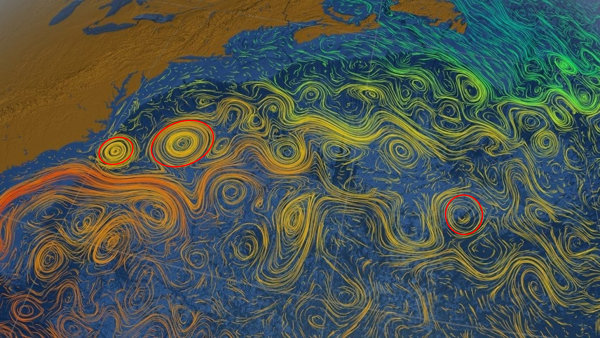
\includegraphics[width=14cm]{chapter/figure/visible eddies and currents in the North Atlantic.png}
  \caption
  {Image of visible eddies and currents photographed by NASA} 
  \label{visible eddies and flow}
\end{figure}


Figure \ref{visible eddies and flow} is a snapshot of Perpetual Ocean which shows ocean surface currents produced by model output (ECCO2). We could observe a lot of spiral-shaped eddies (markded in red circles) which trap certain amount of water inside in the figure.

	
Figure \ref{Plankton Bloom} shows how eddies deflect the density interfaces, deepen or shallow pycnocline (two density surfaces are seasonal thermocline $\rho_1$ and main thermocline $\rho_2$), and generate associated upwelling or downwelling. Thus nutrients can be brought up to the surface and down to the interior during the evolution of the eddies, which means that eddies directly affect the biogeochemistry process.

\begin{figure}[ht]
  \centering
  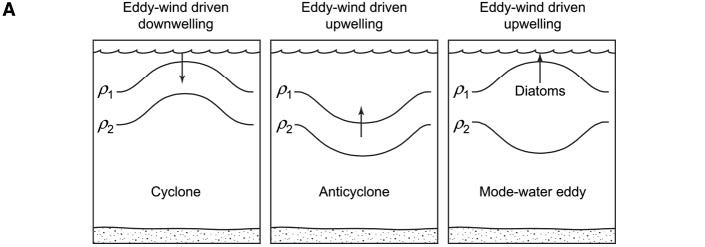
\includegraphics[width=15cm]{chapter/figure/Plankton Blooms.jpg}
  \caption
  {Isopycnal displacements associated with three types of eddies \cite{mcgillicuddy2007eddy}} 
  \label{Plankton Bloom}
\end{figure}

Previous studies have shown that eddy-induced fluid volume zonal transport can reach up to $ 30\sim40 $ Sv, which is as much as the large-scale wind-driven or  thermohaline circulation \cite{zhang2014oceanic}. In figure \ref{zonal transport of fluid carried by mesoscale eddies}, part A of the figure shows us the result of eddy-induced zonal transport per latitude based on the mean eddy propagation speed and trapped fluid volume while part B of the figure illustrates the total meridionally integrated zonal transport induced by eddies (blue curve here represents the westward transport and the red curve represents the eastward transport).The studies serve as the evidence of mesoscale eddies' role in the heat, energy, and flux transport.

\begin{figure}[ht]
  \centering
  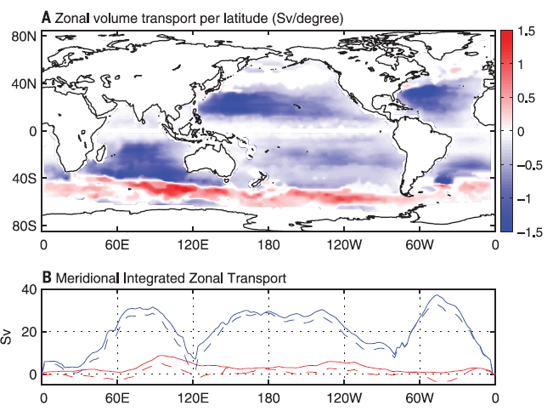
\includegraphics[width=15cm]{chapter/figure/Global distribution of the zonal and meridional transport of fluid trapped by mesoscale eddies.png}
  \caption
  {Global distribution of the zonal water transport carried by eddies 
  \cite{zhang2014oceanic} }
  \label{zonal transport of fluid carried by mesoscale eddies}
\end{figure}

The tremendous advances in ocean observational methods, especially measurements of ocean surface sea level anomaly, and altimetry-derived velocity fields enable the long-term detection of mesoscale vortices. An increasingly high-resolution and submesoscale-permitting ocean circulation model provides a panoramic view of the three-dimensional ocean flow.

Thus, detection and tracking of coherent ocean eddies have increasingly become a research hot spot.  

\section{The flow pattern of the Argentine Basin}\label{flow pattern of the Argentine Basin}

The Argentine Basin region, characterized by its basin structure, exhibits several different types of surface and subsurface currents and unique temperature and salt structures.

The Brazil‐Malvinas region is characterized by the confluence of southward transport Brazil Current (BC) and northward transport Malvinas Current (MC). Previous studies shows that BC transports about 25 Sv ( $ 1 \mathrm{Sv} = 10^6 m^3 s^{-1}$) warm ($\theta > 10^{\circ} \mathrm{C}$) and salt ($S > 35$) water and MC transports about 30-40 Sv cold ($\theta < 7^{\circ} \mathrm{C}$) and fresh ($S < 34.3$) water into the  Brazil‐Malvinas region \cite{jullion2010circulation}. The mixture of these two distinct water bodies would 
generate strong salinity and thermal gradient and cause mesoscale instabilities, which is expected to result in large amounts of oceanic eddies \cite{de2006multi}.

The great variability of the dynamic topography also gives rise to the anisotropic feature in the study region. For example, in the center of the Argentine Basin, Zapiola Anticyclone (ZA) is trapped by a seamount called the Zapiola Rise and the flow greatly inhibits the lateral transport of water, traps water inside, and increases vertical movement such as downwelling transport into the bottom Ekman layer \cite{weijer2020zapiola,frajka2019atlantic,dewar1998topography}.

What is more, the Argentine Basin is regarded as the main channel connecting the Southern Ocean and the Atlantic Ocean, and the properties of water masses inside the Argentine Basin are quite complicated. For example, looking down from the surface, the salinity of the surface-layer water is quite low, and the salinity becomes higher when it mixes with the North Atlantic Deep Water at about 1500-3500 m depth and it becomes a little fresher when it goes down into Antarctic Bottom Water \cite{talley2011descriptive}. The vertical distribution of water bodies is listed in the table \ref{Water mass vertical distribution} \cite{fontela2021anthropogenic}:

\doublerulesep 0.1pt
\begin{table}[htb]
  \centering
 \linespread{1.7}{ {\footnotesize
  \caption{Water mass vertical distribution}\label{Water mass vertical distribution}
\vspace{2em}
  \begin{tabular}{ccc}
  \hline
\noalign{\smallskip}
  \textbf{Water mass} & \textbf{Depth} & \textbf{Density $ \left(\mathrm{kg} \cdot \mathrm{m}^{-3}\right) $} \\
\noalign{\smallskip}
  \hline
  South Atlantic Central Water & 100 - 300 m & $\sigma \le 26.5 $ \\
  Sub Antarctic Mode Water & 300 - 600 m & $ 26.5<\sigma <27.1 $  \\
  Antarctic Intermediate Water & 600 - 1000m & $ 27.1<\sigma <27.4$ \\
  North Atlantic Deep Water & 1000 - 400 m & $ 27.4<\sigma < 45.90$ \\
  Antarctic Bottom Water & towards the sea floor & $ \sigma \ge 45.90$ \\
  \hline
\noalign{\smallskip}
  \end{tabular}
  }}
\end{table}

Due to the dynamic changes of the current and strong mixing in the study region, lots of energetic mesoscale eddies having great impact on heat and salt budgets were observed.


\section{Traditional vortex detection methods}\label{Eulerian representation}\label{Eulerian methods}

Traditional automated Eulerian eddy detection methods can be divided into three types \cite{nencioli2010vector}: physical parameter-based algorithm using the value exceeding a threshold to identify eddies, flow geometry-based methods focusing on the morphology of the instantaneous streamlines to extract vortices, and hybrid approach taking both the physical parameters and geometric features into consideration. 

McWilliams developed the earliest automatic eddy detection algorithm for decaying two-dimensional turbulence. The detection procedure is as follows: at first, we pick a two-dimensional extreme (maximum or minimum) in vorticity ($\xi$) as their center, and then identify the boundary as the points set with the criterion of $\frac{\xi}{\xi_c} \geqslant \Delta$ (${\xi_c}$ is the vorticity of the vortex center and $\Delta$ is the limiting value and 0.2 might be a satisfactory value) as shown in figure \ref{Closed vorticity contour in the turbulence flow}. Besides setting vorticity as the physical parameter, geometric characteristics are also taken into consideration: several shape quantities are raised to ensure that the boundary and interior of the candidate eddy should not depart excessively from asymmetry \cite{mcwilliams1990vortices}. This method belongs to the hybrid one.

\begin{figure}[ht]
  \centering
  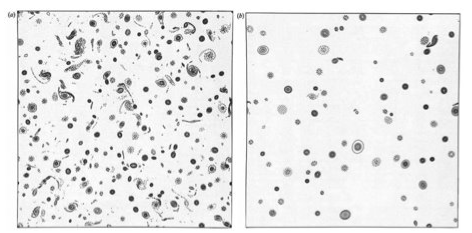
\includegraphics[width=15cm]{chapter/figure/closed vorticity contour in the turbulence flow.png}
  \caption
  {Closed vorticity contour in the turbulence flow 
  \cite{mcwilliams1990vortices} }
  \label{Closed vorticity contour in the turbulence flow}
\end{figure}

Among the overall methods, the most popular Eulerian methods are the SSHA method(\cite{roemmich2001eddy}), and Okubo-Weiss method. SSHA method considers sea level anomalies exceeding a threshold as an eddy and consider the local minimum (maximum) of SSH for cyclonic (anticyclonic) eddies \cite{chelton2011global}. However, this method lacks the ability to distinguish wave-like structures with eddies. Okubo-Weiss method detects eddies based on Okubo-Weiss parameter, W, which defines eddies by stretch ($s_{s}$), shear ($s_{n}$), and relative vorticity ($\omega$) in the flow field and the rotation-dominated case ($W < 0$) is considered as vortex \cite{calil2008eddy,chelton2007global}. $W=-2 \times 10^{-12} \mathrm{~s}^{-2}$ contours is used to extract eddies in global study.

\begin{equation}
    W=s_{s}^{2}+s_{n}^{2}-\omega^{2} 
\end{equation}

\begin{equation}
    s_{n}=\frac{\partial u^{\prime}}{\partial x}-\frac{\partial v^{\prime}}{\partial y}, \quad s_{s}=\frac{\partial v^{\prime}}{\partial x}+\frac{\partial u^{\prime}}{\partial y}, \quad w=\frac{\partial v^{\prime}}{\partial x}-\frac{\partial u^{\prime}}{\partial y}
\end{equation}

Via geostrophic balance, $u^{\prime}$ and $v^{\prime}$ may be calculated by the gradient of sea level anomaly.

\begin{equation}
    u^{\prime}=-\frac{g}{f} \frac{\partial(SLA)}{\partial y}, \quad v^{\prime}=\frac{g}{f} \frac{\partial(SLA)}{\partial x}
    \label{Geostrophic anomaly velocity}
\end{equation}

\begin{figure}[ht]
	\centering
	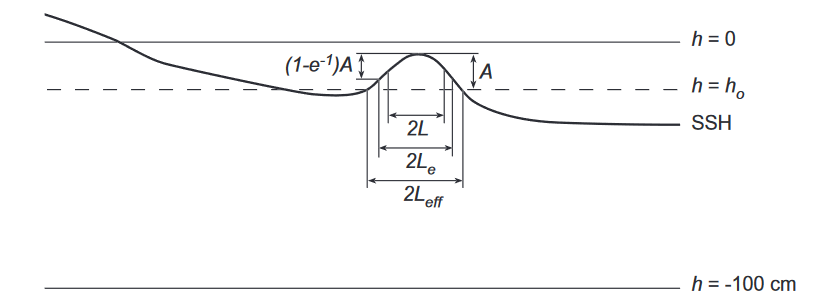
\includegraphics[width=15cm]{chapter/figure/A schematic summary of the automated eddy identification procedure for the case of an anticyclonic eddy.png}
	\caption
	{A schematic summary of the automated eddy identification procedure for the case of an anticyclonic eddy 
		\cite{chelton2011global} }
	\label{A schematic SSHA anticyclonic eddy}
\end{figure}

However, above Eulerian diagnostics are unreliable since they are not objective and depend on thresholds. Being not objective means that the results would perform differently when viewed from different reference frames. In other words, the existence of the eddy is questionable and the transport of material carried by eddy is not guaranteed to be coherent. Depending on thresholds signifies that the results of the detection would vary a lot and the boundary would disagree with each other when choosing different thresholds. In the following chapter \ref{Coherent vortices and geodesic theory}, we would turn to a new concept of Lagrangian coherent structures and how it is related to the detection of oceanic eddies.

\clearpage 

\section{Lagrangian coherent structures}\label{Coherent vortices and geodesic theory}

Recently, breakthroughs at the crossroads of nonlinear dynamical systems theory and fluid dynamics has promoted the application of detecting the vortices in a variety of fields. As shown in figure \ref{Lagrangian coherent structures}, in the field of dynamical systems, Lagrangian coherent structures (LCSs) refer to material lines or surfaces that attract, repel, or shear the most, which uncover the geometric property of the flow field (repelling LCSs tends to induce local stretching, thinning, and folding happen along attracting LCSs boundary, and shear LCSs describe swirling pattern \cite{haller2000lagrangian}), and thus play a significant role in the study of chaotic advection and material mixing \cite{haller2015lagrangian,aref2017frontiers,bettencourt2012oceanic}. Material coherence is observable everywhere in nature: Great Red Spot  photographed by Voyager 1 in 1979 and processed by Bjorn Jonsson as shown in figure \ref{red spot}. Because LCSs could influence the particles around them more than others, which means that this structure is not transient, thus a structure is considered coherent if it lasts a long time in the flow of the observed fluid \cite{peacock2013lagrangian}. In other words, LCSs could not be crossed by material and act as transport barrier, thus providing solid framework to detect coherent eddies.      

\begin{figure}[ht]
  \centering
  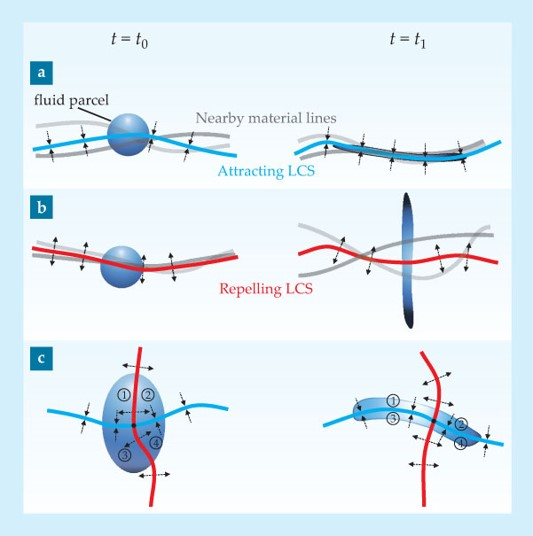
\includegraphics[width=7cm]{chapter/figure/Lagrangian coherent structures.jpg}
  \caption
  {Lagrangian coherent structures
  \cite{peacock2013lagrangian}} 
  \label{Lagrangian coherent structures}
\end{figure}

\begin{figure}[ht]
  \centering
  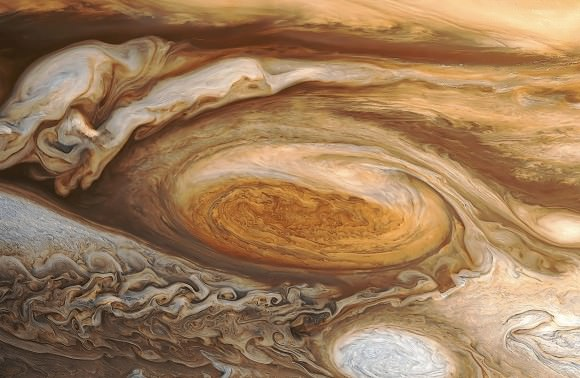
\includegraphics[width=13cm]{chapter/figure/coherent structure and red spot.jpg}
  \caption
  {Observable Coherent Lagrangian patterns(The Great Red Spot)
  \cite{haller2015lagrangian}} 
  \label{red spot}
\end{figure}

Instead of observing fluid properties from a fixed frame in chapter \ref{Eulerian representation} (Eulerian representation), Lagrangian dynamics focus on the motion of specific parcels of fluid and follow them through space \cite{price2006lagrangian}. Assessment of flow patterns from a single tracer is impractical because of the sensitivity of fluid-particle trajectories to initial conditions; however, LCSs provide a solid framework of material surfaces and thus enable the comparison of models and other observational data\cite{haller2015lagrangian}. 

However, LCSs in ocean turbulence are not well-defined and interpreted as material loops showing little deformation, no filamentation, and consistent area during the so-called LCSs life cycle, which would last for several weeks to several months. LCSs are believed to be bounded by uniformly stretching fluid line and maintain the arc length during the transport period. Such coherent structures will confine mixing and material exchange between the water body trapped inside and ambient ocean turbulent flow and thus quantify important aspects of material transport\cite{haller2015lagrangian}.

Recently, several Lagrangian methods have been developed to accurately predict the material transport barrier in geophysical flows: ridges of finite-time
Lyapunov exponent (FTLE) \cite{shadden2005definition, haller2011lagrangian}, and finite-size Lyapunov exponent (FSLE) \cite{aurell1997predictability, joseph2002relation, d2004mixing}. Haller proposed that the ridge of FTLE would be an indicator of hyperbolic LCSs (repelling in forward time and attracting in backward time) \cite{haller2001distinguished}. However, it still remains uncertain about the relationship between FTLE or FSLE with LCS and some counterexamples have doubted the robustness of the detection method \cite{haller2011variational, karrasch2013finite}. As shown in figure \ref{LCS and FTLE}, there is an observable repelling LCS along y-axis in the nonlinear strain flow while FTLE ridges are not detected in this case (constant forward FTLE field) \cite{haller2011variational}. In classic dynamical systems, this recurrent structure is called the saddle fixed point.

\begin{figure}[ht]
  \centering
  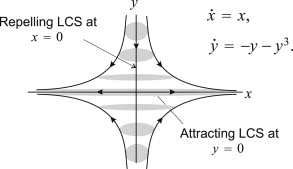
\includegraphics[width=12cm]{chapter/figure/mismatch.jpg}
  \caption
  {A mismatch between a repelling LCS and FTLE ridges\cite{haller2011variational}
  \label{LCS and FTLE}
  }
\end{figure}

In order to reduce the false positive and false negative results in coherent structure detection, a redefinition with rigorous mathematics is needed. 

\clearpage

\section{Dynamic Mechanisms of the  Mesoscale Eddy}

According to previous studies, the properties and formation of eddies were strongly related to the evolution of baroclinic instability caused by vertical velocity shear between different layers \cite{feng2021four,verma2021lagrangian}.

%and the existing distinct seasonal variation in eddy kinetic energy (EKE) may be related to the seasonal circle of vertical velocity shear change.

Complex flow-vortex interactions with strong currents near the western boundary could also explain the complicated LCSs in the study region.
 
Other dynamical factors such as mixed layer instabilities, frontal dynamics, buoyancy anomalies produced by sea ice leads and so on could also affect the formation and evolution process of LCSs \cite{mukiibi2016three,cohanim2021dynamics}.

How relative wind stress acts on eddies is controversial: some researchers think that it would depress the development of eddies and performs as the ``killer" of eddies' kinetic energy \cite{xu2016work,renault2019remarkable}; however, an updated study have demonstrated that eddies can response and adjust to the wind and the work done by relative wind stress on eddies could turn from negative to positive after the "inflection point" \cite{teng2021does}.

\clearpage

\section{Main content and Organization of the paper}

As mentioned above, studies of mesoscale eddies are now the research hotspots due to the importance of eddies' role. However, studies of basic statistical characteristics of the vortex, the three-dimensional structure of the vortex, and its influence on the vertical distribution of temperature and salt are not very clear in Argentine Basin. We want to understand the following questions: (1) How deep do the ocean eddies extend? (2) What is the shape of ocean eddies? (3) How many eddies could be detected and what are the characteristic features of the ocean eddies? (4) Given the same domain and same velocity field generated by the numerical model, how different it will be when different methods are adopted?

The thesis includes six chapters, and it starts with a brief introduction to the ocean eddies detection methods and flows pattern of the Argentine Basin. Chapter Two mainly discuss the detailed setup process of the eddy’s detection.

Chapters Three to Five contain the main body of this thesis and cover the eddies properties, three-dimensional eddies profile, and comparison of several different methods in the eddy detection process. The last chapter draws a general conclusion from the above content and outlines several future research directions.

To be specific, Chapter Two gives mathematical images and formulas of nonlinear dynamics and geodesic theory and its application to geostrophic flow. Since the content is not intuitive enough, someone who is not familiar with the notion may skip this chapter and backtrack the chapter as a reference when needed. What is more, we also discuss the drawback of traditional Eulerian method, which is the base of Chapter Three.

Chapter Three focuses on the comparison of Eulerian methods and Lagrangian methods and verifies the robustness of LAVD method. The similarities and differences between these results are discussed here.

Chapter Four concerns the statistical quantity of the ocean eddies such as their radius, polarity and population. We show that most eddies maintain their coherent feature during the transport, which lays a solid foundation for accurately quantifying the eddies-induced transport in Argentine Basin.

In Chapter Five, we explore the three-dimensional structure of the vortex and discuss the vertical extension of eddies from the surface to subsurface. 

Chapter Six makes a conclusion of the work and provides an outlook and forecast of possible future work.

\newpage

\chapter{data and methodology}\label{data and methodology}

In this chapter, we first introduce the data used in the study, and the flow pattern of the research area. Then, we give a brief introduction to the available velocity-based estimates of oceanic eddies, summarize their characteristics and point out their limits and deficiency such as the inability of capturing long-term transport mechanisms and inconsistency in different reference frames. At last, we focus on the computation setup workflow of the objective Lagrangian eddy detection methods.


\section{Research background}

\subsection{Data description}

In the study, we combine the remote sensing satellite altimetry data and oceanic model data.

Satellite altimetry gives a new perspective on sea surface topography anomaly observation by providing full coverage of the ocean surface measurements. By analyzing sea level anomaly (SLA) from the \href{https://www.aviso.altimetry.fr/en/home.html}{AVISO product} (https://www.aviso.altimetry.fr/en/home.html) between January 1993 to December 2019, we can learn the long-term climatology characteristics of the oceanic eddies. AVISO SLA data combines a series of satellites data such as Ocean Topography Experiment
(TOPEX) / Poseidon and European Remote Sensing Satellite (ERS) altimeter data, and then all the weekly product was interpolated to $\frac{1}{4}^{\circ} \times \frac{1}{4}^{\circ}$ spatial resolution grid points based on the Mercator projection method, which provides oceanographer with solid and continuous upper ocean mesoscale information \cite{beron2018enduring,ducet2000global,xu2019oceanic,laxenaire2018anticyclonic}.

Ocean model data provides us with three-dimensional oceanic flow information, which contributes to the three-dimensional construction of ocean vortex structures and helps us understand the volume transport. In the study, we apply the same methodology to the Southern Ocean State Estimate (SOSE) dataset at each depth level and the time span is from 2013 to 2018, which covers part of the time period of the AVISO altimetry data \cite{mazloff2010eddy,verdy2017data}. Thus, we could construct the three dimensional structures and calculate  mass transport carried by eddies \cite{dong2012three}.

%The study region was set to be bounded by latitude from 60 S to 30 S and longitude from 70 W to 30 W, which covered the whole Argentine Basin, South American Coast, and part of the connecting Southern Ocean. The southern edge of the domain is located in the northern part of the Southern Ocean in order to study the water and mass exchange; the northern margin of the region is affected by the confluence of Brazil Current water masses.


The flow velocity is established on the basis of geostrophic balance theory which assumes that the sea pressure gradient force induced by sea surface slope and Coriolis force are approximately equal:

\begin{equation}
\mathbf{v}(\mathbf{x}, t)=\left[-\frac{g}{f} \frac{\partial \eta(\mathbf{x}, t)}{\partial y}, \frac{g}{f} \frac{\partial \eta(\mathbf{x}, t)}{\partial x}\right] 
\end{equation}


$\mathbf{x}=(x, y)$ denotes the zonal and meridional velocity; $\eta(\mathbf{x}, t)$ denotes sea surface height (SSH); $f$ is the vertical component of Coriolis force; and $g$ is the acceleration of gravity \cite{beron2013objective}.

The variation of SSH is calculated from the gap between altimeter SSH anomaly data and the mean dynamic topography. The background $\eta$ is assumpted to be steady and the perturbation part of SSH is transient.

\subsection{Introduction to the study area}

The latitude range of the research area is between 30S and 60S and the longitude ranges from 70W to 30W as shown in figure \ref{research topography}. The main study region could be separated into four zones:  Argentine Basin (AB) covering most of the northeast part of the study region; Southern Ocean (SO) region; connecting waters between AB and SO. The Argentine Basin is of flattened-circular shape and bounded by Patagonian Shelf to the west and Rio Grande Rise to the north \cite{weijer2015eddy}. We could learn from the map that the central part of the basin is deeper than 4,000 meters and it can reach 600 meters at the southwestern part. South Georgia and the South Sandwich Islands and Falkland Islands lie in the east and west of the study area.

\begin{figure}[hbtp]
  \centering
  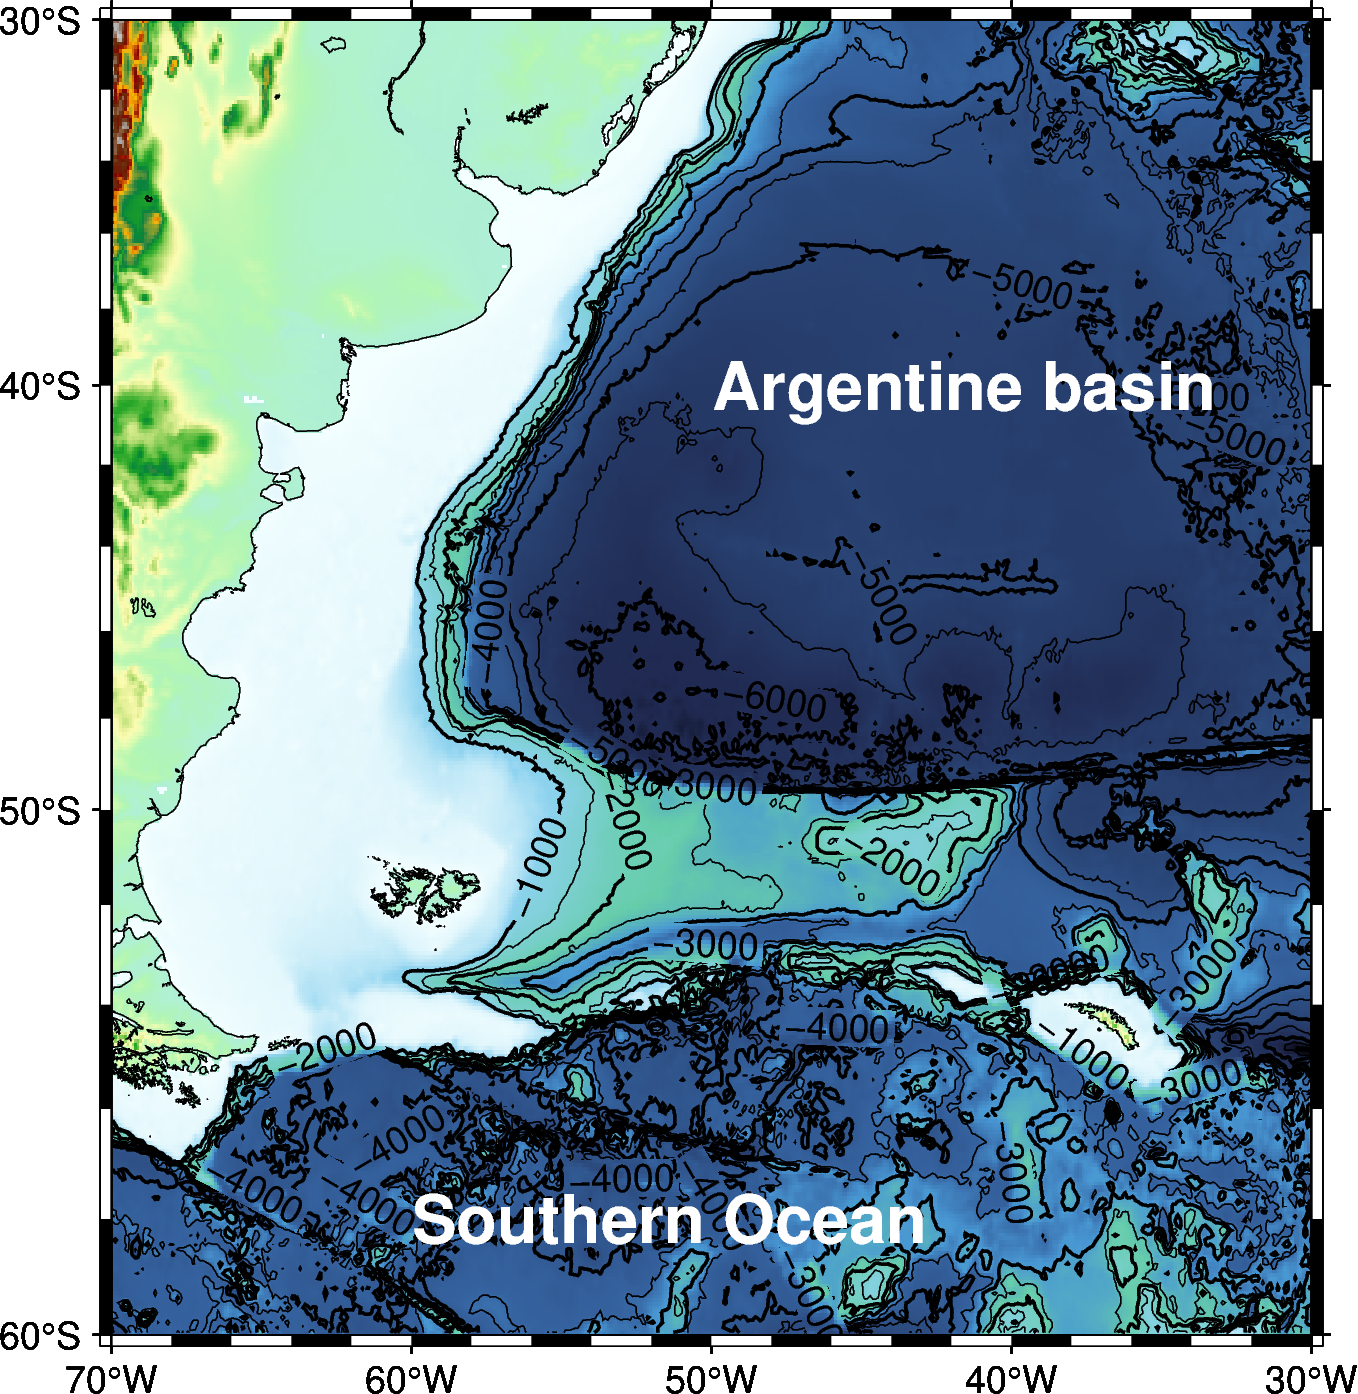
\includegraphics[width=15cm]{chapter/figure/research area topography map_earth.png}
  \caption
  {Topographic map of the research region}
  \label{research topography}
\end{figure}

The surface flow pattern of the research region is shown is figure \ref{surface flow pattern} and has already been descried in chapter \ref{flow pattern of the Argentine Basin} to show the importance of the study. Southward transport Brazil Current (BC) mix with northward transport Malvinas Current (MC) and form fluctuating Brazil/Malvinas Confluence (BMC) at about 40°S due to wind stress and baroclinic instabilities \cite{jullion2010circulation,weijer2015eddy}. An anticyclonic gyre called Zapiola Anticyclone (ZA) around the hill transports considerably large volume of water of about 200 Sv \cite{saunders1995bottom}. 

\begin{figure}[hbtp]
  \centering
  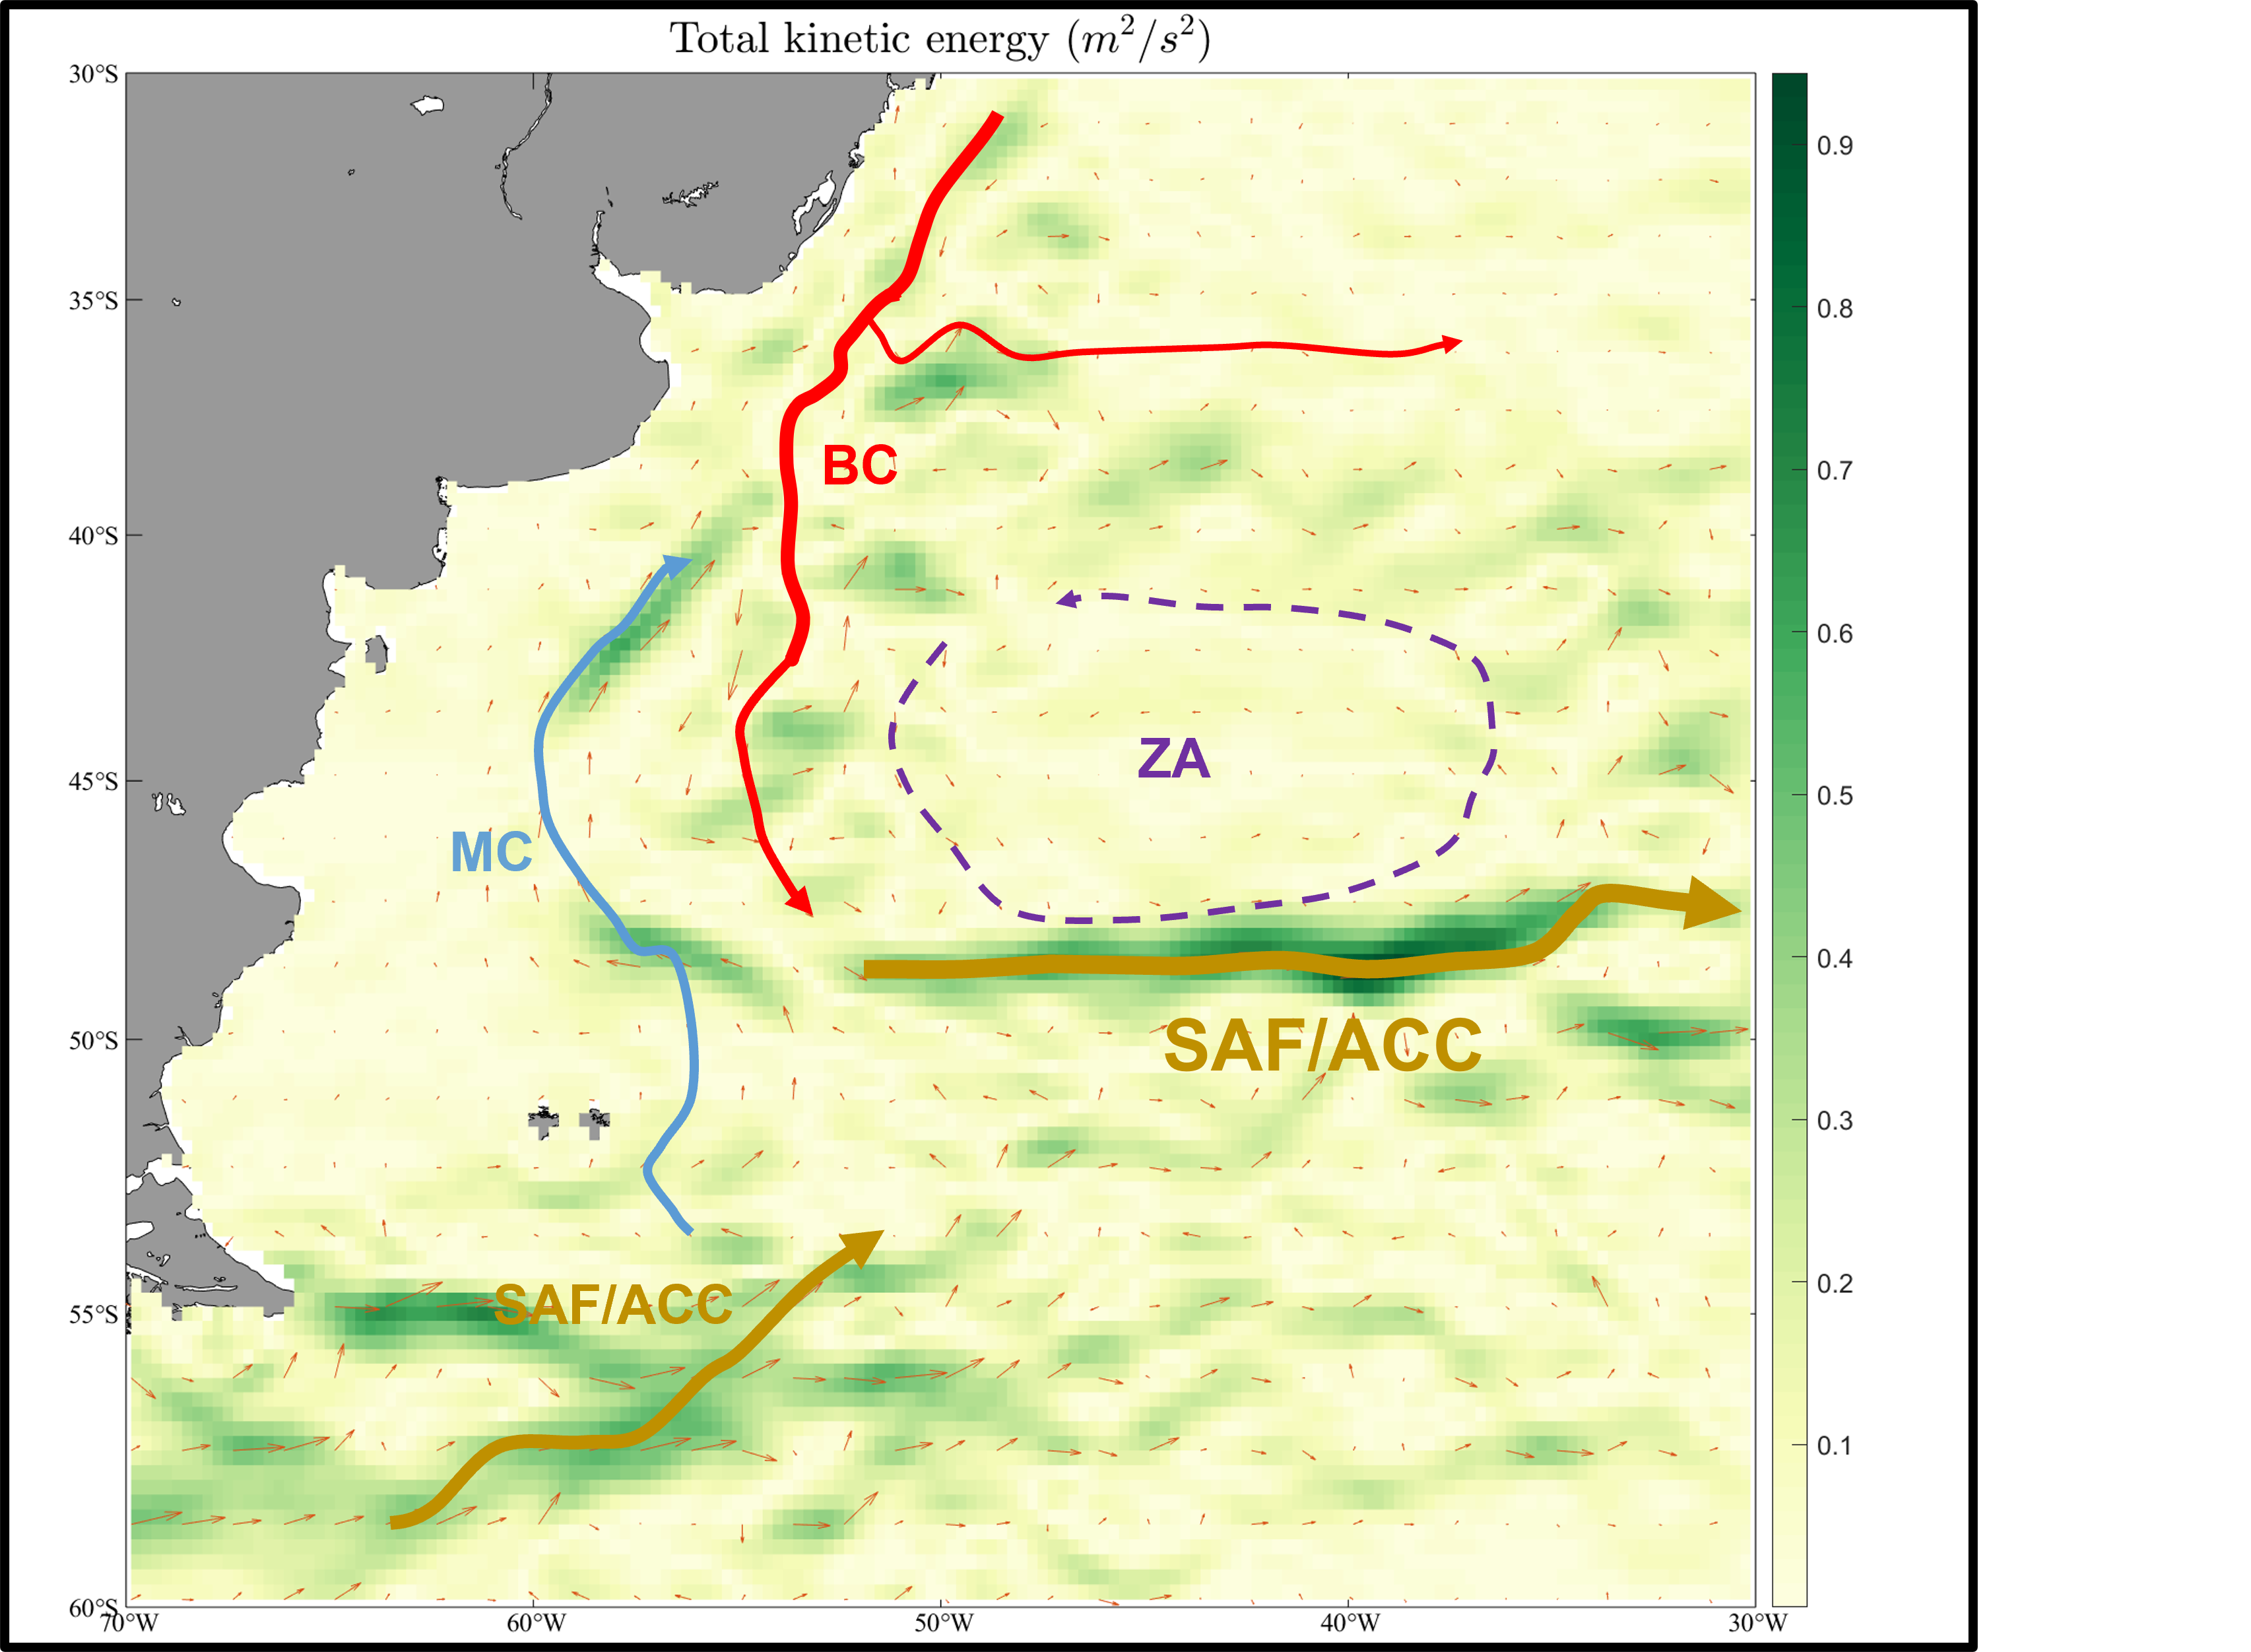
\includegraphics[width=15cm]{chapter/figure/surface flow with notion.png}
  \caption
  {Surface current pattern of the research area}
  \label{surface flow pattern}
\end{figure}

\section{Traditional Eulerian method and its drawback}

Since oceanic eddies are regarded as swirling bodies of water that trap a certain number of tracers inside, oceanic eddies are widely acknowledged to be Lagrangian (material).

There are two analytical frameworks for fluid mechanics study: one is the Eulerian method to describe the dynamics properties in a fixed space and the other is the Lagrangian method to describe the fluid properties from the point of view of particle motion \cite{kasten2011extraction}. 

Traditional eddy detection methods are Eulerian methods based on the instantaneous velocity field, which are not robust and may produce spurious results. For example, one of the Eulerian criteria is to seek a closed streamline in unsteady fluid flows; however, this topological feature is not invariant under Galilean transformations, and thus closed streamline may behave differently when choosing different Galilean transformation schemes \cite{kasten2011extraction}.

% Another way to extract vortex is based on scalar quantities such as $Q$ and $\lambda_2$, and these quantities are based on the Jacobian matrix of the flow field and thus are Galilean invariant.

As well as the above problems, Eulerian methods depend on the chosen thresholds value, thus the detection result could vary a lot when choosing different thresholds, generating noisy results and making the quantification of eddy transport unreasonable. 

\section{Objective Lagrangian eddies detection}\label{Lagrangian eddies detection}

In the last section, we discussed some Eulerian eddy-detection methods which are suitable for analysis of snapshot properties but not for distinguishing long-living structures from the incoherent unsteady flow.

Thus, more attention has been paid to the Lagrangian point of view and characterizes flow patterns in the path line.

The theory for extracting the material boundaries in steady or near-steady flow has been put forward for more than two decades; however, identifying material boundaries in unsteady flow has been a question for long time. Recently, Haller and Beron-Vera developed a new approach to describe transport barrier as the least stretching material line and the closed shearline of $\gamma_{t_0}$. The elliptic transport barrier is computed in the period of $[t_0,t+T]$, acting as the generalized KAM curve and conserving both its arclength and enclosed area until $t_0+T$ \cite{haller2012geodesic}. Thus, the elliptic transport barrier is the desired organization of the eddy candidate region.

The above theory seeks those frame-independent maximal shear as transport barriers and the shear barriers with a bunch of closed curves are called elliptic barriers \cite{wang2015identification}. The outermost elliptic barrier serves as the eddy boundary and enclosed the maximum area of coherent water mass over the domain\cite{wang2015identification}. 

\subsection{Computation setup}

We begin a two-dimensional velocity field $ \mathbf{v}(\mathbf{x},t)$, with $\mathbf{x}$ representing the position in the flow field and fix the time span ($[t_0,t_0+T]$) for tracking the coherent eddies.


\begin{equation}
    \dot{\mathbf{x}}(t)=\mathbf{u}(\mathbf{x}(t), t)
\end{equation}


For two-dimensional, divergence-free flows, we could introduce the stream function $\mathbf{\Psi}(x,y)$and rewrite the velocity in the form of gradient of the stream function. This conversion links the Hamiltonian mechanics and 2-D unsteady flow and makes the detection of invariant manifolds under the flow possible \cite{aref2017frontiers}.

\begin{equation}
    u=\frac{d x}{d t}=\frac{\partial \mathbf{\Psi}}{\partial y}, \quad v=\frac{d y}{d t}=-\frac{\partial \mathbf{\Psi}}{\partial x}
\end{equation}

We then introduce the concept of flow map $ F_{t_{0}}^{t_0+T} $. This map describes the Lagrangian trajectory of the particle released at initial position $x_0$ and how it evolves with time.

\begin{equation}
F_{t_{0}}^{t_0+T}: \mathbf{x}_{0} \mapsto \mathbf{x}\left(t_0+T;\mathbf{x}_{0}, t_{0}\right)
\end{equation}

In continuum fluid mechanics, we can describe the strain by introducing deformation gradient, and the following equation \ref{2-d DF} shows how to calculate deformation gradient in 2-dimensional flow fields.

%\begin{footnotesize} 
%\begin{align}
%    \nabla F_{t_{0}}^{t}\left(x_{0}\right) \approx\left(\begin{array}{cccc}
%\frac{x^{1}\left(t ; t_{0}, x_{0}+\delta_{1}\right)-x^{1}\left(t ; t_{0}, x_{0}-\delta_{1}\right)}{\left|2 \delta_{1}\right|} & \frac{x^{1}\left(t ; t_{0}, x_{0}+\delta_{2}\right)-x^{1}\left(t ; t_{0}, x_{0}-\delta_{2}\right)}{\left|2 \delta_{2}\right|} & \frac{x^{1}\left(t ; t_{0}, x_{0}+\delta_{3}\right)-x^{1}\left(t ; t_{0}, x_{0}-\delta_{3}\right)}{\left|2 \delta_{3}\right|} \\
%\frac{x^{2}\left(t ; t_{0}, x_{0}+\delta_{1}\right)-x^{2}\left(t ; t_{0}, x_{0}-\delta_{1}\right)}{\left|2 \delta_{1}\right|} & \frac{x^{2}\left(t ; t_{0}, x_{0}+\delta_{2}\right)-x^{2}\left(t ; t_{0}, x_{0}-\delta_{2}\right)}{\left|2 \delta_{2}\right|} & \frac{x^{2}\left(t ; t_{0}, x_{0}+\delta_{3}\right)-x^{2}\left(t ; t_{0}, x_{0}-\delta_{3}\right)}{\left|2 \delta_{3}\right|} \\
%\frac{x^{3}\left(t ; t_{0}, x_{0}+\delta_{1}\right)-x^{3}\left(t ; t_{0}, x_{0}-\delta_{1}\right)}{\left|2 \delta_{1}\right|} & \frac{x^{3}\left(t ; t_{0}, x_{0}+\delta_{2}\right)-x^{3}\left(t ; t_{0}, x_{0}-\delta_{2}\right)}{\left|2 \delta_{2}\right|} & \frac{x^{3}\left(t ; t_{0}, x_{0}+\delta_{3}\right)-x^{3}\left(t ; t_{0}, x_{0}-\delta_{3}\right)}{\left|2 \delta_{3}\right|}
%\end{array}\right)
%\label{3-d DF}
%\end{align}
%\end{footnotesize}

\begin{footnotesize} 
	\begin{align}
	\nabla F_{t_{0}}^{t}\left(x_{0}\right) \approx\left(\begin{array}{cccc}
	\frac{x^{1}\left(t ; t_{0}, x_{0}+\delta_{1}\right)-x^{1}\left(t ; t_{0}, x_{0}-\delta_{1}\right)}{\left|2 \delta_{1}\right|} & \frac{x^{1}\left(t ; t_{0}, x_{0}+\delta_{2}\right)-x^{1}\left(t ; t_{0}, x_{0}-\delta_{2}\right)}{\left|2 \delta_{2}\right|}  \\
	\frac{x^{2}\left(t ; t_{0}, x_{0}+\delta_{1}\right)-x^{2}\left(t ; t_{0}, x_{0}-\delta_{1}\right)}{\left|2 \delta_{1}\right|} & \frac{x^{2}\left(t ; t_{0}, x_{0}+\delta_{2}\right)-x^{2}\left(t ; t_{0}, x_{0}-\delta_{2}\right)}{\left|2 \delta_{2}\right|}  
	\end{array}\right)
	\label{2-d DF}
	\end{align}
\end{footnotesize}

In the above equation, $ \delta_{i} $ is a small vector pointing in the $ x^{i} $ coordinate direction.

The right Cauchy–Green strain tensor $\mathbf{C}_{t_{0}}^{t_{0}+T}\left(\mathbf{x}_{0}\right)$ is then
definded as 
\begin{equation}
    \mathbf{C}_{t_{0}}^{t_{0}+T}\left(\mathbf{x}_{0}\right)=\left(\nabla \mathbf{F}_{t_{0}}^{t_{0}+T}\left(\mathbf{x}_{0}\right)\right)^{\mathrm{T}} \nabla \mathbf{F}_{t_{0}}^{t_{0}+T}\left(\mathbf{x}_{0}\right)
\end{equation}


This symmetric tensor is positive definite, thus we could get two real positive eigenvalues $ \lambda_{i} $ and orthogonal real eigenvectors $ \xi_{i} $:

\begin{equation}
    C \xi_{i}=\lambda_{i} \xi_{i}, \quad\left|\xi_{i}\right|=1, \quad i=1, 2 ; \quad 0<\lambda_{1} \leq \lambda_{2}, \quad \xi_{i} \perp \xi_{j}, \quad i \neq j
\end{equation}

If the flow is incompressible, these two eigenvalues also satisfy the following relations:
 
\begin{equation}
     \operatorname{det} C=\prod_{i} \lambda_{i} \equiv 1,\quad0<\lambda_{1}<1<\lambda_{2}
\end{equation}



After setting up the invariant dynamical system, we now turn to scalar quantities.

The first technique is by using the Lyapunov exponent, which originates from dynamical system and measures how much close particles spread in the chaotic flow field. This method identifies LCSs as ridges in the Finite time Lyapunov exponent (FTLE) field and thus small or no material flux cross LCSs \cite{shadden2005definition, haller2001distinguished,haller2002lagrangian,haller2011lagrangian}. This method is widely used in ideal flow experiment.

The Finite time Lyapunov exponent $ \sigma $ is calculated as:

\begin{equation}
    \sigma\left(\mathbf{F}_{t_{0}}^{t_{0}+T}\left(\mathbf{x}_{0}\right) ; \mathbf{x}_{\mathbf{0}}\right)=\frac{1}{|T|} \log \sqrt{\lambda_{\max }\mathbf{C}\left(\mathbf{x}_{0}\right)}
\end{equation}

The second method is more rigorous mathematically and identifies the least stretching or deforming material surface (in 3-D flow) or material line (2-d flow) through a variational theory\cite{blazevski2014hyperbolic,haller2011variational,haller2012geodesic}. This method is more widely used in geophysical flows and recent studies of life cycle of a coherent Agulhas ring and detection of Agulhas Leakage have demonstrated its robustness\cite{wang2015identification,wang2016life,beron2013objective}. 
First, we assume an initial materine line to be $\mathcal{M}(t_0)$ and then it is advected to be $\mathcal{M}(t_0+T)$ according to equation \ref{material line}.

\begin{equation}
    \mathcal{M}(t_0+T):=F_{t_{0}}^{t_0+T}\left(\mathcal{M}\left(t_{0}\right)\right)
    \label{material line}
\end{equation}

To express this coherence principle mathematically, we select a parametrization $r(s)$ with $s \in[0, \sigma]$ for the closed curve $\gamma$ at time $t_{0}$, and denote the length of a tangent vector $r^{\prime}(s)$ by $l_{t_{0}}(s)$. We also let $l_{t_0+T}(s)$ denote the length of the corresponding tangent vector $(\mathrm{d} / \mathrm{d} s) F_{t_{0}}^{t_0+T}(r(s))$ along the advected curve $F_{t_{0}}^{t_0+ T}(\gamma) .$ These two tangent lengths can be calculated as

\begin{equation}
    l_{t_{0}}(s)=\sqrt{\left\langle r^{\prime}(s), r^{\prime}(s)\right\rangle}, \quad l_{t}(s)=\sqrt{\left\langle r^{\prime}(s), C_{t_{0}}^{t}(r(s)) r^{\prime}(s)\right\rangle}
\end{equation}

\begin{figure}[ht]
  \centering
  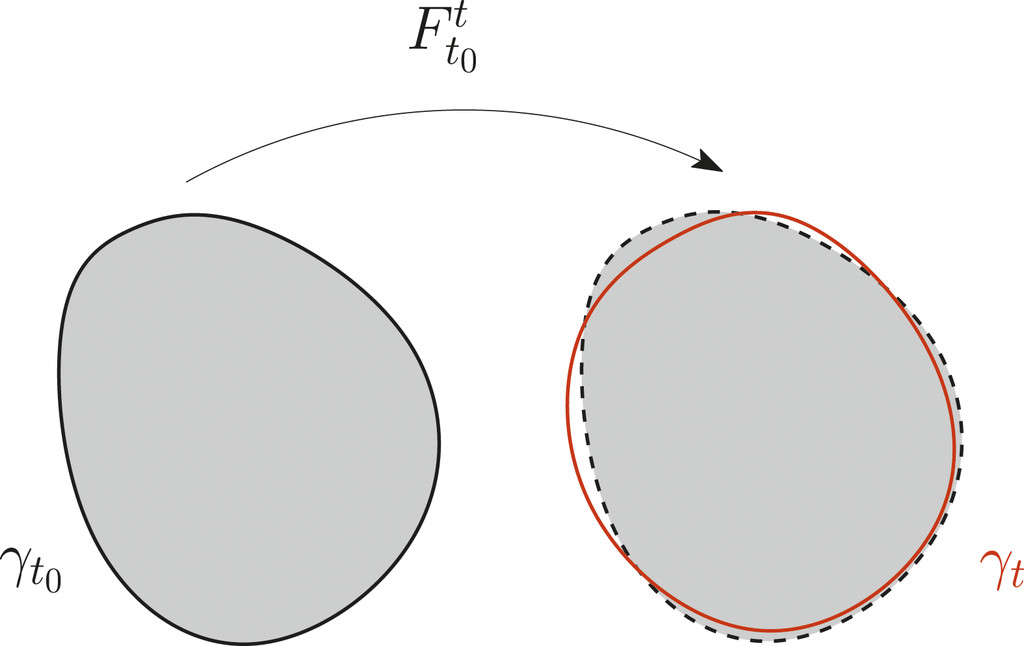
\includegraphics[width=15cm]{chapter/figure/Schematics of a closed shearline.jpg}
  \caption
  {Schematic of a closed shearline (elliptic transport barrier) \cite{beron2013objective}
  }
\end{figure}

where $\langle\cdot, \cdot\rangle$ denotes the Euclidean inner product \cite{truesdell2004non}. The averaged tangential strain along $\gamma$ is then given by

\begin{equation}
    Q(\gamma)=\frac{1}{\sigma} \int_{0}^{\sigma} \frac{l_{t_0+T}(s)}{l_{t_{0}}(s)} \mathrm{d} s
\end{equation}


As argued above, if an observable coherent material belt exists around $\gamma$, then on $\varepsilon$-close material loops we must have $Q(\gamma+\varepsilon h)=Q(\gamma)+O\left(\varepsilon^{2}\right)$, where $\varepsilon h(s)$ denotes small, periodic perturbations to $\gamma$. This is only possible if the first variation of $Q$ vanishes on $\gamma$ :

\begin{equation}
  \delta Q(\gamma)=0
\end{equation}


\begin{figure}[ht]
  \centering
  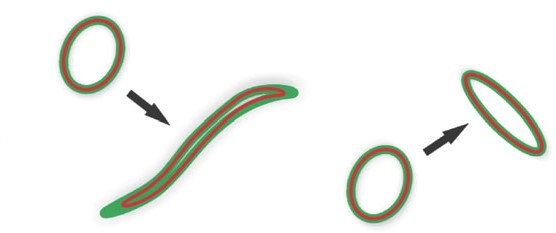
\includegraphics[width=15cm]{chapter/figure/Haller_Beron-Vera_2013_Coherent Lagrangian vortices_Journal of Fluid Mechanics.jpg}
  \caption
  {Comparison of ordinary material line and coherent material line \cite{haller2013coherent}
  }
  \label{material line compare}
\end{figure}

The third method for detecting the oceanic eddies is the Lagrangian Averaged Vorticity Deviation (LAVD) method, which is more intuitive and takes the time-integrated deviation of vorticity from background vorticity into consideration \cite{haller2016defining,tarshish2018identifying}. Using this method, vortex center is regarded as the maximum value of $|LAVD|$ and the vortex boundaries are the outermost convex curves around the center. We define coherence over a finite time interval $[t_0,t_0+T]$, which means that water column remain inside vortex during the period.


\begin{equation}
    LAVD_{t_0}^{t_0+T}(x_{0})=\int_{t_0}^{t_0+T}|\omega-\bar{\omega}| d s \quad 
\end{equation}

In the study, we apply LAVD eddy detection algorithm to altimetry-derived ocean currents starting on the first day of every month from 1993-2019, and the coherence time spans is 30 days. In the next step, we also change the time period from 30 days to 60 days, 90 days, and even 120 days and apply the methods to the model simulation product at each depth. Tracking coherent eddies in a 27-year period contributes to the understanding of the role of oceanic eddies in the transport process, especially the move of diffusive material and climatology trend of eddies change. The coherence time span varies to test the maximum material coherence of the eddies.

%We adopt fourth-order Runge–Kutta method in the interpolation process to get the eddy trajectories.

Thus, the workflow for us to apply the eddy detection algorithm to extract oceanic eddies from the flow field is as follows:

\begin{itemize}
  \item [1)] 
  Set up a two-dimensional velocity field to advect the particle.
  \item [2)]
  Introduce the definition of flow map to show how particles move in the coherent time interval $\Delta t$.
  \item [3)]
  Calculate the deformation gradient and get the Cauchy-Green Strain Tensor.
  \item[4)]
  Finally, we compute the LCSs from the LAVD field.
\end{itemize}

%Besides, we also use Eulerian methods in the study to validate the robustness of the result.

% \subsection{Calculation of eddies transport}

% \section{Some statistics about vortex}

% After setting up the dynamical system, and detecting the vortex center and boundary from the flow, we could compute some properties of the vortex.
% The area A of the vortex refers to the boundary contained within the boundary of the vortex, and the radius R is regarded as the radius of a circle of the equal area $R = \sqrt{A/\pi}$.

% Geostrophic velocity anomaly was shown in equation \ref{Geostrophic anomaly velocity}, which is derived from the gradient of the SLA. Eddy kinetic energy (EKE) is half of the sum of the squares of the geostrophic velocity anomaly:

% \begin{equation}
%     EKE=\frac{1}{2}\left(u^{\prime 2}+v^{\prime 2}\right)
% \end{equation}

% After calculating the EKE, we could then define a parameter called eddy intensity to describe the average eddy kinetic energy normalized by vortex area.

% \begin{equation}
%     EI=\frac{\langle EKE\rangle}{A}=\frac{\langle EKE\rangle}{\pi R^{2}}
% \end{equation}





\newpage

%\chapter{Eddies features analysis} \label{Eddies features analysis}

In this chapter, we present statistical results of coherent Lagrangian eddies using LAVD method.



\section{Eddies statistics}\label{Eddies statistics}

This chapter includes a set of figures showing census statistics about the eddies detected and tracked by applying LAVD method to AVISO dataset. Over the period of 1993-2019, 6212 coherent eddies with radius larger than 20 km and coherence time of 30 days were detected.

The figure \ref{fig:eddy number} shows the monthly and yearly variation patterns of the eddy number. From the figure, we could infer that the number of eddies distributes unevenly in four seasons and shows a trend of increasing from 1993 to 2019. The average number of eddies per month is about 20 and it ranges from 10 to 40. Eddies' number rises to 41, and peaks in December 2014. The months with the fewest eddies were Feb 2000, Apr 2007, Jun 1994, and Oct 2010, and only 10 eddies were detected in those months as shown in section (c) of the figure \ref{fig:eddy number}.  

In December, around 600 eddies were detected from 1993 to 2019 while only 452 eddies were detected in June. Seasonal change of eddy number shows that eddy number peaks in summer, decreases rapidly, and reaches the minimum value in winter. From (b) part of the figure \ref{fig:eddy number}, we could come to a conclusion that eddies number increases over the last three decades, showing a hint of how global warming would increase the instability of the upper ocean and the increasing rate is 3/year.

\begin{figure}
    \centering
    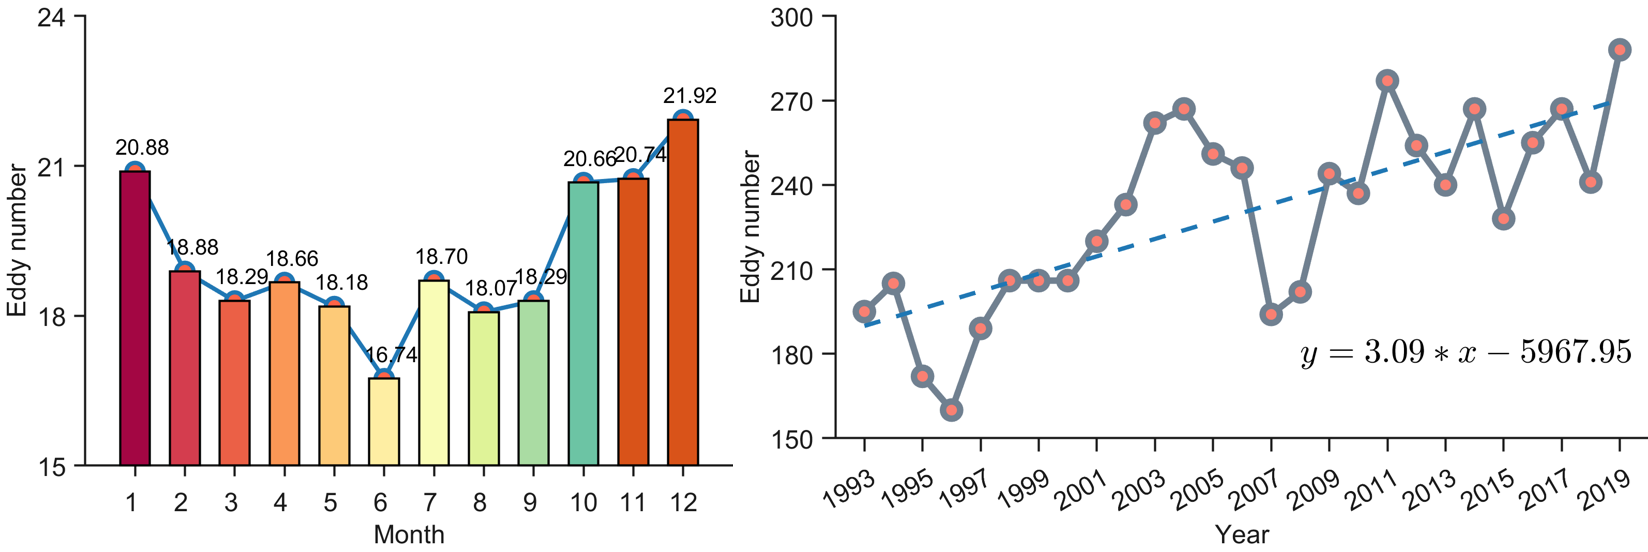
\includegraphics[width = 15cm]{chapter/figure/Eddy number per month and per month.png}
    \caption{Eddy number per month and per month}
    \label{fig:eddy number}
\end{figure}

The average eddy radius is 32.98 km and the standard deviation is 11.31 km. From the eddy radius histogram as shown in section (c) of the figure \ref{Eddy radius map}, we could infer that most of the eddies fall within the range of 20-30 km. The frequency of eddy radius decreases exponentially with increasing radius. From section (b) of the figure \ref{Eddy radius map}, eddy radius does not show an upward or downward trend year by year. Eddies that were generated in 2019 show an average maximum value of 34.41 km while eddies reached the minimum value (31.3 and 31.5 km) in 1996 and 1997. The monthly change of eddy radius shows a minimum value in July and August and a maximum value in December.

Combining the information on eddy number and eddy radius, we may come to the conclusion that in winter, the number and radius of eddies will be reduced due to insufficient energy in the upper ocean.

\begin{figure}
    \centering
    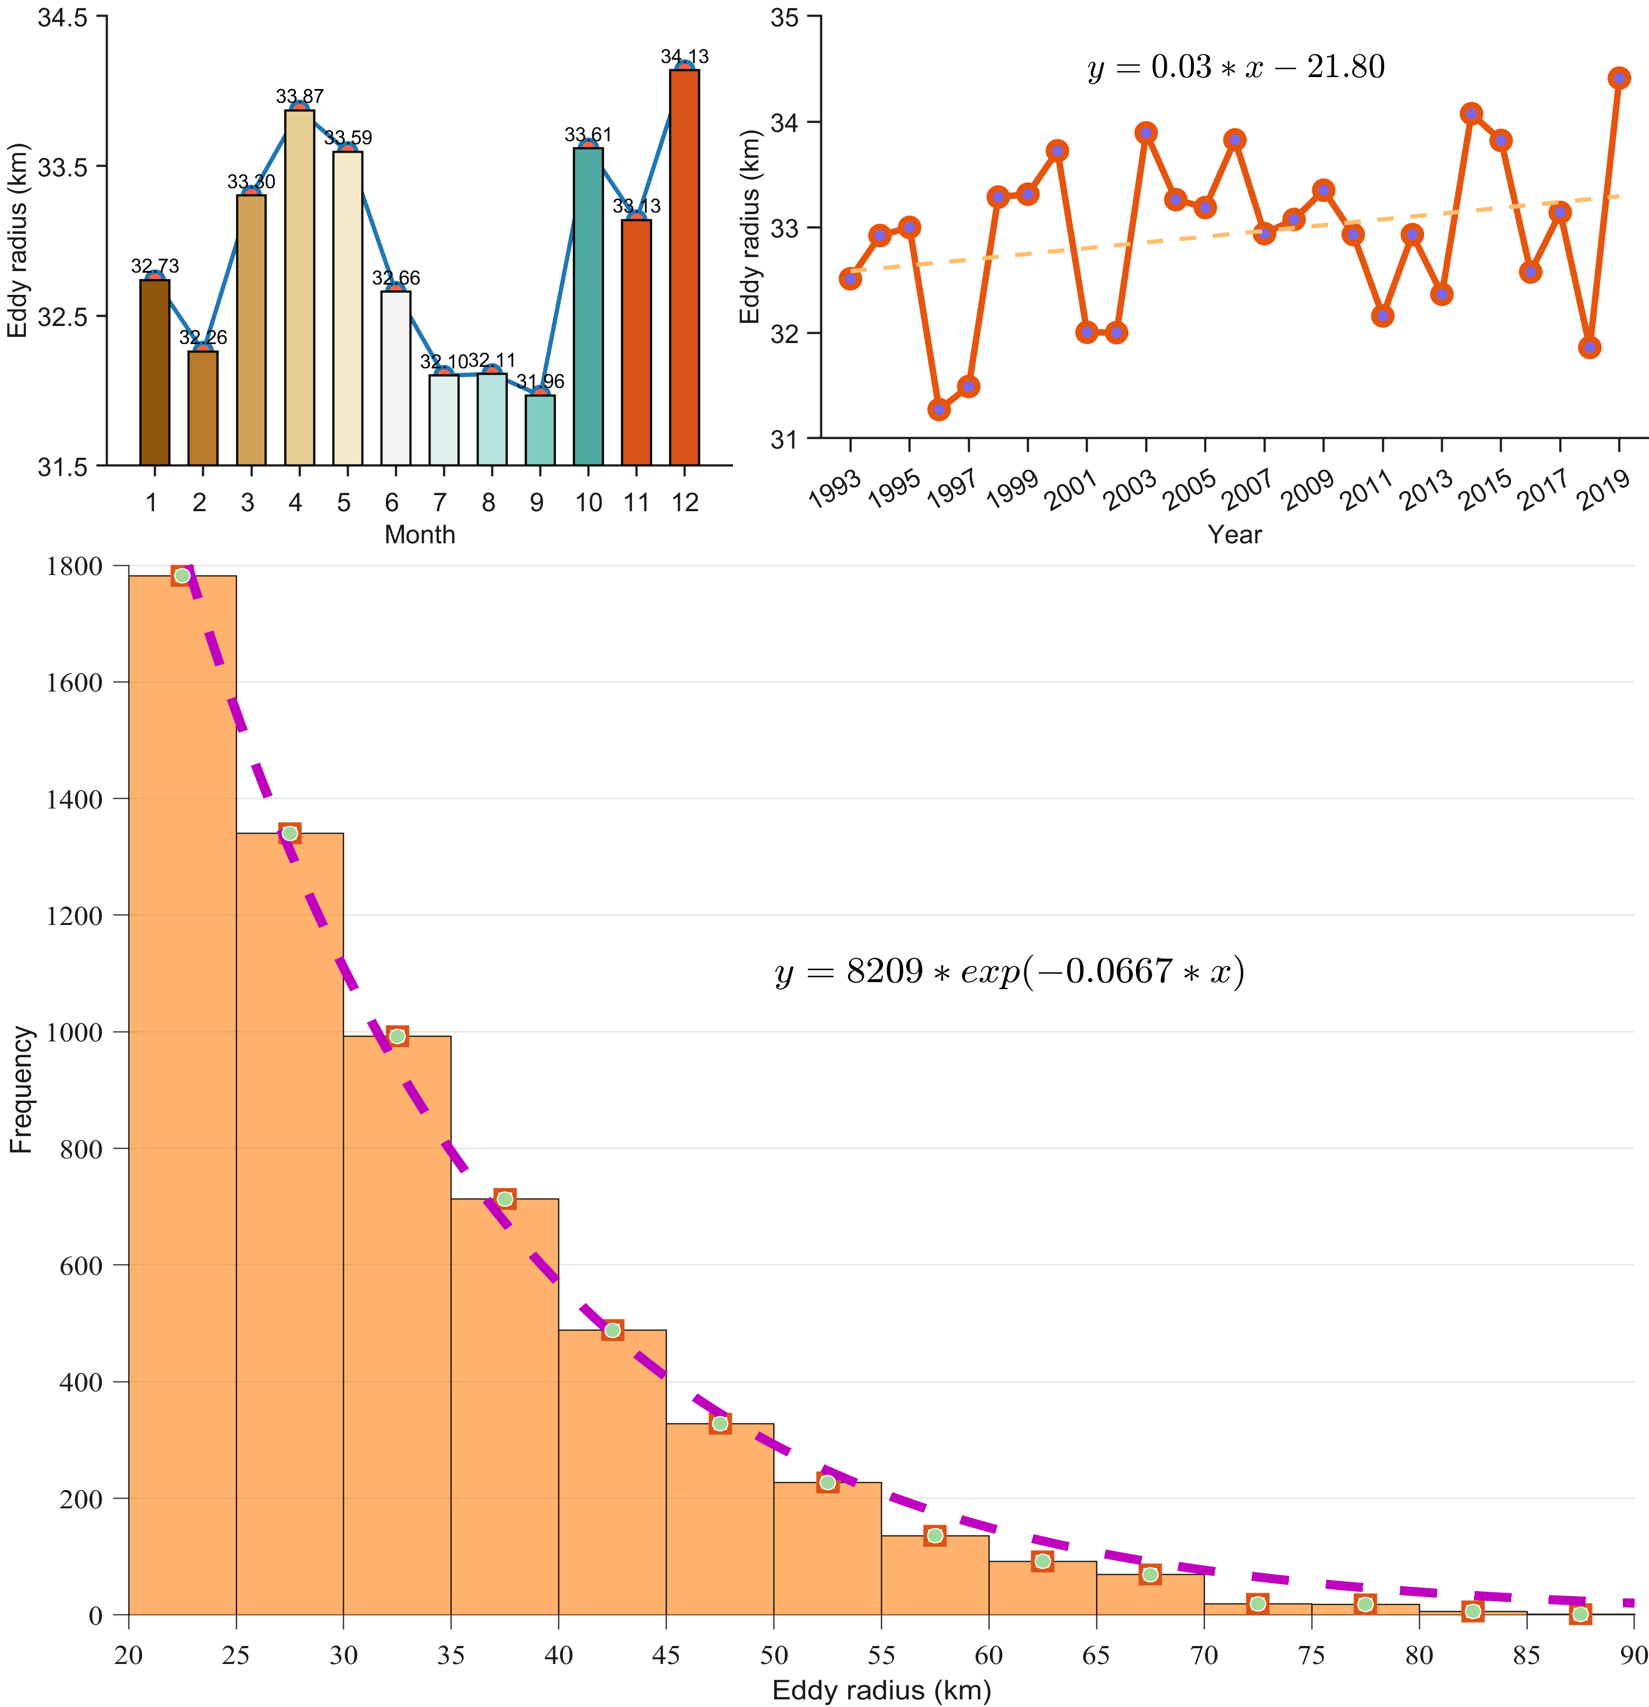
\includegraphics[width =15cm]{chapter/figure/eddy radius2.png}
    \caption{Eddy radius frequency distribution histogram}
    \label{Eddy radius map}
\end{figure}

The figure \ref{radius vs latitude} shows how eddy's radius changes with latitude. From the figure, we could learn that eddies in high latitudes would tend to have a smaller radius, and eddies in lower latitudes would have a larger radius. We also calculated the stretching ratio between the initial eddy area and the final eddy area and the result is shown in figure \ref{enlargement vs latitude}. We infer that eddy would have an inclination to be compressed during the coherent period and the ratio reduces to 0.85 from  $-55^\circ$ S to $-60^\circ $ S, which suggests that the LAVD method may not be so robust in high latitude.

\begin{figure}
    \centering
    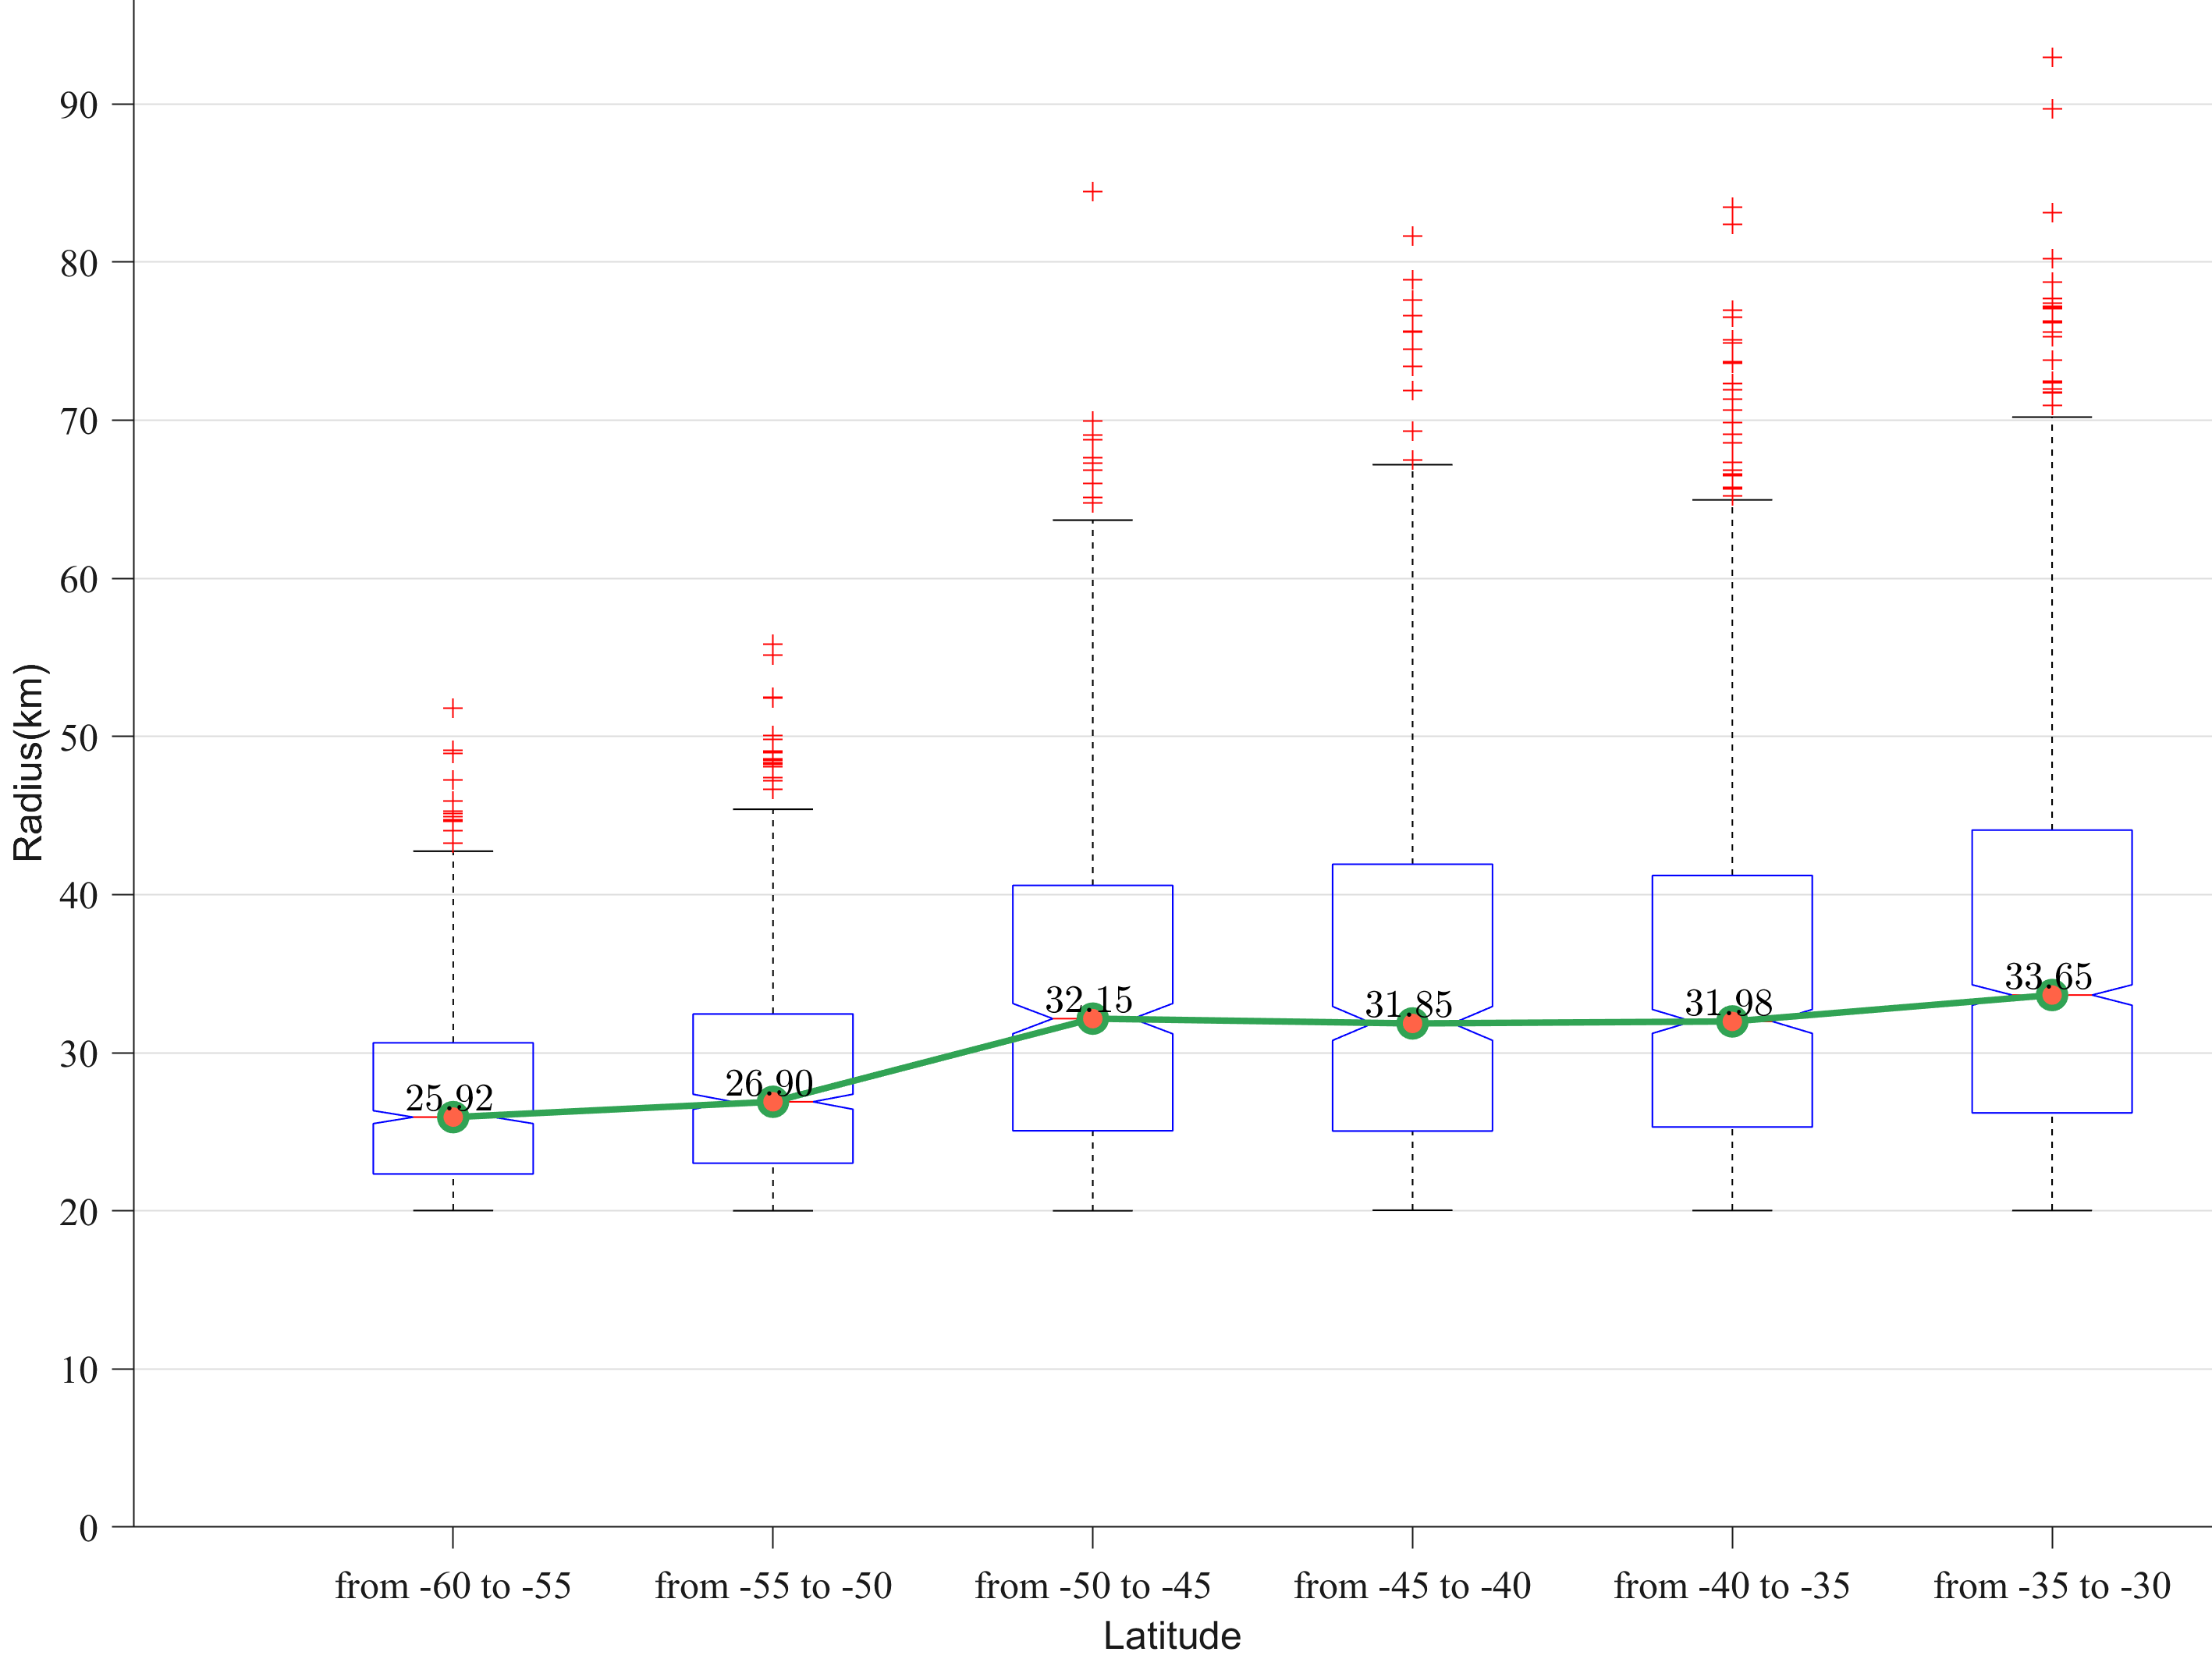
\includegraphics[width = 15cm]{chapter/figure/radius vs latitude.png}
    \caption{Relationship of vortex radius with latitude}
    \label{radius vs latitude}
\end{figure}

\begin{figure}
    \centering
    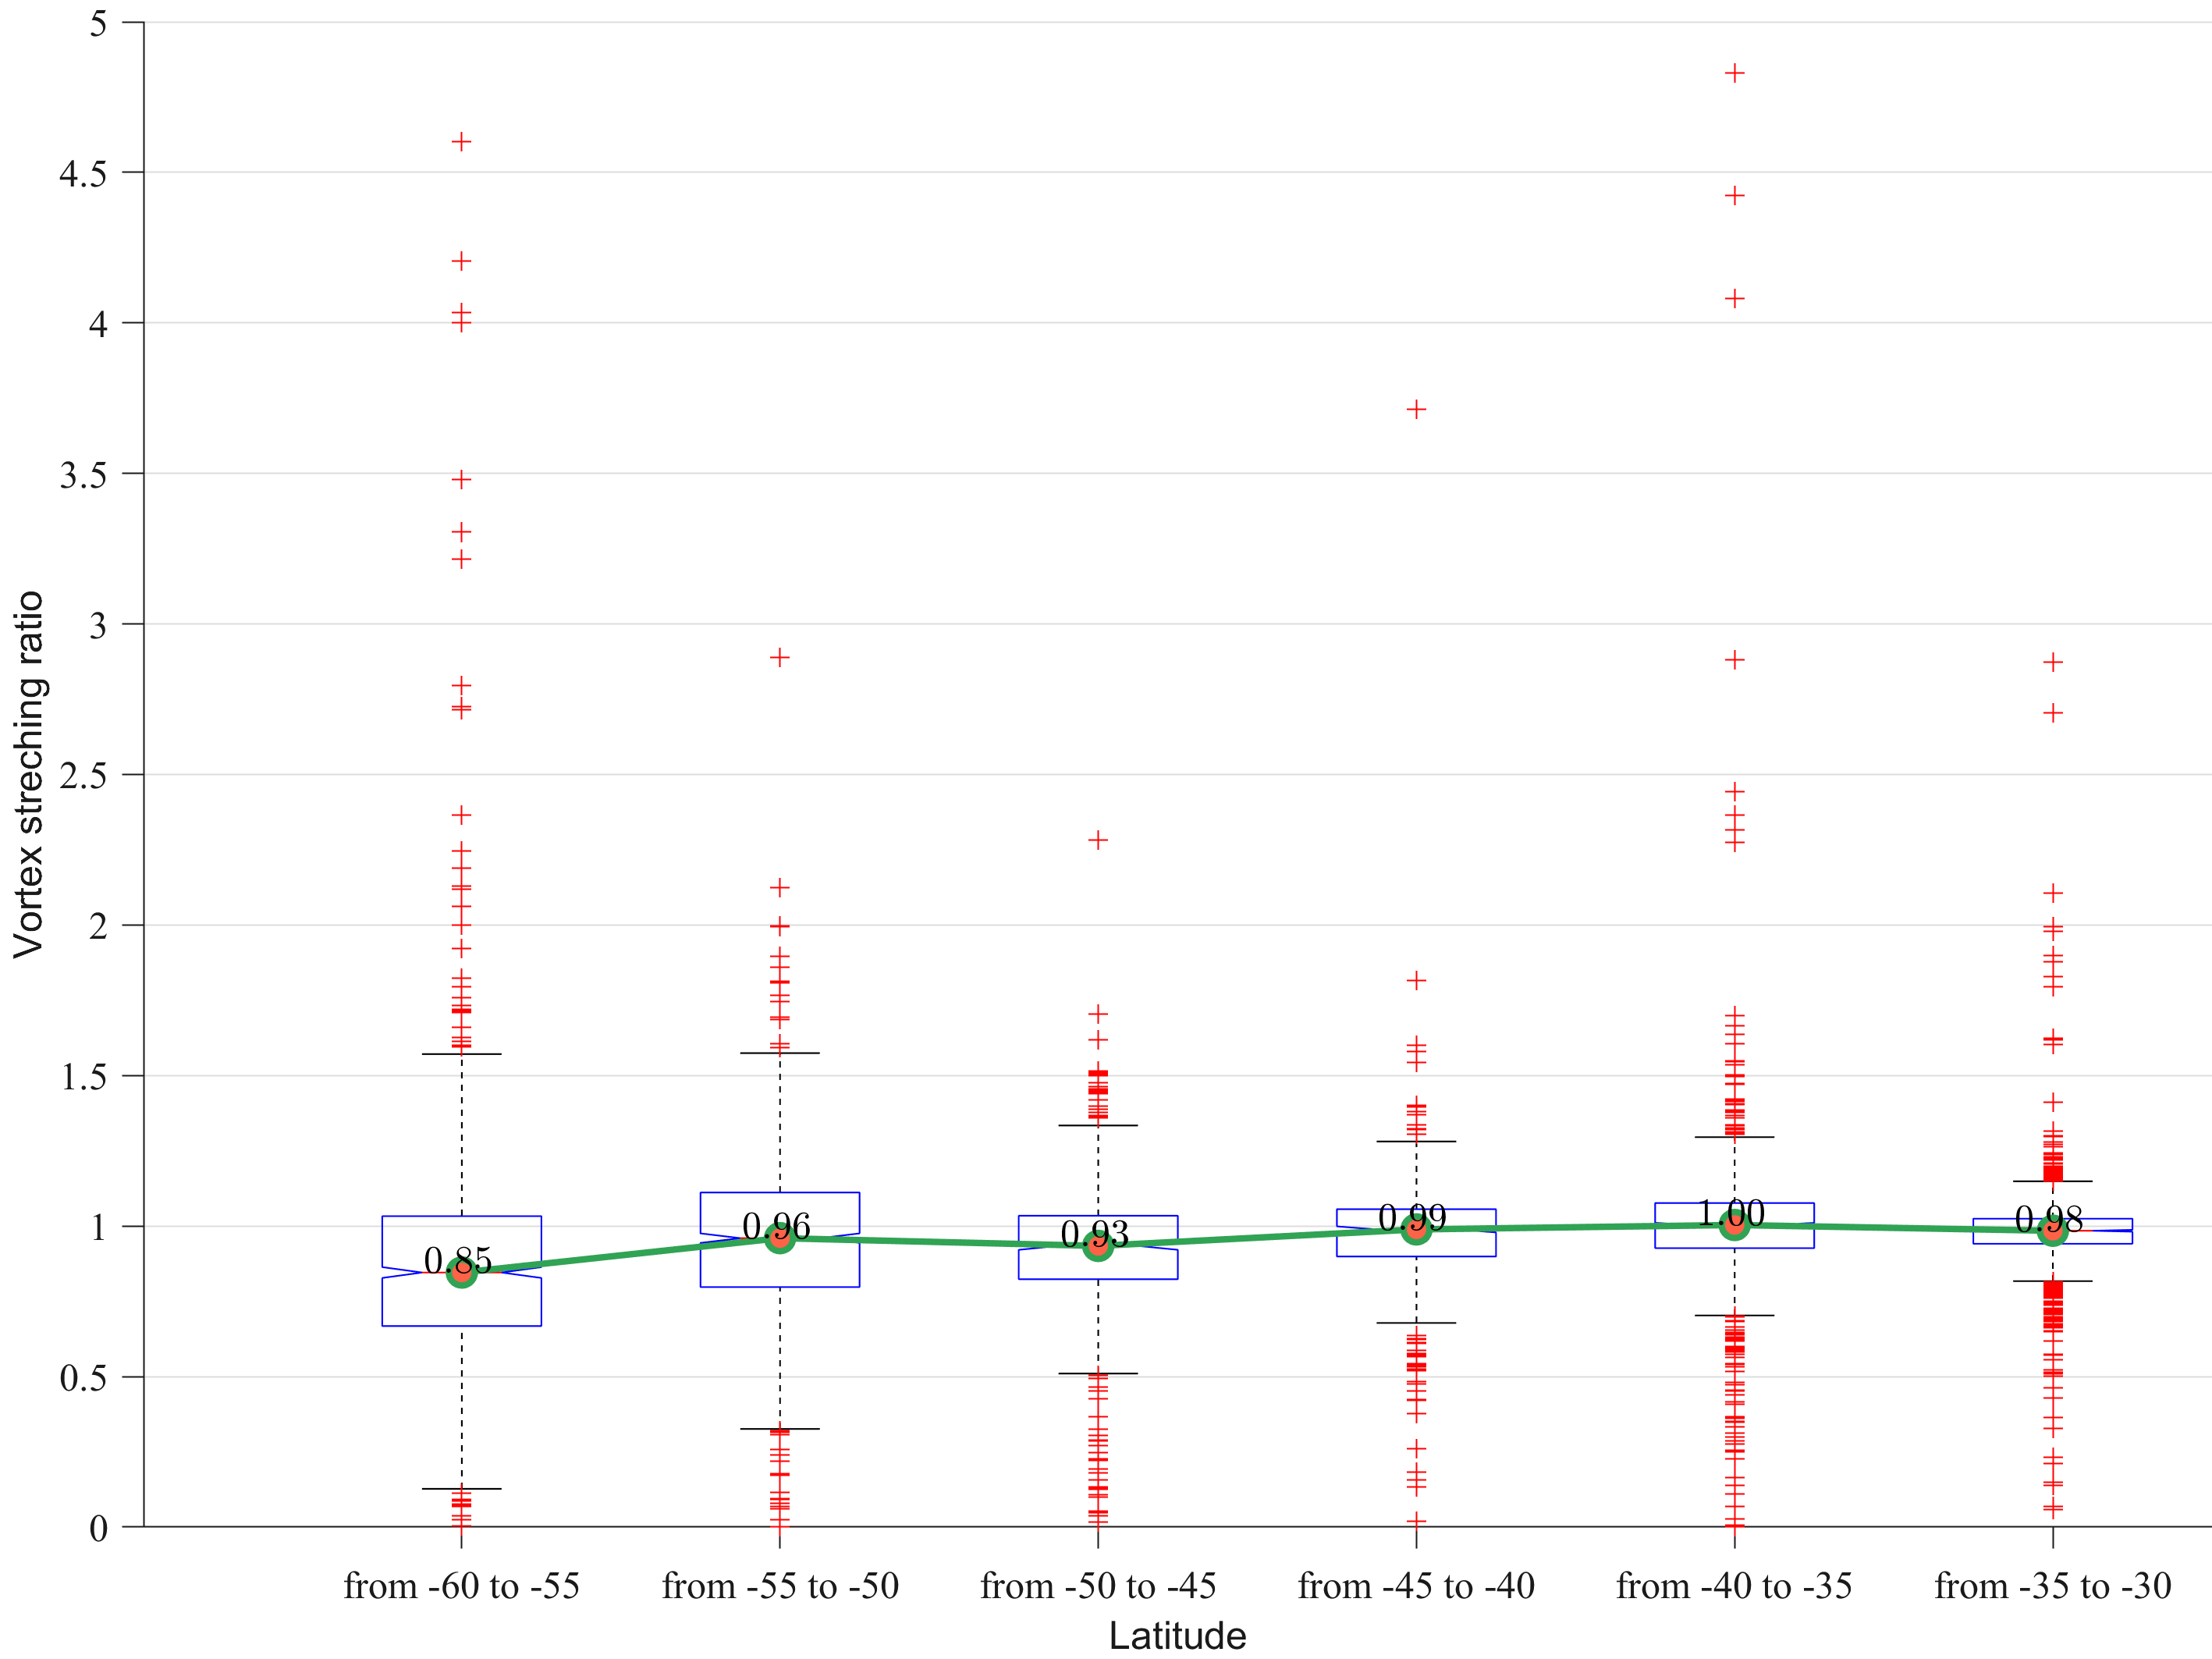
\includegraphics[width = 15cm]{chapter/figure/enlargement vs latitude.png}
    \caption{Relationship of vortex stretching ratio with latitude}
    \label{enlargement vs latitude}
\end{figure}

The figure \ref{velocity vs latitude} demonstrates how eddy propagates in the coherent period. The average propagation speed of the eddy is approximately 5km/day and eddies have the largest propagation speed (about 6.5 km/day) in the middle latitude ranging from $-50^\circ$ S to $-40^\circ$ S. However, the propagation speed will reduce to about 3.6 km/day in higher or lower latitude. There are many outliers for the vortex transport speed in the figure \ref{velocity vs latitude}, which implies the nonlinear effects and causes the vortex moves disorderly. What is more, in most of the cases, the eddy's zonal transport velocity outweighs its meridional component. As shown in figure \ref{Relationship of zonal and meridional velocity with latitude}, the maximum value of zonal velocity is 5.61 km/day near -45°S latitude while the maximum value of meridional velocity is 4.88 km/day at latitudes between -47°S and -50°S. They both show the trend of maximum at intermediate latitudes and decreasing at both low and high latitudes.


\begin{figure}
    \centering
    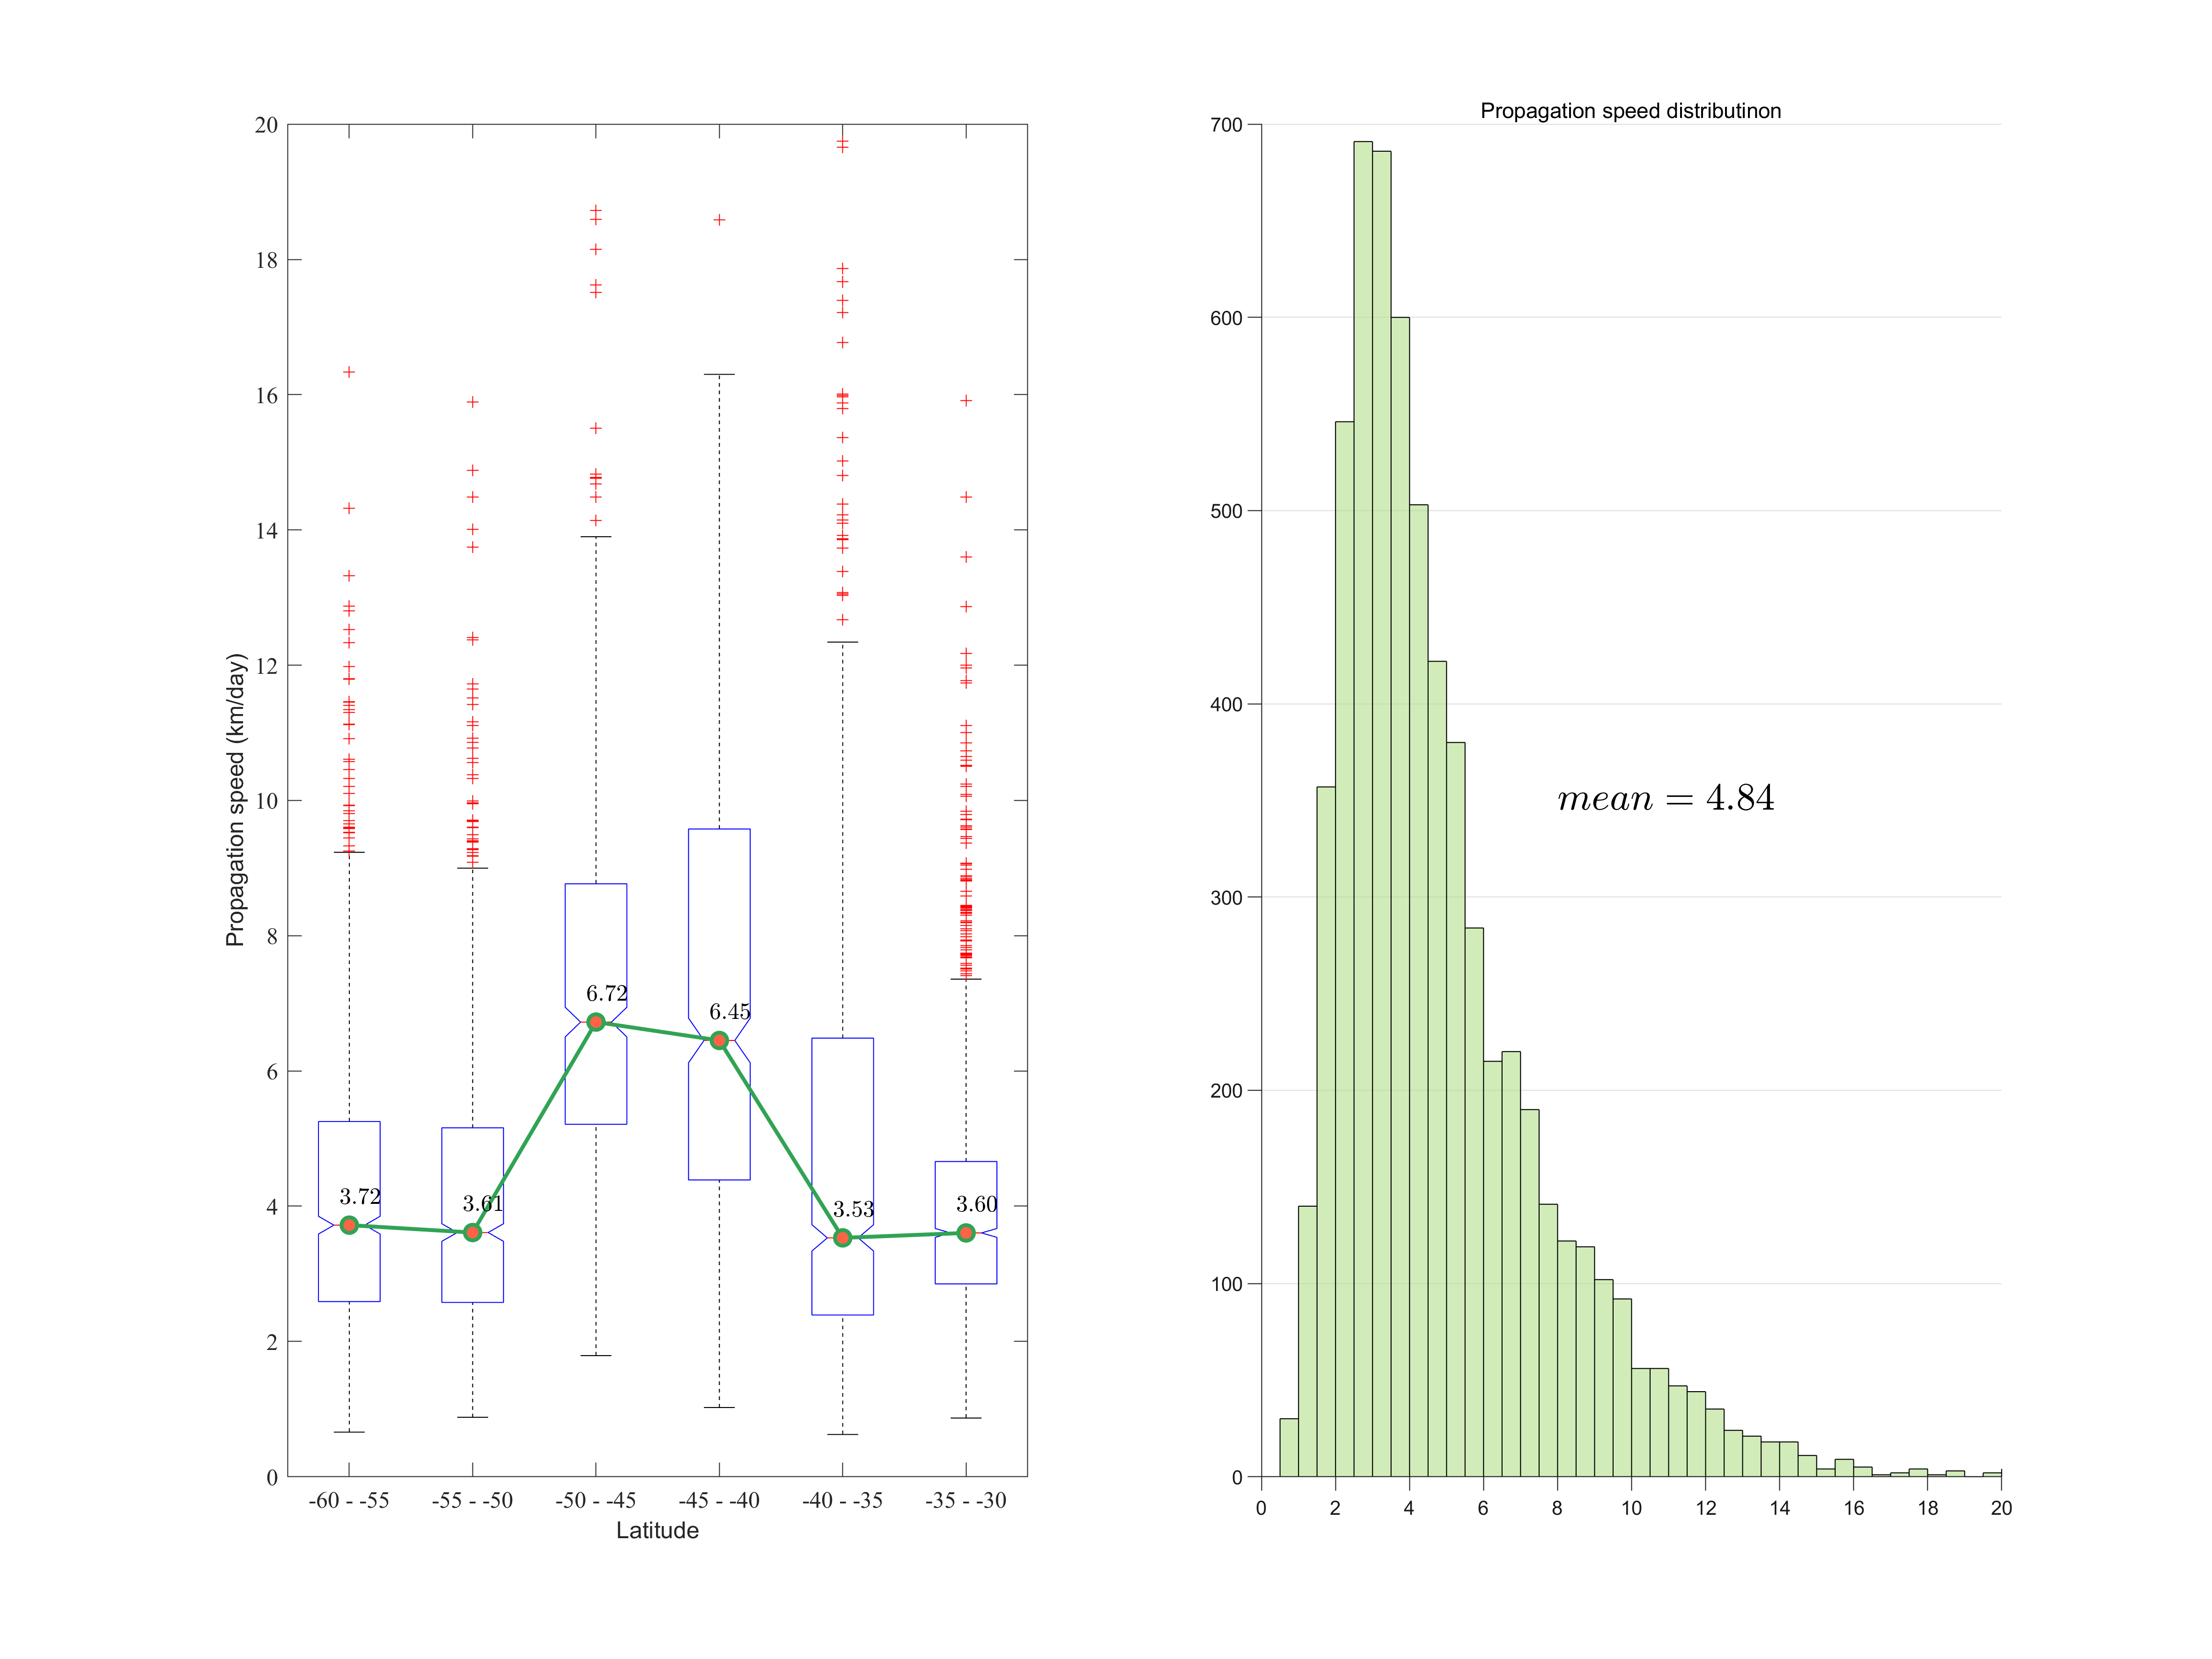
\includegraphics[width = 1.0\textwidth]{chapter/figure/velocity vs latitude.png}
    \caption{Relationship of eddy velocity (km) with latitude}
    \label{velocity vs latitude}
\end{figure}

\begin{figure}
    \centering
    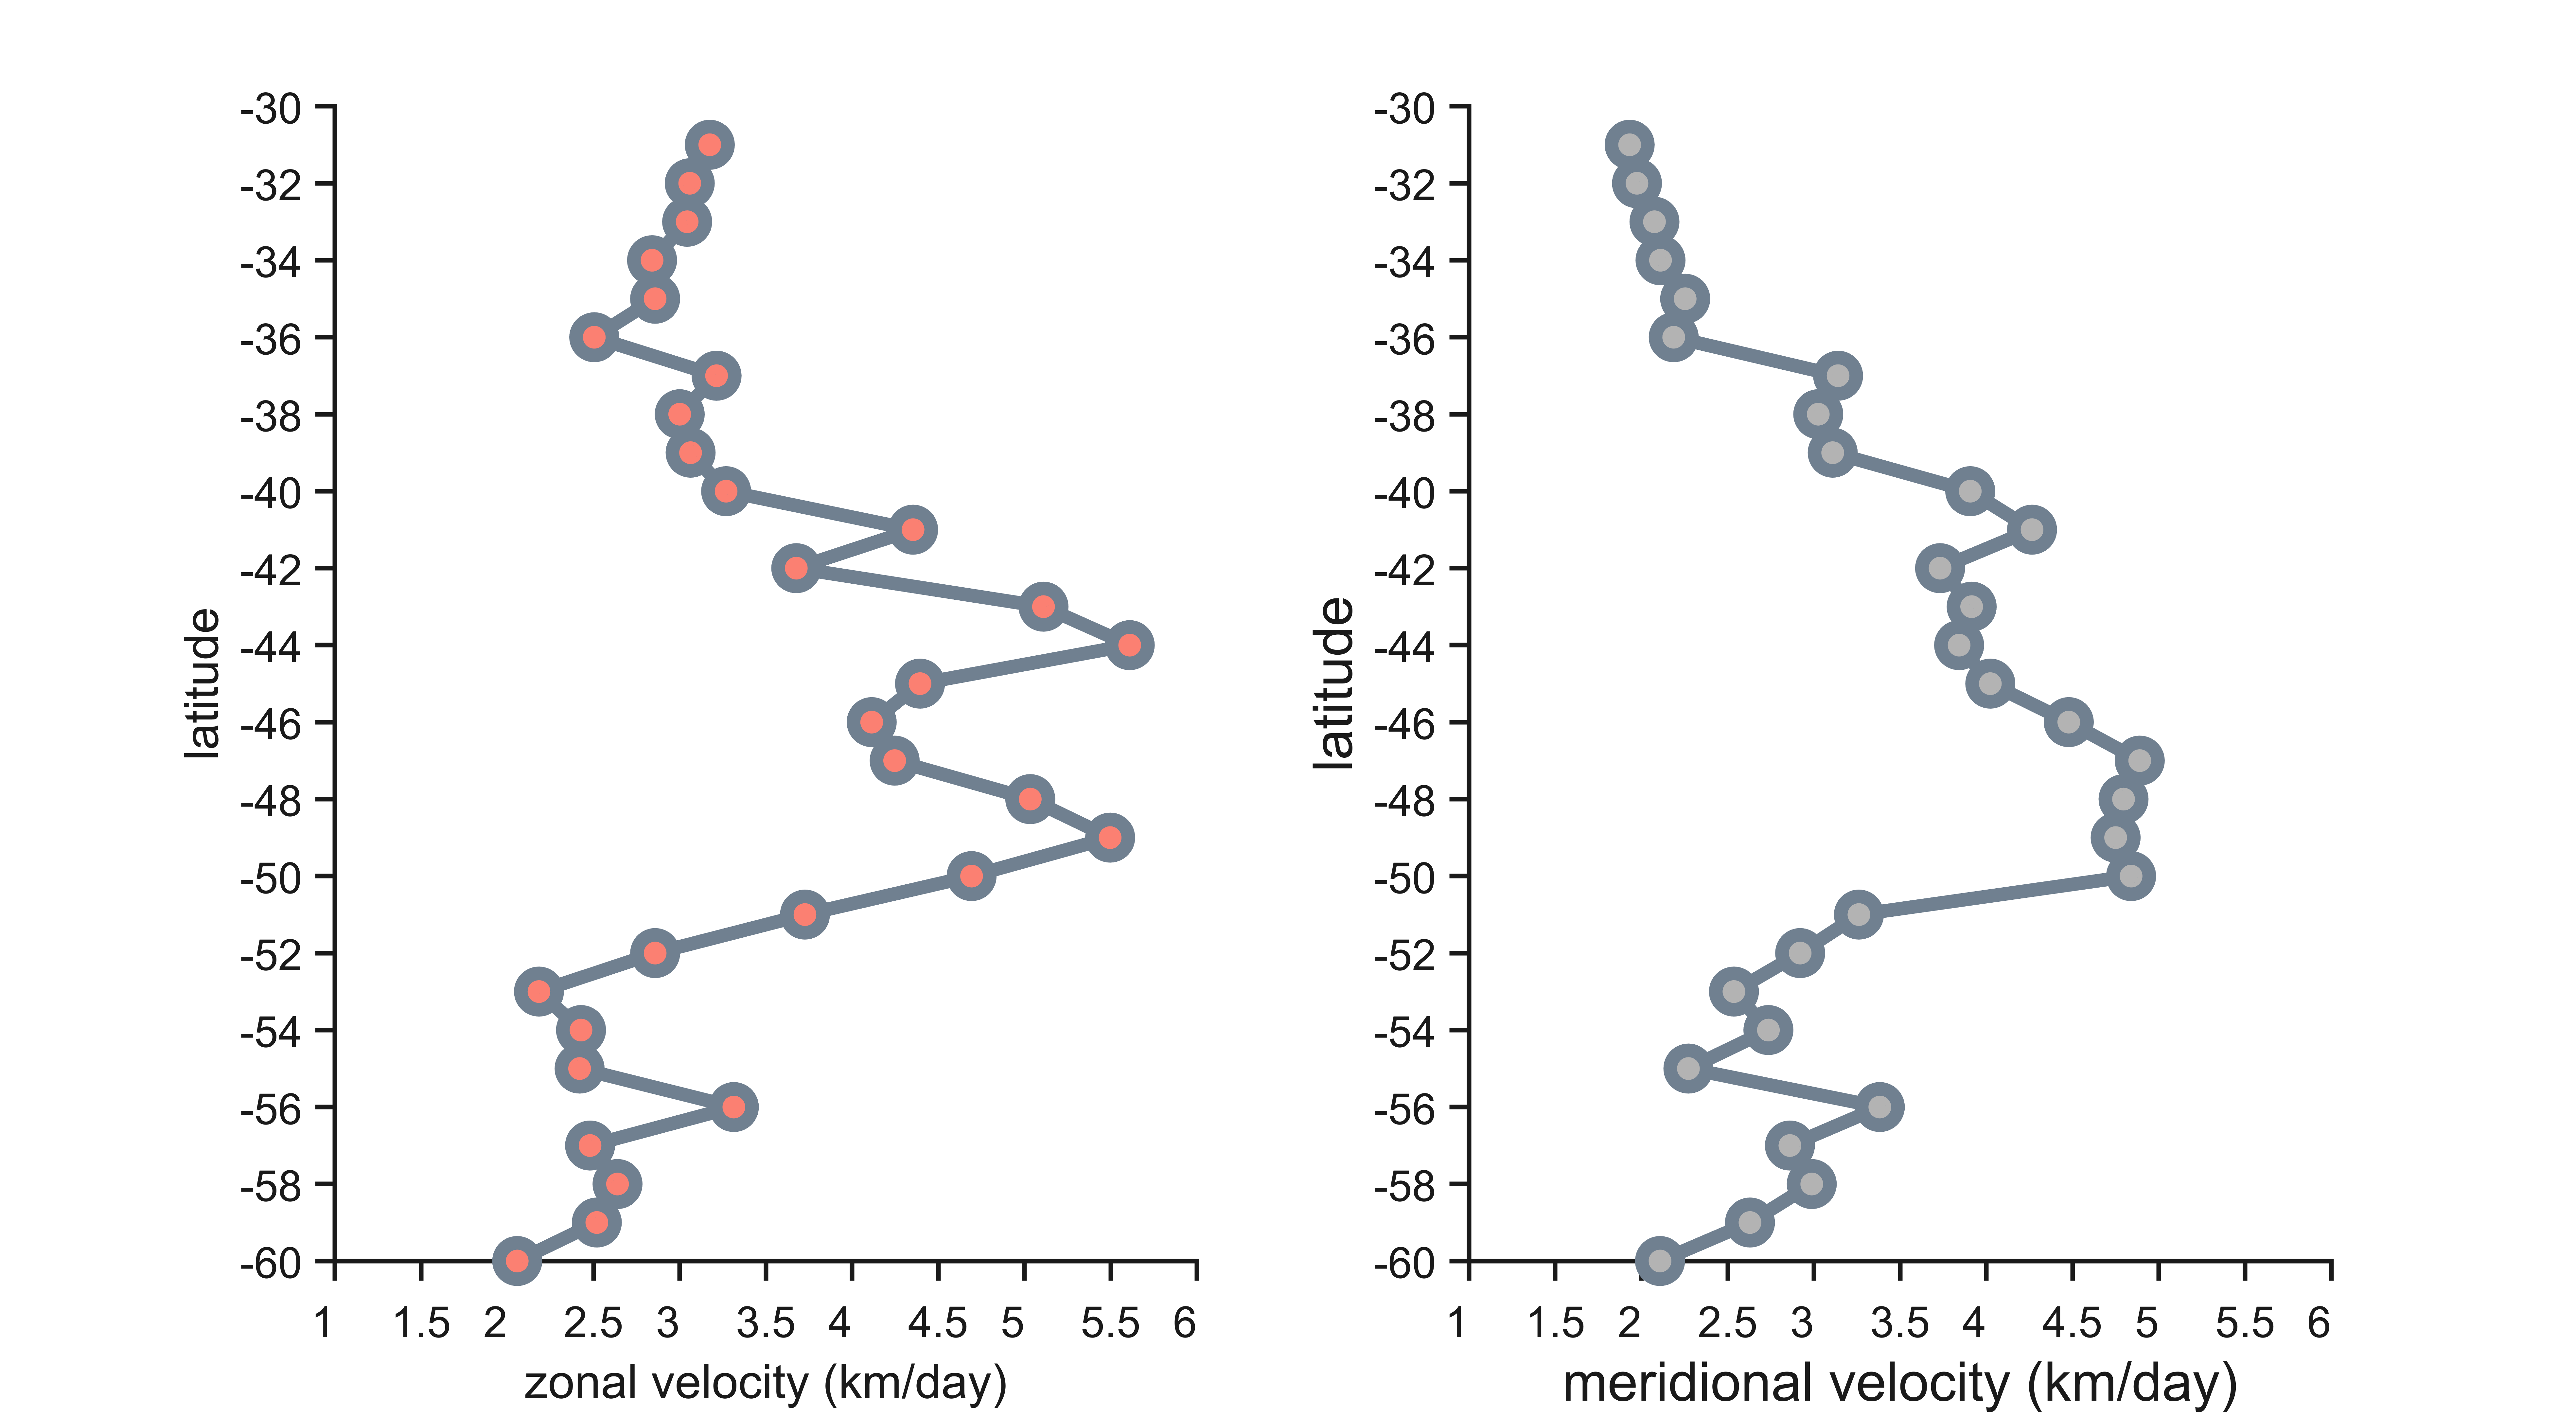
\includegraphics[width = 15cm]{chapter/figure/eddy velocity vs latitude.png}
    \caption{Relationship of zonal and meridional velocity with latitude}
    \label{Relationship of zonal and meridional velocity with latitude}
\end{figure}

The geographical distribution of eddies from 1993 to 2019 is given in the figure \ref{Eddy polarity map}. Among the 6212 vortices, 3336 of them are cyclonic eddies while 2876 of them are anti-cyclonic, which means that cyclonic vortices outweigh anticyclonic ones by about $15\%$. Along the southwest edge of the Argentine Basin, the majority of eddies were cyclonic eddies. Eddies distribute evenly in the Southern Ocean region, while there are more eddies in the northeast part of the Argentine Basin. There is a vortex "vacuum" zone in the center of the Argentine Basin, with only a few vortices remaining there. In the shallow water areas near South America Continent, we detected more anticyclonic vortices. There are few eddies detected in the coastal region since the deviation of altimeter data near the coastline is rather high due to the influence of tides and coastal waves. In the water regions connecting the Southern Ocean and Argentine Basin, eddies distribute in a striped pattern.

\begin{figure}
    \centering
    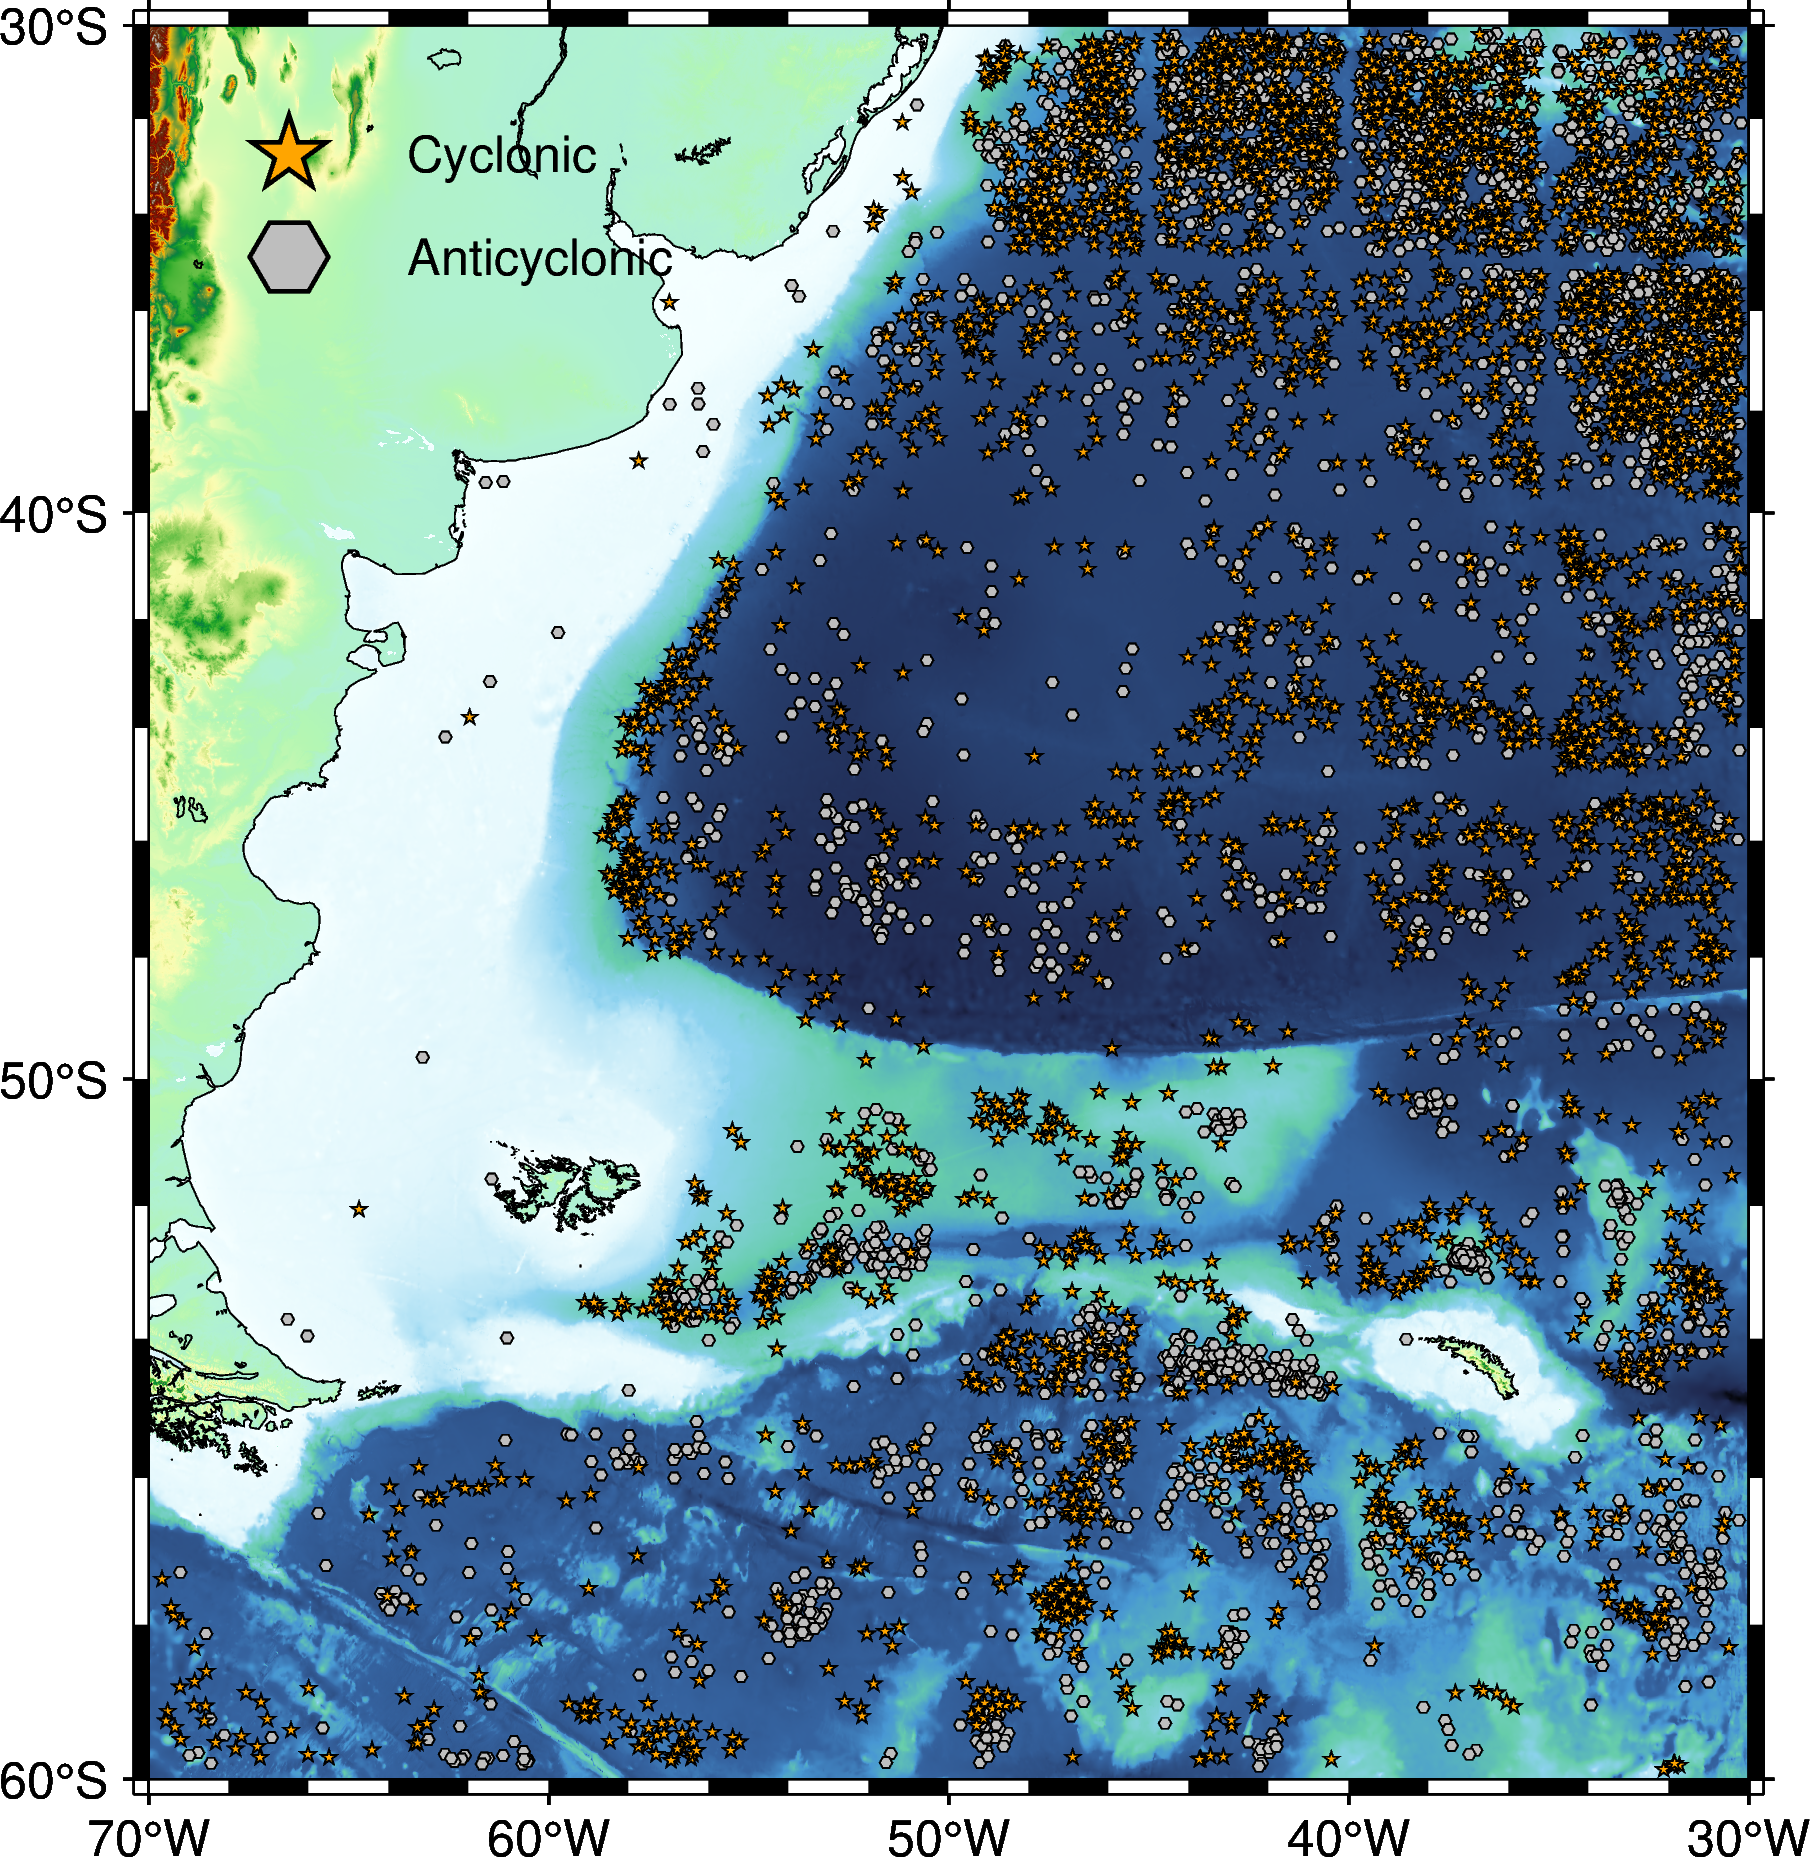
\includegraphics[width = 15cm]{chapter/figure/eddy polarity map.png}
    \caption{Eddy polarity distribution map}
    \label{Eddy polarity map}
\end{figure}

The figure \ref{eddy number vs Polarity} shows annual variation and monthly variation of eddy number and vortex radius of cyclonic and anti-cyclonic eddies. Anti-cyclonic eddies have distinct seasonal variations while seasonal number differences of cyclonic eddies are small. In all months, the number of cyclonic vortices is higher than the anti-cyclonic ones. The average number of anti-cyclonic eddies appearing in June is 7.59, which is the lowest in all months. Anti-cyclonic eddy number reaches the minimum value in winter and it increases slowly and reaches a maximum in winter. Annual variation characteristics of vortex numbers tell us that in most of the years, cyclonic eddy numbers outweigh anti-cyclonic ones while the opposite rule was observed in 1995 and 1996. An average of 124 cyclonic vortices and 107 anti-cyclonic eddies are generated each year. Both the number of cyclonic eddies and anti-cyclonic eddies would increase, and the increasing trend of cyclonic eddies is more obvious. The maximum number of annual cyclonic eddies found in the Argentine Basin is 168 in 2019 while the maximum number of annual anti-cyclonic eddies is 133 in 2006.

\begin{figure}
    \centering
    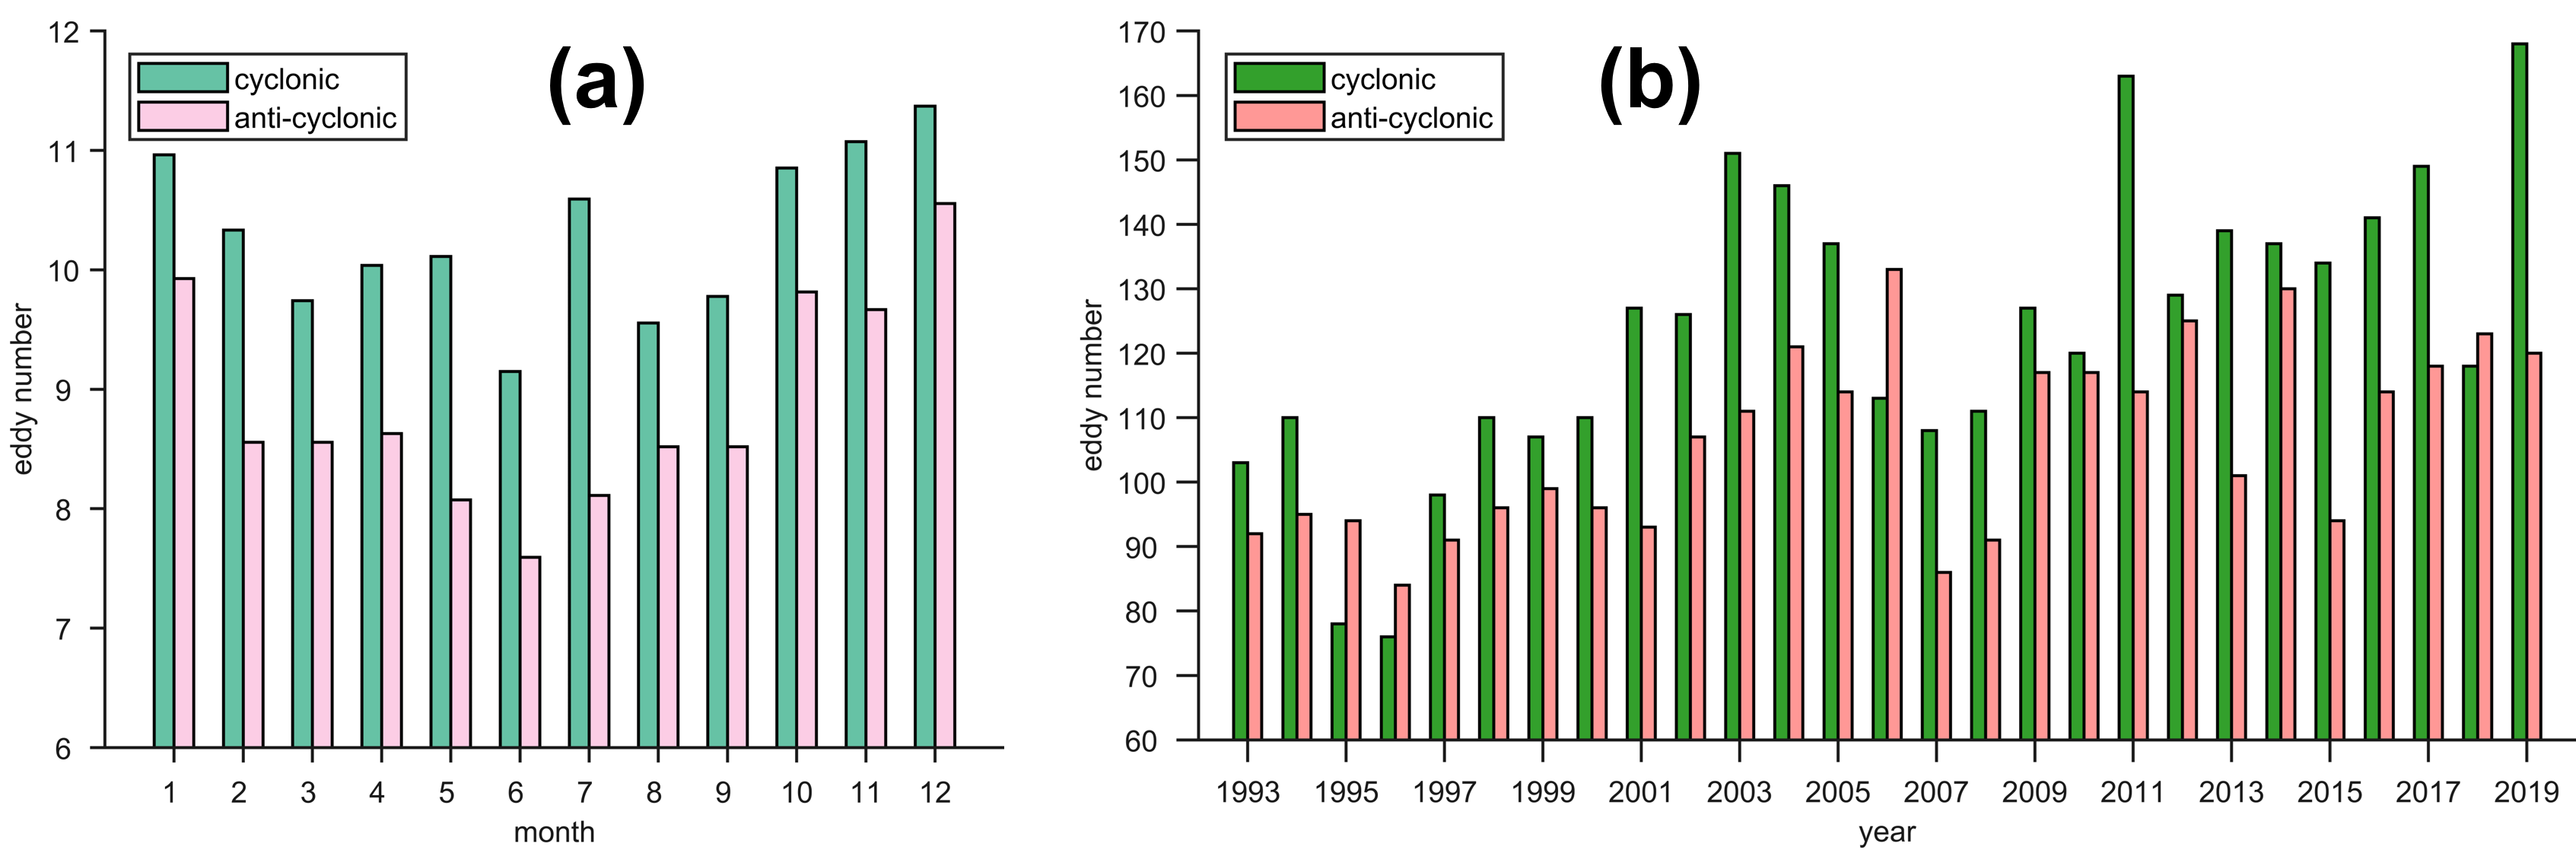
\includegraphics[width = 15cm]{chapter/figure/eddy number vs Polarity.png}
    \caption{Monthly and annual patterns of eddy number of different polarities}
    \label{eddy number vs Polarity}
\end{figure}

Figure \ref{eddy radius vs type} shows how vortex polarity affects vortex size. Before 2010, the diameter of the anticyclonic vortex was more extensive than that of the cyclonic vortex. Since 2007, the radius of cyclonic vortex began to grow and has become bigger than anti-cyclonic ones. From the figure, we could learn that different types of eddies have different seasonal patterns. The average monthly minimum radius of cyclonic eddies is 31.52 km in September while the minimum monthly radius of anti-cyclonic vortices is about 32 km in June. They both show maximum value in December.

\begin{figure}
    \centering
    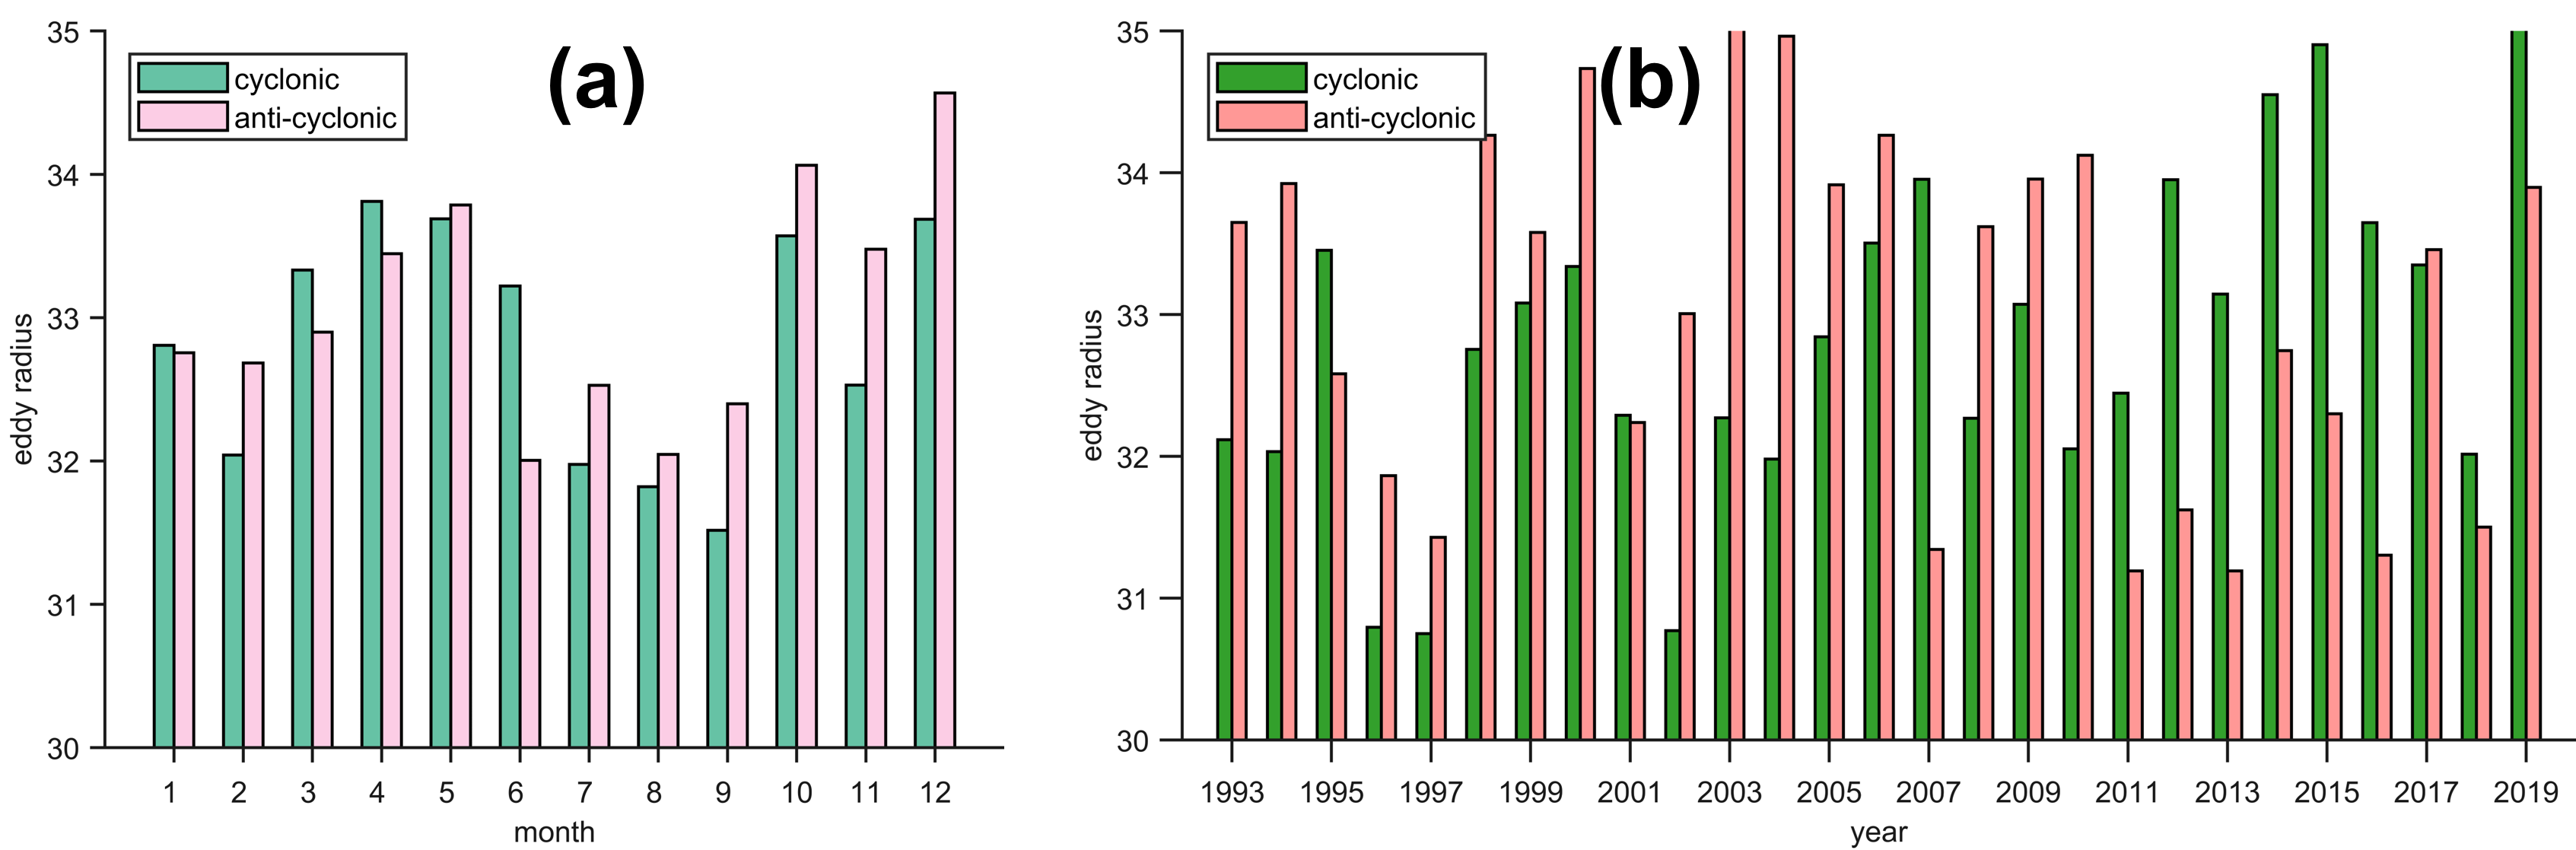
\includegraphics[width = 15cm]{chapter/figure/eddy radius vs type.png}
    \caption{Monthly and annual patterns of eddy radius of different polarities}
    \label{eddy radius vs type}
\end{figure}

In Figure \ref{eddy classification map_SNWE2}, we compared eddies' initial position and final position from 1993 to 2019 and the figure shows the direction of eddy propagation. About $59\%$ of the eddies would travel northward, and only $41\%$ would travel southward. Anticyclonic vortices are more inclined to transport to the poles. In the east-west direction, about $63\%$ of the eddies travel westward, and only $37\%$ of them travel to the east.

From the map, we could learn that even in the northern part of the Argentine Basin which is affected by the southward Brazil Current, most of the eddies would tend to travel northward, which suggests an opposite direction of the mean flow and eddy flow. Along the border connecting the shallow water region and Argentine Basin, we could learn that eddies in the northern part of the border have an inclination to travel southward and eddies in the southern part have a trend to travel northward. This is coincident with the southward Brazil Current and northward Malvinas Current. In the middle of the Argentine Basin, eddies' travel pattern agrees with the Zapiola Anticyclone.

In the Southern Ocean region, most of the observed eddies travel eastward because of the Antarctic Circumpolar Current. On the northern part of the Argentine Basin, the majority of the eddies propagate westward.
In the center of the basin, because of the Argentine Gyre and branch of the Brazil Current, we could see that at the southern edge of the basin, eddies would tend to move eastward while eddies would move to the west in the middle of the basin.

\begin{figure}
    \centering
    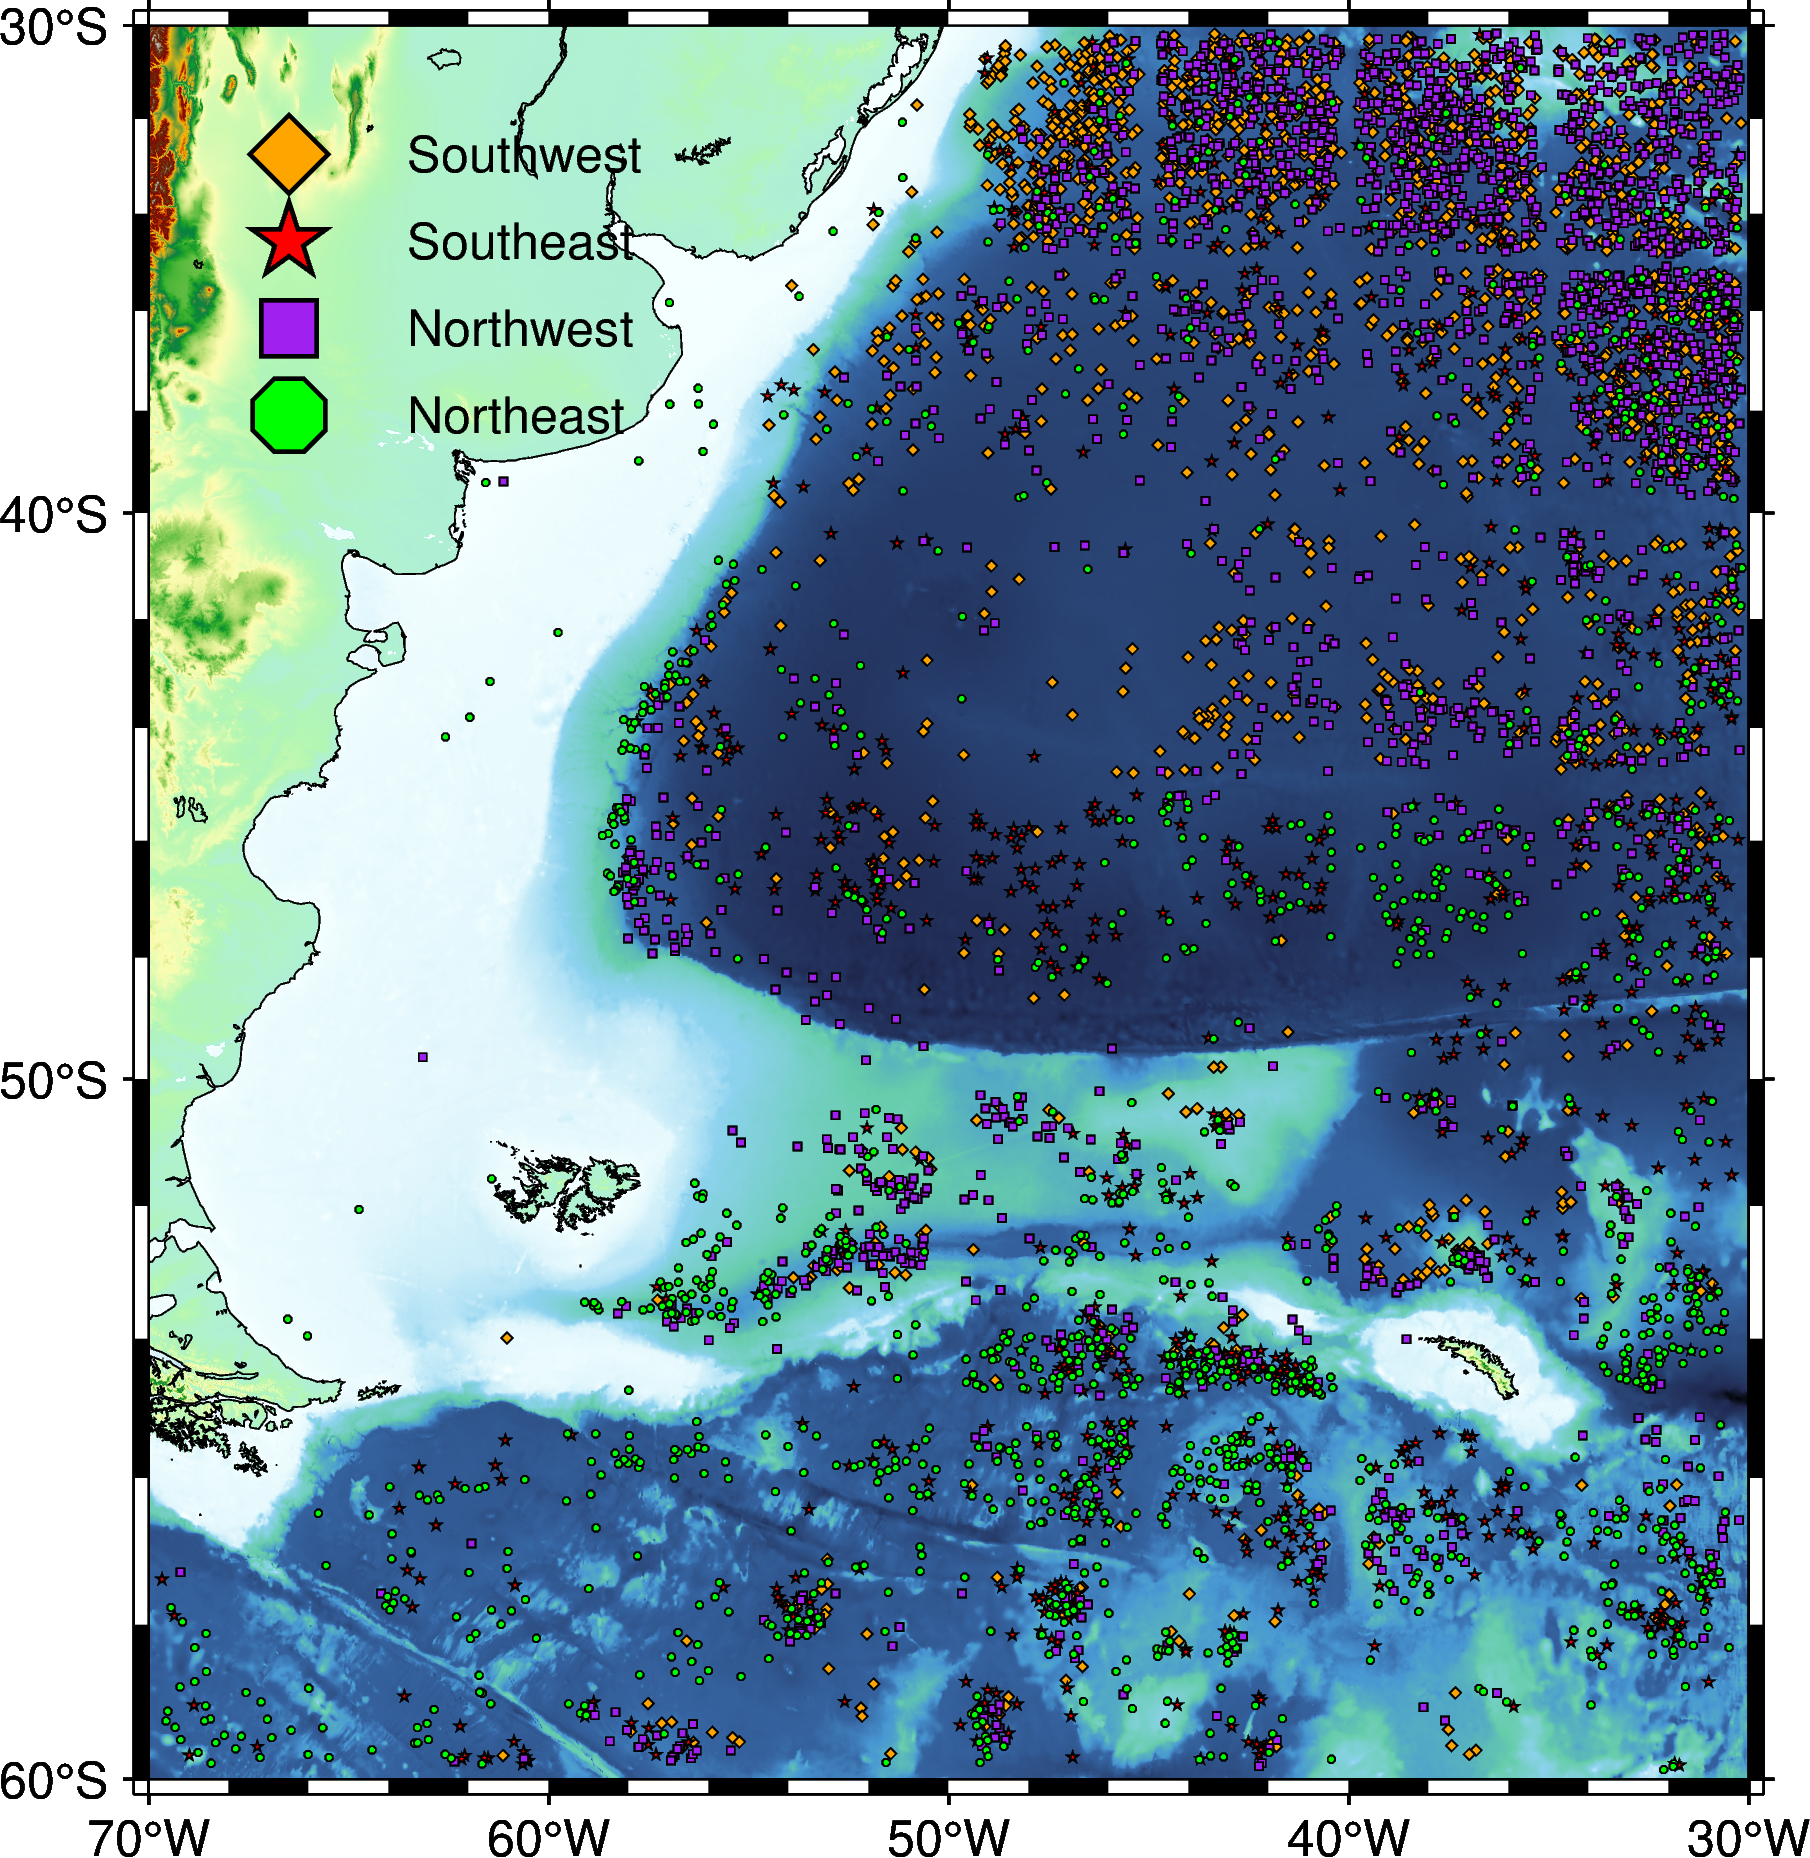
\includegraphics[width = 15cm]{chapter/figure/eddy classification map_SNWE2.png}
    \caption{Eddy travel direction map}
    \label{eddy classification map_SNWE2}
\end{figure}

Figure \ref{some vortex examples} shows some cases study of the  eddies transport path. As shown in section (a) of figure \ref{some vortex examples}, a cyclonic eddy propagates westward in the center of the Argentine Basin. Section b shows an anti-cyclonic eddy on the southern border of the basin and its travel direction is to the southeast. In Section C of the figure, one cyclonic eddy near South Georgia and the South Sandwich Islands goes north and it lost its coherence strongly during the last ten days of transport. Section d of the figure depicts a typical vortex going southward along the South American continental slope, the direction of which is the same as the mean flow thus, a considerable number of vortices are also transported this way.


\begin{figure}
    \centering
    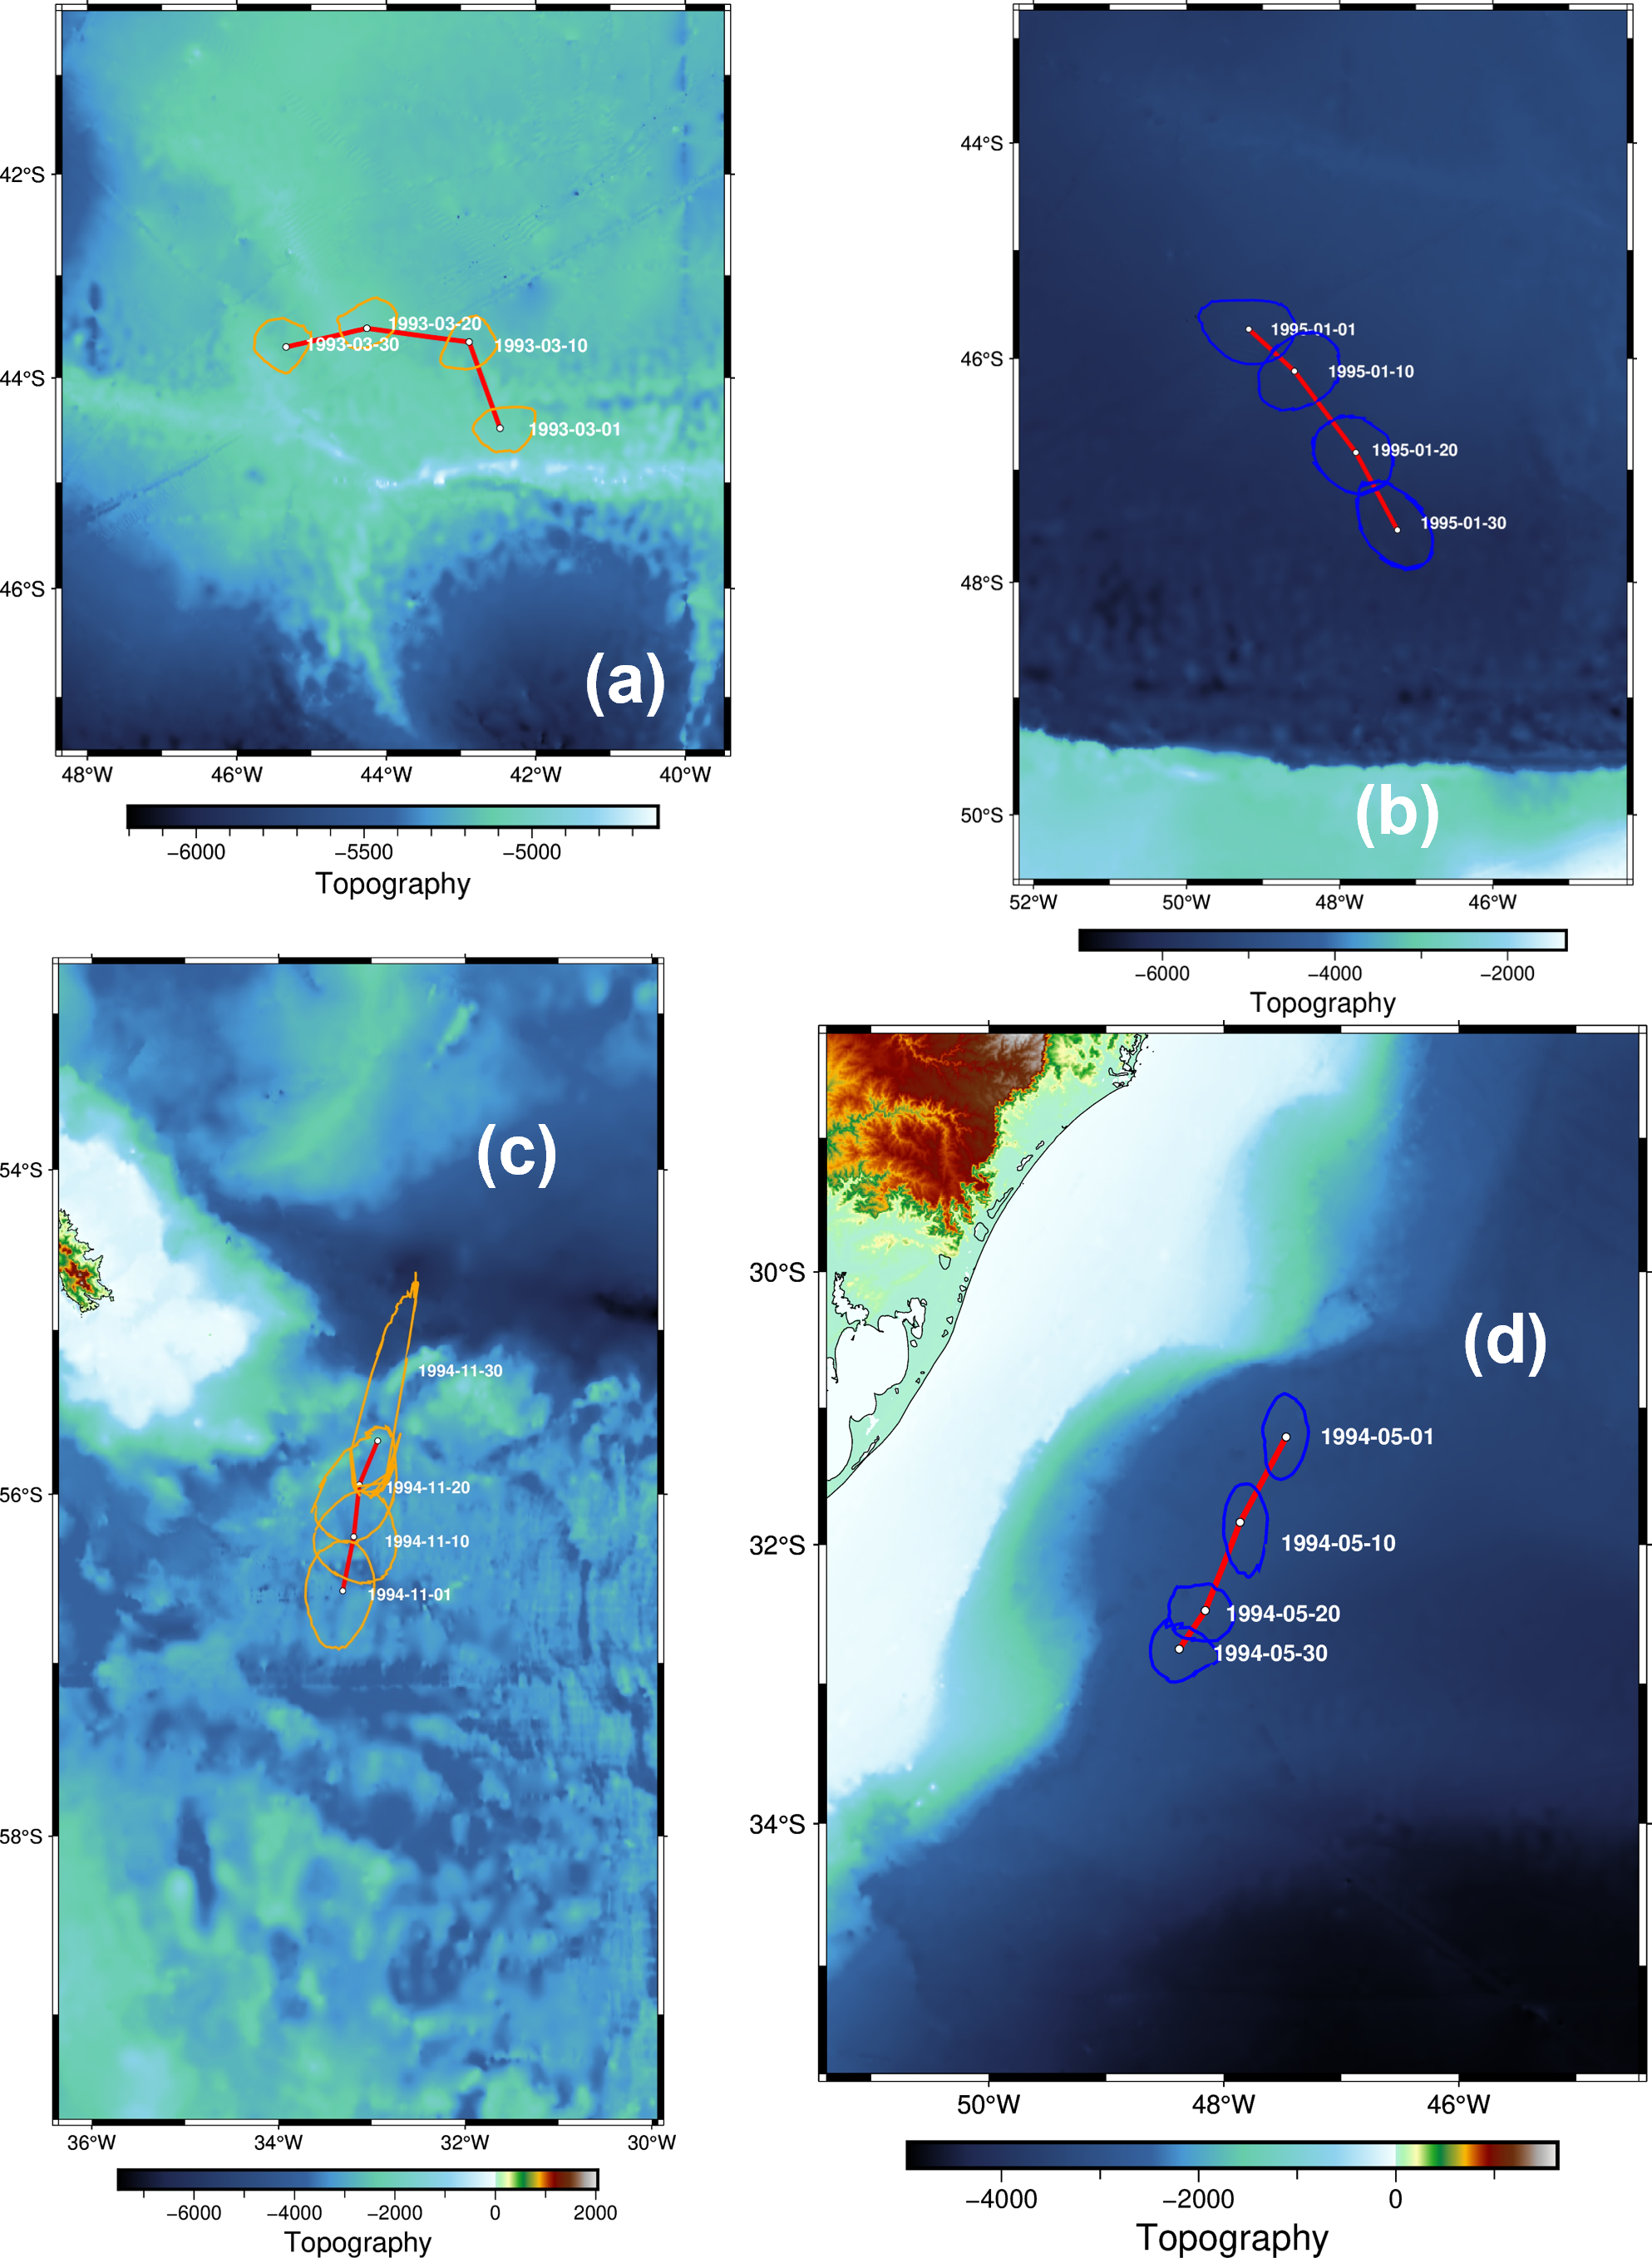
\includegraphics[width = 0.9\textwidth]{chapter/figure/eddy map.png}
    \caption{Some vortex examples (orange for cyclonic eddy and blue for anti-cyclonic eddy)}
    \label{some vortex examples}
\end{figure}

% \section{Eddies morphology}

\section{Eddies coherence time}

In Chapter \ref{Eddies statistics}, we set the coherent time of 30-day and detect 6212 coherent eddies in the study period from 1993 to 2019. However, the properties of the coherent eddy are affected by the selection of time interval to a large extent \cite{xia2022global,vortmeyer2016detecting}.

In the context of the Eulerian detection method (SSHA), the vortex life cycle is defined as the time period of the process of a vortex from birth to death \cite{mccoy2020global,andrade2020genesis}.
According to the previous research, the life cycle of a vortex varies from 4 weeks to  16 weeks and the average life cycle is about 8-9 weeks.

The result is shown in figure \ref{eddy coherent}. From the figure, we could learn that there is a rapid decrease in eddy number when the coherent period is less than 90 days, but the trend slows down after 90 days, which means that an eddy with a life cycle larger than 90 days would tend to survive longer. We could also conclude that eddies with a coherent period of 90 days have the largest radius which suggests that an eddy with a larger radius, magnitude, and intensity will survive longer. 60-day eddies' radius is smaller than 30-day eddies' and 120-day eddies' radius is smaller than 60-day eddies', which 
shows that the time period has an impact on vortex coherence and if we track the eddy exceeding the period $\Delta t$, the outer part of the eddies would be deformed, stretched into filaments, and finally lose coherence.

From figure \ref{eddy type proportion}, we could learn that anticyclonic eddies tend to have larger coherent time. When the coherence period is 30-day, anti-cyclonic eddies only occupy $46\%$ of the total eddy number; while the proportion raise up to $64\%$ when the coherent interval is 120-day.

\begin{figure}[htbp]
    \centering
    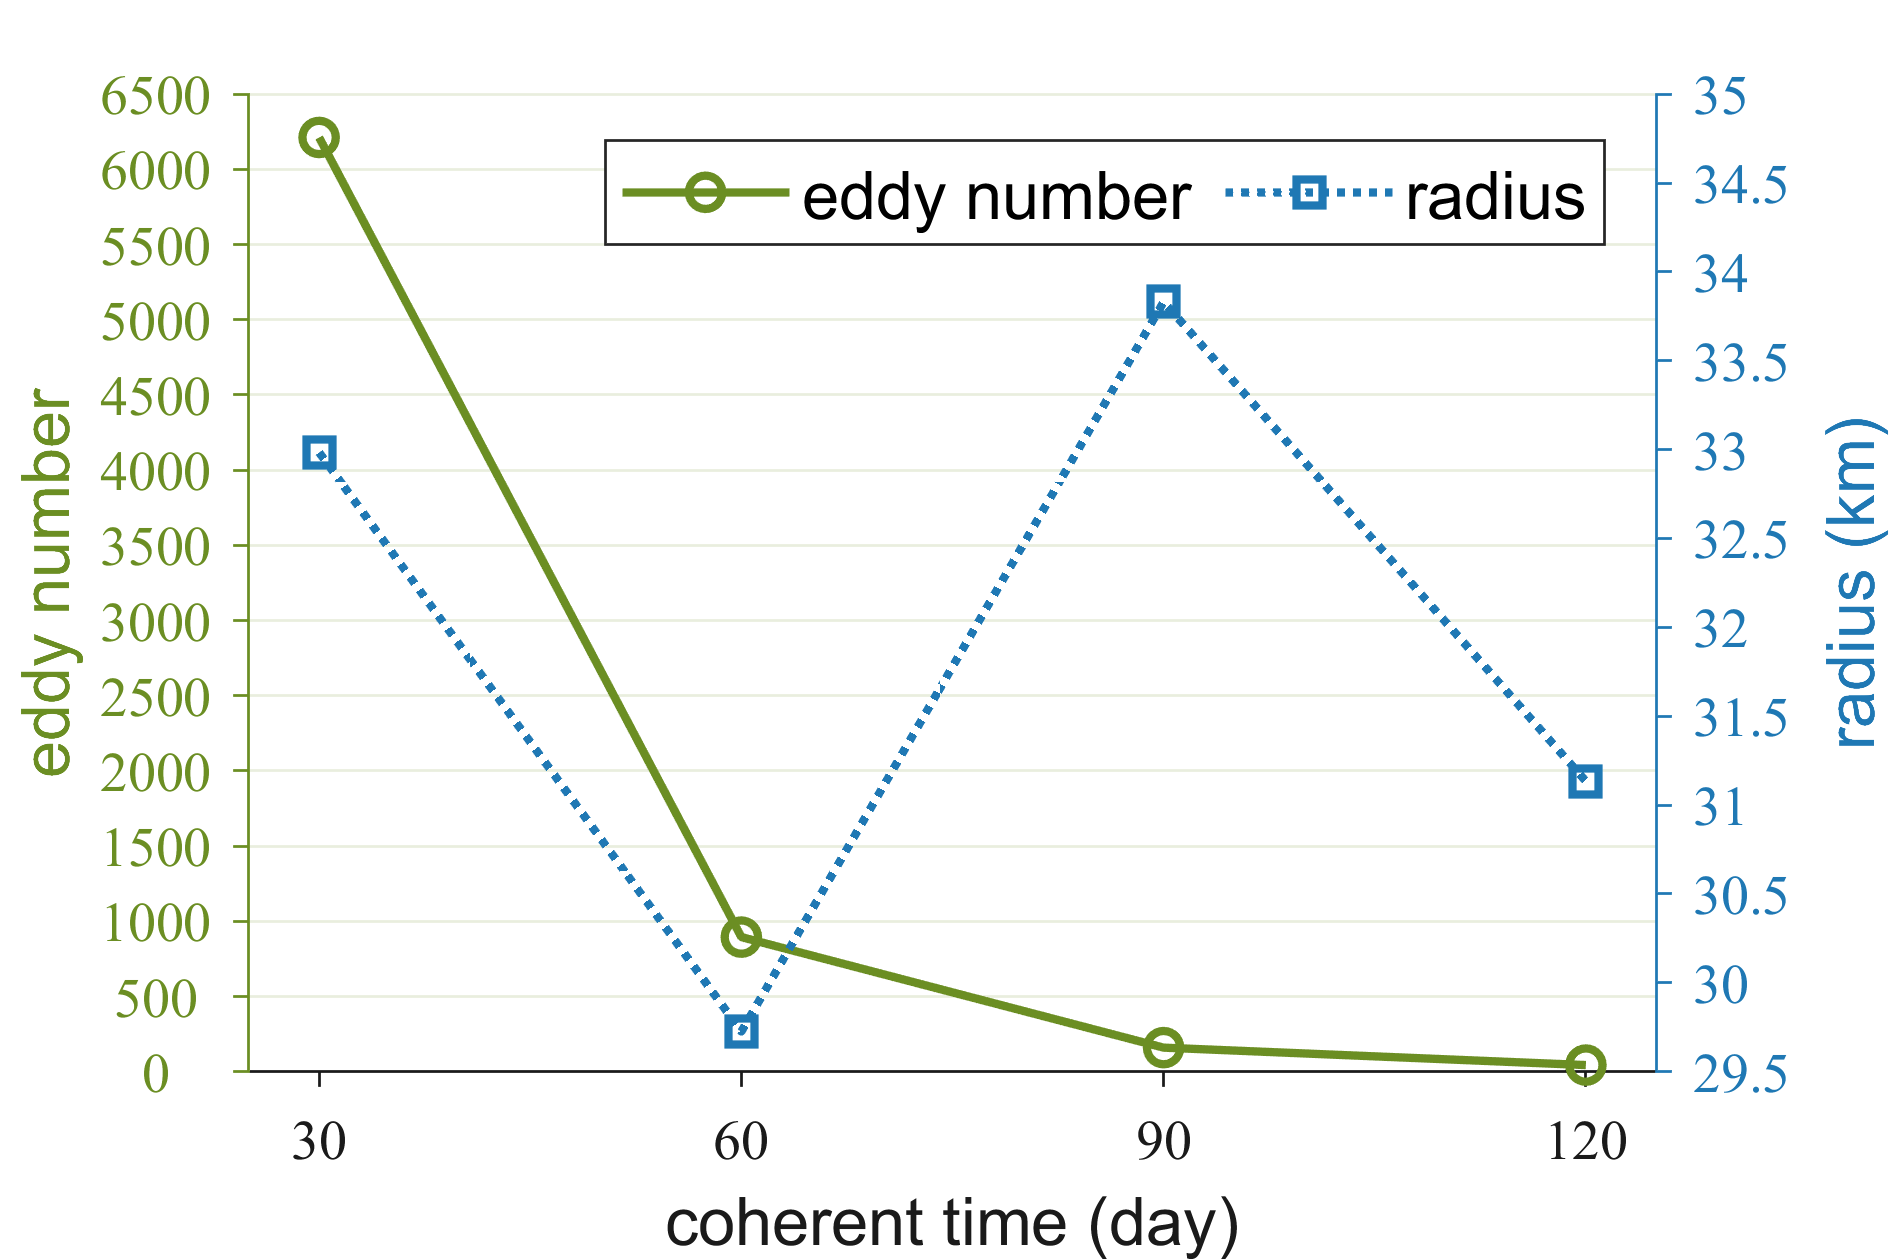
\includegraphics[width = 15cm]{chapter/figure/eddy coherent.png}
    \caption{Eddy properties and their relationship with coherence time}
    \label{eddy coherent}
\end{figure}

\begin{figure}[htbp]
    \centering
    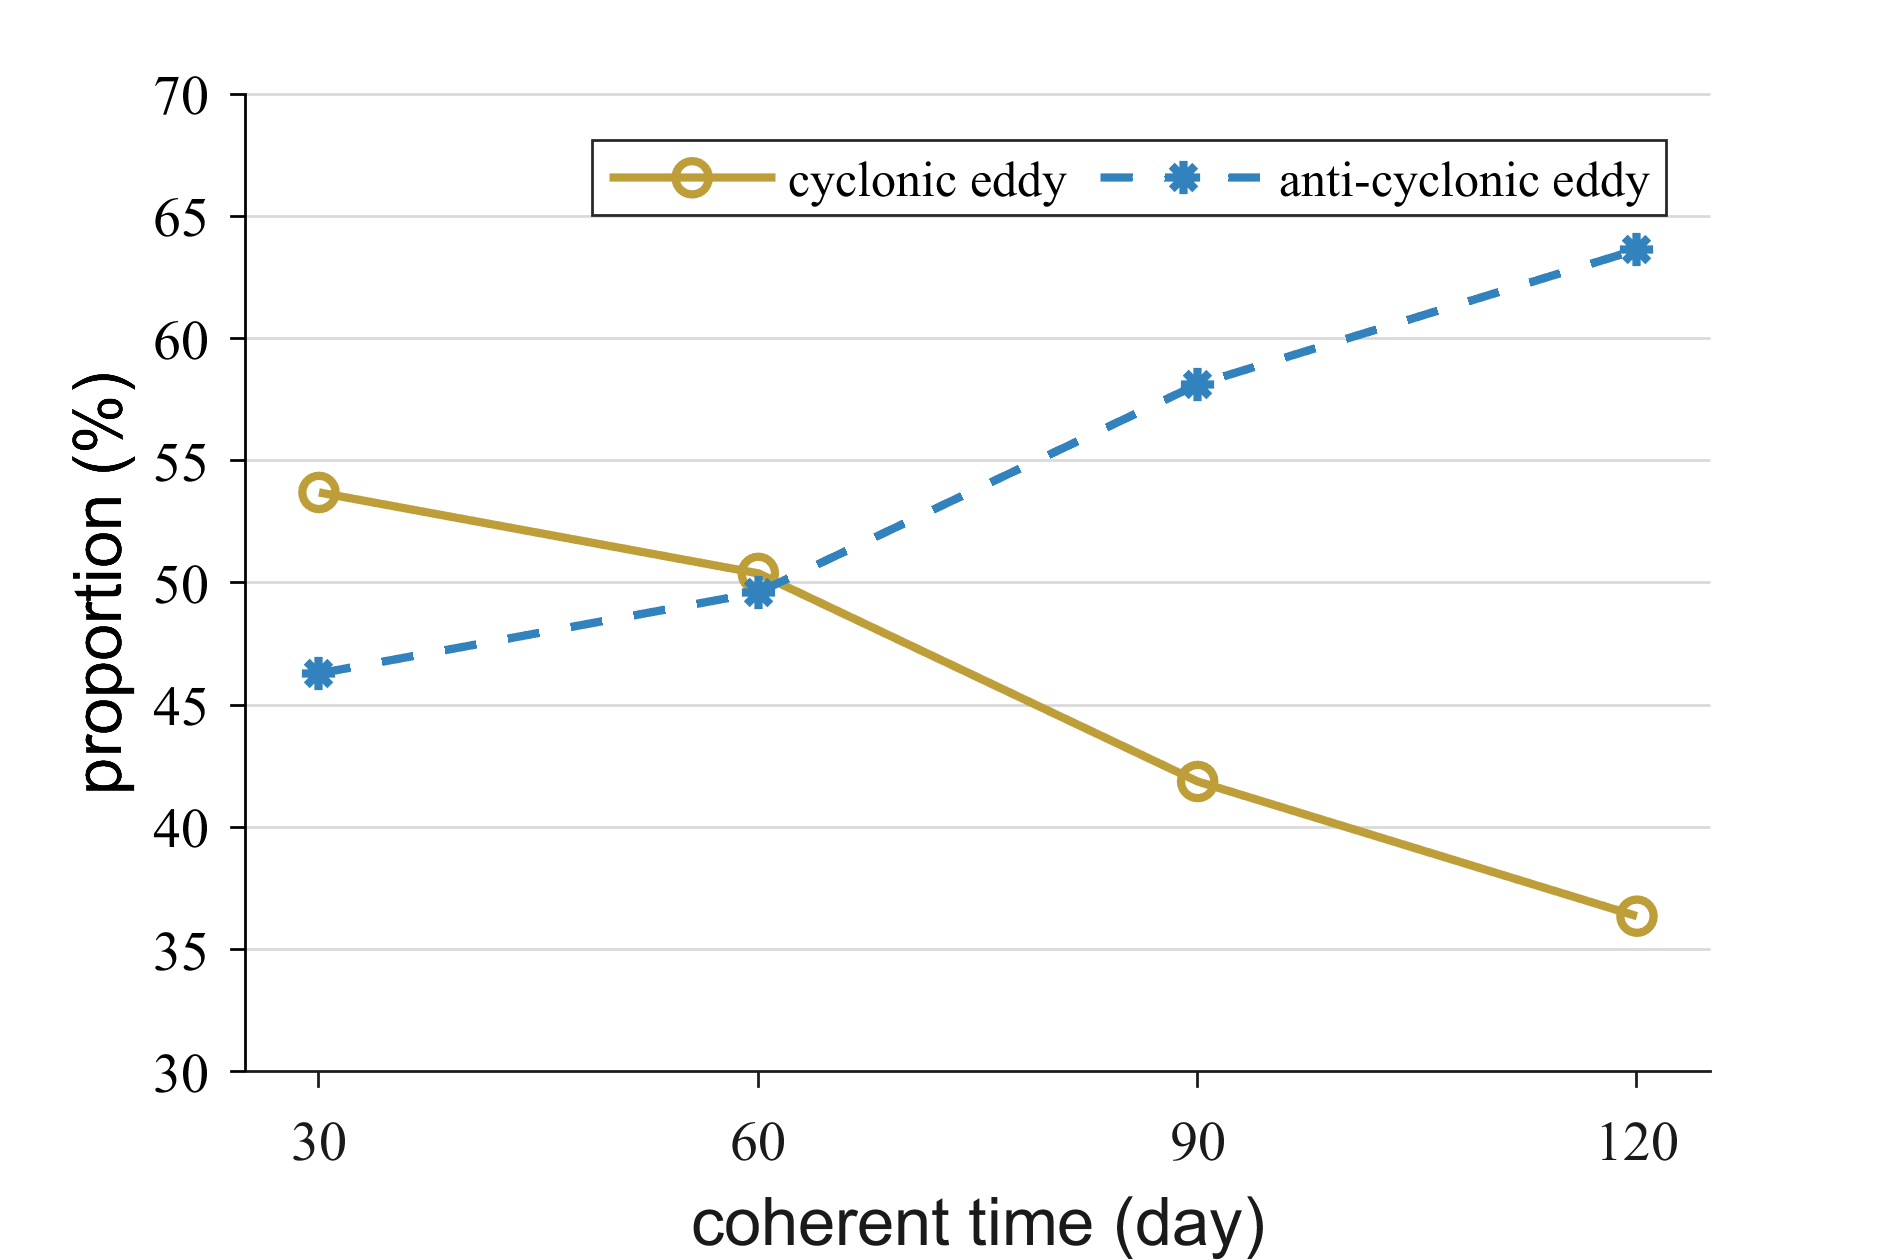
\includegraphics[width = 15cm]{chapter/figure/eddy type proportion.png}
    \caption{Eddy type proportion map}
    \label{eddy type proportion}
\end{figure}

Figure \ref{120-day eddies} shows three detected eddies with a coherent time of 120 days. In section (a) of the figure, the coherent time of the anti-cyclonic eddy originated in January 1998, the anti-cyclonic eddy shown in section (b) of the figure stemmed from September 2006 while the cyclonic eddy in section (c) was calculated using $t_0= September 2019$.In the figure, the initial position is marked with a black circle and the final position is marked in orange; anti-cyclonic eddy is indicated in red while cyclonic eddy is indicated in blue. They all show a westward propagation trend, carry water masses from the east to the west boundary, and finally the sea surface signal piles up at the west. 

\begin{figure}[htbp]
    \centering
    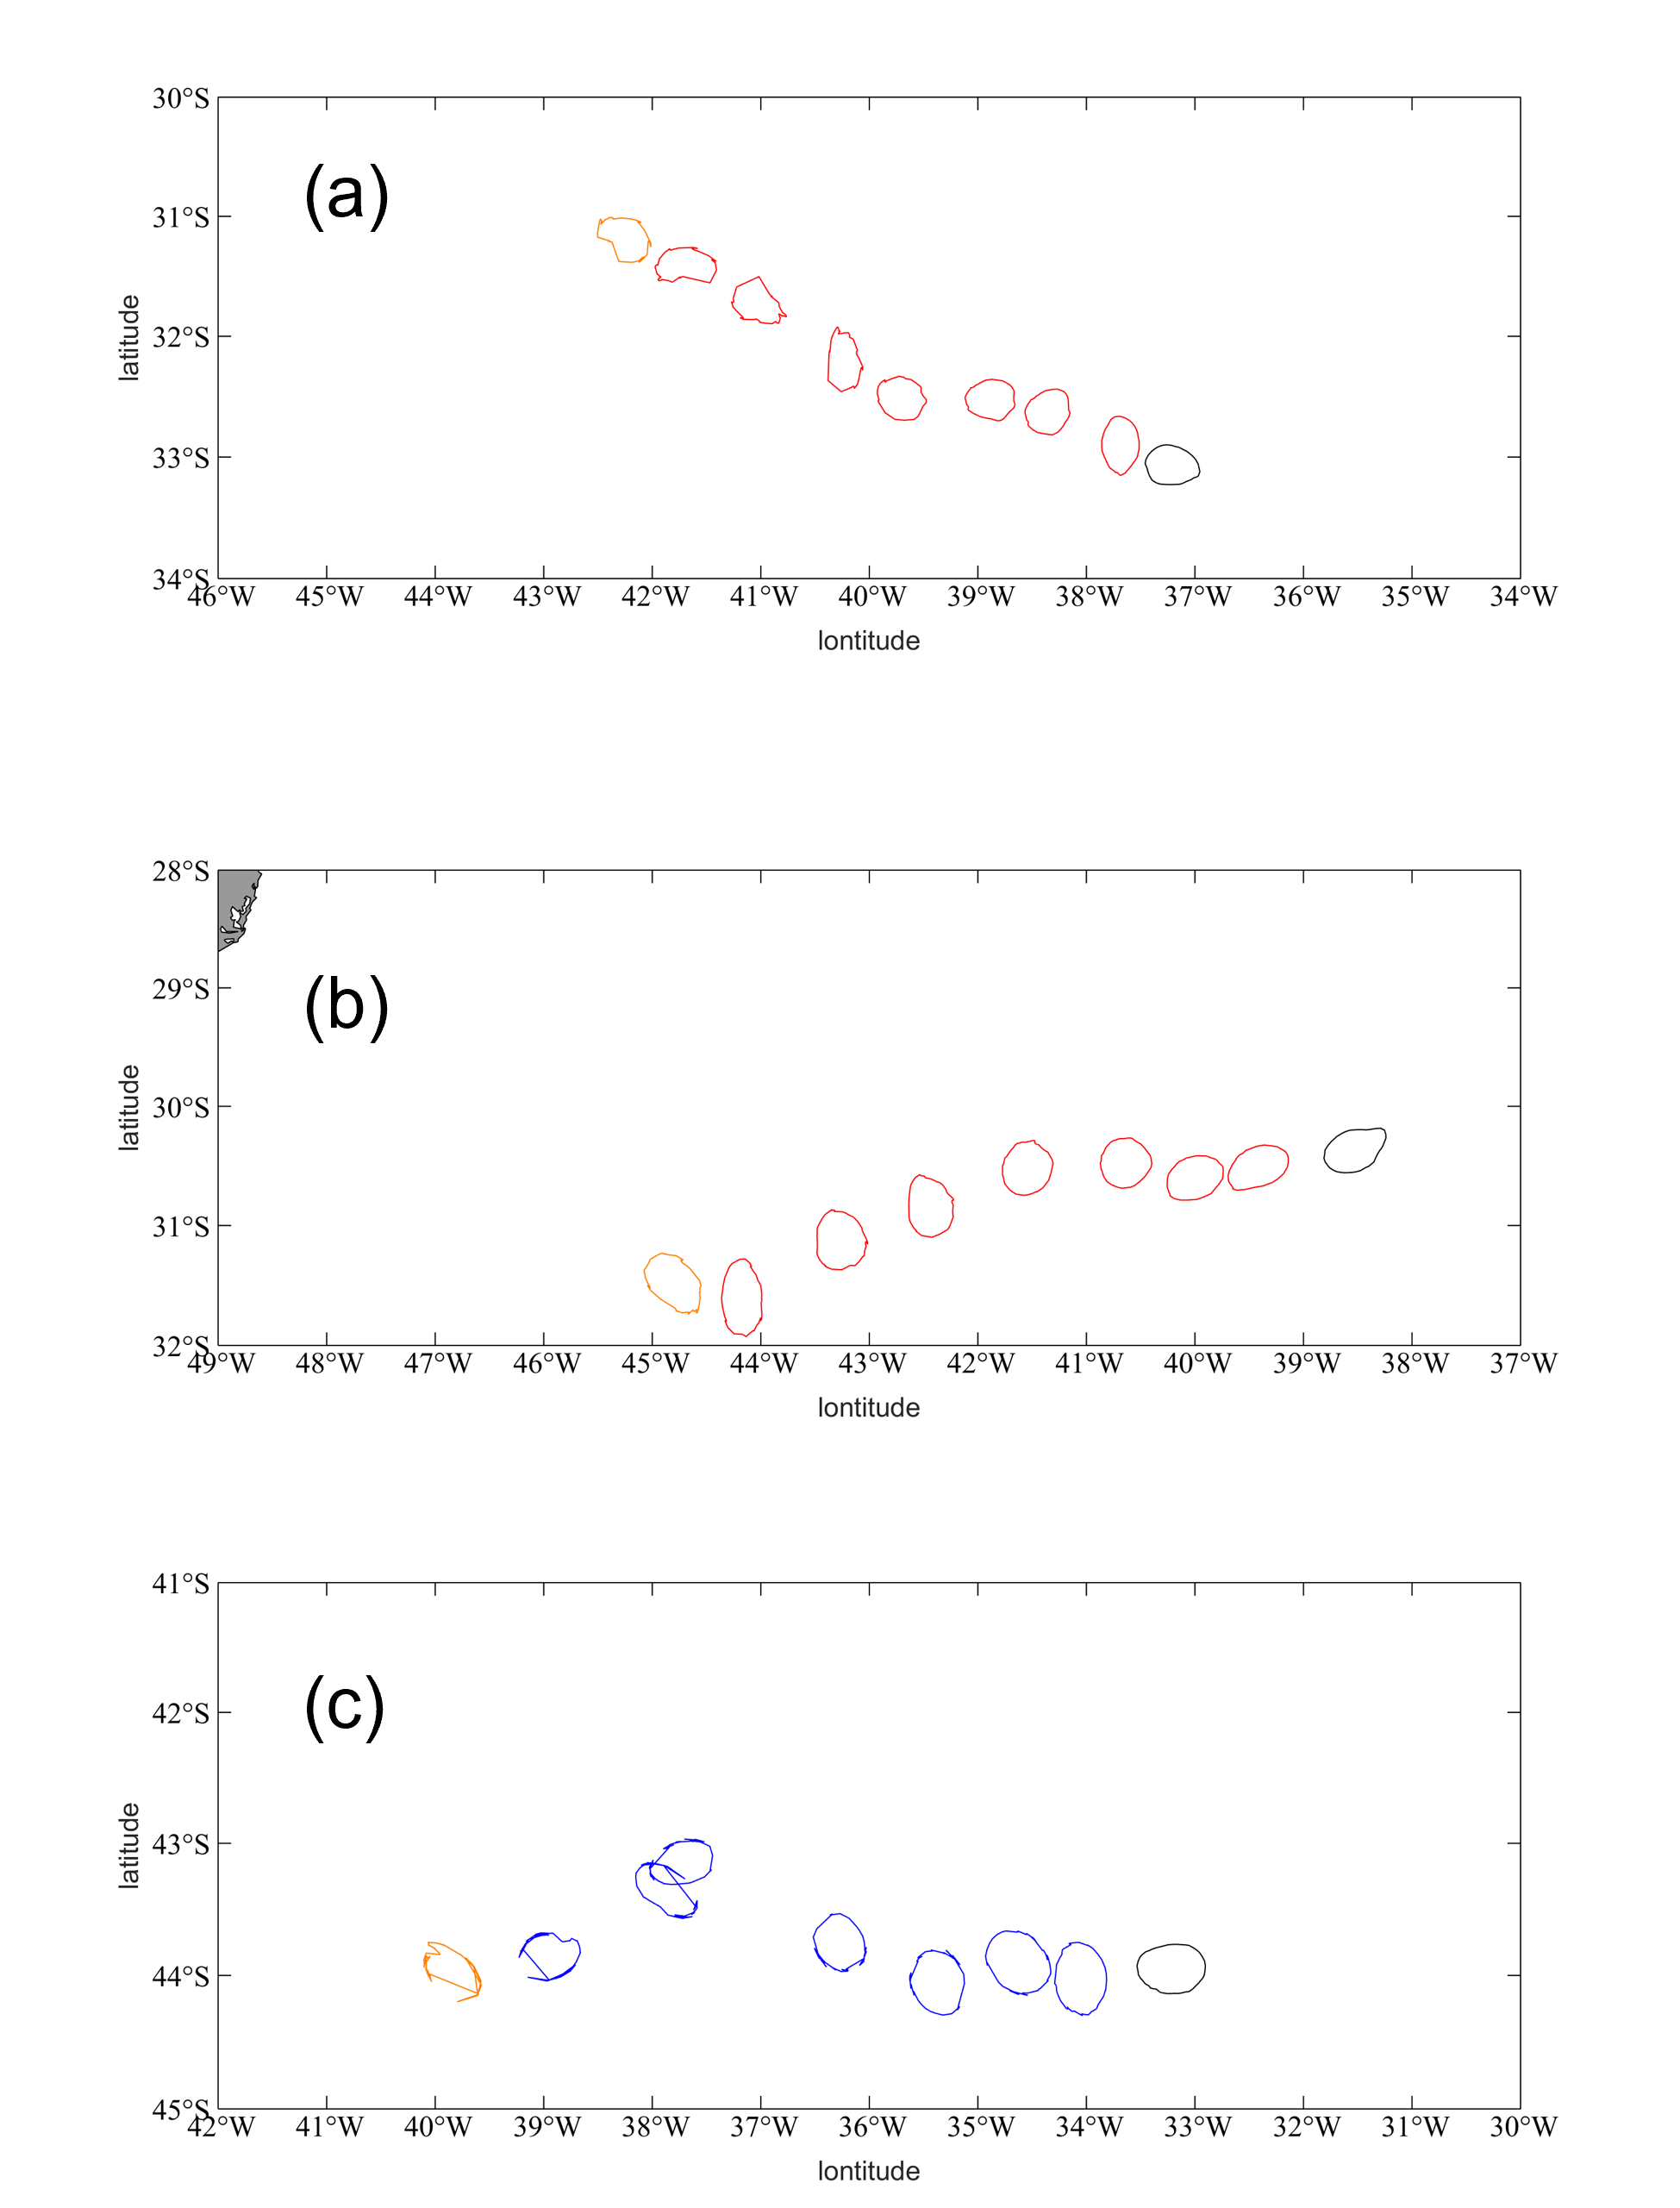
\includegraphics[width = 15cm]{chapter/figure/120-day eddies.png}
    \caption{Trajectories map of three 120-day vortices}
    \label{120-day eddies}
\end{figure}

\newpage

\section{Conclusion}

According to the criterion of the LAVD method, we have detected a total of 6212 coherent vortices, including 3336 cyclonic vortices and 2876 anticyclonic vortices from 1993 to 2019. There is an upward trend of eddies number. From the statistical results, there are obvious seasonal changes in the generation of anticyclonic vortices, which are more in spring and summer and less in autumn and winter.

Analysis of regional eddy statistics reveals hot spots of generation in the northeast part of the Argentine Basin and reveals the limitations of the LAVD method in high latitude regions and coastal shallow waters.

Lots of eddies have been observed in the southwest part of the Argentine Basin where Brazil Malvinas Confluence gives rise to baroclinic instabilities. The Center part of the Argentine Basin is associated with an eddy-free zone. The northern part of the Argentine Basin and connecting region between the Southern Ocean and the Argentine Basin are also the hot-spot of the oceanic eddy.

Eddies' radius decrease when the latitude is higher and the propagation speed is the largest in the middle latitude.

Vortex polarity has an effect on vortex properties: anticyclonic eddies are more stable and tend to have larger coherent time.






%\chapter{Three-dimensional eddies structures}\label{Three-dimensional eddies structures}

In this chapter, we present statistical and descriptive results of the vertical structures of oceanic eddies from 2013 to 2018 from the SOSE model dataset. Vortex penetration depth, radius distribution in each layer, and different patterns of cyclonic and anticyclonic eddies are discussed here.

\section{Introduction}

Although a lot of studies focusing on surface altimetry have investigated the horizontal properties of the oceanic eddies, very few of them can answer the questions of what the vertical profile of the eddies looks like and how they will affect the estimate of the volume transport. What is worst, some of the previous studies put forward prior assumptions about the vertical shape of the eddies and the mathematics-derived result may not be so robust. Some researchers want to deduce the vertical structure from Argo float data. However, time lag between the time when a float reaches the surface and the time when it reports its location with the Argos positioning satellite, and positioning errors limited by the accuracy of the Argos positioning system may raise the uncertainty of the identification\cite{chaigneau2011vertical}.

Most of the past research or publications only focus on the two-dimensional plot of oceanic eddies, partly because only the ocean surface observations are available, and partly because the magnitude of vertical velocity is three-orders less than the horizontal velocity, yielding a lot of noise to produce three-dimensional analysis and construct the three-dimensional structure. Sparse distribution of the observational array can only capture a limited picture of eddies features and thus ocean model, which provides a three-dimensional panoramic view of the ocean, fills in the gap in our understanding of three-dimensional ocean state variable 

One feasible solution is using Lagrangian tools such as drifts or Argo floats, with the hope that drifts are located around the eddy cores and the selected interpolation scheme is suitable to estimate the real oceanic state around the eddies.

Questions still exist about the three-dimensional structure of oceanic eddies: (1) how do the eddies extend in the vertical direction; (2) how do eddies enhance the stirring and coupling of the upper ocean and deep ocean.

There is great concern about the understanding gap between the surface eddies and deep eddies. The ocean is divided into three zones in the vertical direction: a well-mixed surface region, rapidly varying ocean subsurface thermocline, and the stratified ocean interior. The ocean surface and ocean interior, with distinct features and separated by the thermocline, set up the questions about the relationship between surface eddies and deep eddies. Some eddies are constrained only to the surface, some will extend to the deep sea, while others subsurface eddies show no sign of the surface height signal. Worse still, it is rather difficult to extract Lagrangian
structures and elaborate their effect on mixing properties in unsteady 3-D flow due to the explosion of complexity \cite{aref2017frontiers}.  

\section{3D structure construction algorithms for an eddy}

In chapter \ref{Lagrangian eddies detection}, we show how to set up a computational process and detect eddy on the surface. Repeating the same process and using the flow field information at 42 layers in the numerical data, we could get the 3D structure of coherent eddy. As discussed in the previous paper, an eddy center would not drift by 1/4
of its radius when it goes down 50 m if it is still detectable \cite{dong2012three}.

Thus, the overall workflow of the detection would be as follows:

\begin{itemize}
  \item [1)] 
  Compute the LAVD field in each depth layer and extract eddies from the surface layer to the other below layers following the same process in Chapter \ref{data and methodology}.
  \item [2)]
  Group the extracted eddies according to their characteristics and then  select eddies based on judging criteria ``an eddy center would not drift by 1/4 of its radius when it goes down 50 m".
  \item [3)]
  If in the same depth level, more than one eddies were found, pick the vortex with the closest horizontal distance from the surface one.
\end{itemize}


\section{Eddies penetration depth and three-dimensional shape type}

To construct the vertical profile of the eddies, we use the velocity filed results generated from SOSE oceanic model. The horizontal resolution of SOSE dataset is $ \frac{1}{6}^{\circ} $ and SOSE dataset has 41 layers in the vertical direction in total, covering variables from the surface to 5km in depth.

We have detected 732 eddies in the surface layer from 2013 to 2018 and 566 ($77\%$) of them were found to have signals in the below layers and  used to construct the 3-D structure in the research, which suggests an amount of about $25\%$ of the eddies is quite shallow

From figure \ref{Depth Frequency.png}, we could find that about half of the eddies could still be detected at a depth of 2010 meters, about $20\%$ of the eddies have depths ranging from 1500 m to 1800 m, and about $18\%$ of them reach the depth of 1000m to 1500 m.

\begin{figure}[htbp]
    \centering
    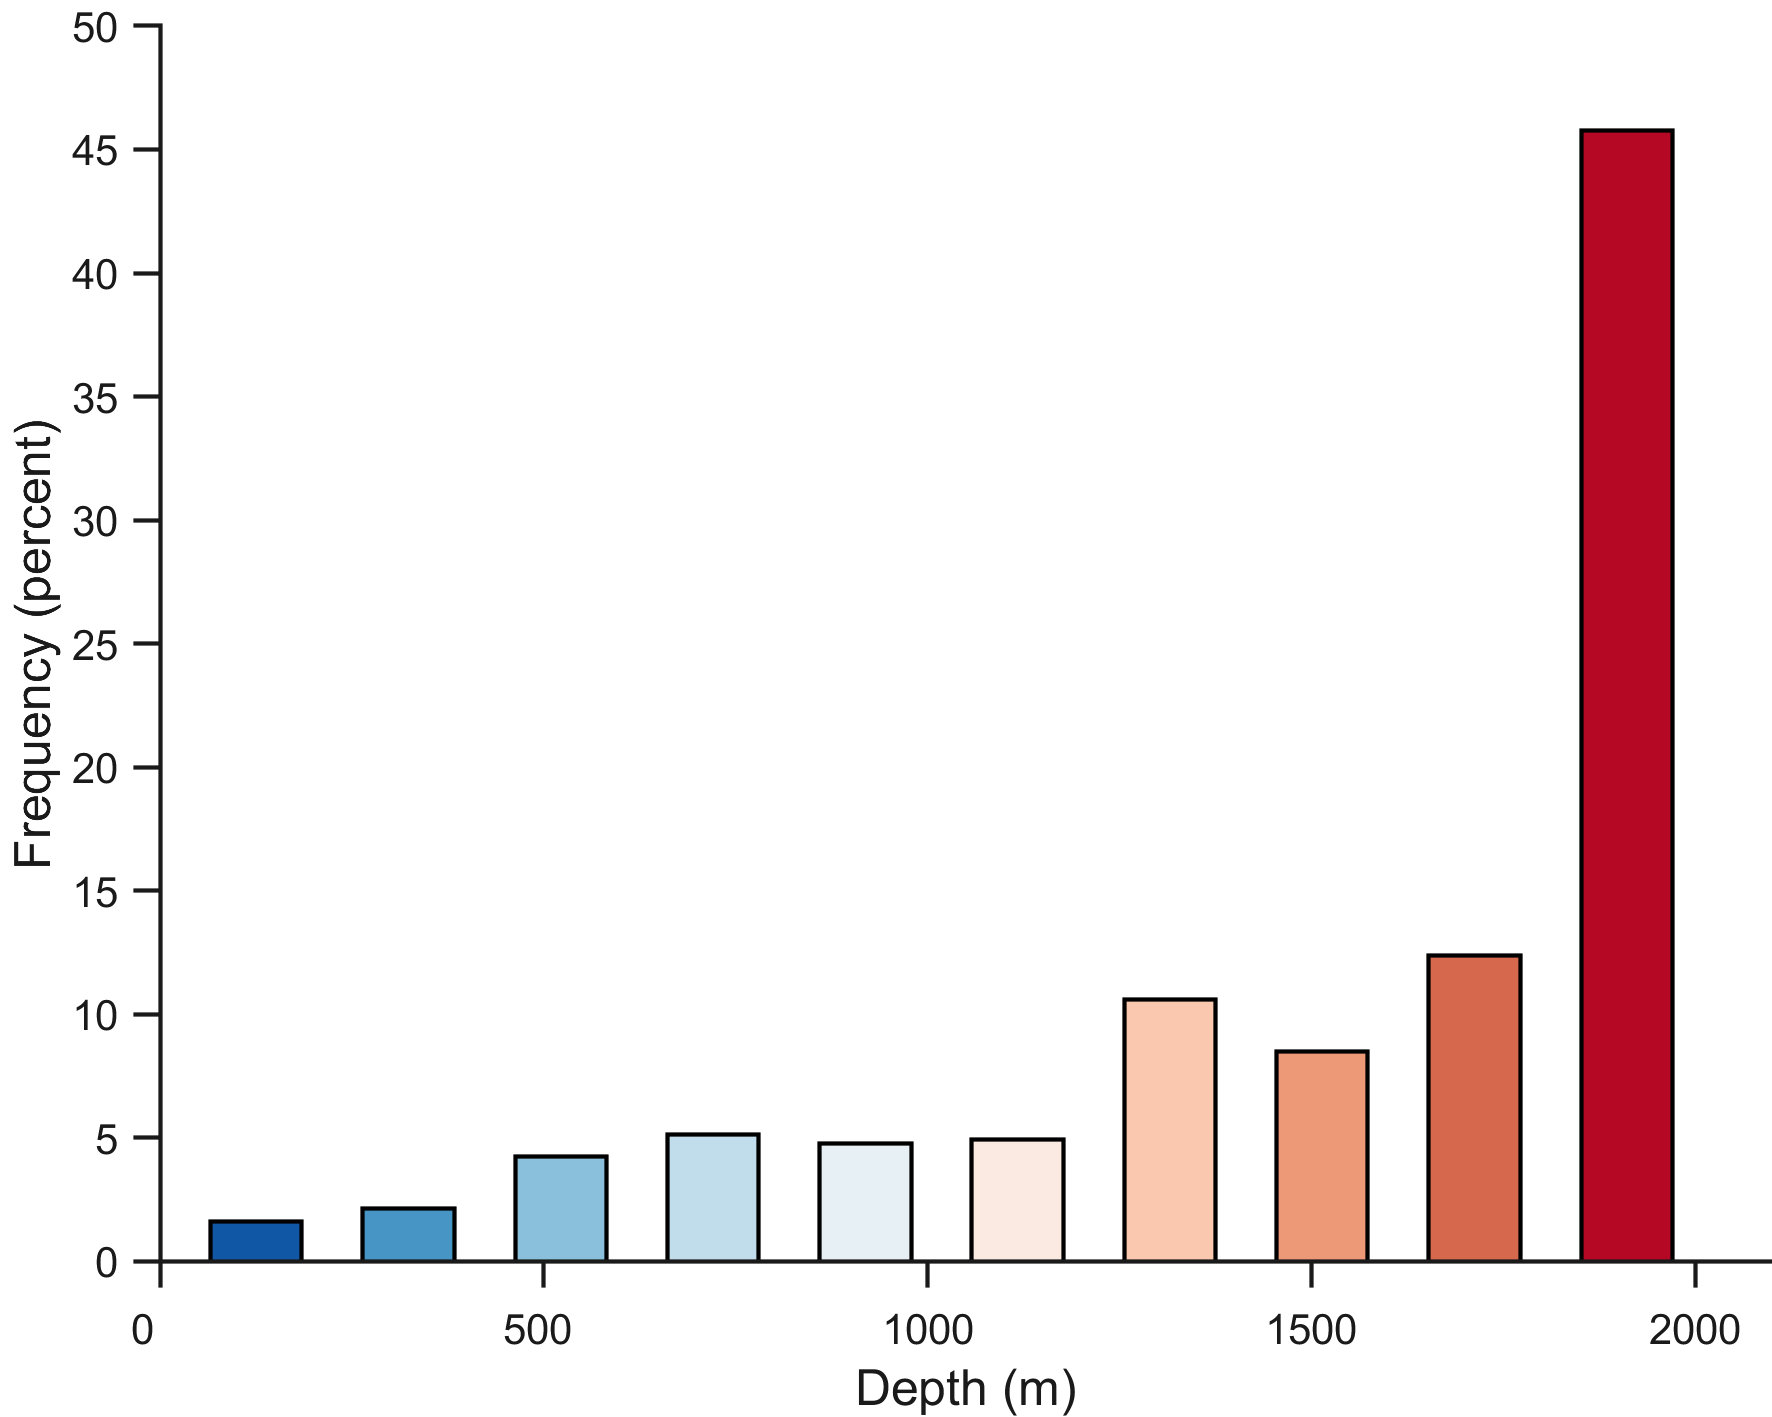
\includegraphics[width =12cm]{chapter/figure/Depth Frequency.png}
    \caption{Histogram distribution map of vortex depth}
    \label{Depth Frequency.png}
\end{figure}

Among all the 566 3-D eddies, about $52\%$ of them (294) are cyclonic eddies and about $48\%$ of them are anticyclonic ones. The maximum vortex radius of the cyclonic eddies is placed at depth of around 826 meters while the maximum vortex radius of the anticyclonic eddies centers at depth of 659 meters or so. The average value of the maximum depth of the cyclonic vortices is about 1679 meters and the mean value of the maximum depth of the depth extension of anticyclonic eddies is 1496 meters. The above findings show us that cyclonic eddies tend to have a greater vertical extension and thus they have stronger transport capacity and could carry more volume of seawater.

According to existing papers, the eddy vertical shape of oceanic eddies could be classified into three kinds: eddies with the largest semidiameter on the surface like a bowl, cone-shaped vortices with the largest radius at the bottom layer, and lens-shaped eddies having the largest size in the middle \cite{dong2012three,lin2015three}.

In the Argentine basin, all those three types of eddies were found and lens-shaped eddies are the majority:  72 of the detected eddies were bowl-shaped, 412 of them are lens-shaped and 82 of the eddies are cone-shaped vortices. The following figures from \ref{bowl-shaped.png} to \ref{cone-shaped.png} show the vertical distribution of some selected eddies. Figure \ref{bowl-shaped.png} illustrates three bowl-shaped eddies having a maximum radius on the surface and then decreasing towards the bottom. Figure \ref{lens-shaped.png} shows three eddies having maximum radius in the intermediate layer and then becoming smaller with increasing depth. In figure \ref{cone-shaped.png}, eddies on the surface are the smallest, gradually get larger, and reach a maximum at the bottom. The vortex radius may be more stable in size in the intermediate layer.

\begin{figure}[htbp]
    \centering
    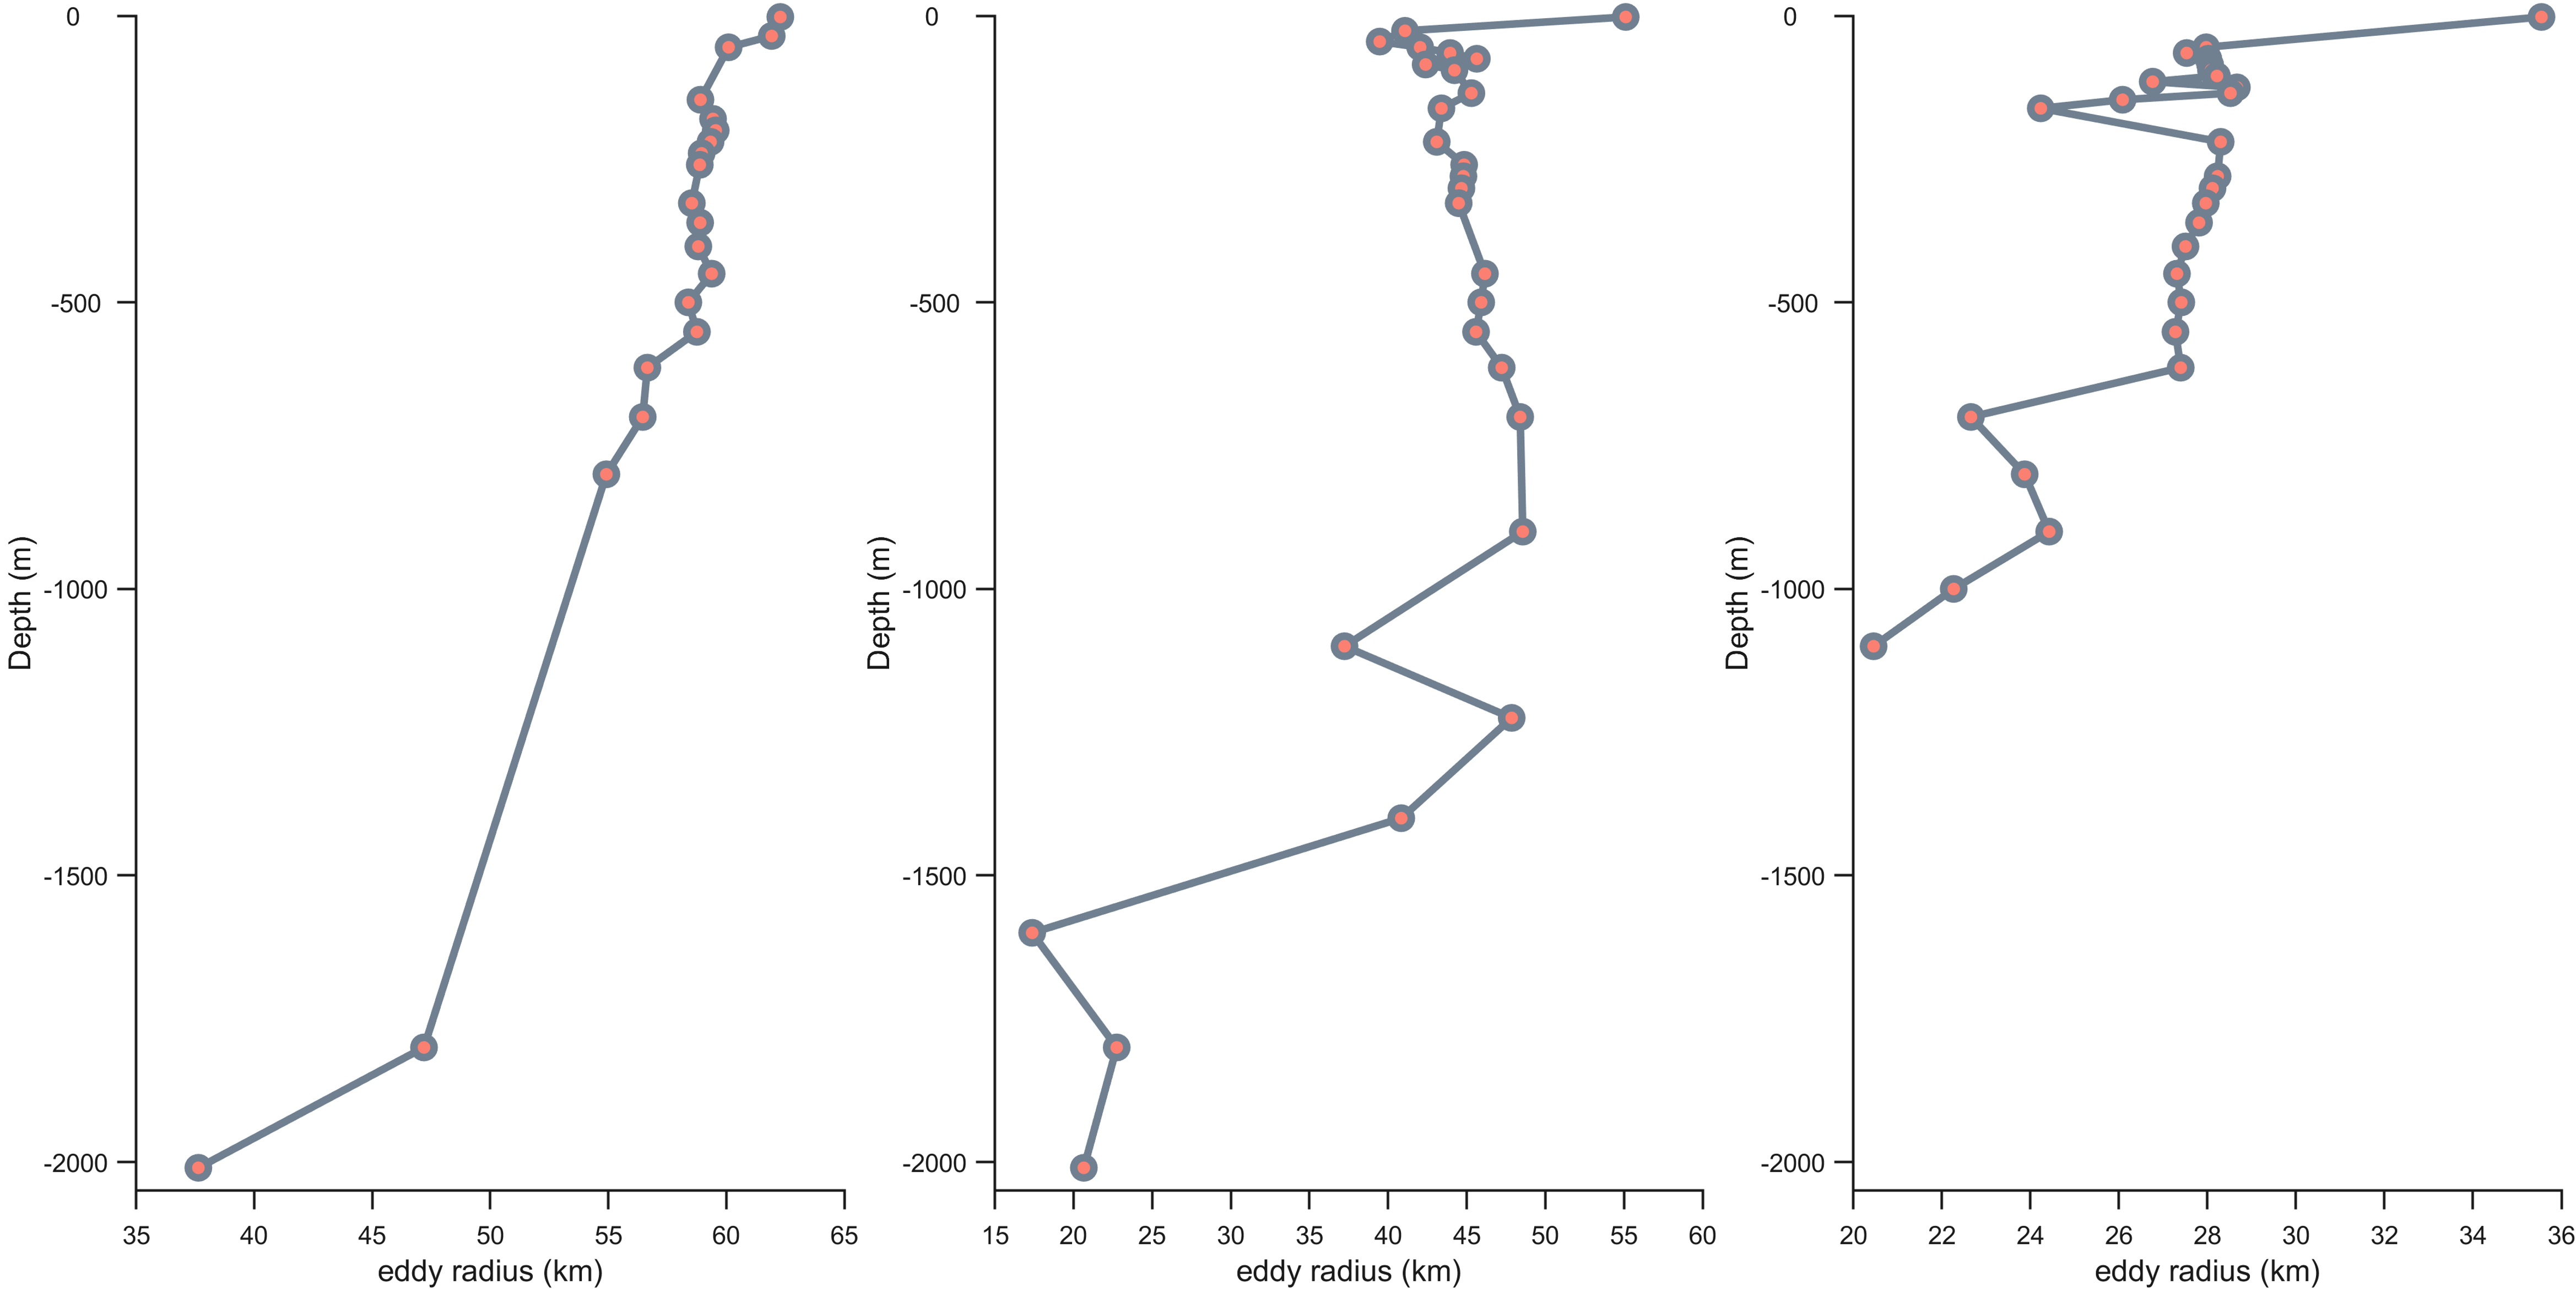
\includegraphics[width=1.0\textwidth]{chapter/figure/bowl-shaped.png}
    \caption{Three examples of bowl-shaped eddies}
    \label{bowl-shaped.png}
\end{figure}

\begin{figure}[htbp]
    \centering
    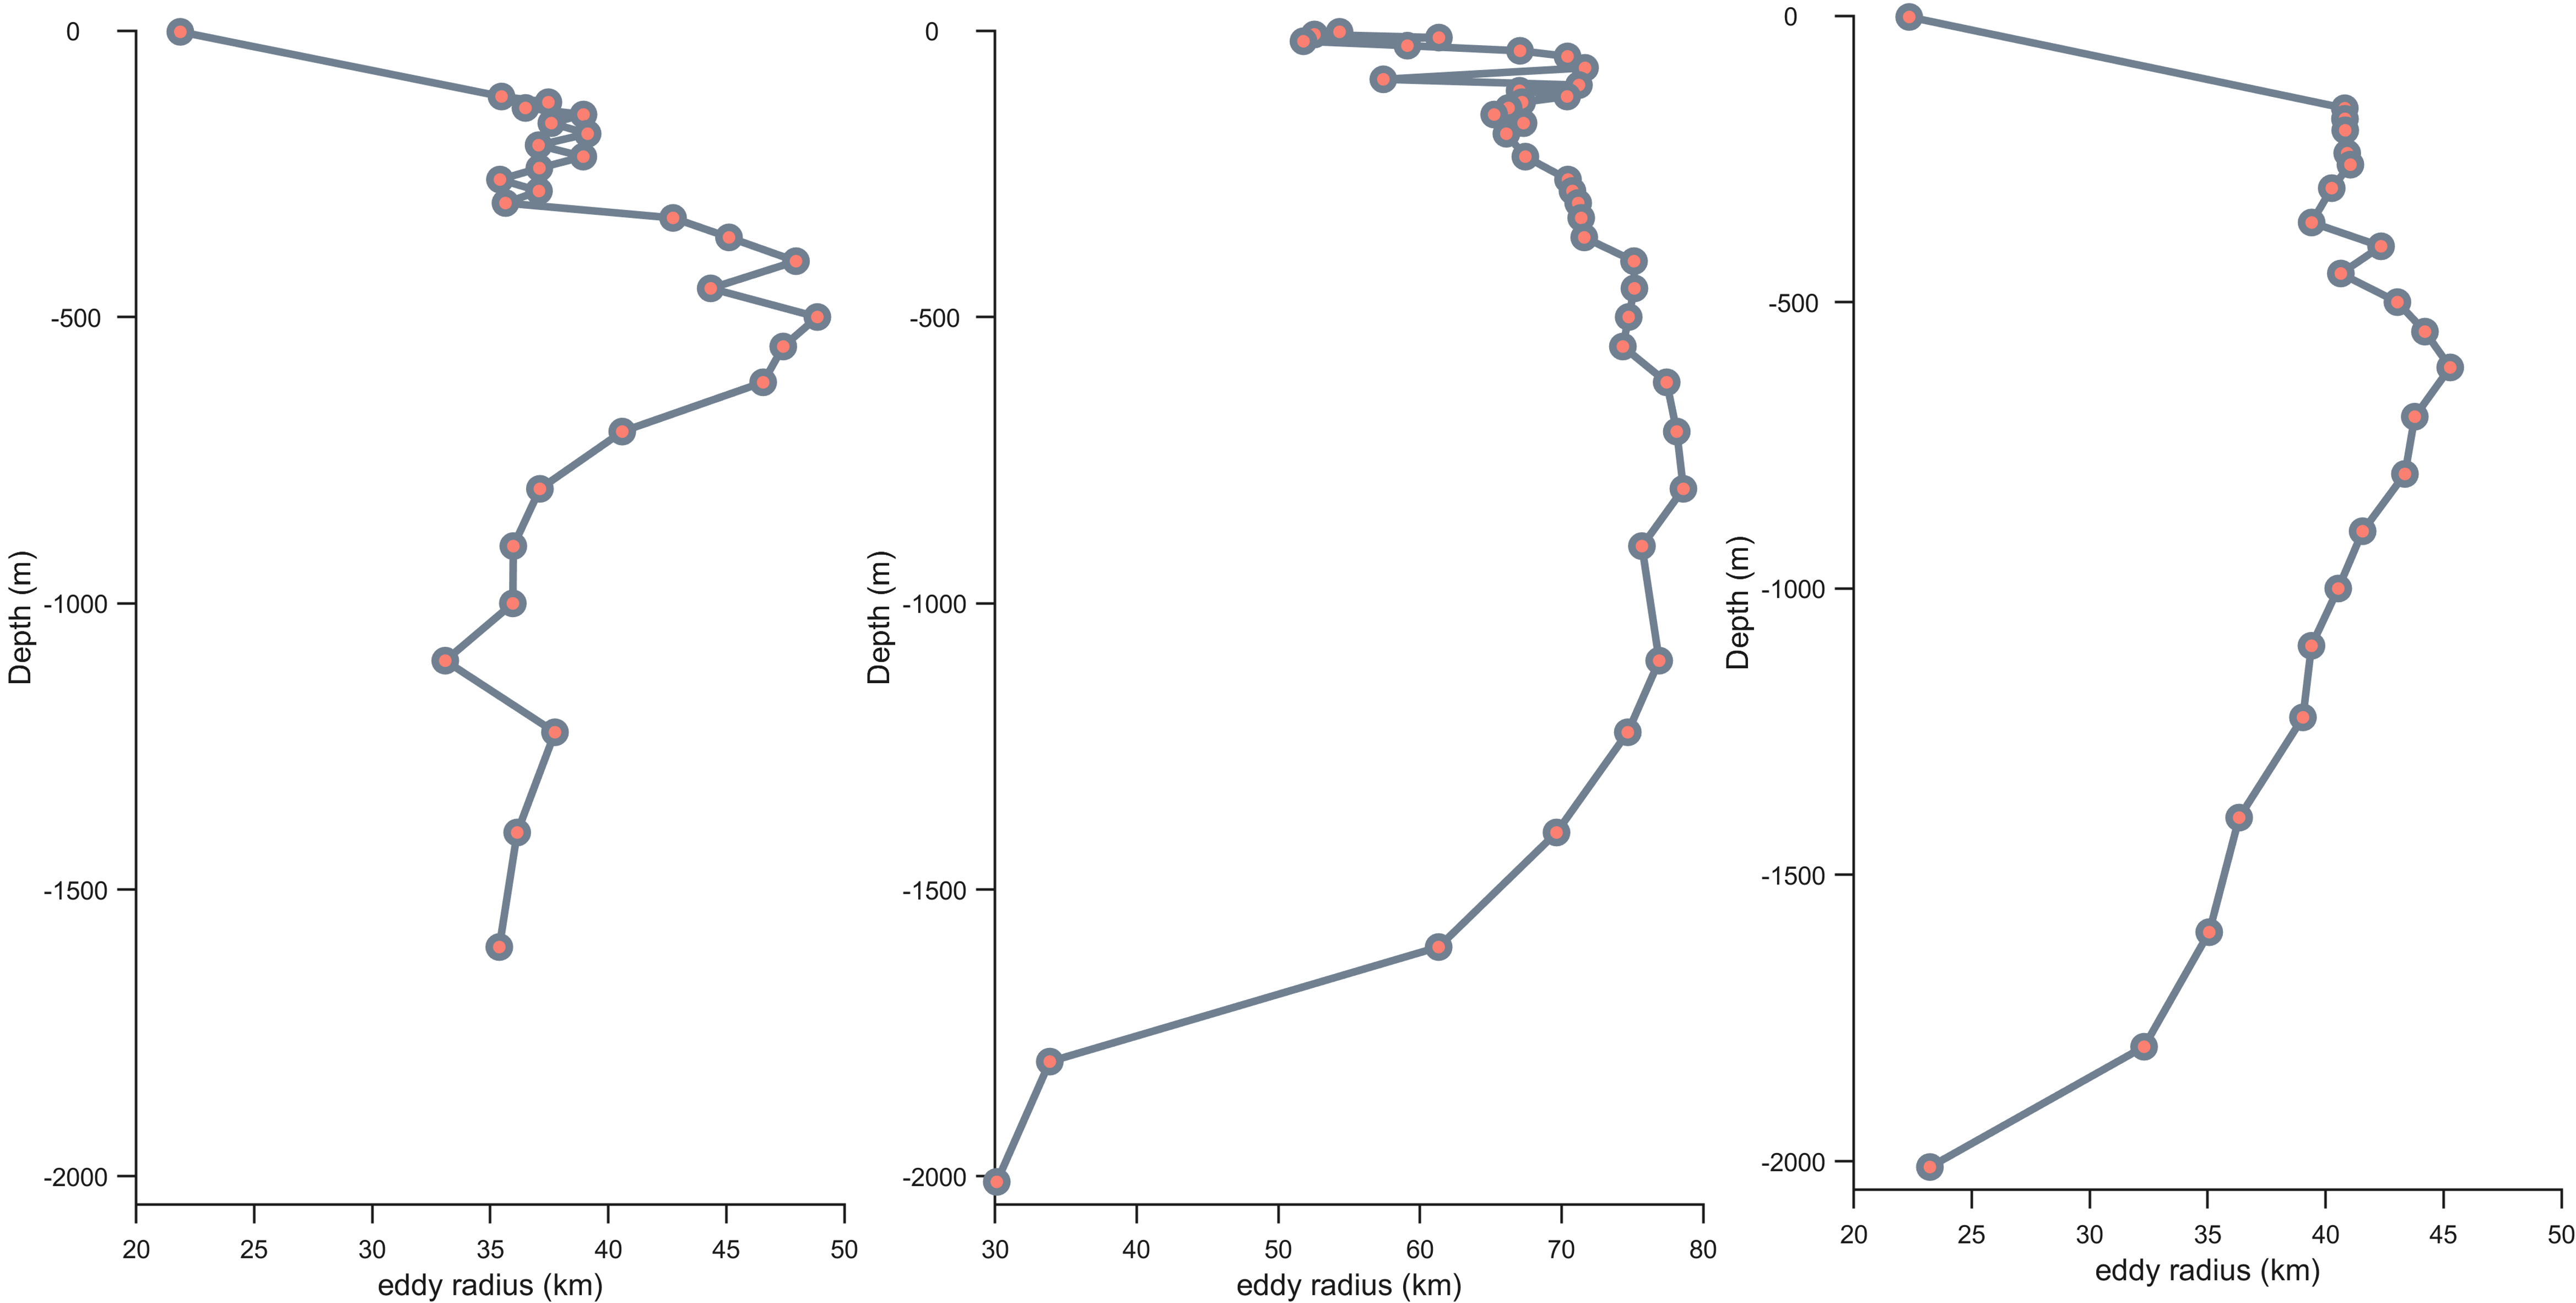
\includegraphics[width = 15cm]{chapter/figure/lens-shaped.png}
    \caption{Three examples of lens-shaped eddies }
    \label{lens-shaped.png}
\end{figure}

\begin{figure}[htbp]
    \centering
    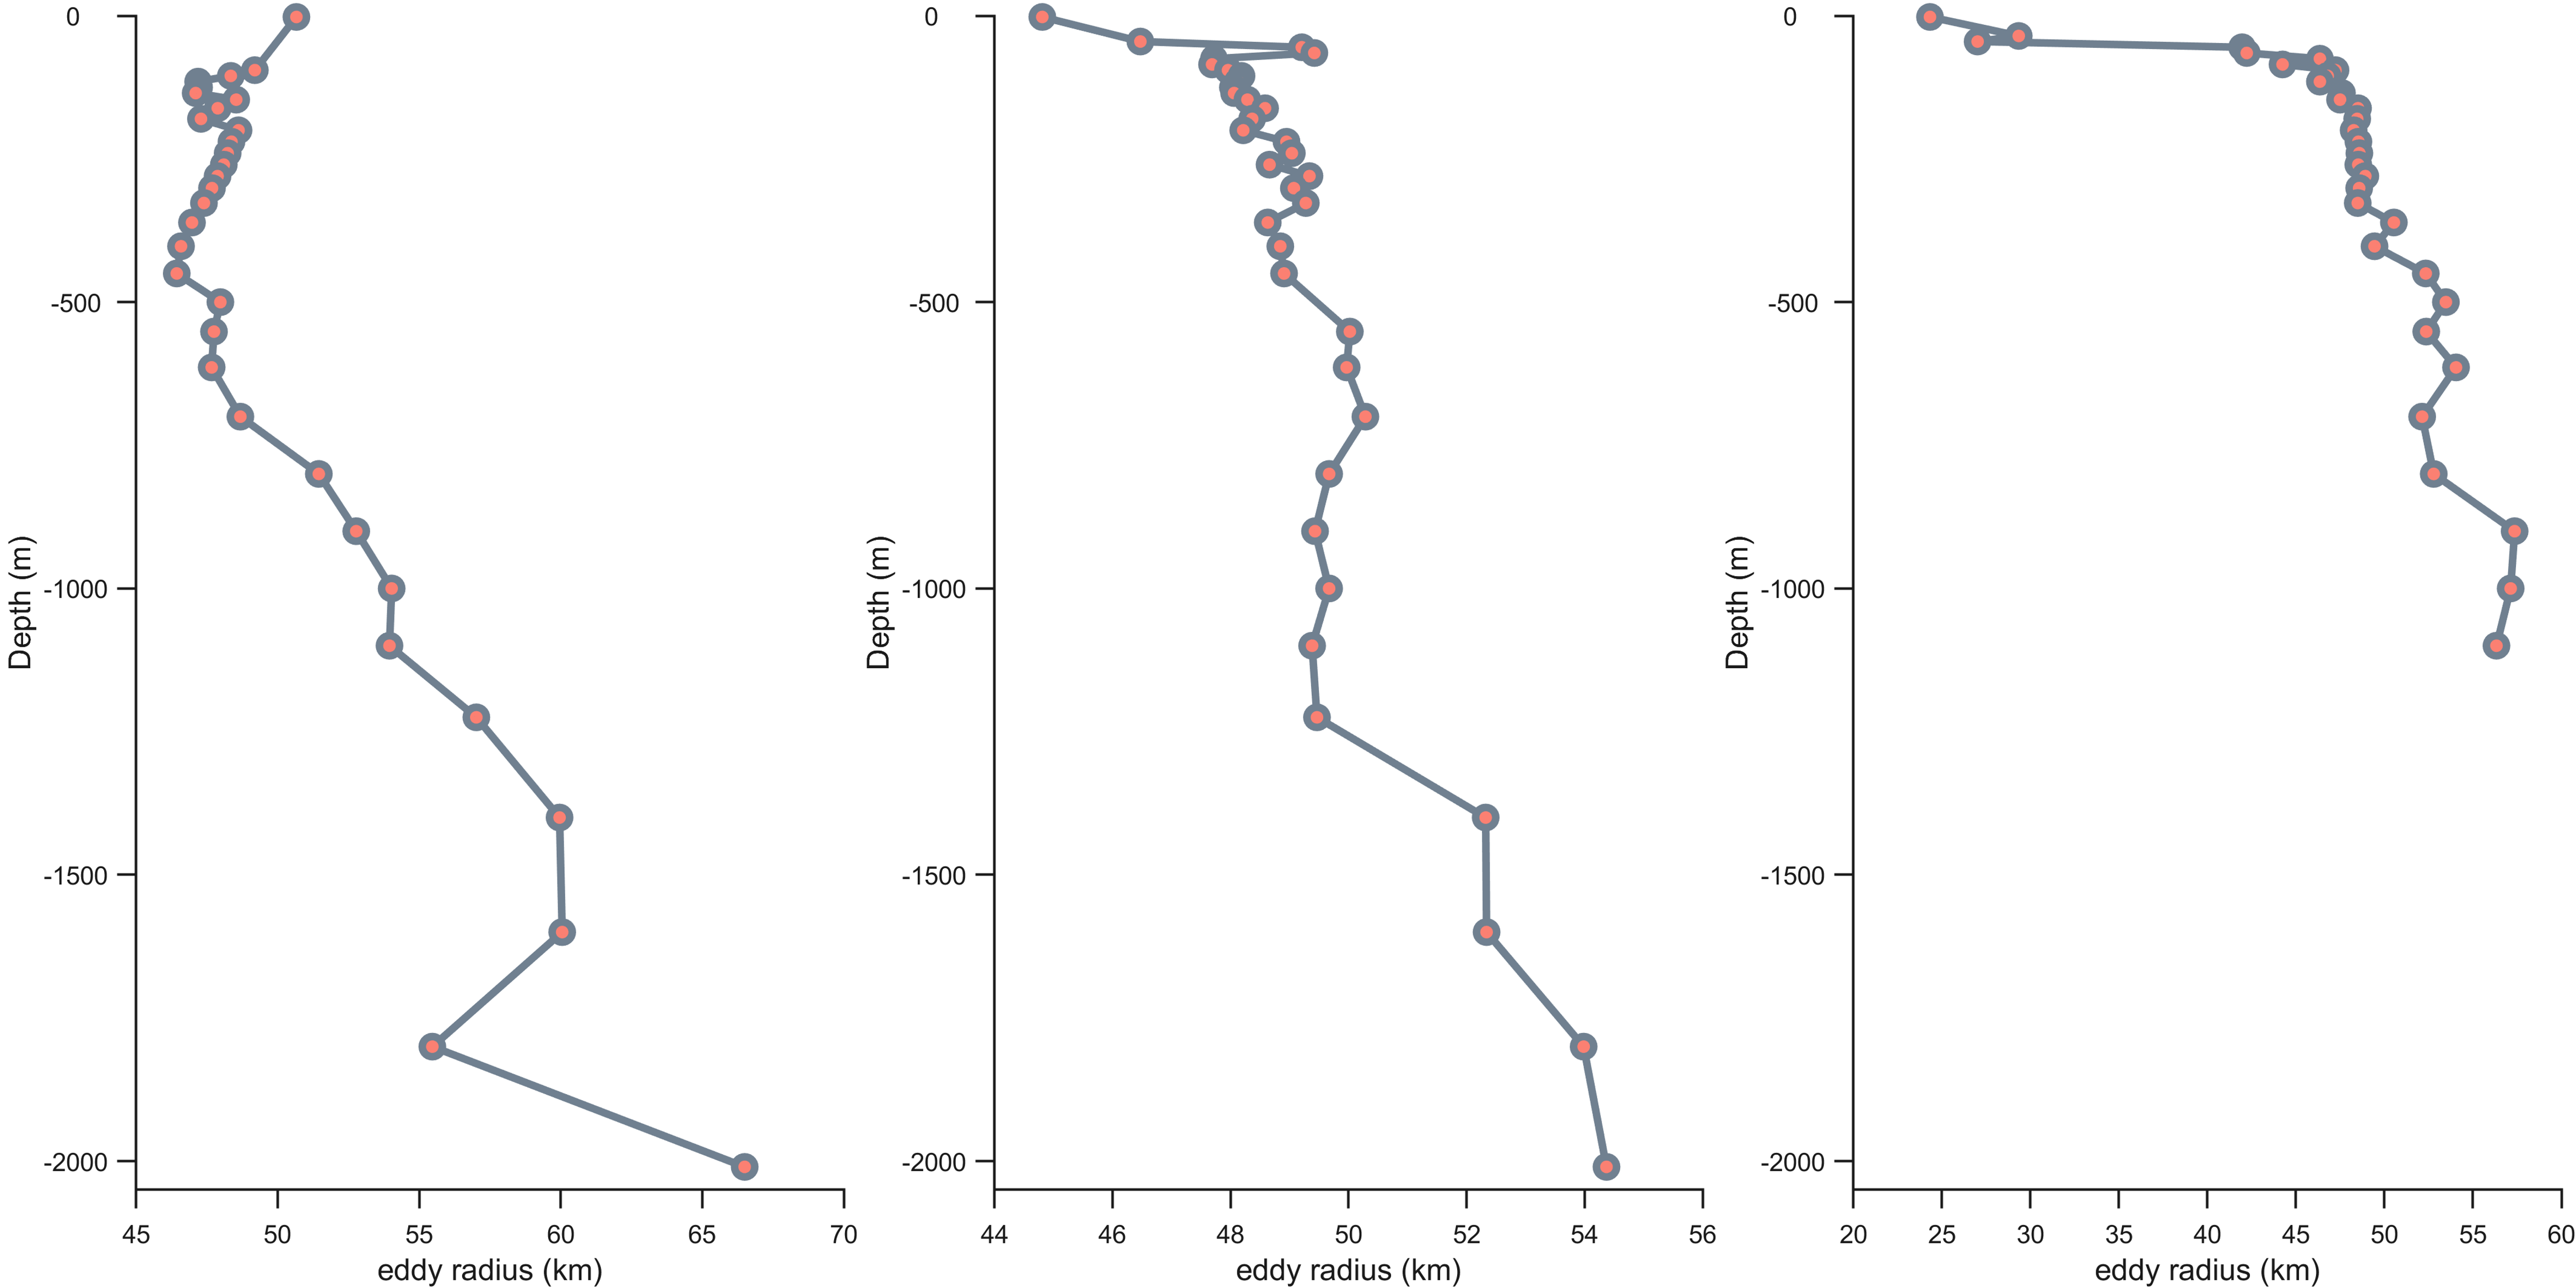
\includegraphics[width = 15cm]{chapter/figure/cone-shaped.png}
    \caption{Three examples of cone-shaped eddies}
    \label{cone-shaped.png}
\end{figure}





\section{Case studies of oceanic eddies}

Figure \ref{cyclonic-3D.png} shows the vertical slice of salinity field and radius distribution of a cyclonic coherent eddy with $t_0 = 2014-01-01$. We could find that the subsurface vortex radius has a maximum value of and the eddy's size changes dramatically on the surface. In section (a) of the figure \ref{cyclonic-3D.png}, each slice represents the salinity distribution in each depth layer. The minimum value of the salinity is at the blue end of the color chart while the maximum value of the regional salinity is represented by the red color of the color chart; the color bar shown on the left side  only displays the salinity limit on the bottom layer. The surface eddy is the center of the negative anomalous envelope of salinity and in the below layers, the eddy is surrounded by high salinity contour. These findings suggest that cold and salty coherent cyclonic eddy may upwell the bottom water column into the subsurface layers. 

Figure \ref{2014-12-24_6.png} shows an anticyclonic eddy with maximum radius in the intermediate layer and $t_0 = 2014-12-01$. It has a warm core of the water in the center of the eddy. However, the area of the high-temperature contour is much bigger than the area enclosed by the eddy, which we could infer that coherent water transport capabilities carried by the coherent eddy may be much weaker than what we have expected in an Eulerian instantaneous field.  

However, in some of the cases, the extreme value of the background salinity ($S$) or temperature ($\theta$) field does not match the core of the coherent eddies. In some of the cases, the background extrema of $S$ or $\theta$ may shift a little bit from the eddy center. This asymmetry feature is more obvious in the vertical structure of anticyclonic eddies \cite{sandalyuk2021three}.

What is more, the above rules are not so robust in the surface layer, especially the first 100 meters, which suggests the other boundary layer mixing processes can significantly affect the character of the vortex.


\begin{figure}[htbp]
    \centering
    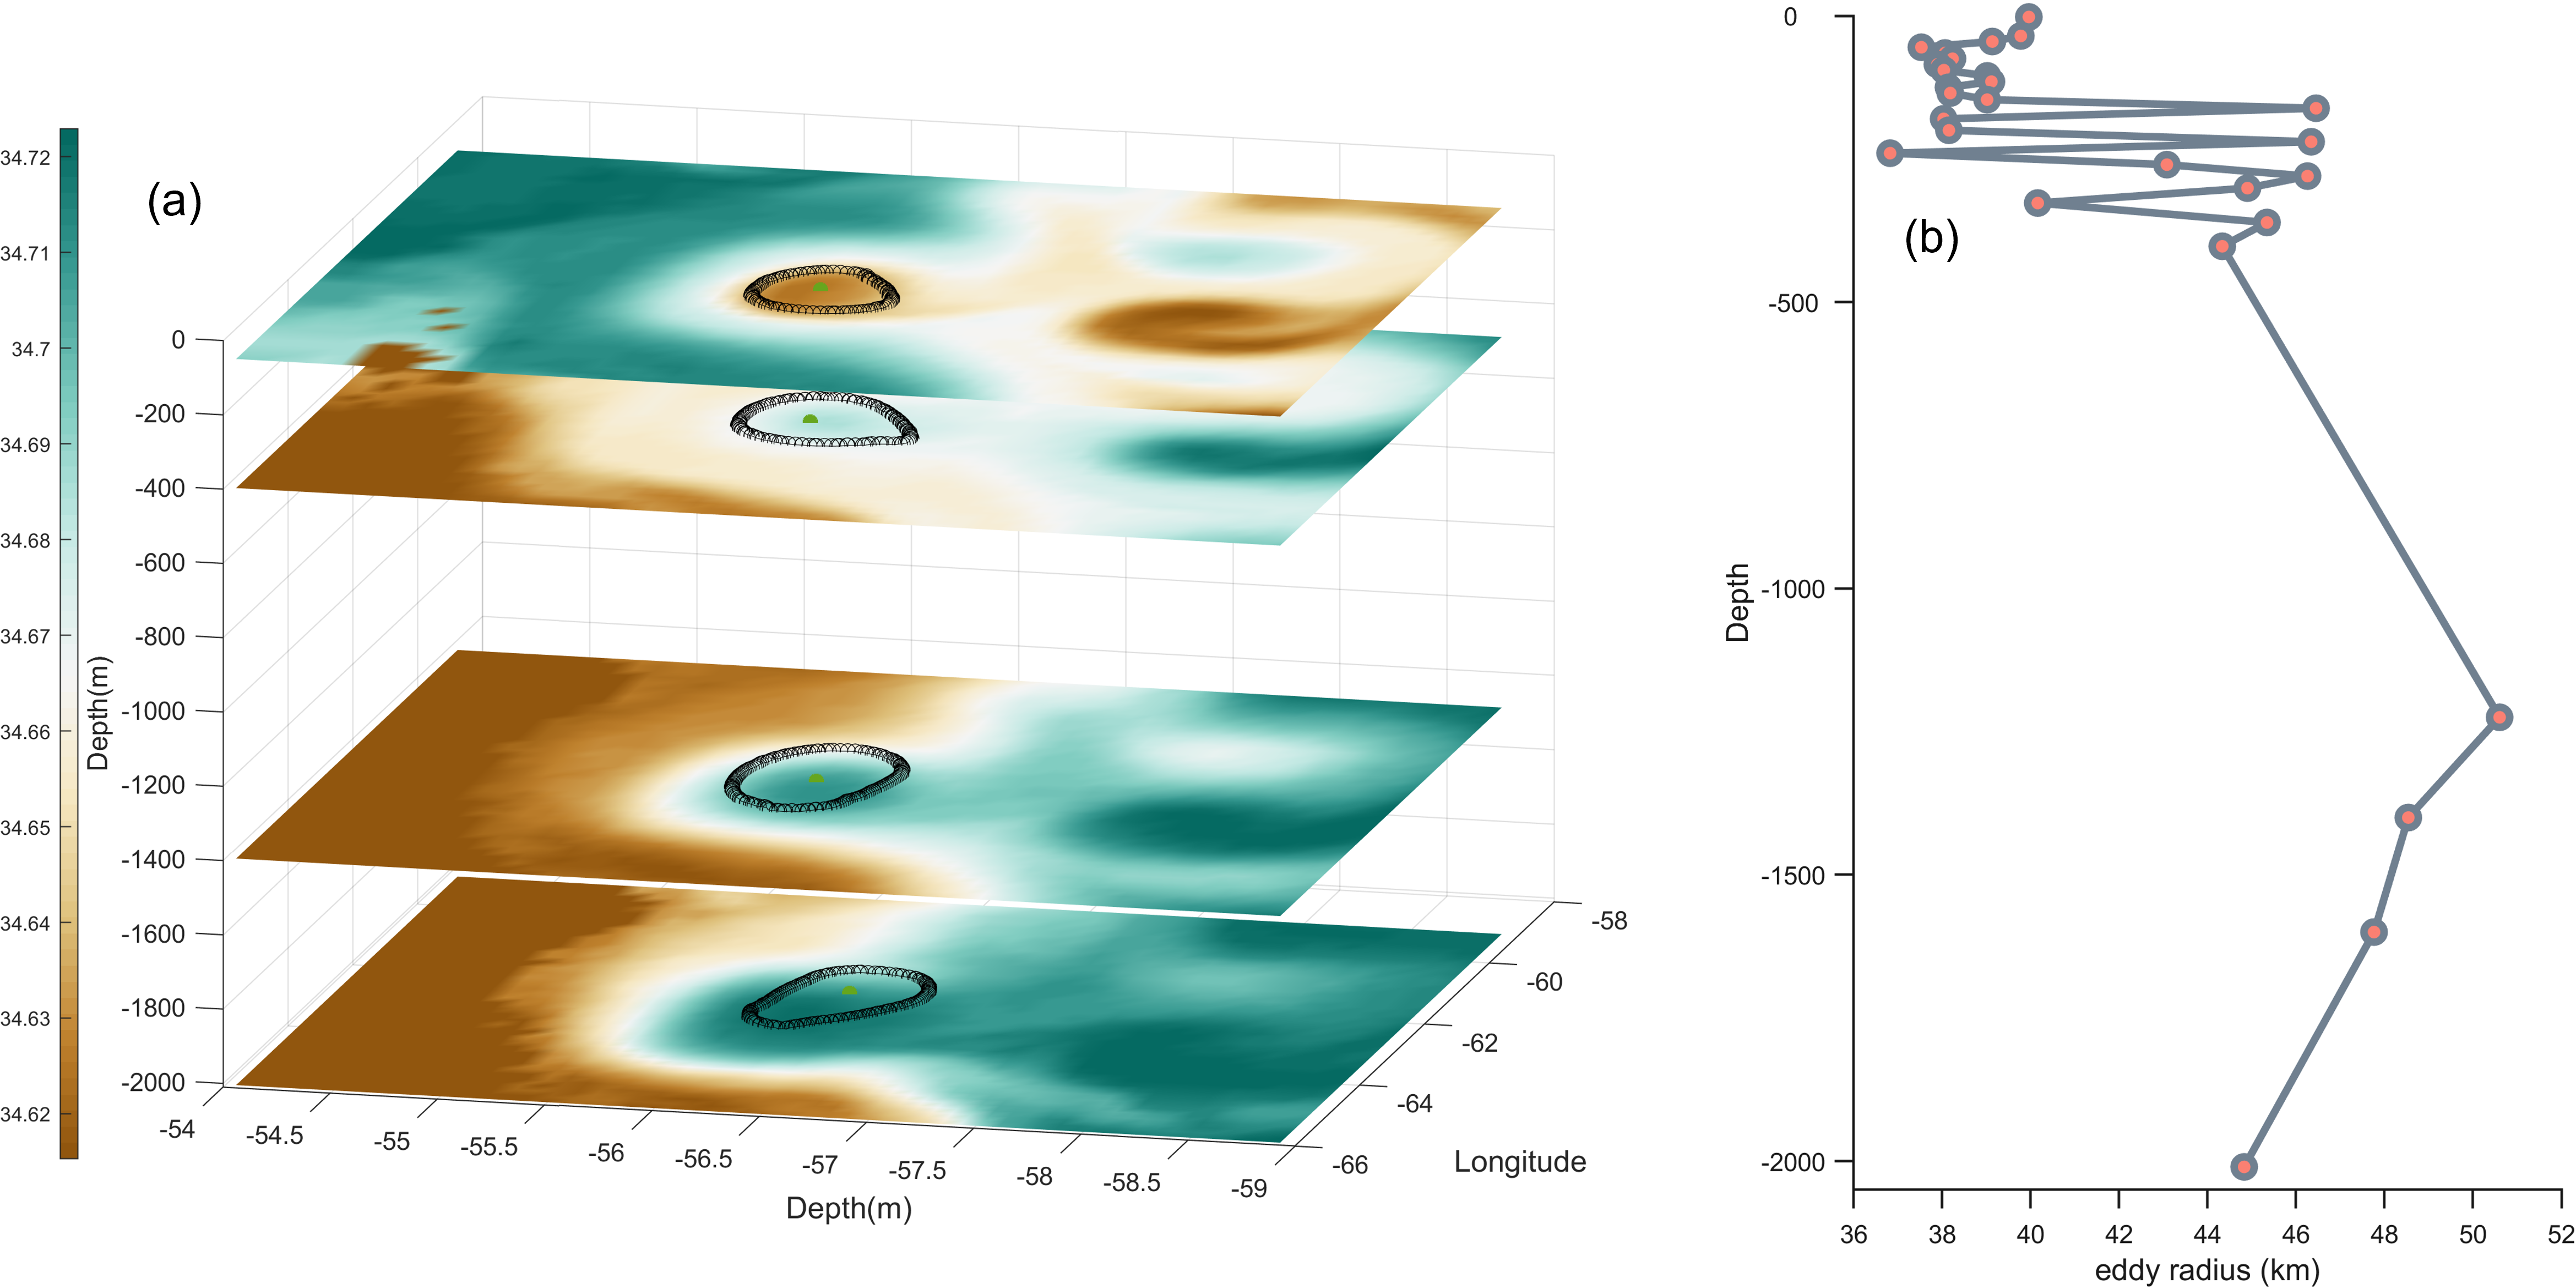
\includegraphics[width = 1\textwidth]{chapter/figure/cyclonic-3D.png}
    \caption{Vertical structure of a cyclonic eddy}
    \label{cyclonic-3D.png}
\end{figure}

\begin{figure}[htbp]
    \centering
    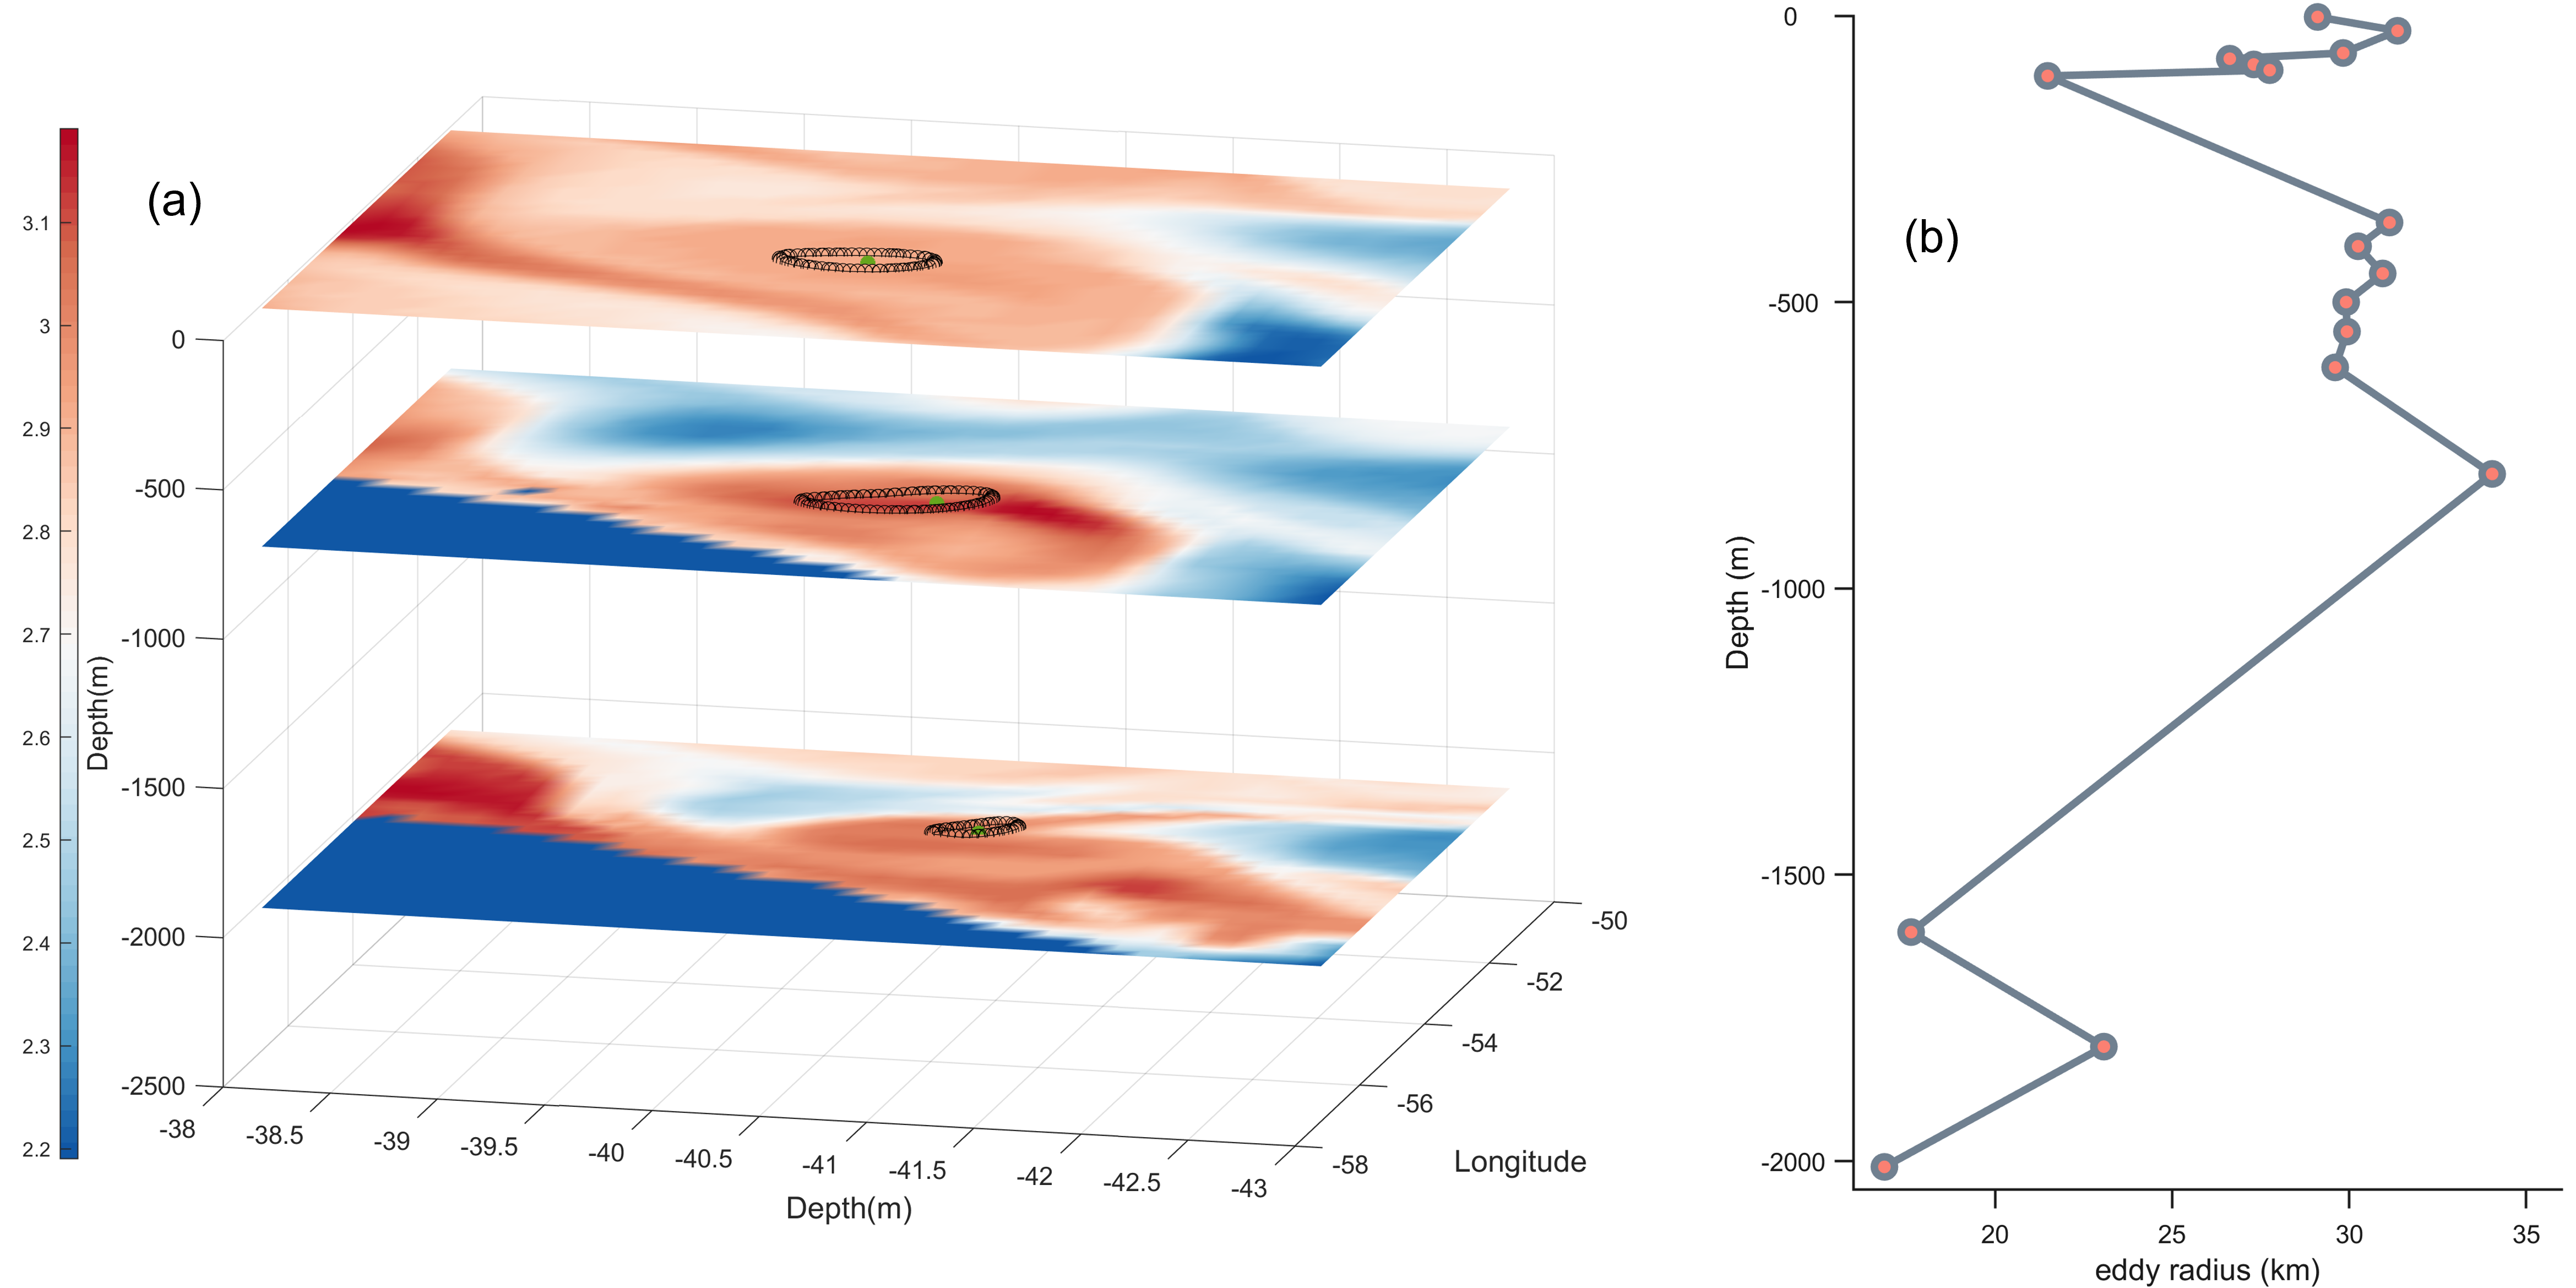
\includegraphics[width = 1\textwidth]{chapter/figure/2014-12-24_6.png}
    \caption{Vertical structure of an anticyclonic eddy}
    \label{2014-12-24_6.png}
\end{figure}

\clearpage

\section{Discussion and Conclusion}

Due to the limiting subsurface observational data, we build the three-dimensional structure of coherent eddies using model simulations. 

It is still questionable if we do capture the correct shape and penetration depth of coherent eddies and the visualization of propagation of three-dimensional eddies in the real oceanic flow is still on the way \cite{liu2018gulf}. We track surface eddies in this chapter and we attempt to trace the corresponding vortex signal in the subsurface. 

We have found three types of eddies in the study period (2013-2018), most of them are ens-shaped eddies having a maximum radius in the intermediate layer. Cyclonic eddies have the tendency to extend in the vertical direction. Eddies could alter the thermohaline properties of seawater: the cyclonic vortex is colder and saltier than the surrounding water column while the anticyclonic eddy is warmer and fresher.


\newpage

%\chapter{Eddies-induced transport in the Argentine Basin}

In this chapter, we present statistical analysis

\section{Introduction}

From the analysis result as shown in Chapter \ref{Eddies features analysis} and eddy vertical type in Chapter \ref{Three-dimensional eddies structures}, we gain insight into seasonal and annual change of surface eddy properties and eddy structure. However, more information about eddies' transport ability is needed to know because understanding water mass exchange of several important tracers (e.g., heat and salt) is crucial to eddy mixing and eddy parameterization \cite{guan2022seasonal}.

Volume, heat and salt transport carried by oceanic eddies are important source of water exchange especially in the Southern Ocean and Argentine basin. However, it is still under debate how much eddy-induced transport would contribute to the overall heat and salt transport and how it would change the local climate since most of the low-resolution climate models could not resolve eddies. In previous studies based on Eulerian methods, it is declared that eddy-induced zonal transport is comparable with the transports of wind-driven gyres and thermohaline circulation \cite{zhang2014oceanic} and eddy-induced meridional transport account for $20\%-30\%$ of the overall volume transport\cite{dong2014global}. However, studies based on Lagrangian approaches come to the conclusion that coherent eddy-induced material transport is smaller than Eulerian-based estimation by two magnitudes and its contribution to thermodynamics budget is less significant \cite{wang2015coherent}. 

Sea level anomaly from satellite can provides us with the mesoscale dynamical properties of mesoscale eddies; however, it could not give us subsurface information of eddies structures, let alone heat and salt transport induced by eddies. What is more, eddies-induced vertical movement of seawater can greatly deform the thermohaline structure and cause temperature and salinity anomalies inside eddies. Thus, it is of great importance to understand how eddies disturb the background salinity and temperature field and transport heat, salt and energy across the basin.

More importantly, eddies' crucial role in the large scale circulation and its distinct hydrographic properties compared with the surrounding waters influence a lot of oceanic processes such as energy cascade from mean kinetic energy (MKE) to eddy kinetic energy (EKE), upwelling or downwelling, etc.

According to the previous studies, eddy-induced mixing may contribute as much as the mean flow advection to the large-scale water mass subduction in Brazil–Malvinas Confluence region \cite{marshall2006estimates}.

\section{Estimate of eddy-induced heat and salinity transport}

There are currently three main Eulerian methods to calculate eddy-induced heat (salt) transport. The first one is direct calculation of the product of temperature (salt) anomaly and velocity anomaly $\overline{T^{\prime} V^{\prime}}\left(\overline{S^{\prime} V^{\prime}}\right)$ \cite{volkov2008eddy}. This approach requires long-term climate-state data to extract deviation from the mean field ($T = \overline{T}+ T^{\prime}$). Assuming a linear relationship between the temperature (salt) perturbation flux and the mean state field gradient, similar to the turbulent Reynolds stress relationship, thus avoiding deviated field calculations, we get the second estimation method: $\overline{T^{\prime} V^{\prime}} =k \frac{\overline{\partial T}}{\partial y}$ \cite{stammer1998eddy,chen2012eddy}. However, this estimation relies on the selection of an empirical eddy diffusion coefficient $k$.

Above methods still have their limitations because the Eulerian framework do not consider the the kinematic characteristics of the vortex as a whole. In fact, because of the highly nonlinear nature of the vortex, coherent eddy is different from the general perturbation. If we trace the vortex, the temperature and salt anomalies caused by the vortex will maintain a certain stability inside the vortex during its life cycle along the vortex trajectory. In other words, the temperature and salt anomalies can be carried and advected by vortex. This way of following the vortex trajectory can only be clearly and precisely described in the Lagrangian framework.


\section{Eddy-induced heat transport}

\section{Eddy-induced salt transport}

eddies fresher isopycnal layer salinity anomalies

all the screened eddies

\section{Eddies-eddies interaction and eddies-mean flow interaction}

From eddies footprint, we could conclude that eddies absorb into Brazil Current.

\newpage

%\chapter{Comparison of different eddy detection methods}\label{sec-eval}

In this chapter, we evaluate the robustness of the Lagrangian method by comparing the eddy detecting results between SSHA Eulerian method (as illustrated in figure \ref{A schematic SSHA anticyclonic eddy}) and the LAVD method.

\section{Introduction of Mesoscale Eddy Trajectory Atlas}

We download \href{https://www.aviso.altimetry.fr/en/data/products/value-added-products/global-mesoscale-eddy-trajectory-product/meta2-0-dt.html}{Eulerian eddies trajectories data}  from AVISO+, which detected eddies from Sea Level Anomaly field of merged altimetry datasets using SSHA method as described in chapter \ref{Eulerian methods} and told us information of type, speed, and radius of Eulerian eddies globally \cite{chelton2011global}. This dataset contains eddies with a life cycle of more than 4 weeks. The time frame of the dataset is from 1993 to the present. In this chapter, all the eddies in the spatial range 70°W to 30°W, 60°S to 30°S are used for the statistical analysis of Eulerian eddies. The time range of the vortex dataset selected for the study is from January 1993 to December 2019.


\section{Statistics results of Eulerian detection method}


The statistics Eulerian detection results are shown below in figure \ref{anticyclonic eddies numbers from 1993 to 2019} and figure \ref{cyclonic eddies numbers from 1993 to 2019} (we separate the research region into $1^\circ \times 1^\circ$ sub-domain and sum up the eddies appearing respectively in each sub-domain). From 1993 to 2019, 13683 eddies were generated in the whole region, 6686 of them are anti-cyclonic eddies and 6997 are cyclonic ones. Among all the eddies, along the coast of South America, only a few eddies were detected, which is consistent with Lagrangian methods. In the northern part and the southwest part of the Argentine Basin, we observe vast numbers of eddies. In the center part of the Argentine Basin, only a few eddies were detected. Many vortices have been observed in the Southern Ocean region or in the connecting water region between Argentine Basin and the Southern Ocean near the islands. The general pattern is quite similar to the results in the chapter \ref{Eddies features analysis} when the Lagrangian method is adopted although the Eulerian method could detect a higher number of eddies.

\begin{figure}[ht]
  \centering
  \setlength{\abovecaptionskip}{0.cm}
  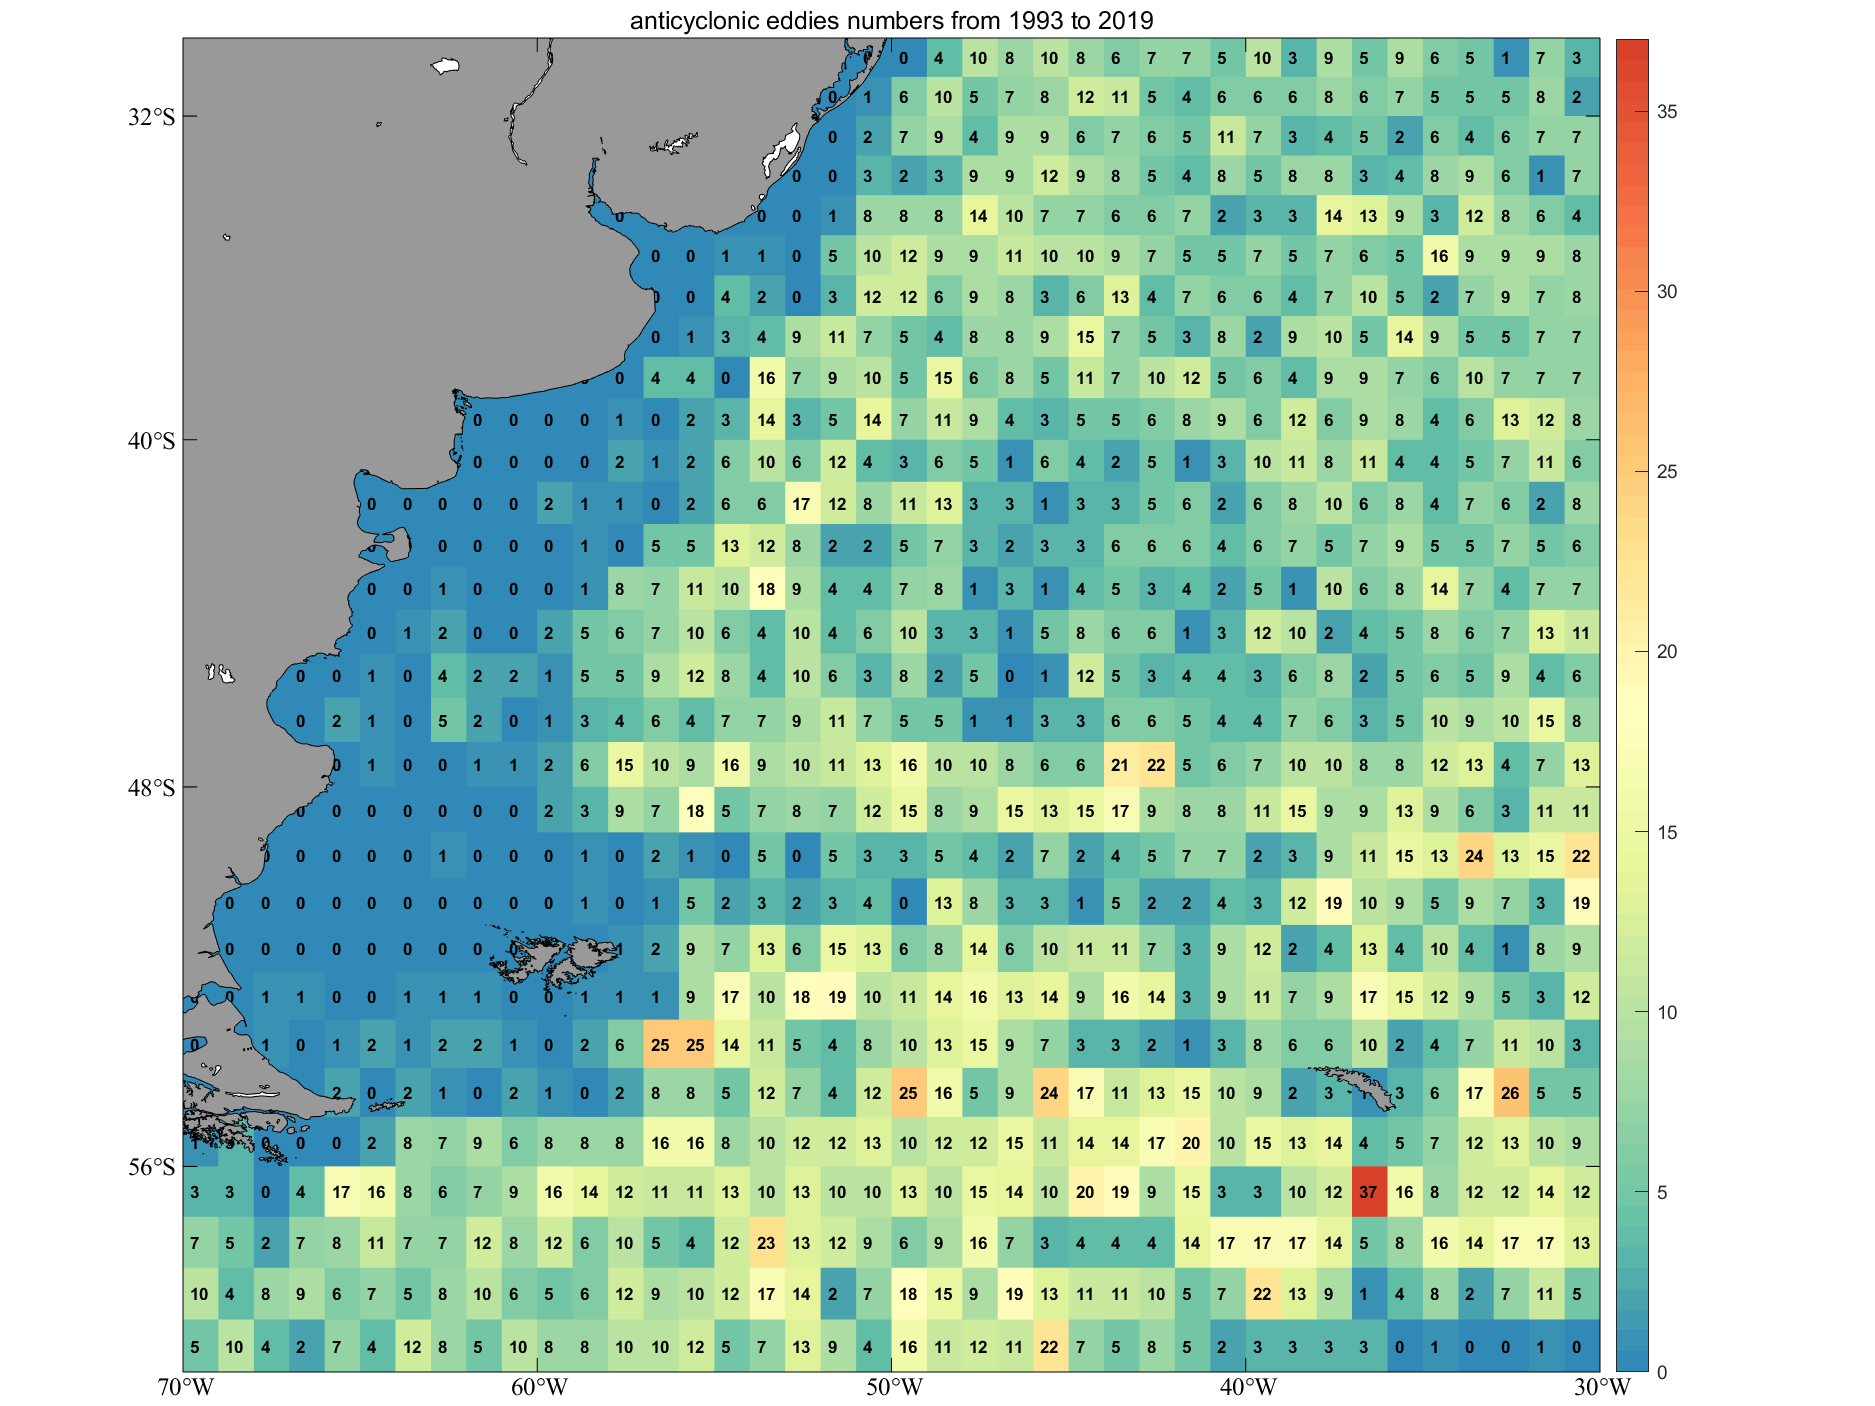
\includegraphics[width=15cm]{chapter/figure/anticyclonic eddies numbers from 1993 to 2019.png}
  \caption
  {Anticyclonic eddies numbers from 1993 to 2019}
  \label{anticyclonic eddies numbers from 1993 to 2019}
\end{figure}

\begin{figure}[ht]
  \centering
  \setlength{\abovecaptionskip}{0.cm}
  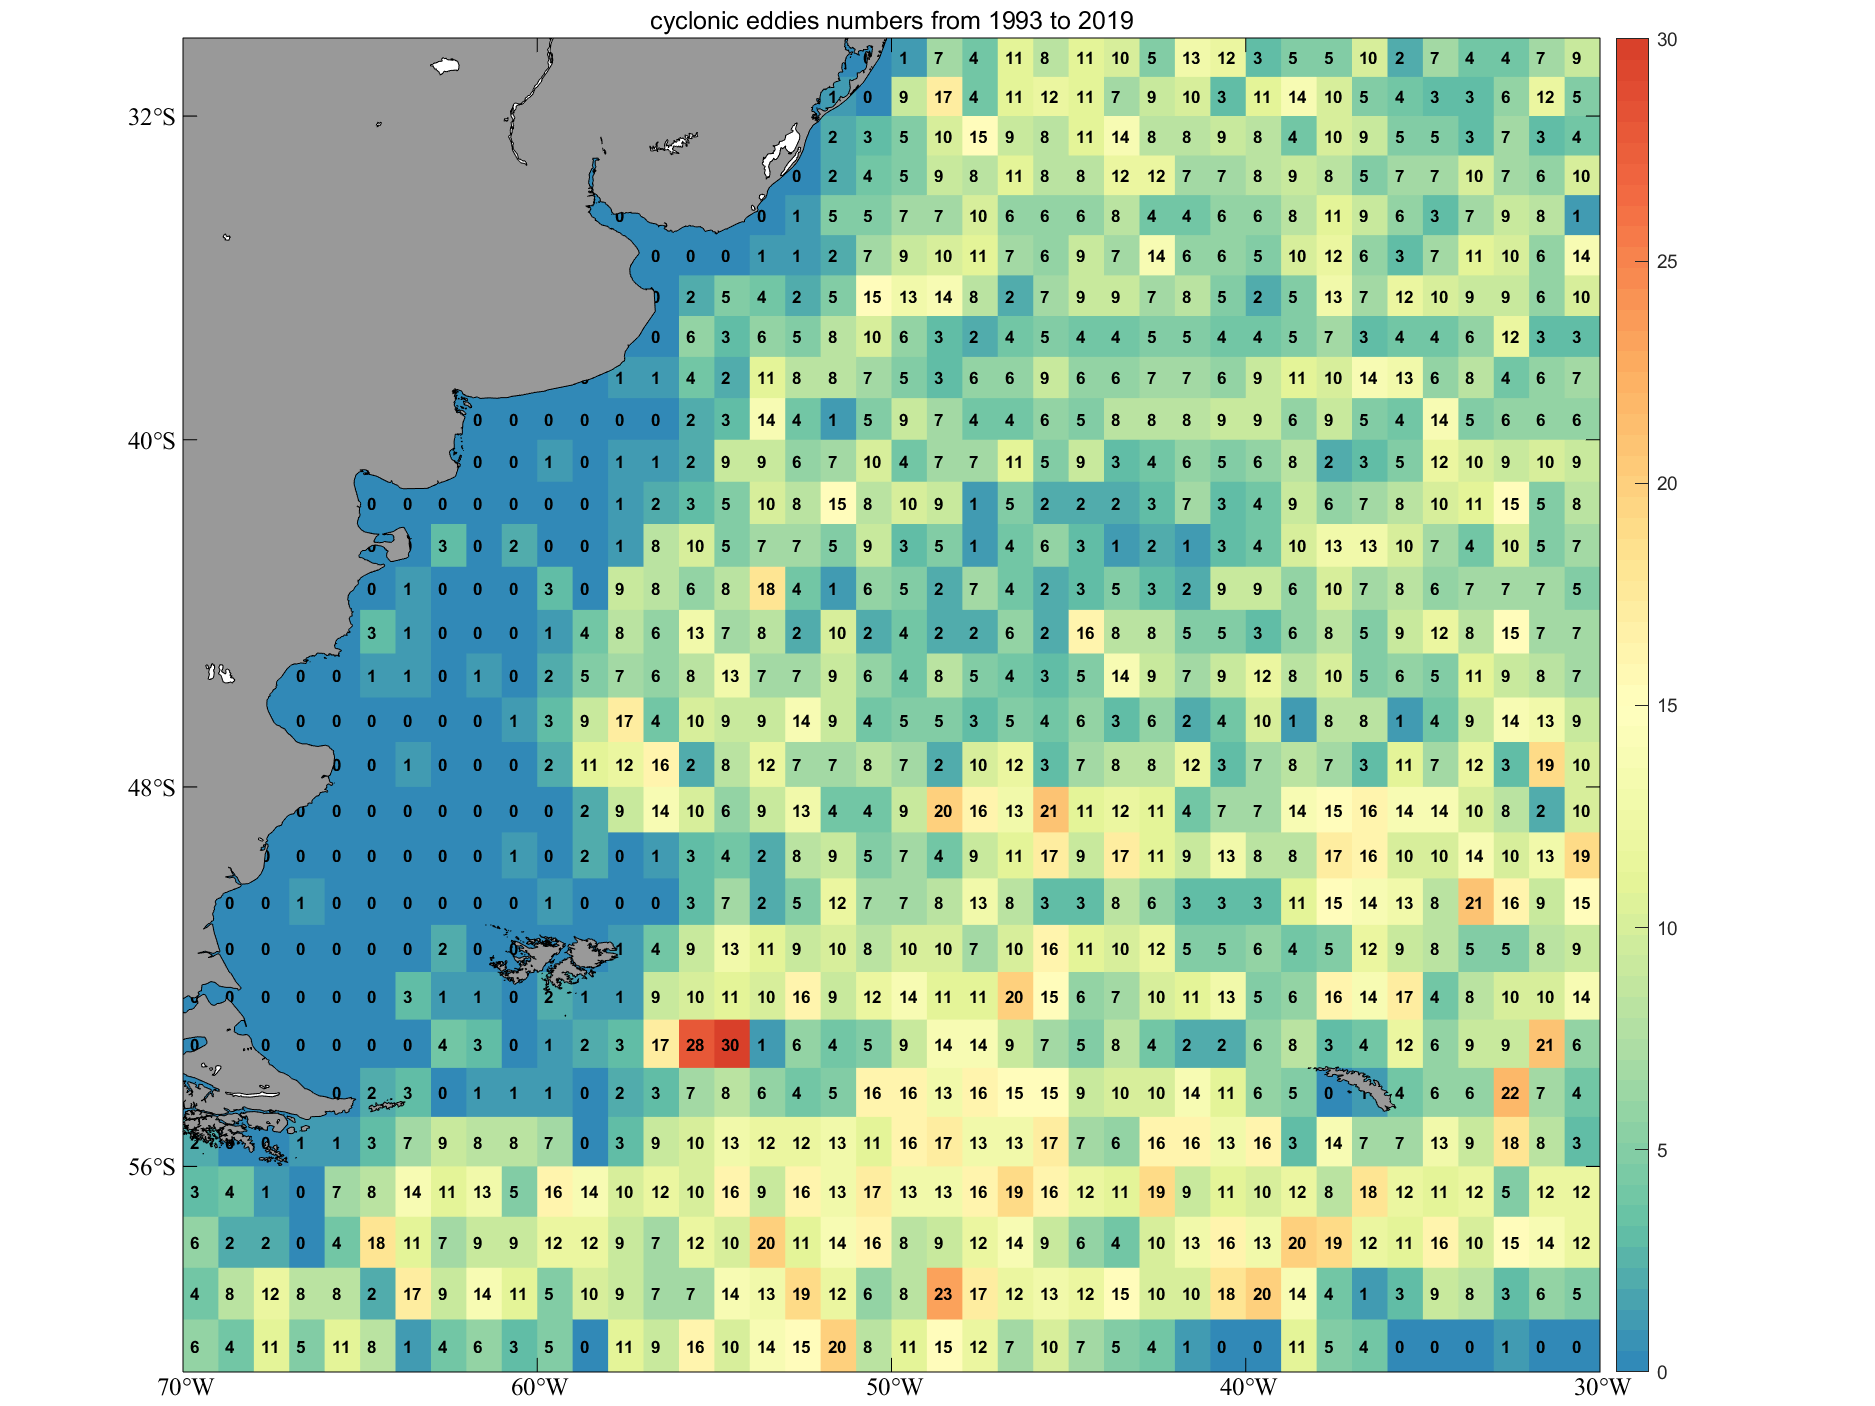
\includegraphics[width=15cm]{chapter/figure/cyclonic eddies numbers from 1993 to 2019.png}
  \caption
  {Cyclonic eddies numbers from 1993 to 2019}
  \label{cyclonic eddies numbers from 1993 to 2019}
\end{figure}

The following figures \ref{Anticyclonic eddies trajectories} and \ref{10 Cyclonic eddies trajectories} are the trajectories map of anticyclonic eddies and cyclonic eddies with lifetimes longer than 30 days. In order not to overlap the trajectories with each other, only one-tenth of the total eddies are selected and plotted on the map.


\begin{figure}[ht]
  \centering
  \setlength{\abovecaptionskip}{0.cm}
  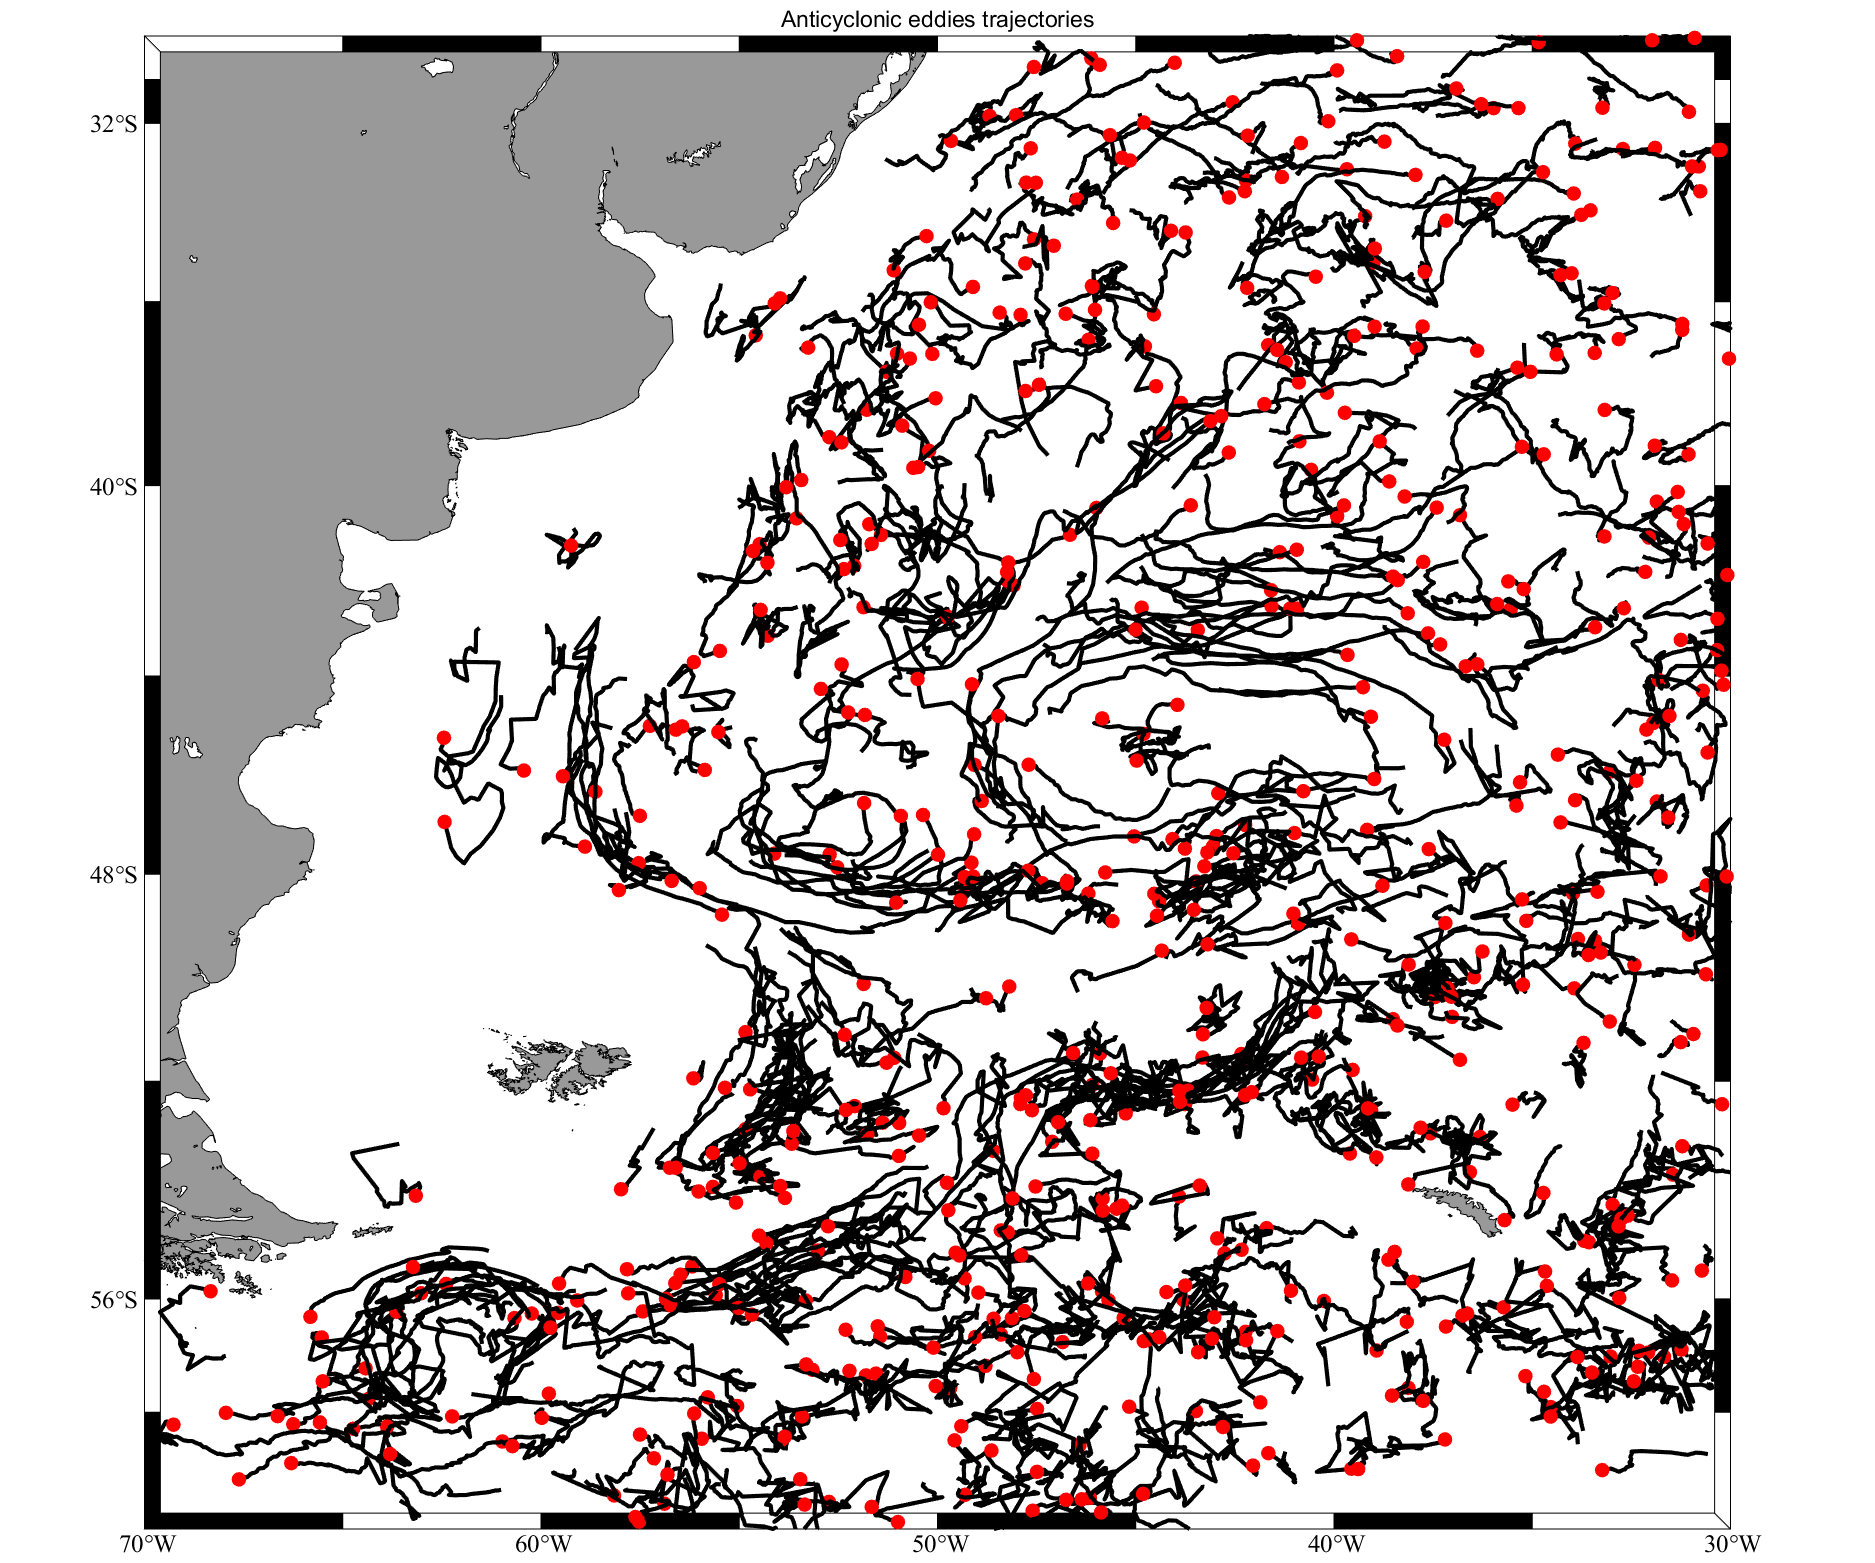
\includegraphics[width=1.0\textwidth]{chapter/figure/10 Anticyclonic eddies trajectories.png}
  \caption
  {Anticyclonic eddies trajectories from 1993-2018}
  \label{Anticyclonic eddies trajectories}
\end{figure}

\begin{figure}[ht]
  \centering
  \setlength{\abovecaptionskip}{0.cm}
  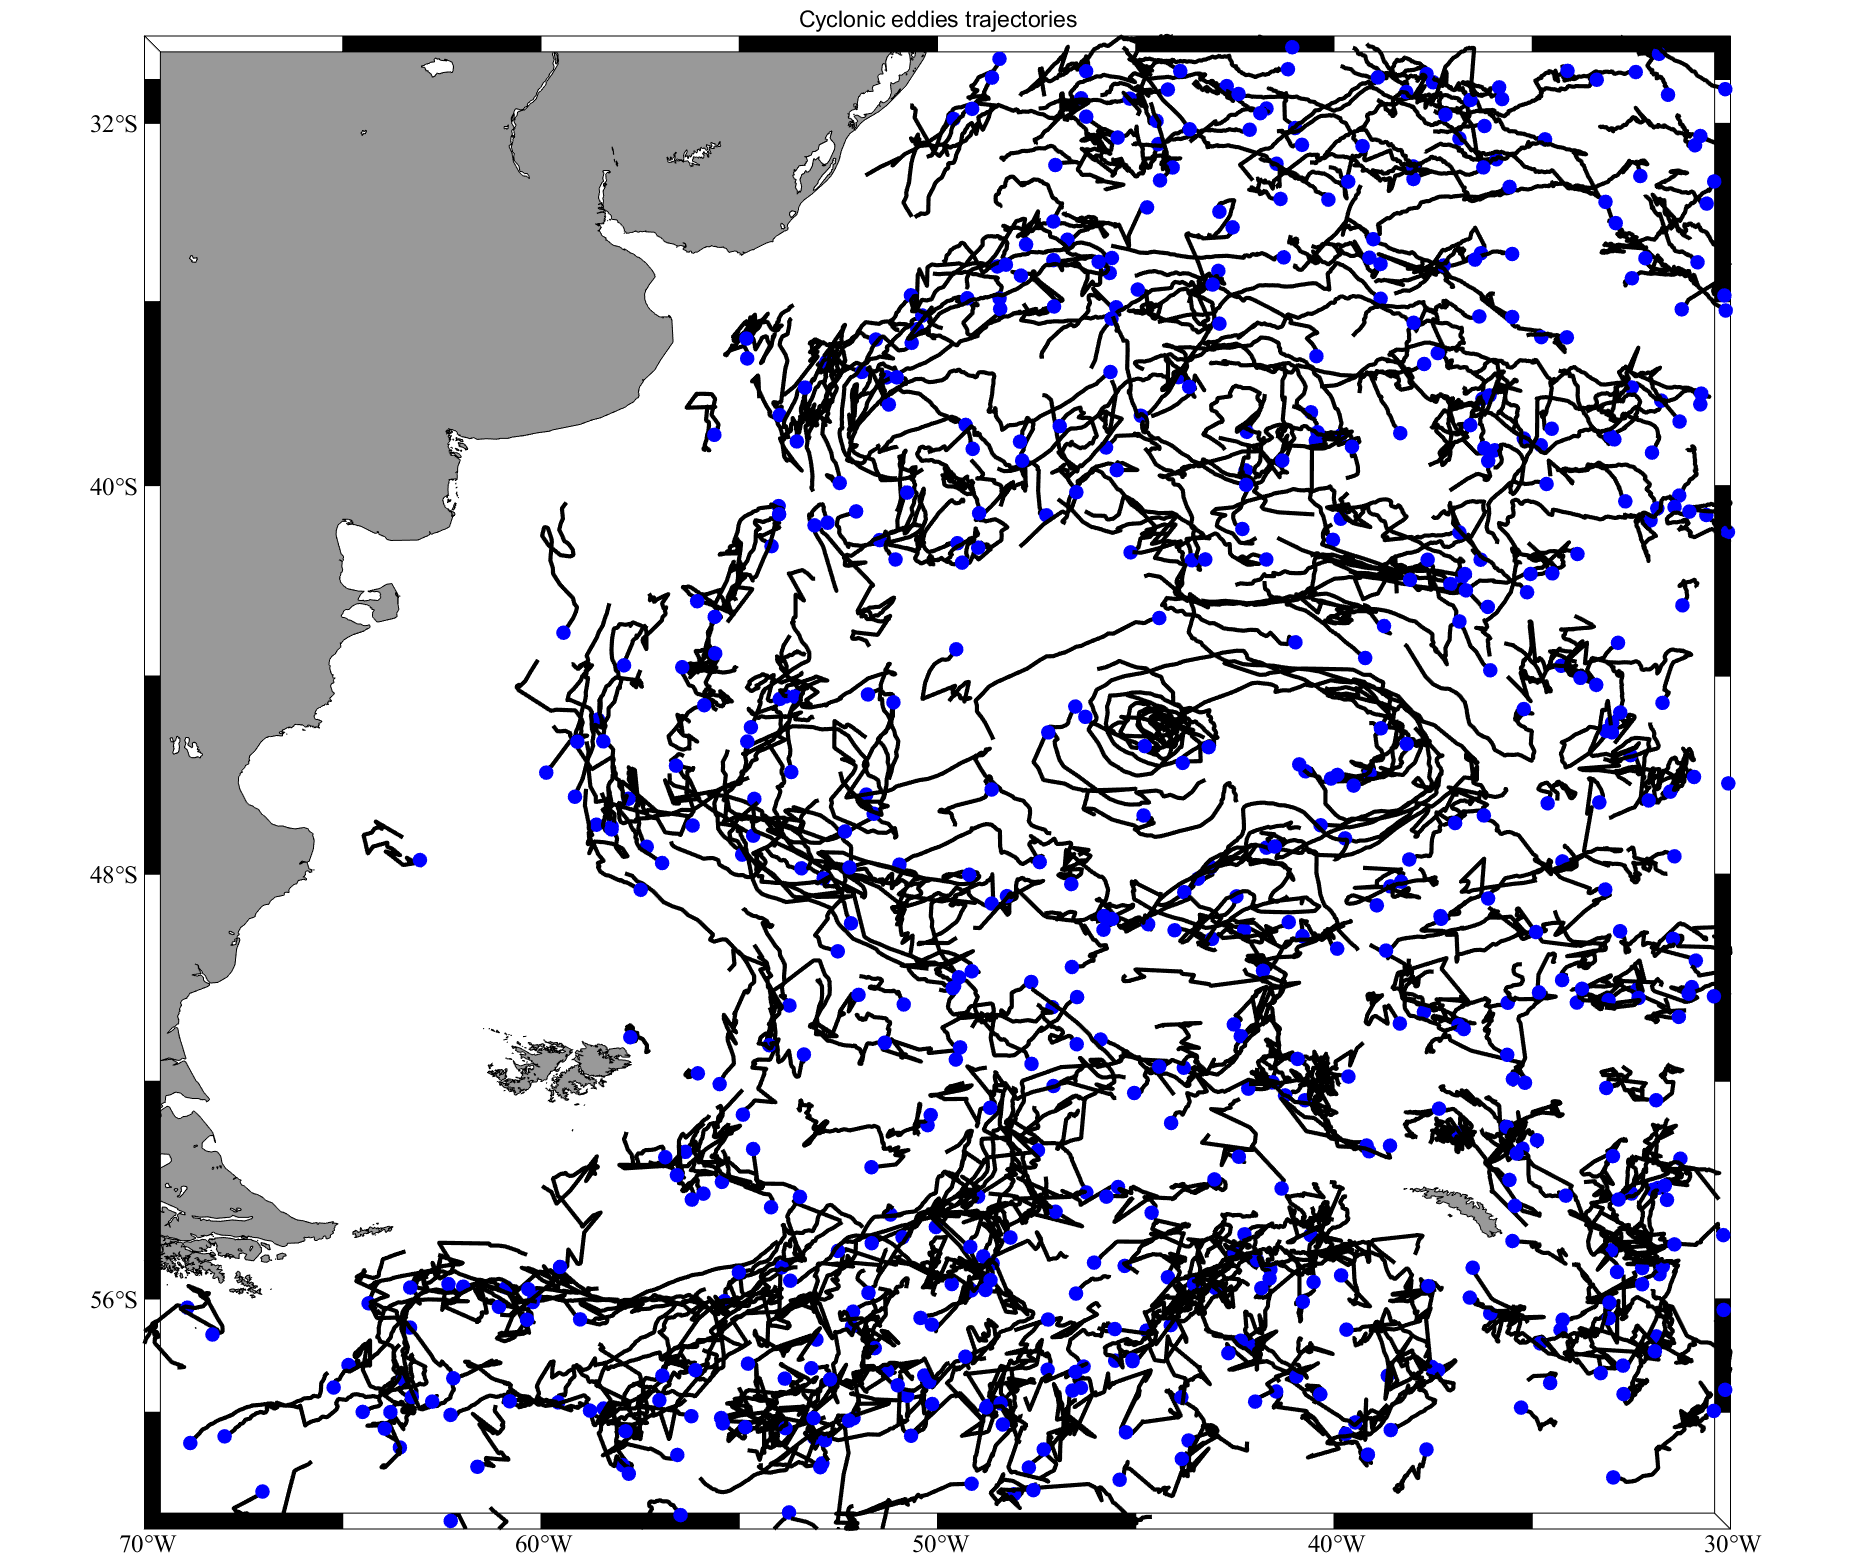
\includegraphics[width=1.0\textwidth]{chapter/figure/10 Cyclonic eddies trajectories.png}
  \caption
  {Cyclonic eddies trajectories from 1993-2018}
  \label{10 Cyclonic eddies trajectories}
\end{figure}


From figure \ref{Eulerian eddy number} , the observed temporal distribution of Eulerian eddies suggests that about 200-300 eddies would be generated in the Argentine Basin each year and the number of eddies decreases a little bit in recent years.
Eddies number distributes unevenly in the four-season: in summer, more eddies would appear and fewer eddies would be generated in winter. This pattern is similar to the results found in chapter \ref{Eddies features analysis}. The number of cyclonic eddies outweighs that of anticyclonic eddies by about 5\%.

The radius of Eulerian eddies is about 70 km, and anticyclonic eddies are a little bigger than cyclonic ones. The result is about twice as large as the Lagrangian eddy, which implies that Eulerian detection method may outweigh coherent transport carried by oceanic eddies and the outer part of Eulerian eddies was not so robust.

\begin{figure}[ht]
  \centering
  \setlength{\abovecaptionskip}{0.cm}
  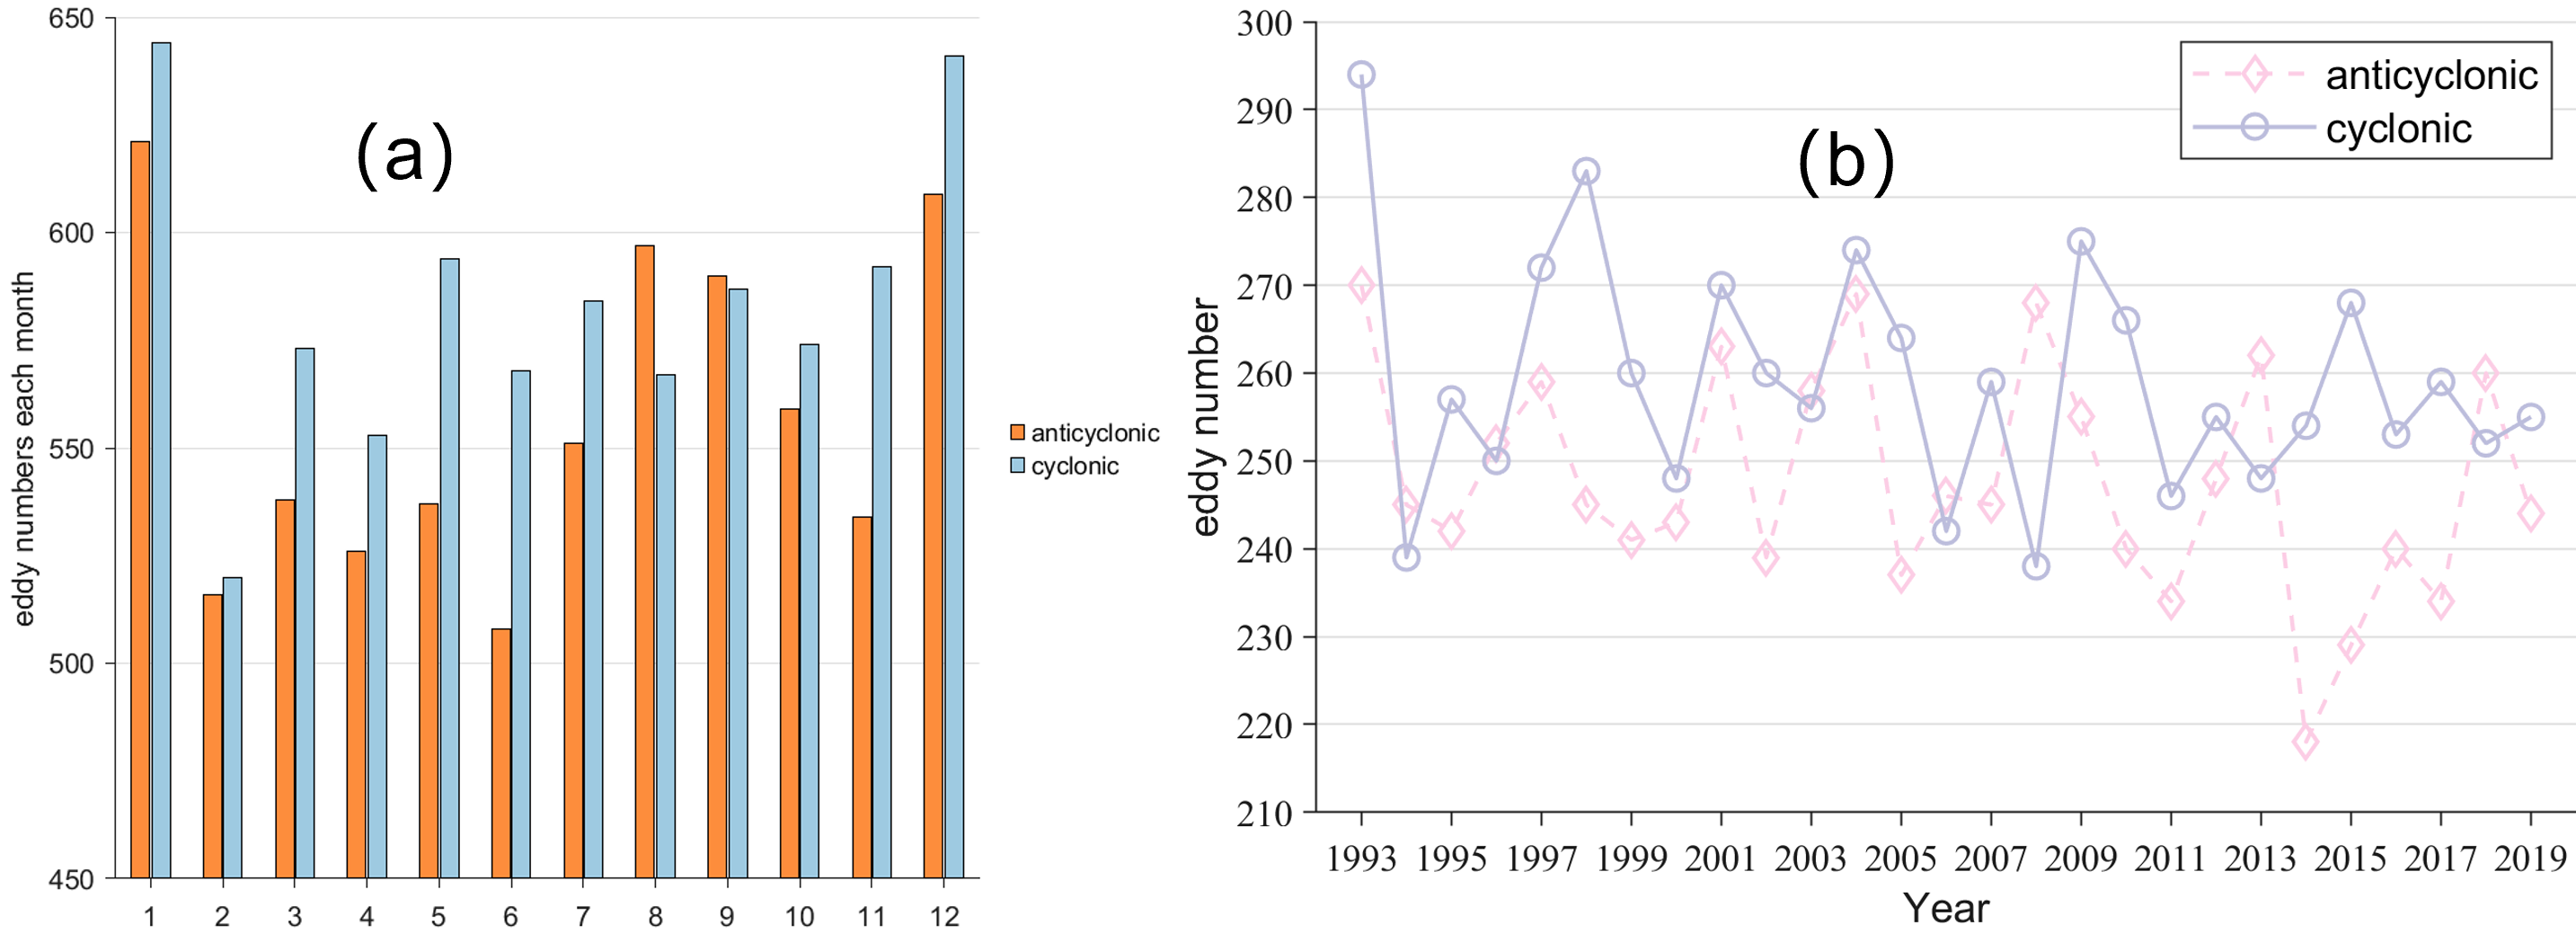
\includegraphics[width=15cm]{chapter/figure/Eulerian eddy number.png}
  \caption
  {Monthly and annual volume change characteristics of Eulerian eddy}
  \label{Eulerian eddy number}
\end{figure}


\begin{figure}[ht]
  \centering
  \setlength{\abovecaptionskip}{0.cm}
  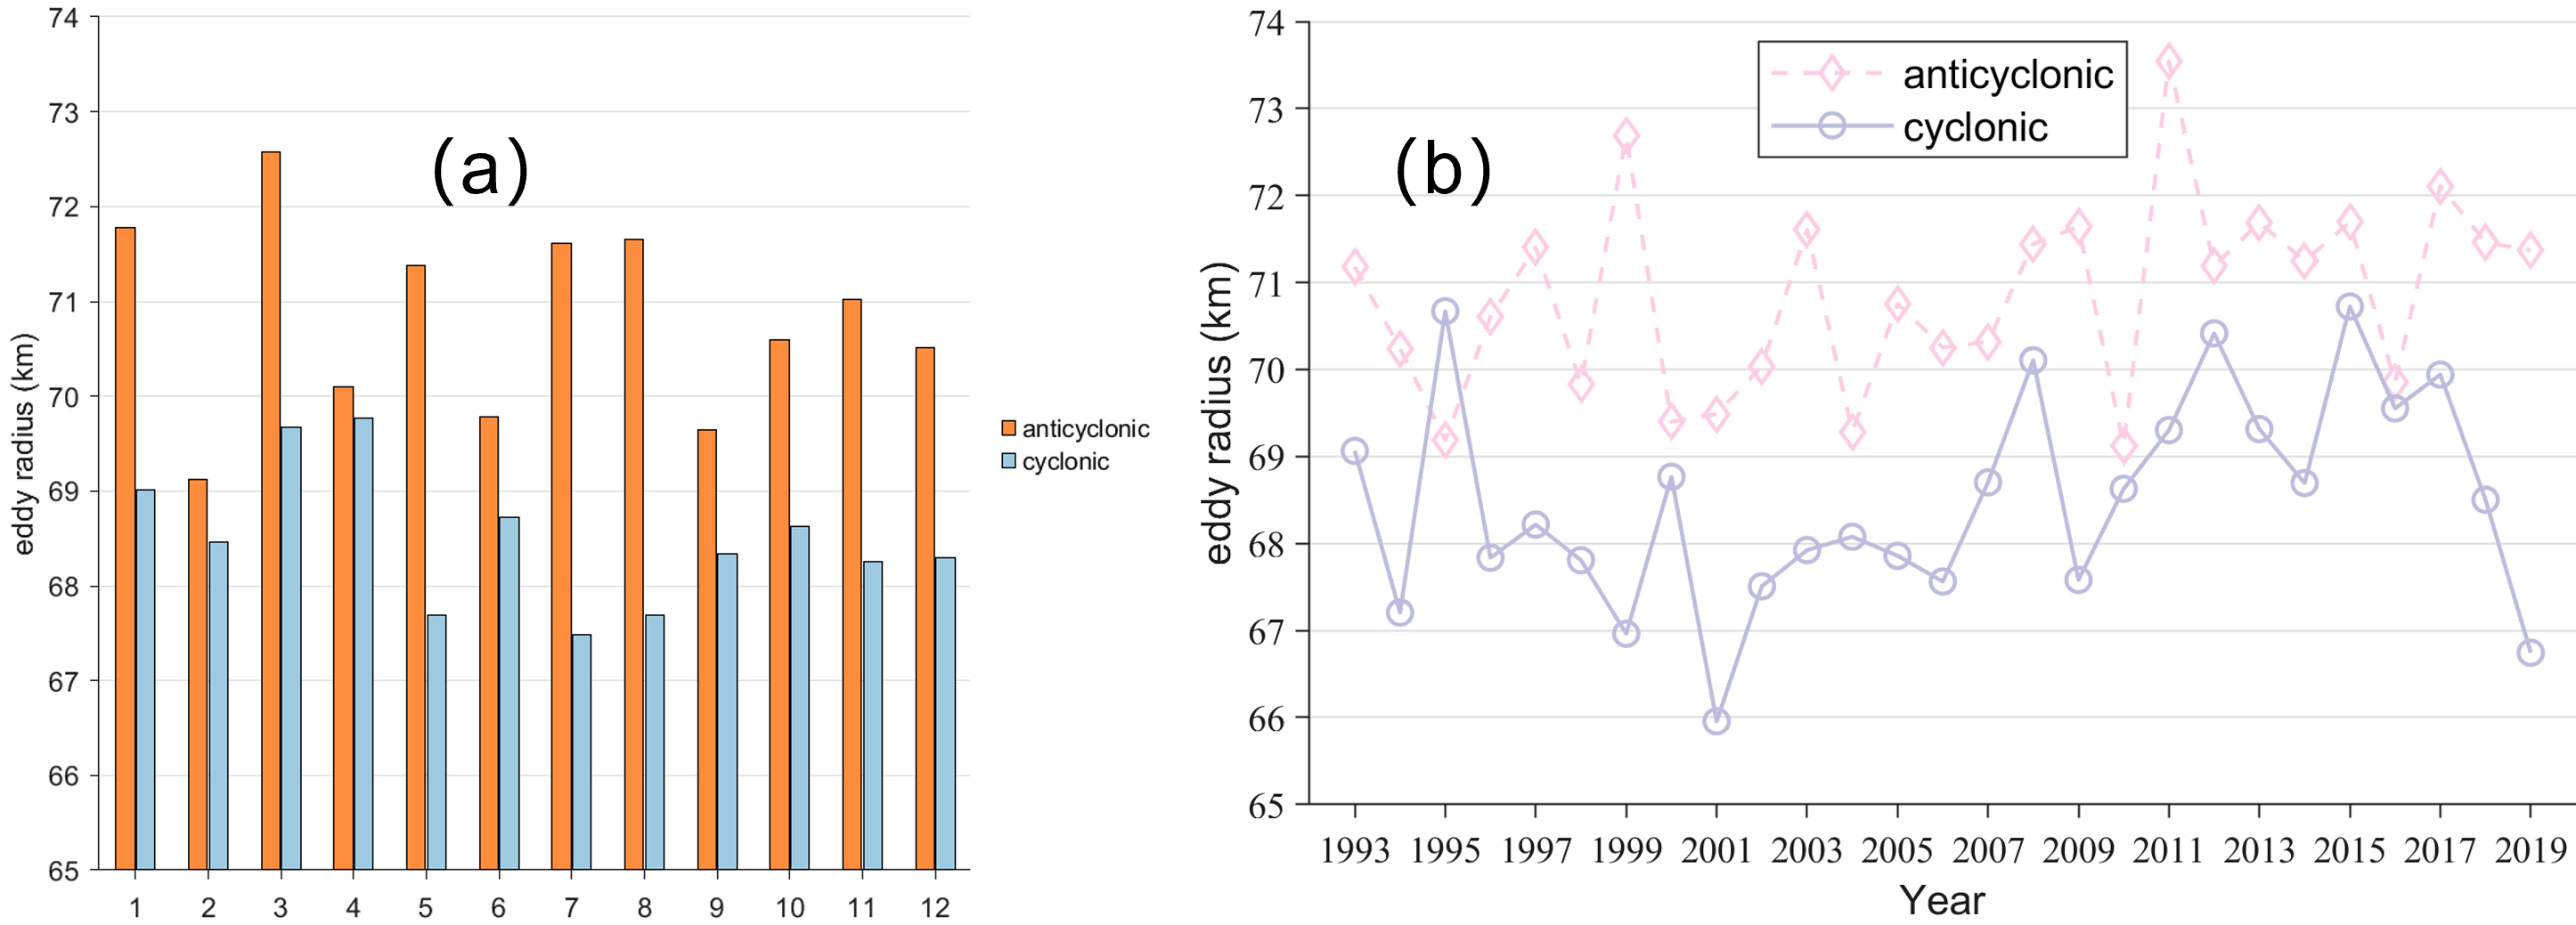
\includegraphics[width=15cm]{chapter/figure/Eulerian eddy radius.png}
  \caption
  {Seasonal and annual variation of Eulerian eddy number and radius}
  \label{Eulerian eddy radius}
\end{figure}


Figure \ref{Cyclonic eddy lifetime Frequency} and \ref{Anticyclonic eddy lifetime Frequency}
show the life estimation of Eulerian eddies, eddies with life estimation ranging from 30 to 60 days occupies 61\% of the entire number of vortexes while eddies with lifetime shorter than 30 days only account for 8\% and eddies with life-range over 180 days only takes up 1.5\% (1.6\% in cyclonic eddies and 1.4\% in anticyclonic eddies). The most long-living eddy lasted for 308 days. Thus, choosing 30 days as the coherent time for LAVD methods is convincing. 

\begin{figure}[ht]
  \centering
  \setlength{\abovecaptionskip}{0.cm}
  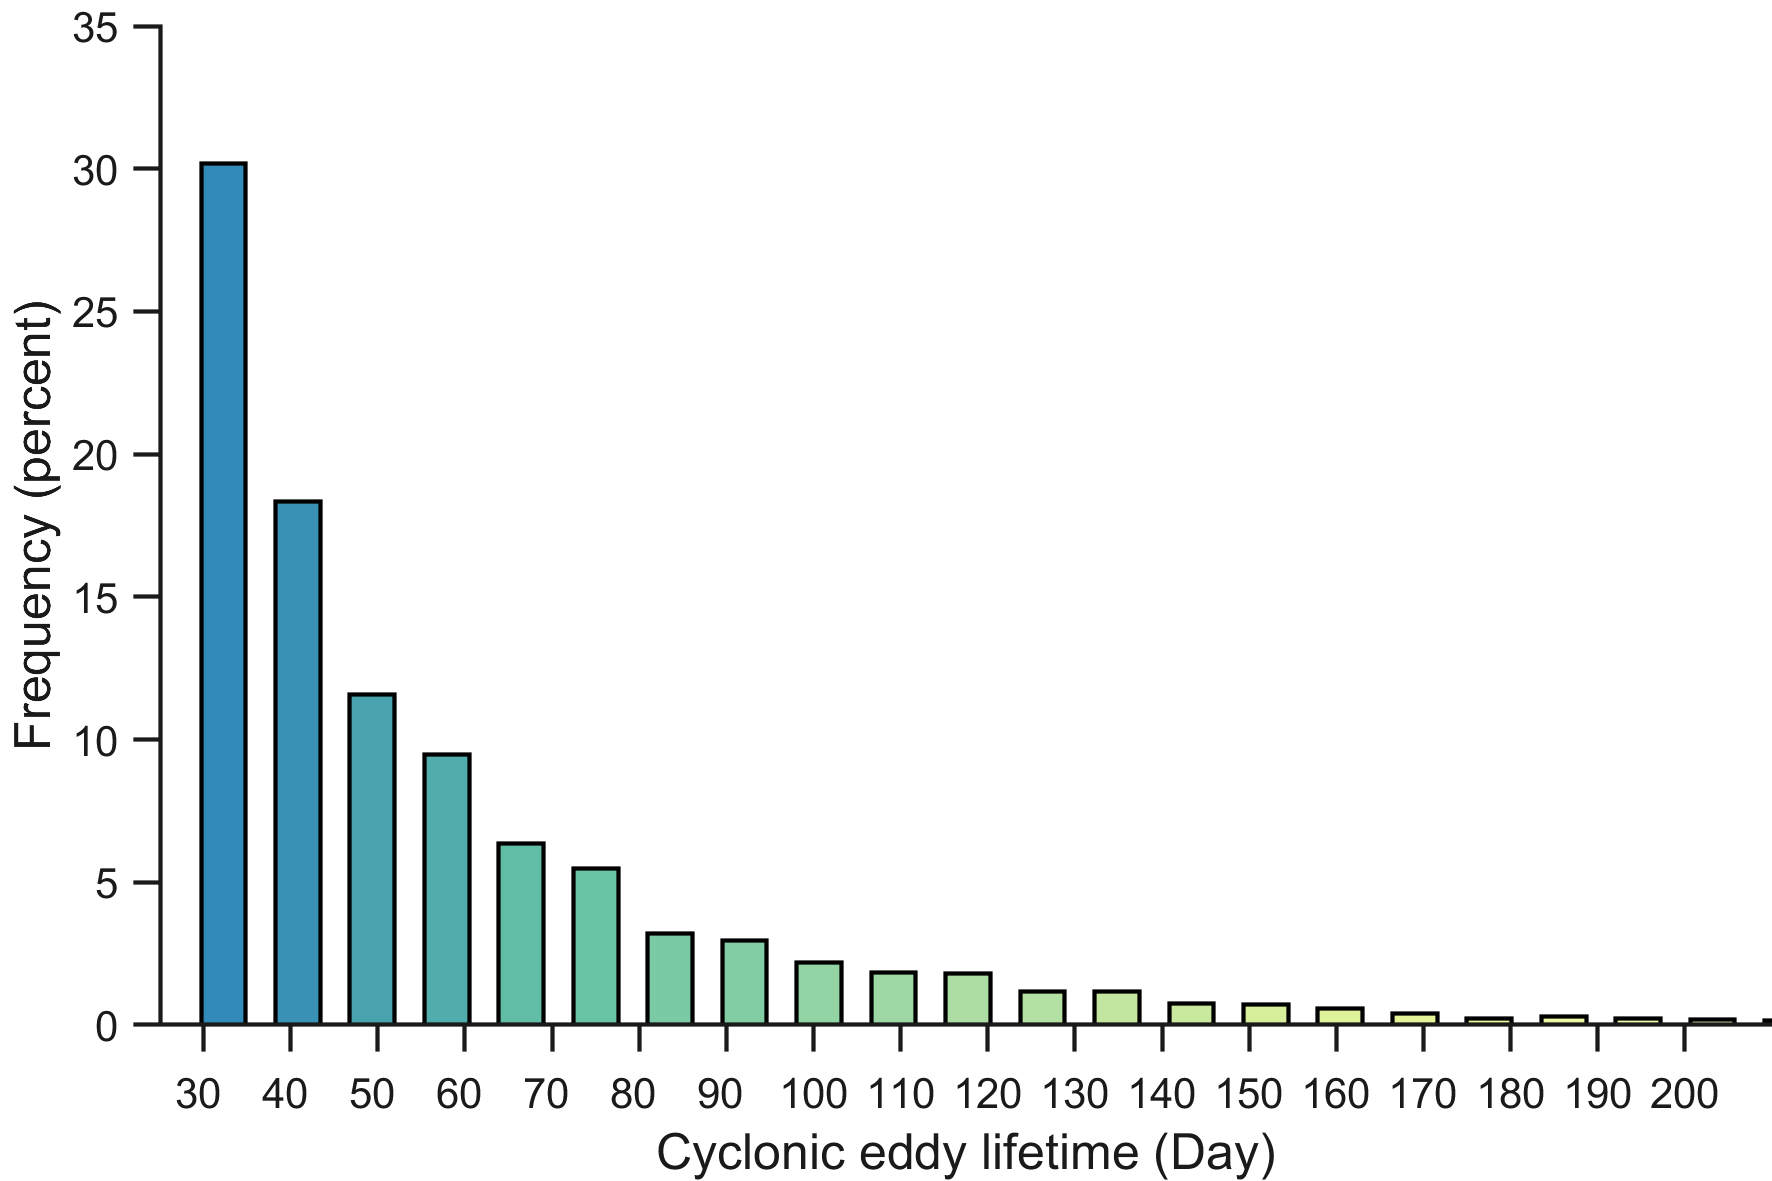
\includegraphics[width=15cm]{chapter/figure/Cyclonic eddy lifetime Frequency.png}
  \caption
  {Cyclonic Eulerian eddy lifetime Frequency}
  \label{Cyclonic eddy lifetime Frequency}
\end{figure}

\begin{figure}[ht]
  \centering
  \setlength{\abovecaptionskip}{0.cm}
  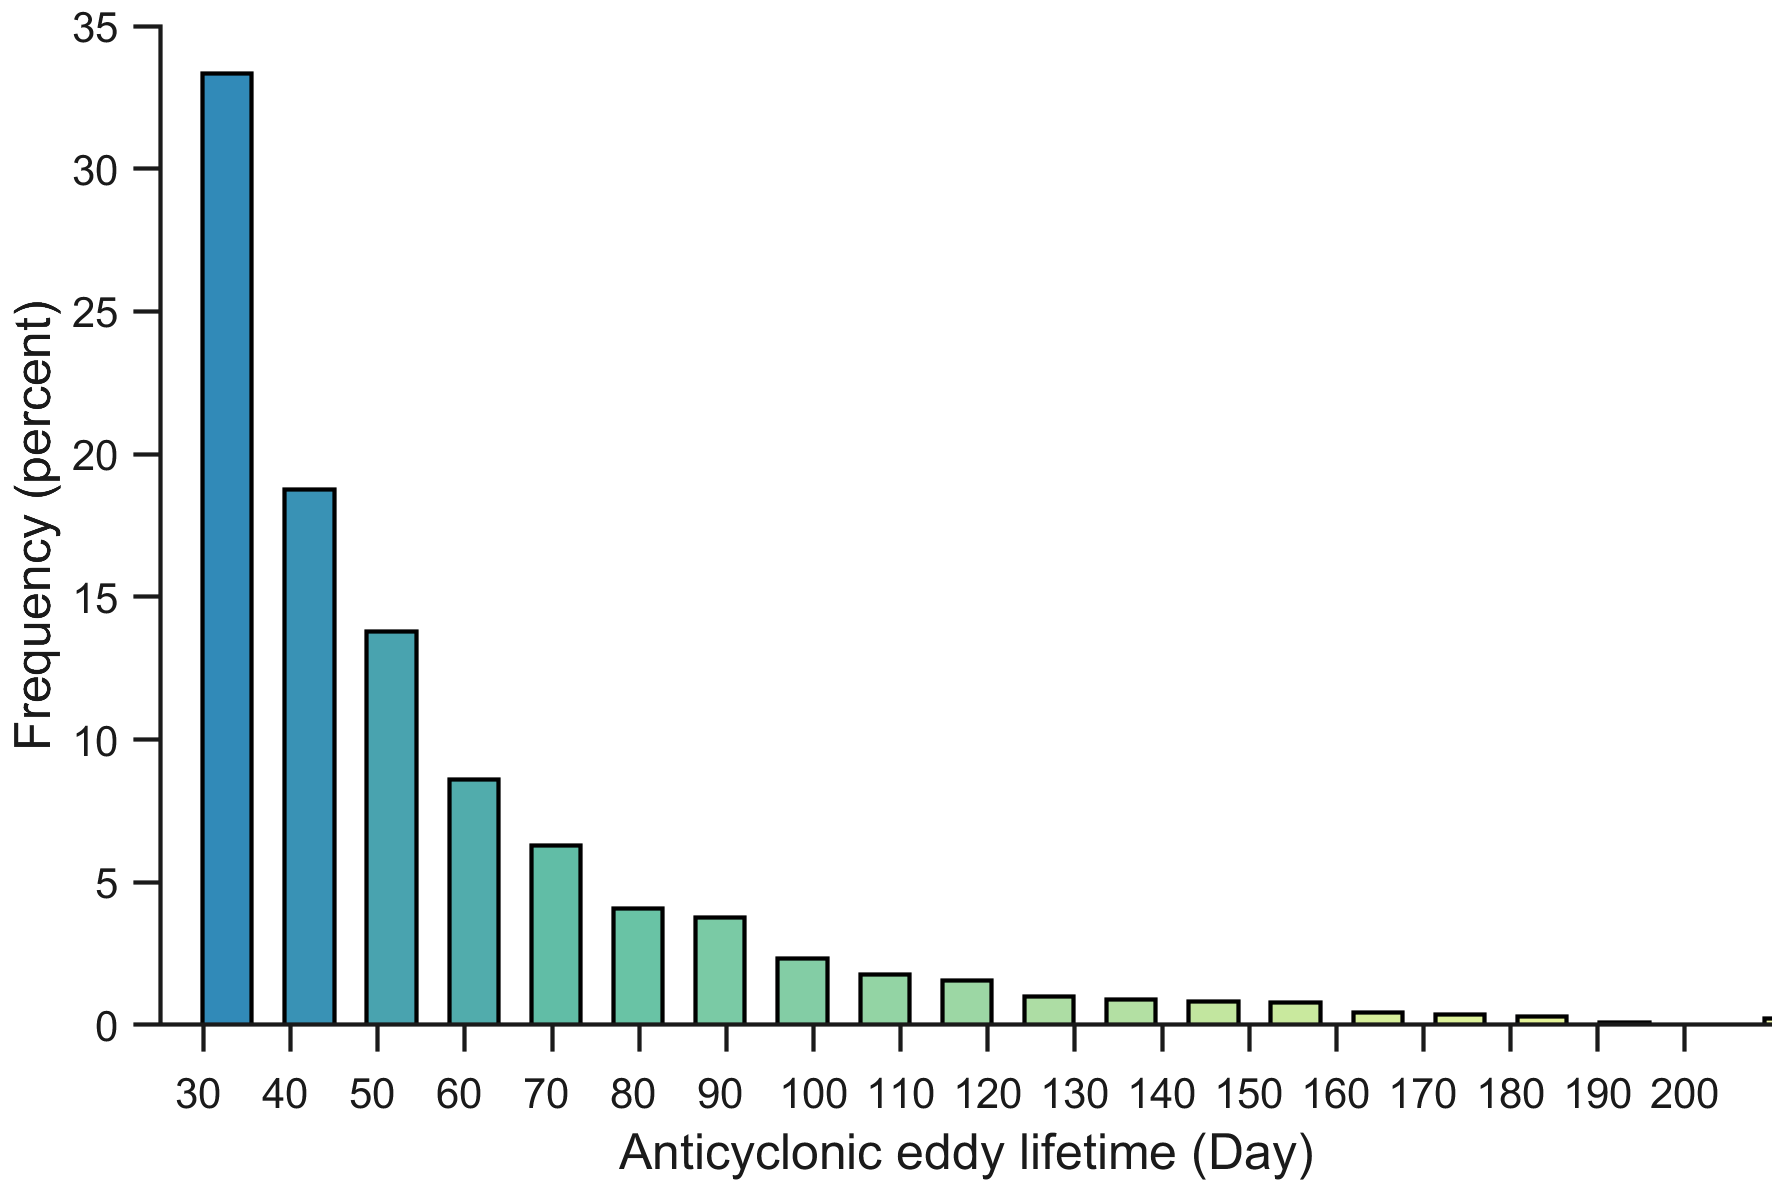
\includegraphics[width=15cm]{chapter/figure/Anticyclonic eddy lifetime Frequency.png}
  \caption
  {Anticyclonic Eulerian eddy lifetime Frequency}
  \label{Anticyclonic eddy lifetime Frequency}
\end{figure}

\section{Comparison of Lagrangian and Eulerian methods}

Since we adopt different methods to detect eddies, it is necessary to test the robustness of the results.


Search through the whole eddies dataset, we have found an Eulerian eddy that originated from 04-Aug-2006 and lasted for 140 days and the corresponding Lagrangian eddy has $t_0 = 2014-09-01$ and a coherent time of 120 days.

Figure \ref{coherence of eddy} shows the evolution process of this selected vortex (x label represents the lontitude and y label represents the latitude). In the figure, the coherent Lagrangian eddy part is marked in red, the blue dots represent the area enclosed by the Eulerian eddy, and the black ring shows the particle outside of the Eulerian eddy. We release the particles and find that the Eulerian eddy could maintain the overall shape in the first 15 days and then the outer part of the Eulerian eddy would deform and stretch in the evolution process. After 70 days, two fluid arms are flung from the core of the Euler vortex and 100 days later, only part of the blue particle is still inside the Eulerian vortex. However, the LAVD Lagrangian eddy still maintains the main body and tracks almost all of the particles inside although the shape of the vortex changes a little bit.

\begin{figure}[ht]
  \centering
  \setlength{\abovecaptionskip}{0.cm}
  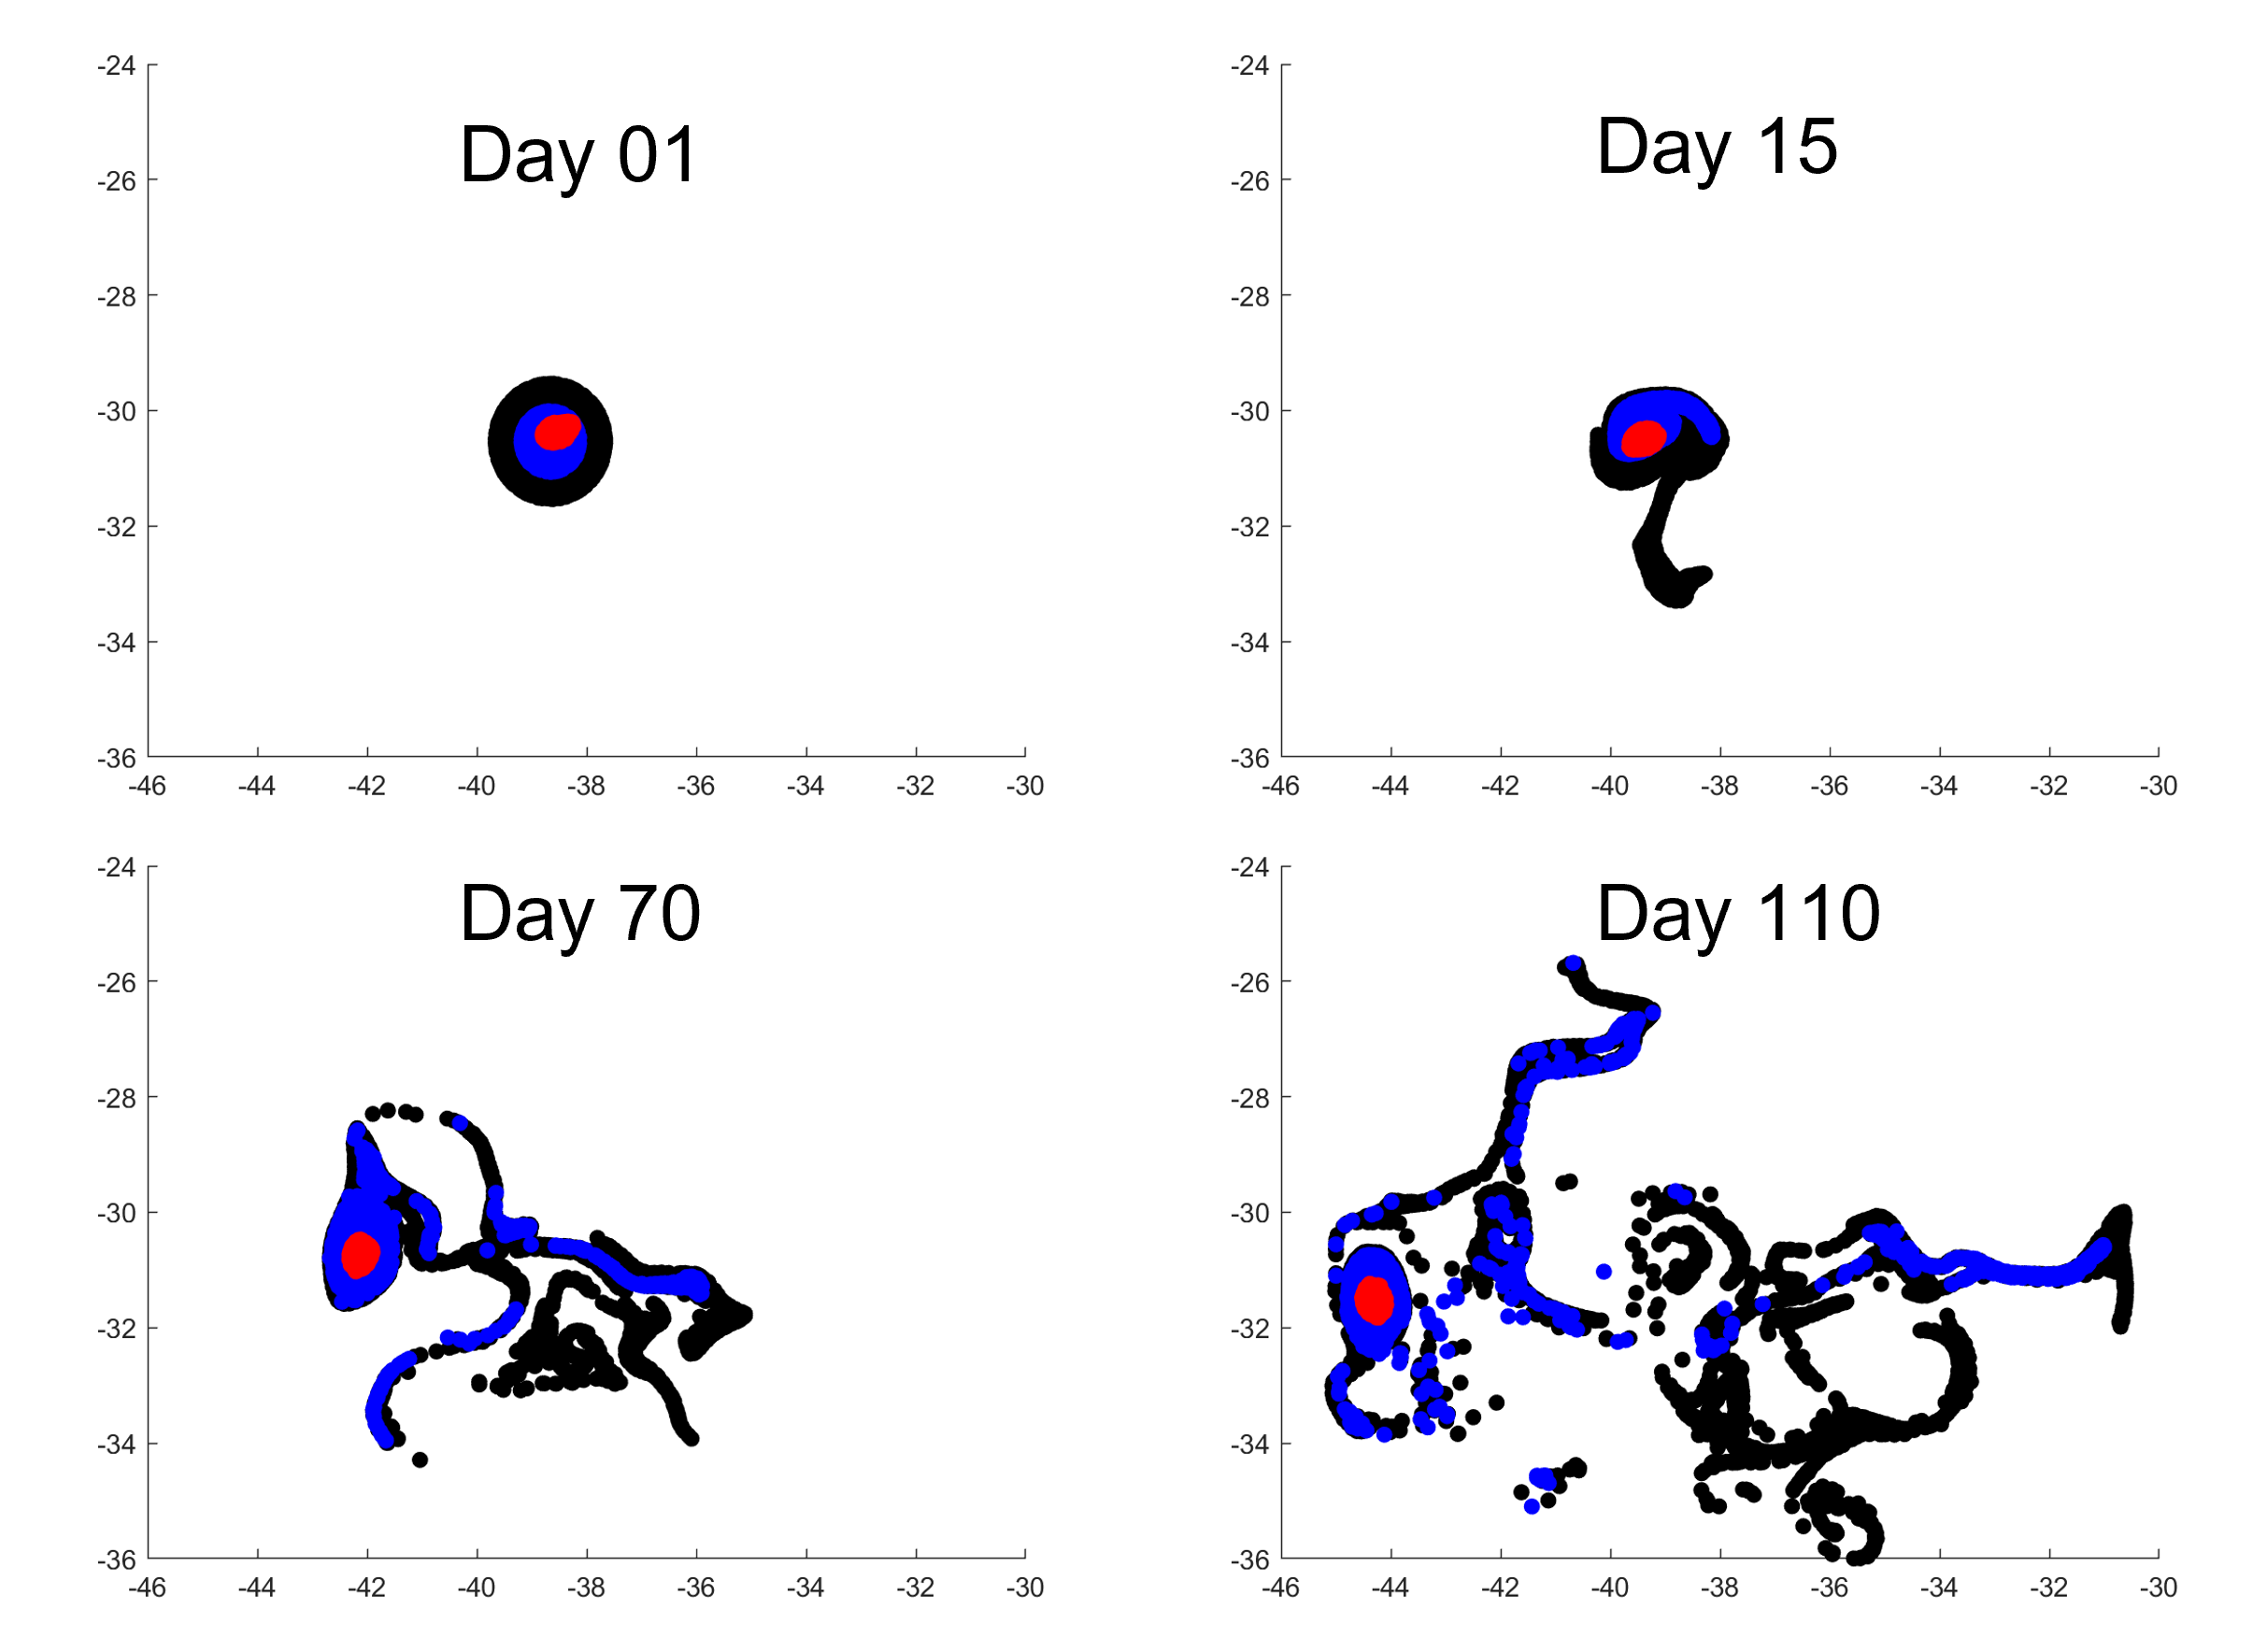
\includegraphics[width=1.0\textwidth]{chapter/figure/coherence of eddy.png}
  \caption
  {Evolution of one elected eddy}
  \label{coherence of eddy}
\end{figure}

Lagrangian eddies-detecting algorithms, thus, provide a convincing path to estimate eddies' number, size and carrying capacity for transporting a large amount of waters and particles both in oceanic model data and observational data.

\clearpage

\section{Conclusion}

In this chapter, we use SSHA Eulerian method to detect eddies in the same research area and research period. We have several findings as concluded below:

\begin{itemize}
  \item [1)] 
  The general appearance rules of the Eulerian eddy are quite the same as the Lagrangian eddy.
  \item [2)]
  Eulerian eddies tend to have a bigger size and the number of eddies counted using the Eulerian method outweighs the number in LAVD research.  

  \item [3)]
  A case study of one long-living eddy suggests the robustness of the Lagrangian coherent eddy's  transport capacity.

  \item[4)]
  30 days may be a reasonable choice for the detection period for oceanic eddy. 
\end{itemize}


\newpage


\chapter{Comparison of different eddy detection methods}\label{sec-eval}

In this chapter, we evaluate the robustness of the Lagrangian method by comparing the eddy detecting results between SSHA Eulerian method (as illustrated in figure \ref{A schematic SSHA anticyclonic eddy}) and the LAVD method.

\section{Introduction of Mesoscale Eddy Trajectory Atlas}

We download \href{https://www.aviso.altimetry.fr/en/data/products/value-added-products/global-mesoscale-eddy-trajectory-product/meta2-0-dt.html}{Eulerian eddies trajectories data}  from AVISO+, which detected eddies from Sea Level Anomaly field of merged altimetry datasets using SSHA method as described in chapter \ref{Eulerian methods} and told us information of type, speed, and radius of Eulerian eddies globally \cite{chelton2011global}. This dataset contains eddies with a life cycle of more than 4 weeks. The time frame of the dataset is from 1993 to the present. In this chapter, all the eddies in the spatial range 70°W to 30°W, 60°S to 30°S are used for the statistical analysis of Eulerian eddies. The time range of the vortex dataset selected for the study is from January 1993 to December 2019.


\section{Statistics results of Eulerian detection method}


The statistics Eulerian detection results are shown below in figure \ref{anticyclonic eddies numbers from 1993 to 2019} and figure \ref{cyclonic eddies numbers from 1993 to 2019} (we separate the research region into $1^\circ \times 1^\circ$ sub-domain and sum up the eddies appearing respectively in each sub-domain). From 1993 to 2019, 13683 eddies were generated in the whole region, 6686 of them are anti-cyclonic eddies and 6997 are cyclonic ones. Among all the eddies, along the coast of South America, only a few eddies were detected, which is consistent with Lagrangian methods. In the northern part and the southwest part of the Argentine Basin, we observe vast numbers of eddies. In the center part of the Argentine Basin, only a few eddies were detected. Many vortices have been observed in the Southern Ocean region or in the connecting water region between Argentine Basin and the Southern Ocean near the islands. The general pattern is quite similar to the results in the chapter \ref{Eddies features analysis} when the Lagrangian method is adopted although the Eulerian method could detect a higher number of eddies.

\begin{figure}[ht]
  \centering
  \setlength{\abovecaptionskip}{0.cm}
  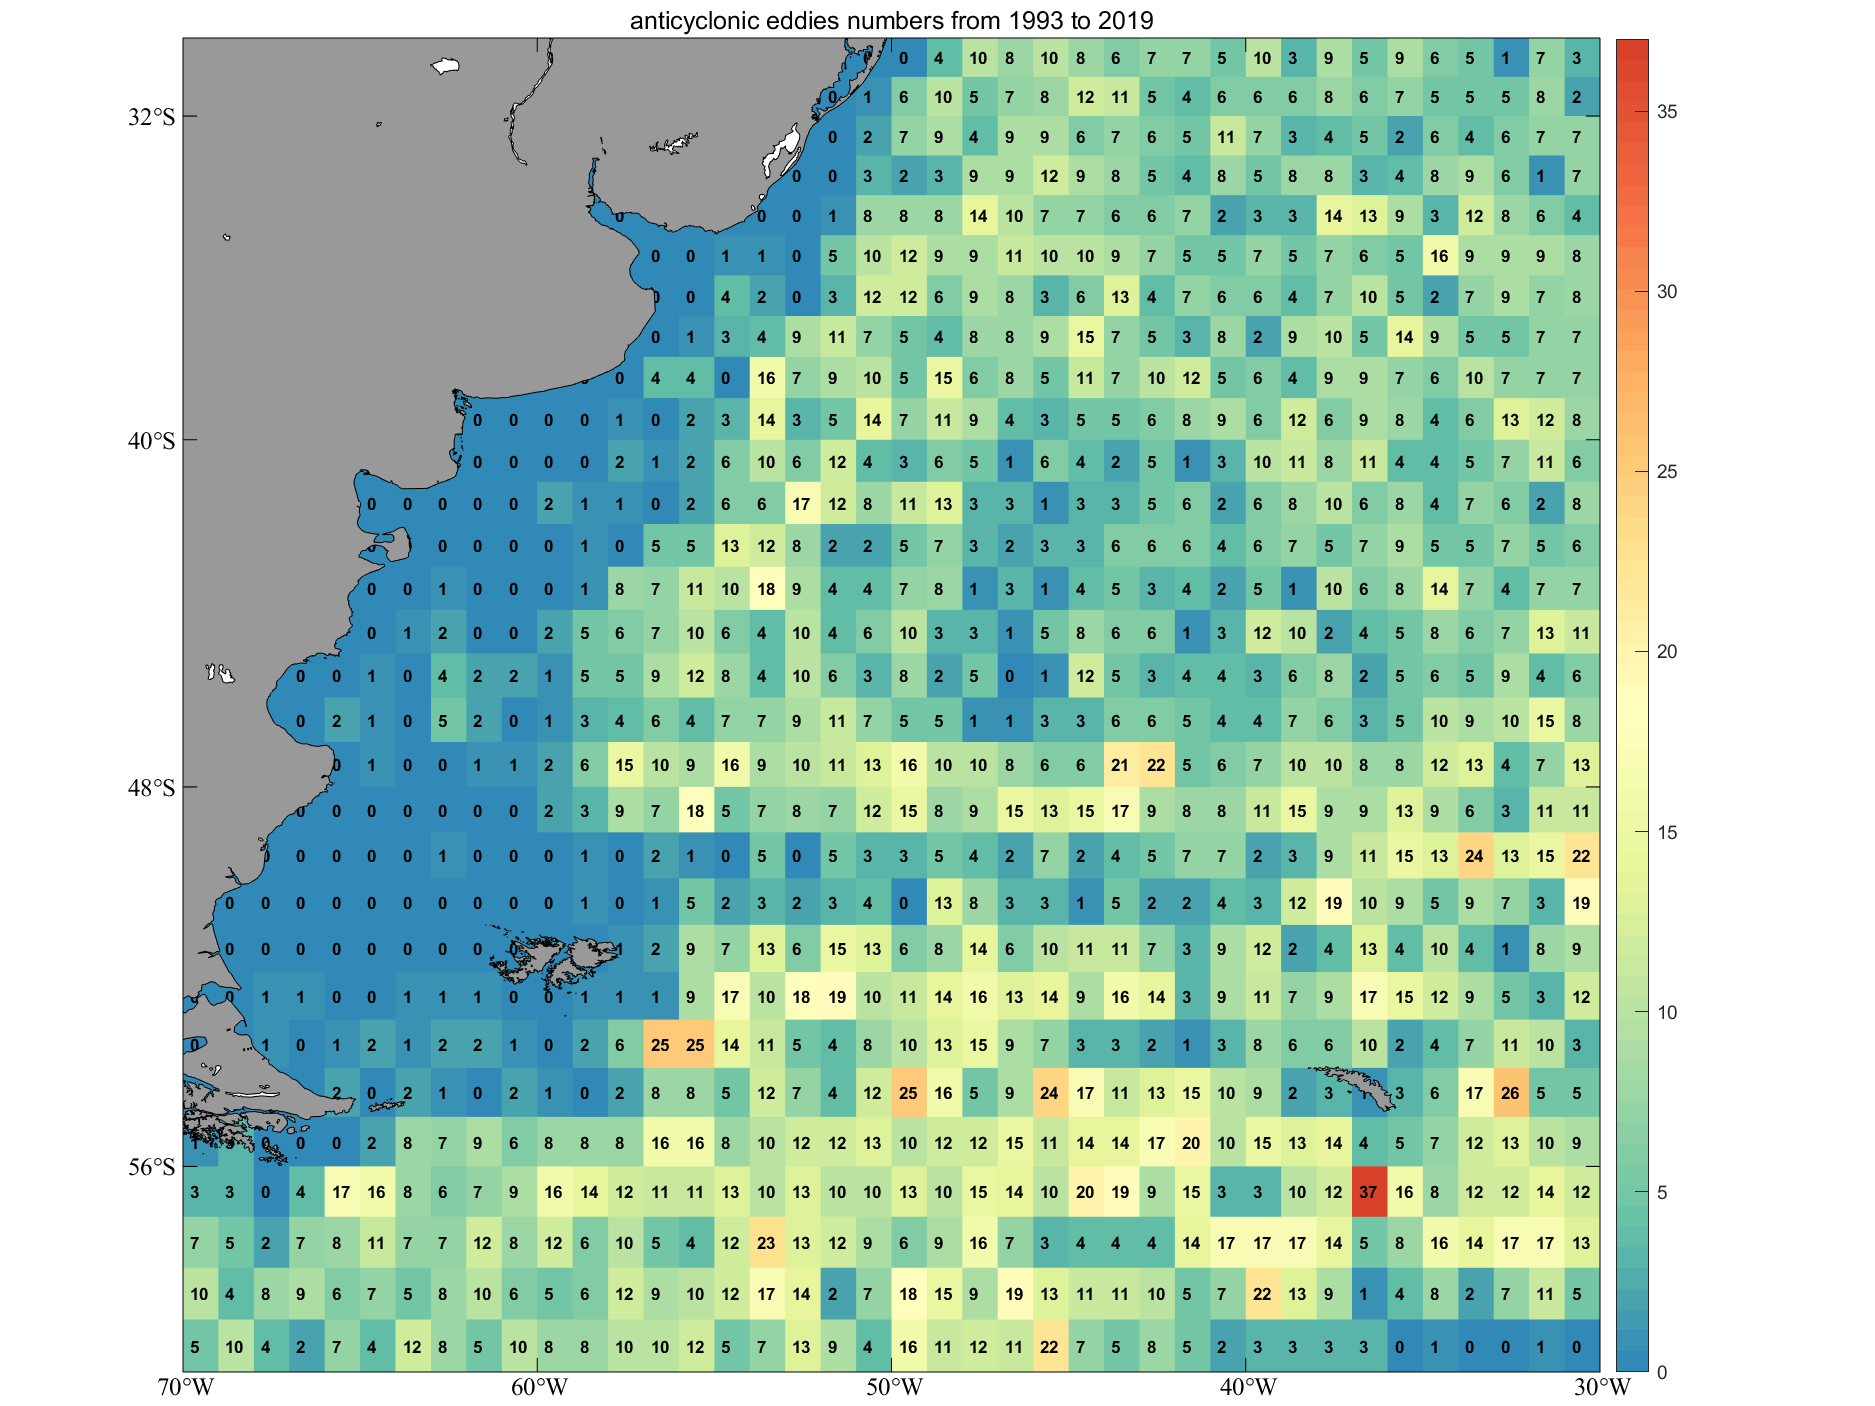
\includegraphics[width=15cm]{chapter/figure/anticyclonic eddies numbers from 1993 to 2019.png}
  \caption
  {Anticyclonic eddies numbers from 1993 to 2019}
  \label{anticyclonic eddies numbers from 1993 to 2019}
\end{figure}

\begin{figure}[ht]
  \centering
  \setlength{\abovecaptionskip}{0.cm}
  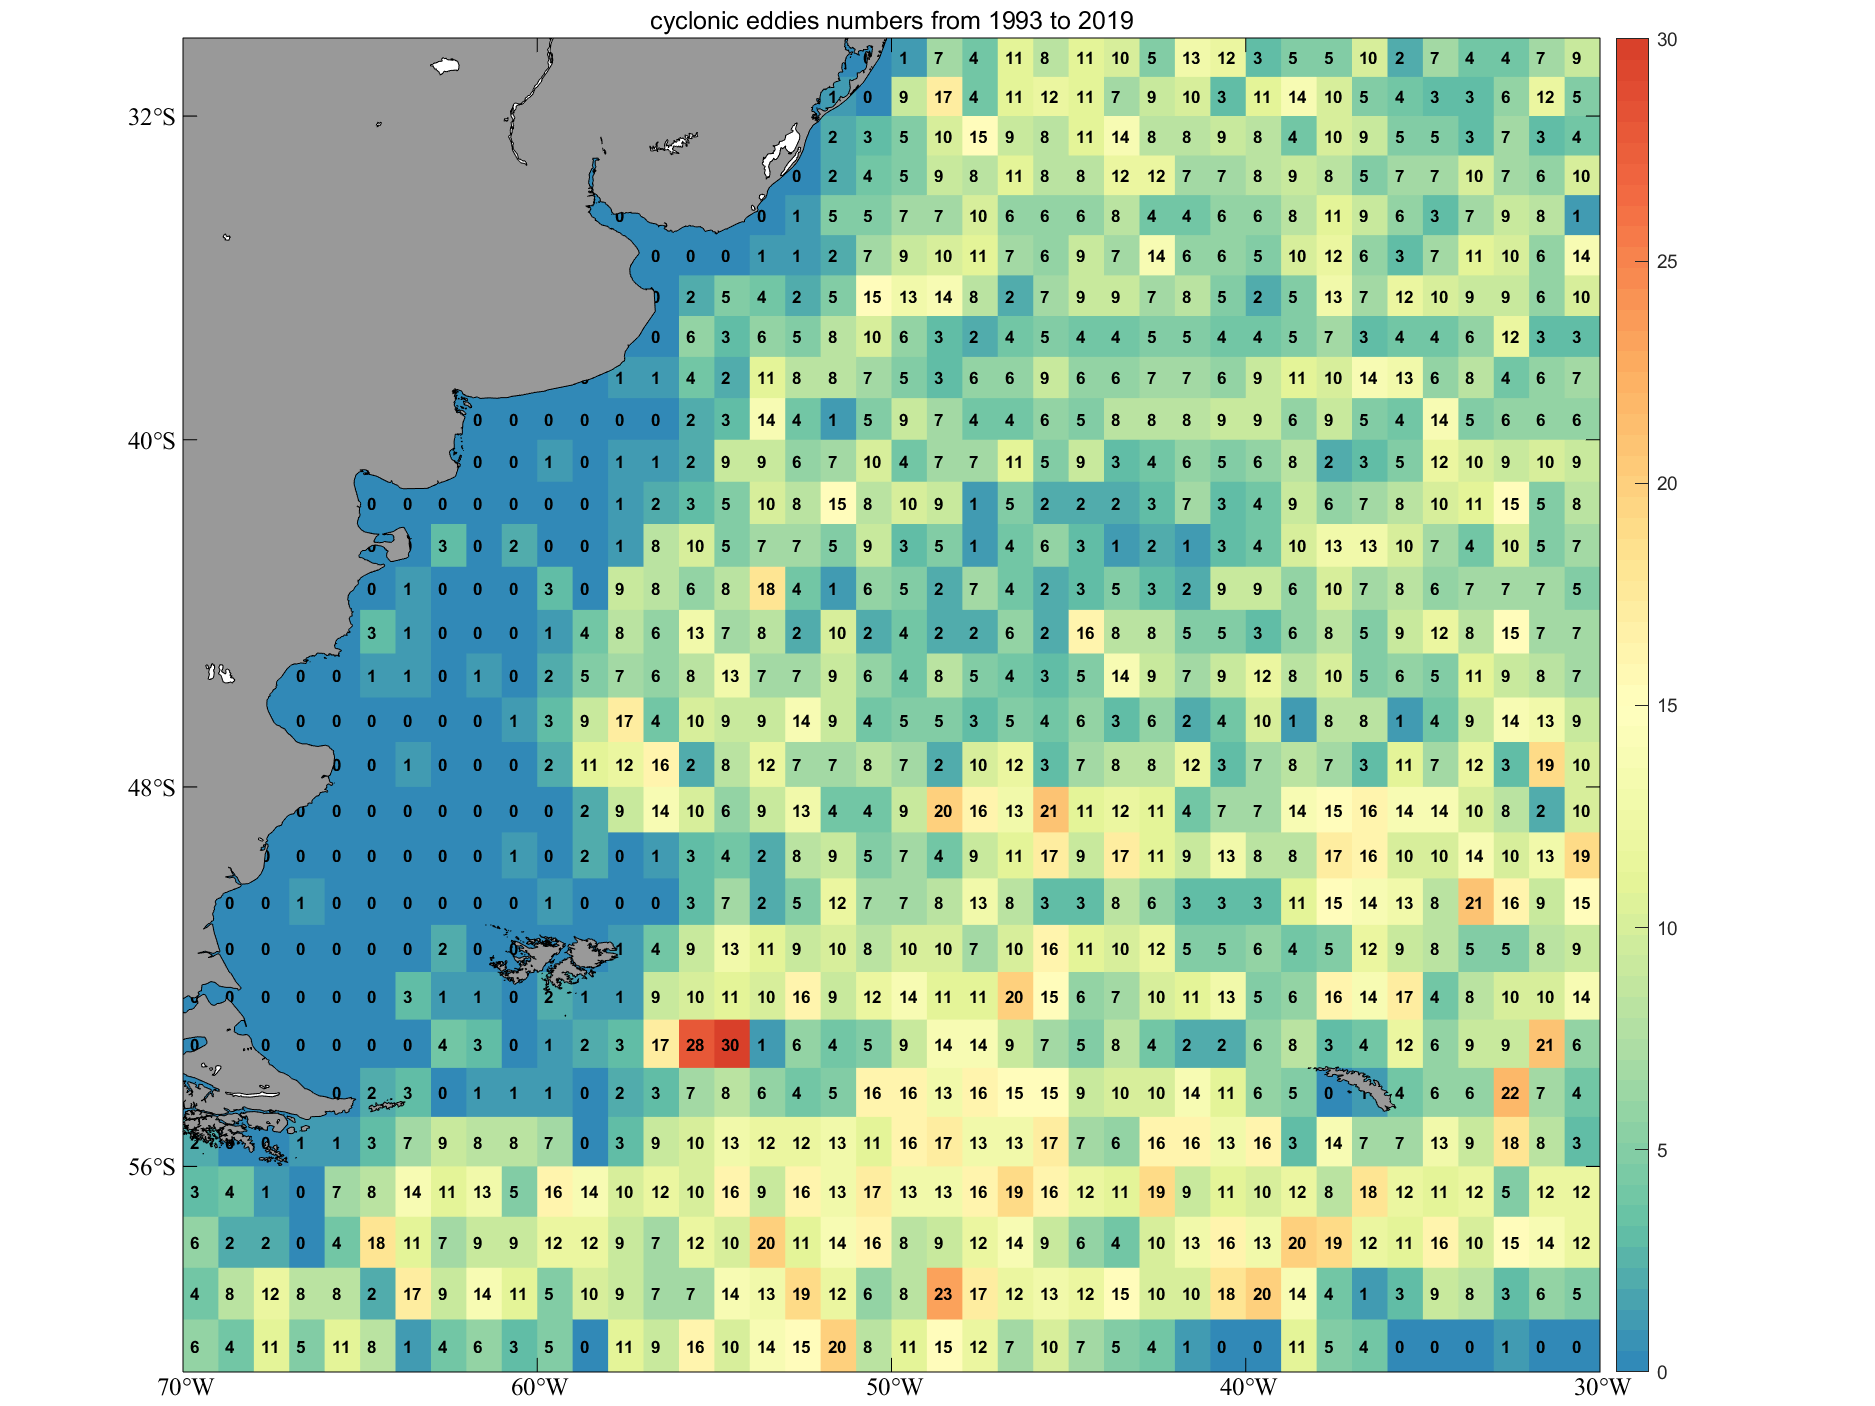
\includegraphics[width=15cm]{chapter/figure/cyclonic eddies numbers from 1993 to 2019.png}
  \caption
  {Cyclonic eddies numbers from 1993 to 2019}
  \label{cyclonic eddies numbers from 1993 to 2019}
\end{figure}

The following figures \ref{Anticyclonic eddies trajectories} and \ref{10 Cyclonic eddies trajectories} are the trajectories map of anticyclonic eddies and cyclonic eddies with lifetimes longer than 30 days. In order not to overlap the trajectories with each other, only one-tenth of the total eddies are selected and plotted on the map.


\begin{figure}[ht]
  \centering
  \setlength{\abovecaptionskip}{0.cm}
  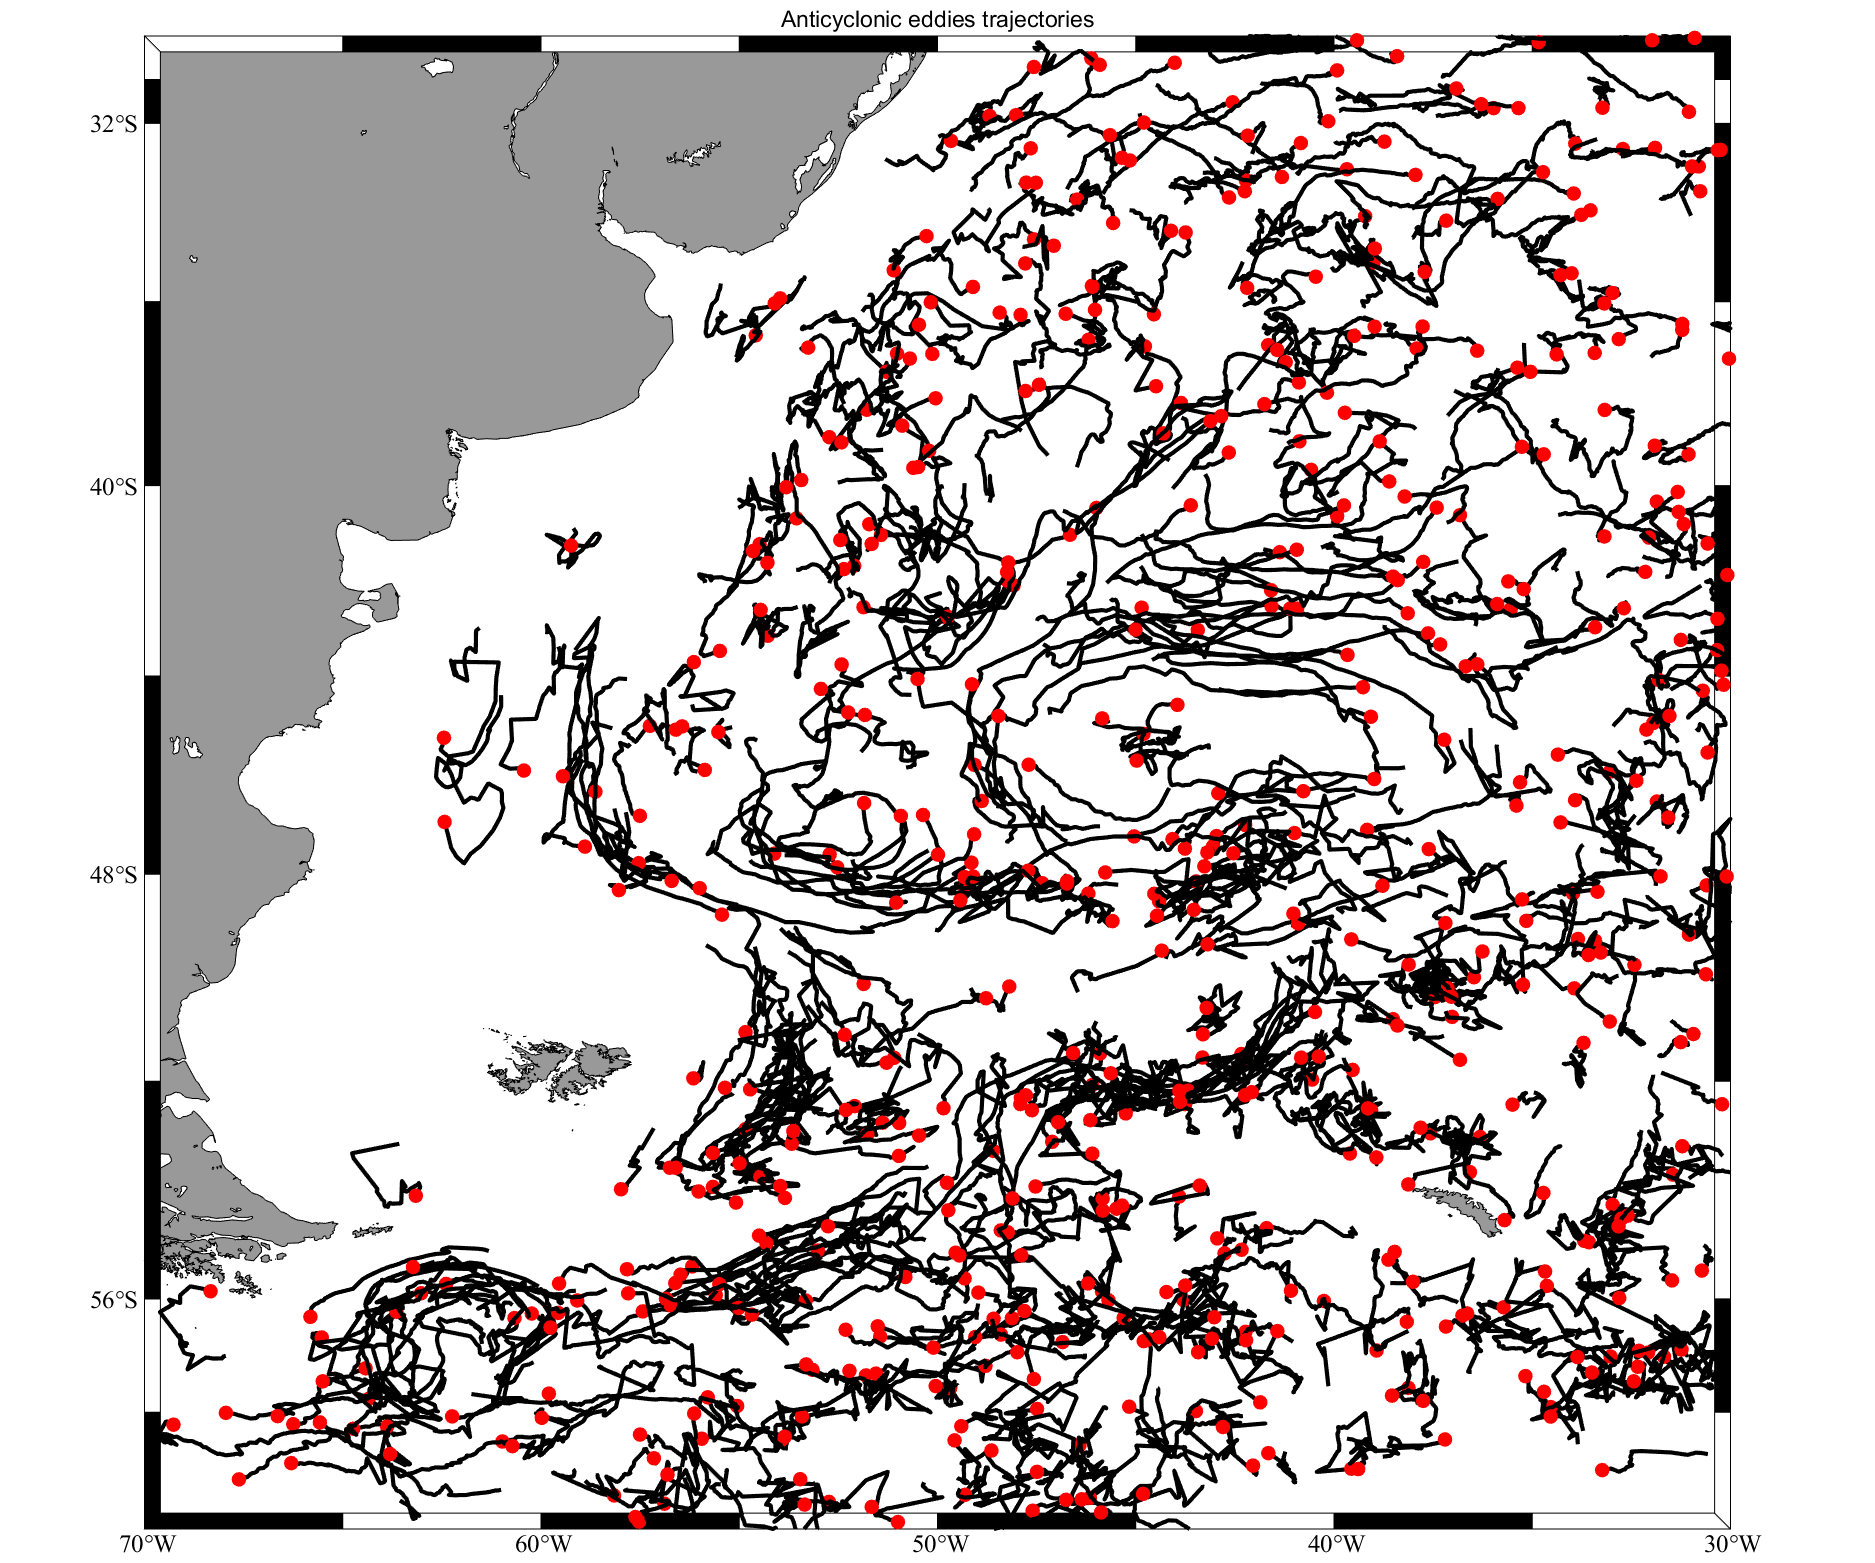
\includegraphics[width=1.0\textwidth]{chapter/figure/10 Anticyclonic eddies trajectories.png}
  \caption
  {Anticyclonic eddies trajectories from 1993-2018}
  \label{Anticyclonic eddies trajectories}
\end{figure}

\begin{figure}[ht]
  \centering
  \setlength{\abovecaptionskip}{0.cm}
  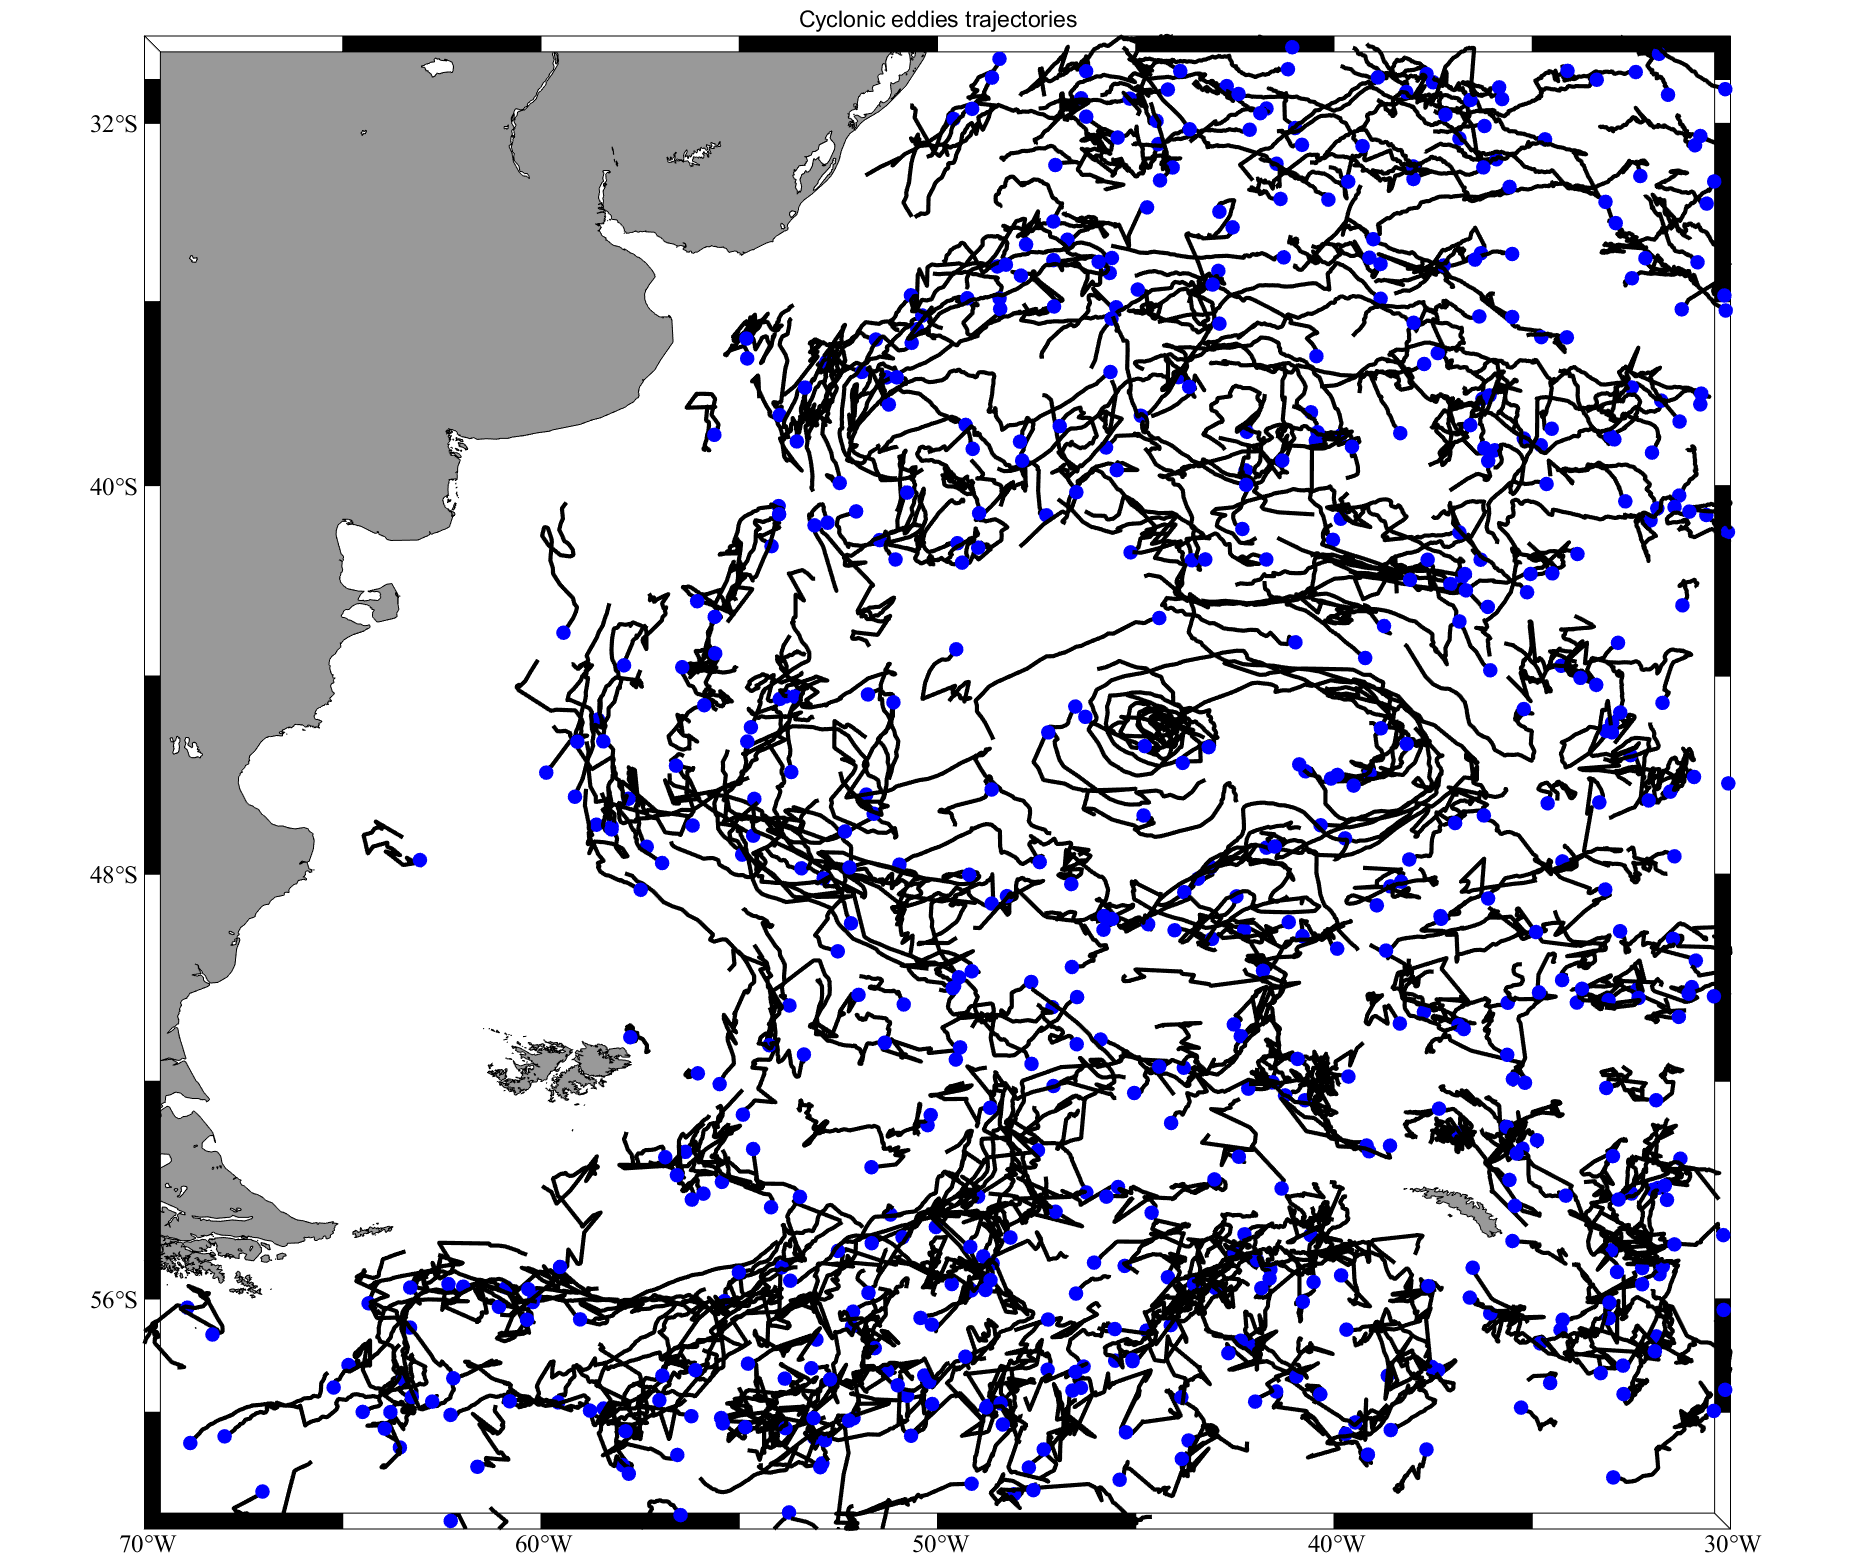
\includegraphics[width=1.0\textwidth]{chapter/figure/10 Cyclonic eddies trajectories.png}
  \caption
  {Cyclonic eddies trajectories from 1993-2018}
  \label{10 Cyclonic eddies trajectories}
\end{figure}


From figure \ref{Eulerian eddy number} , the observed temporal distribution of Eulerian eddies suggests that about 200-300 eddies would be generated in the Argentine Basin each year and the number of eddies decreases a little bit in recent years.
Eddies number distributes unevenly in the four-season: in summer, more eddies would appear and fewer eddies would be generated in winter. This pattern is similar to the results found in chapter \ref{Eddies features analysis}. The number of cyclonic eddies outweighs that of anticyclonic eddies by about 5\%.

The radius of Eulerian eddies is about 70 km, and anticyclonic eddies are a little bigger than cyclonic ones. The result is about twice as large as the Lagrangian eddy, which implies that Eulerian detection method may outweigh coherent transport carried by oceanic eddies and the outer part of Eulerian eddies was not so robust.

\begin{figure}[ht]
  \centering
  \setlength{\abovecaptionskip}{0.cm}
  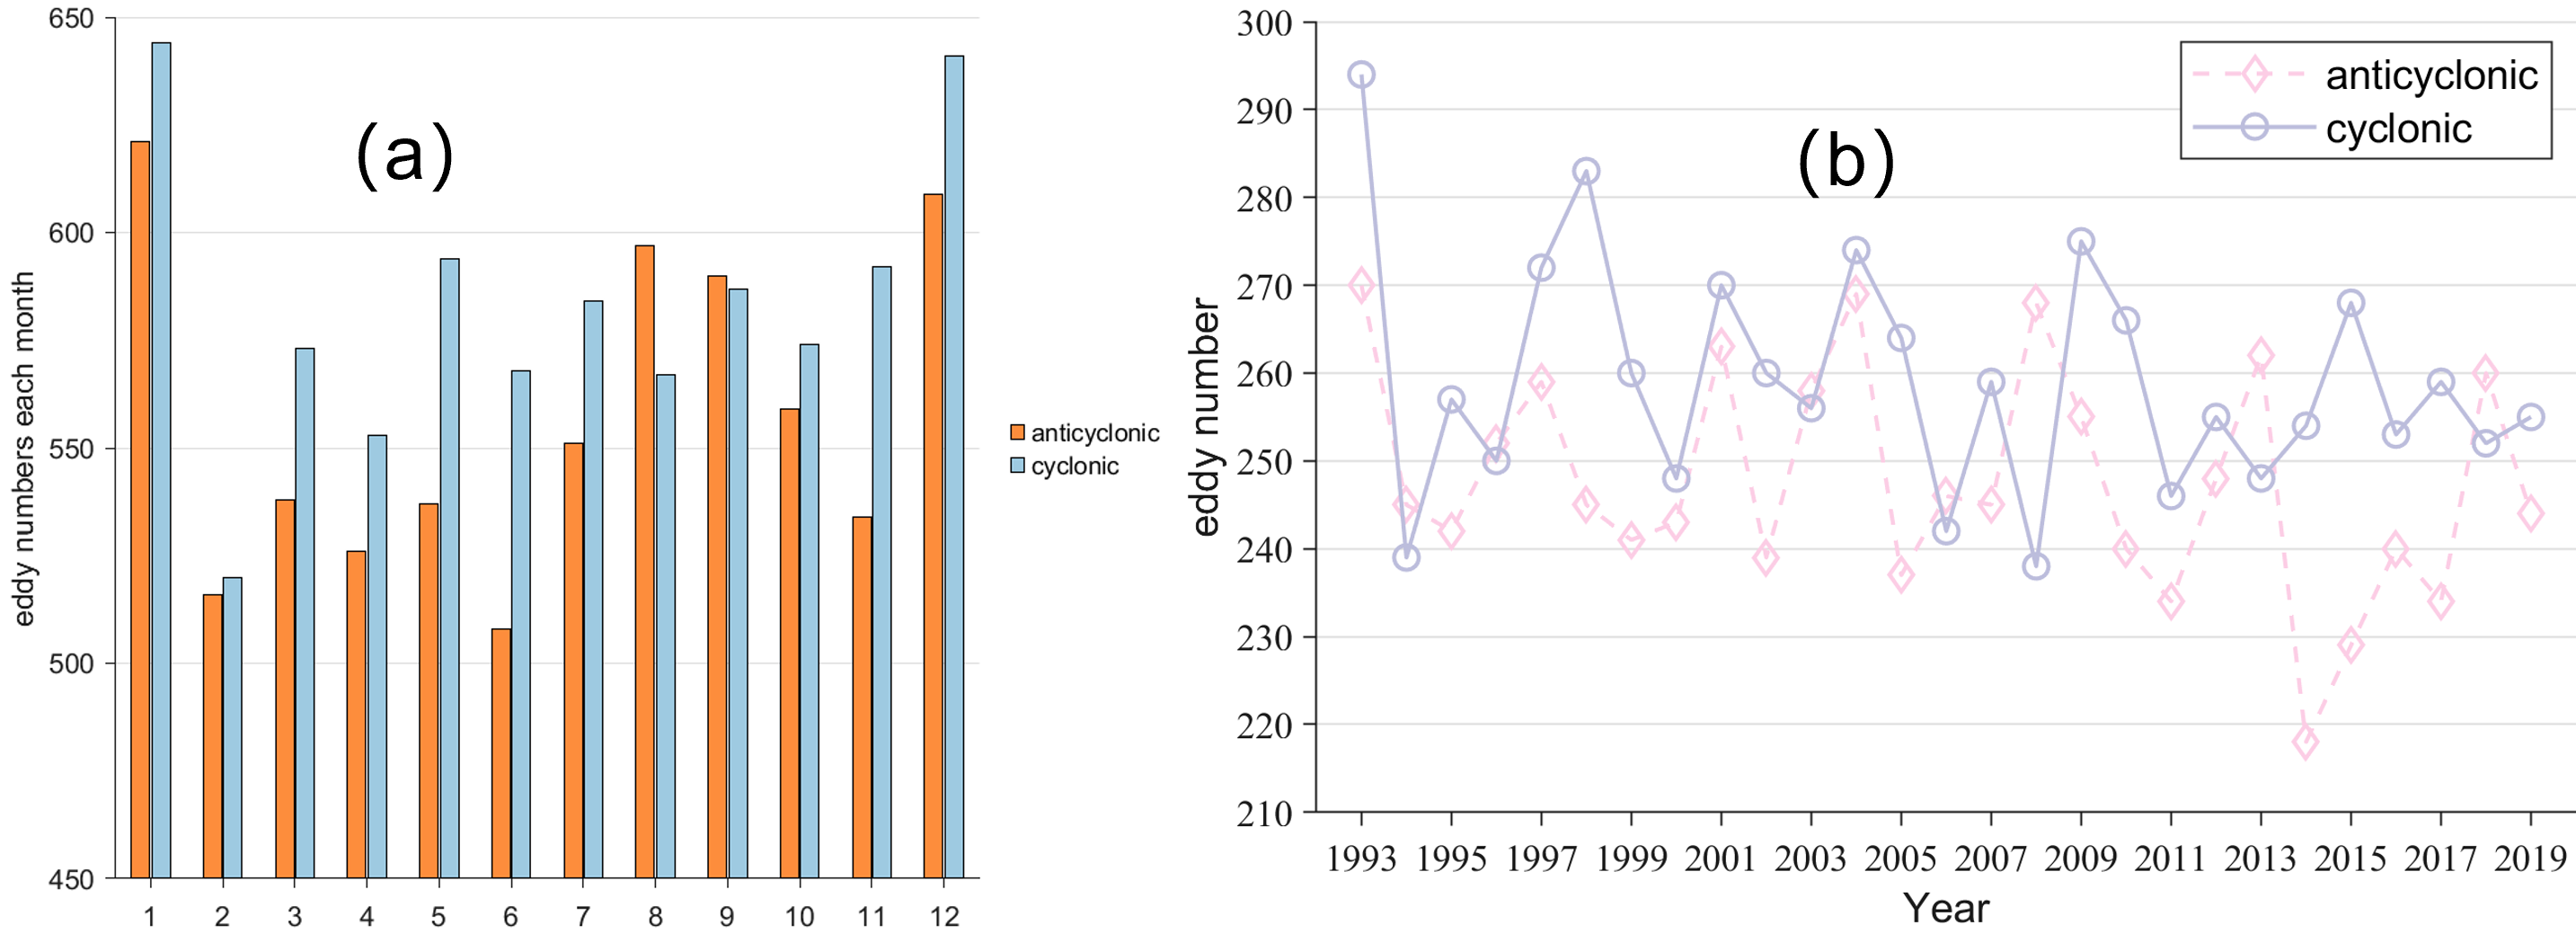
\includegraphics[width=15cm]{chapter/figure/Eulerian eddy number.png}
  \caption
  {Monthly and annual volume change characteristics of Eulerian eddy}
  \label{Eulerian eddy number}
\end{figure}


\begin{figure}[ht]
  \centering
  \setlength{\abovecaptionskip}{0.cm}
  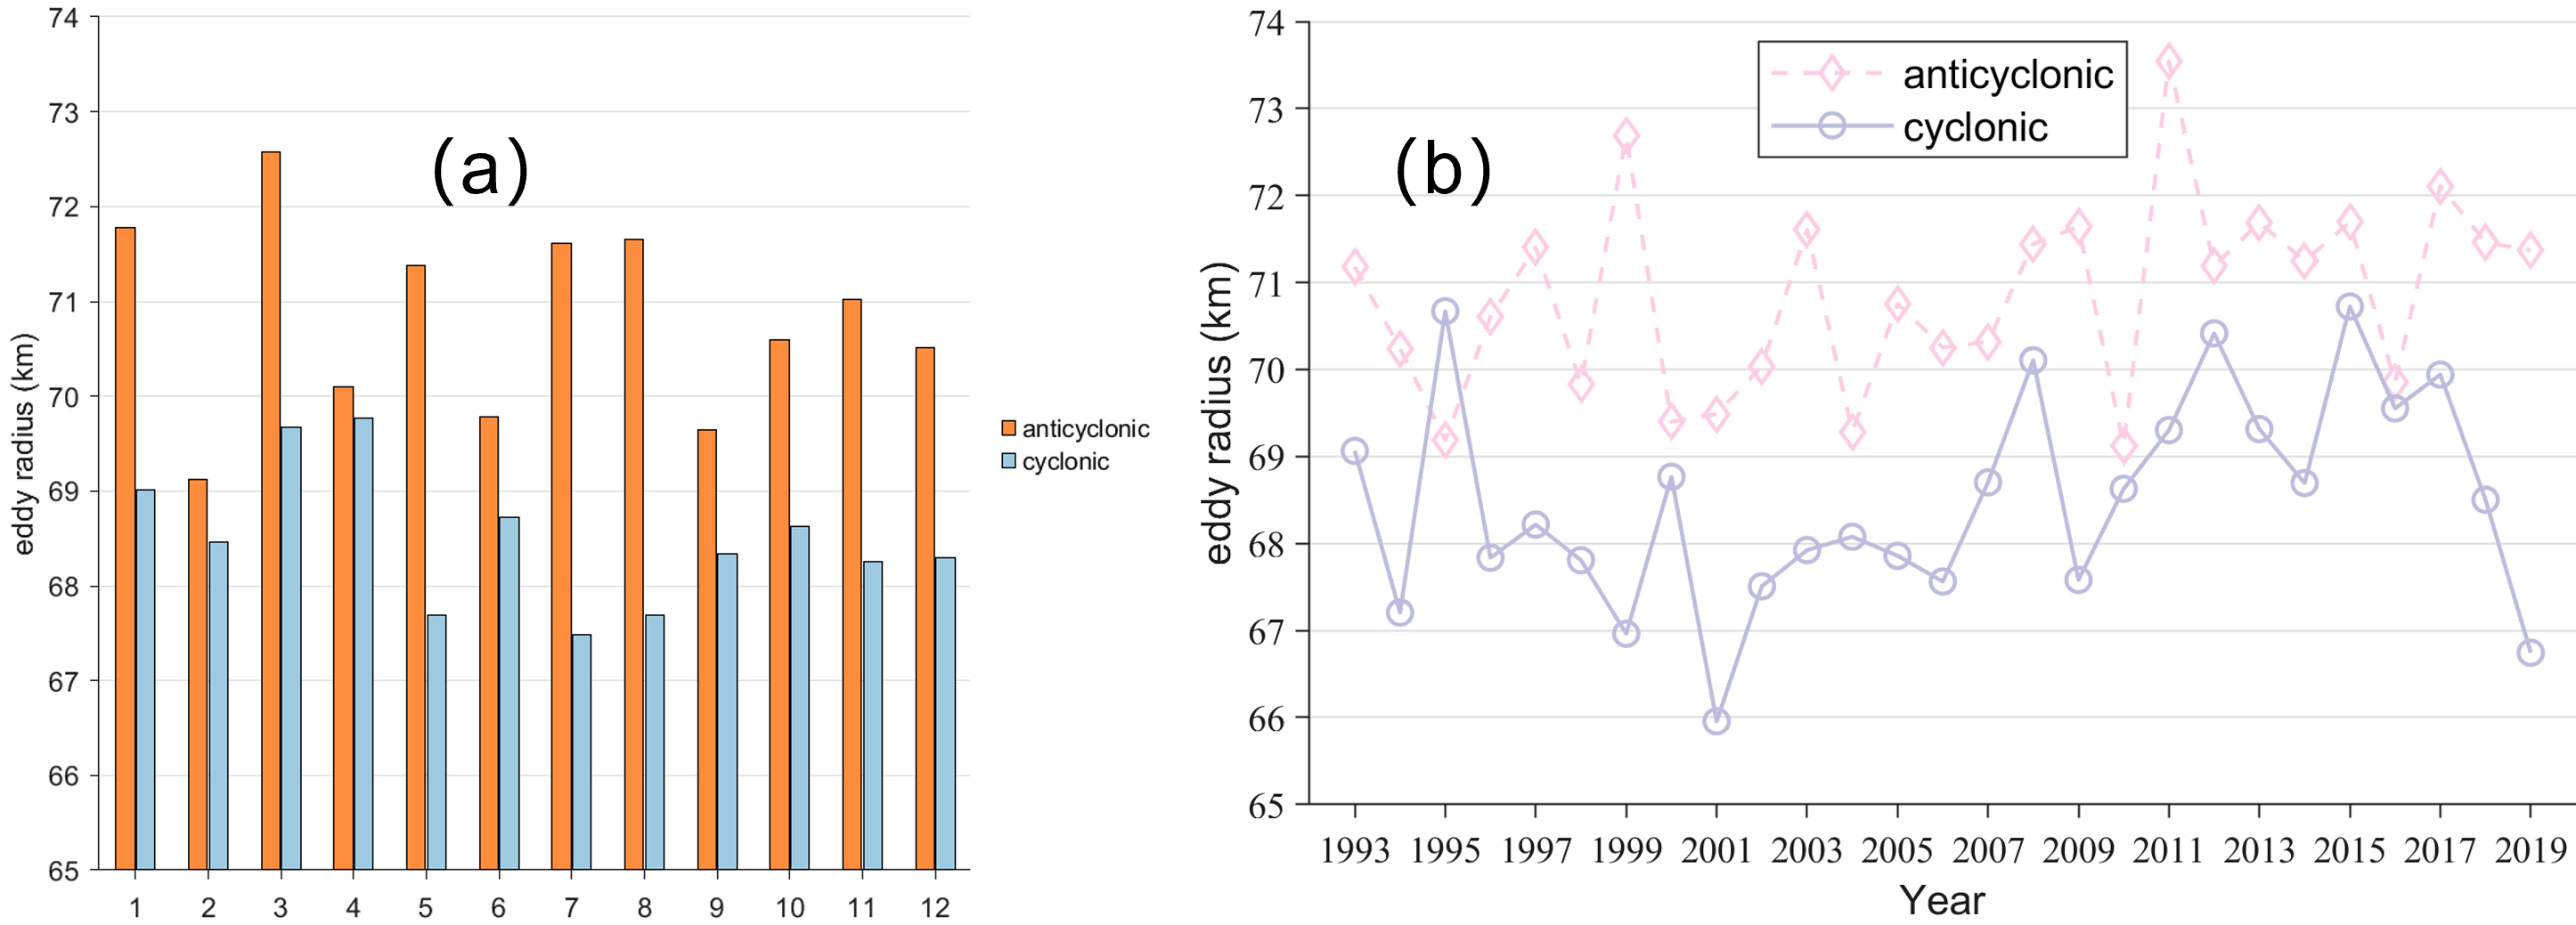
\includegraphics[width=15cm]{chapter/figure/Eulerian eddy radius.png}
  \caption
  {Seasonal and annual variation of Eulerian eddy number and radius}
  \label{Eulerian eddy radius}
\end{figure}


Figure \ref{Cyclonic eddy lifetime Frequency} and \ref{Anticyclonic eddy lifetime Frequency}
show the life estimation of Eulerian eddies, eddies with life estimation ranging from 30 to 60 days occupies 61\% of the entire number of vortexes while eddies with lifetime shorter than 30 days only account for 8\% and eddies with life-range over 180 days only takes up 1.5\% (1.6\% in cyclonic eddies and 1.4\% in anticyclonic eddies). The most long-living eddy lasted for 308 days. Thus, choosing 30 days as the coherent time for LAVD methods is convincing. 

\begin{figure}[ht]
  \centering
  \setlength{\abovecaptionskip}{0.cm}
  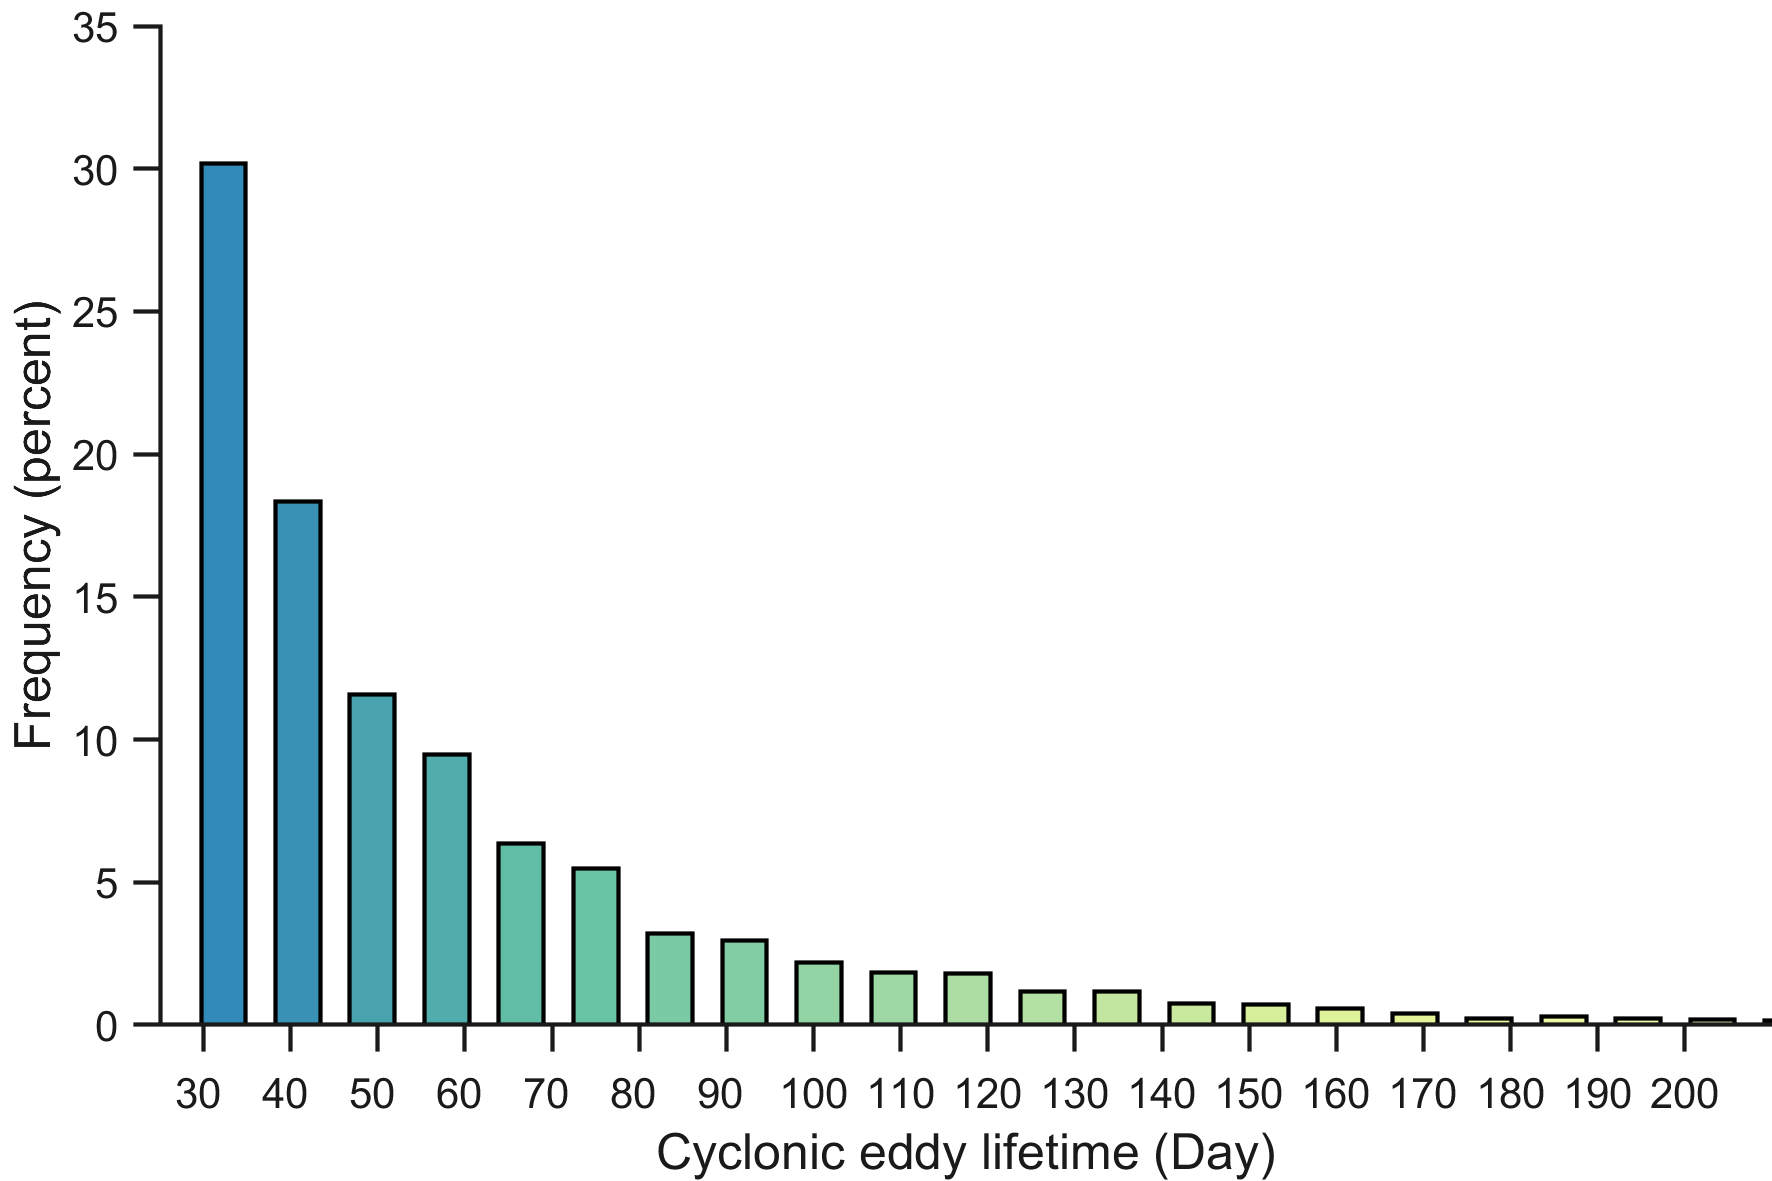
\includegraphics[width=15cm]{chapter/figure/Cyclonic eddy lifetime Frequency.png}
  \caption
  {Cyclonic Eulerian eddy lifetime Frequency}
  \label{Cyclonic eddy lifetime Frequency}
\end{figure}

\begin{figure}[ht]
  \centering
  \setlength{\abovecaptionskip}{0.cm}
  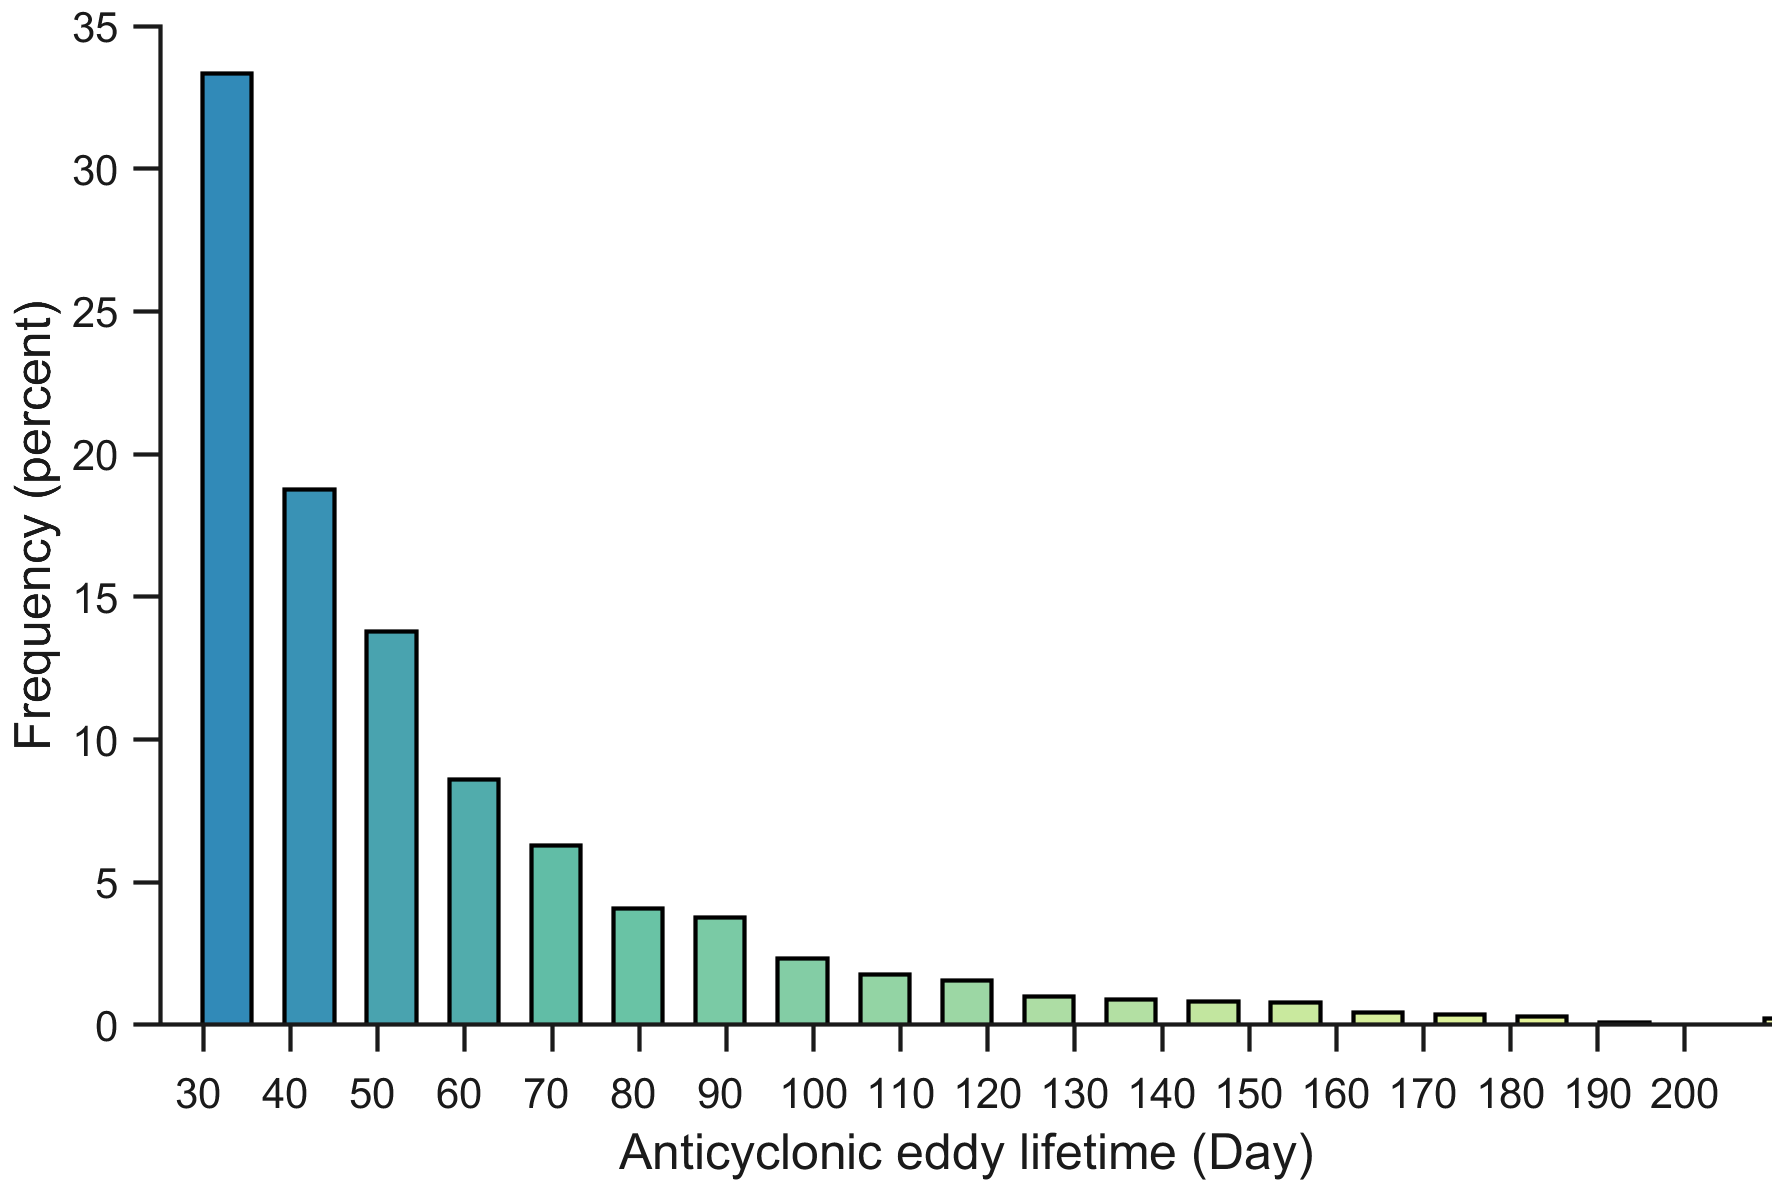
\includegraphics[width=15cm]{chapter/figure/Anticyclonic eddy lifetime Frequency.png}
  \caption
  {Anticyclonic Eulerian eddy lifetime Frequency}
  \label{Anticyclonic eddy lifetime Frequency}
\end{figure}

\section{Comparison of Lagrangian and Eulerian methods}

Since we adopt different methods to detect eddies, it is necessary to test the robustness of the results.


Search through the whole eddies dataset, we have found an Eulerian eddy that originated from 04-Aug-2006 and lasted for 140 days and the corresponding Lagrangian eddy has $t_0 = 2014-09-01$ and a coherent time of 120 days.

Figure \ref{coherence of eddy} shows the evolution process of this selected vortex (x label represents the lontitude and y label represents the latitude). In the figure, the coherent Lagrangian eddy part is marked in red, the blue dots represent the area enclosed by the Eulerian eddy, and the black ring shows the particle outside of the Eulerian eddy. We release the particles and find that the Eulerian eddy could maintain the overall shape in the first 15 days and then the outer part of the Eulerian eddy would deform and stretch in the evolution process. After 70 days, two fluid arms are flung from the core of the Euler vortex and 100 days later, only part of the blue particle is still inside the Eulerian vortex. However, the LAVD Lagrangian eddy still maintains the main body and tracks almost all of the particles inside although the shape of the vortex changes a little bit.

\begin{figure}[ht]
  \centering
  \setlength{\abovecaptionskip}{0.cm}
  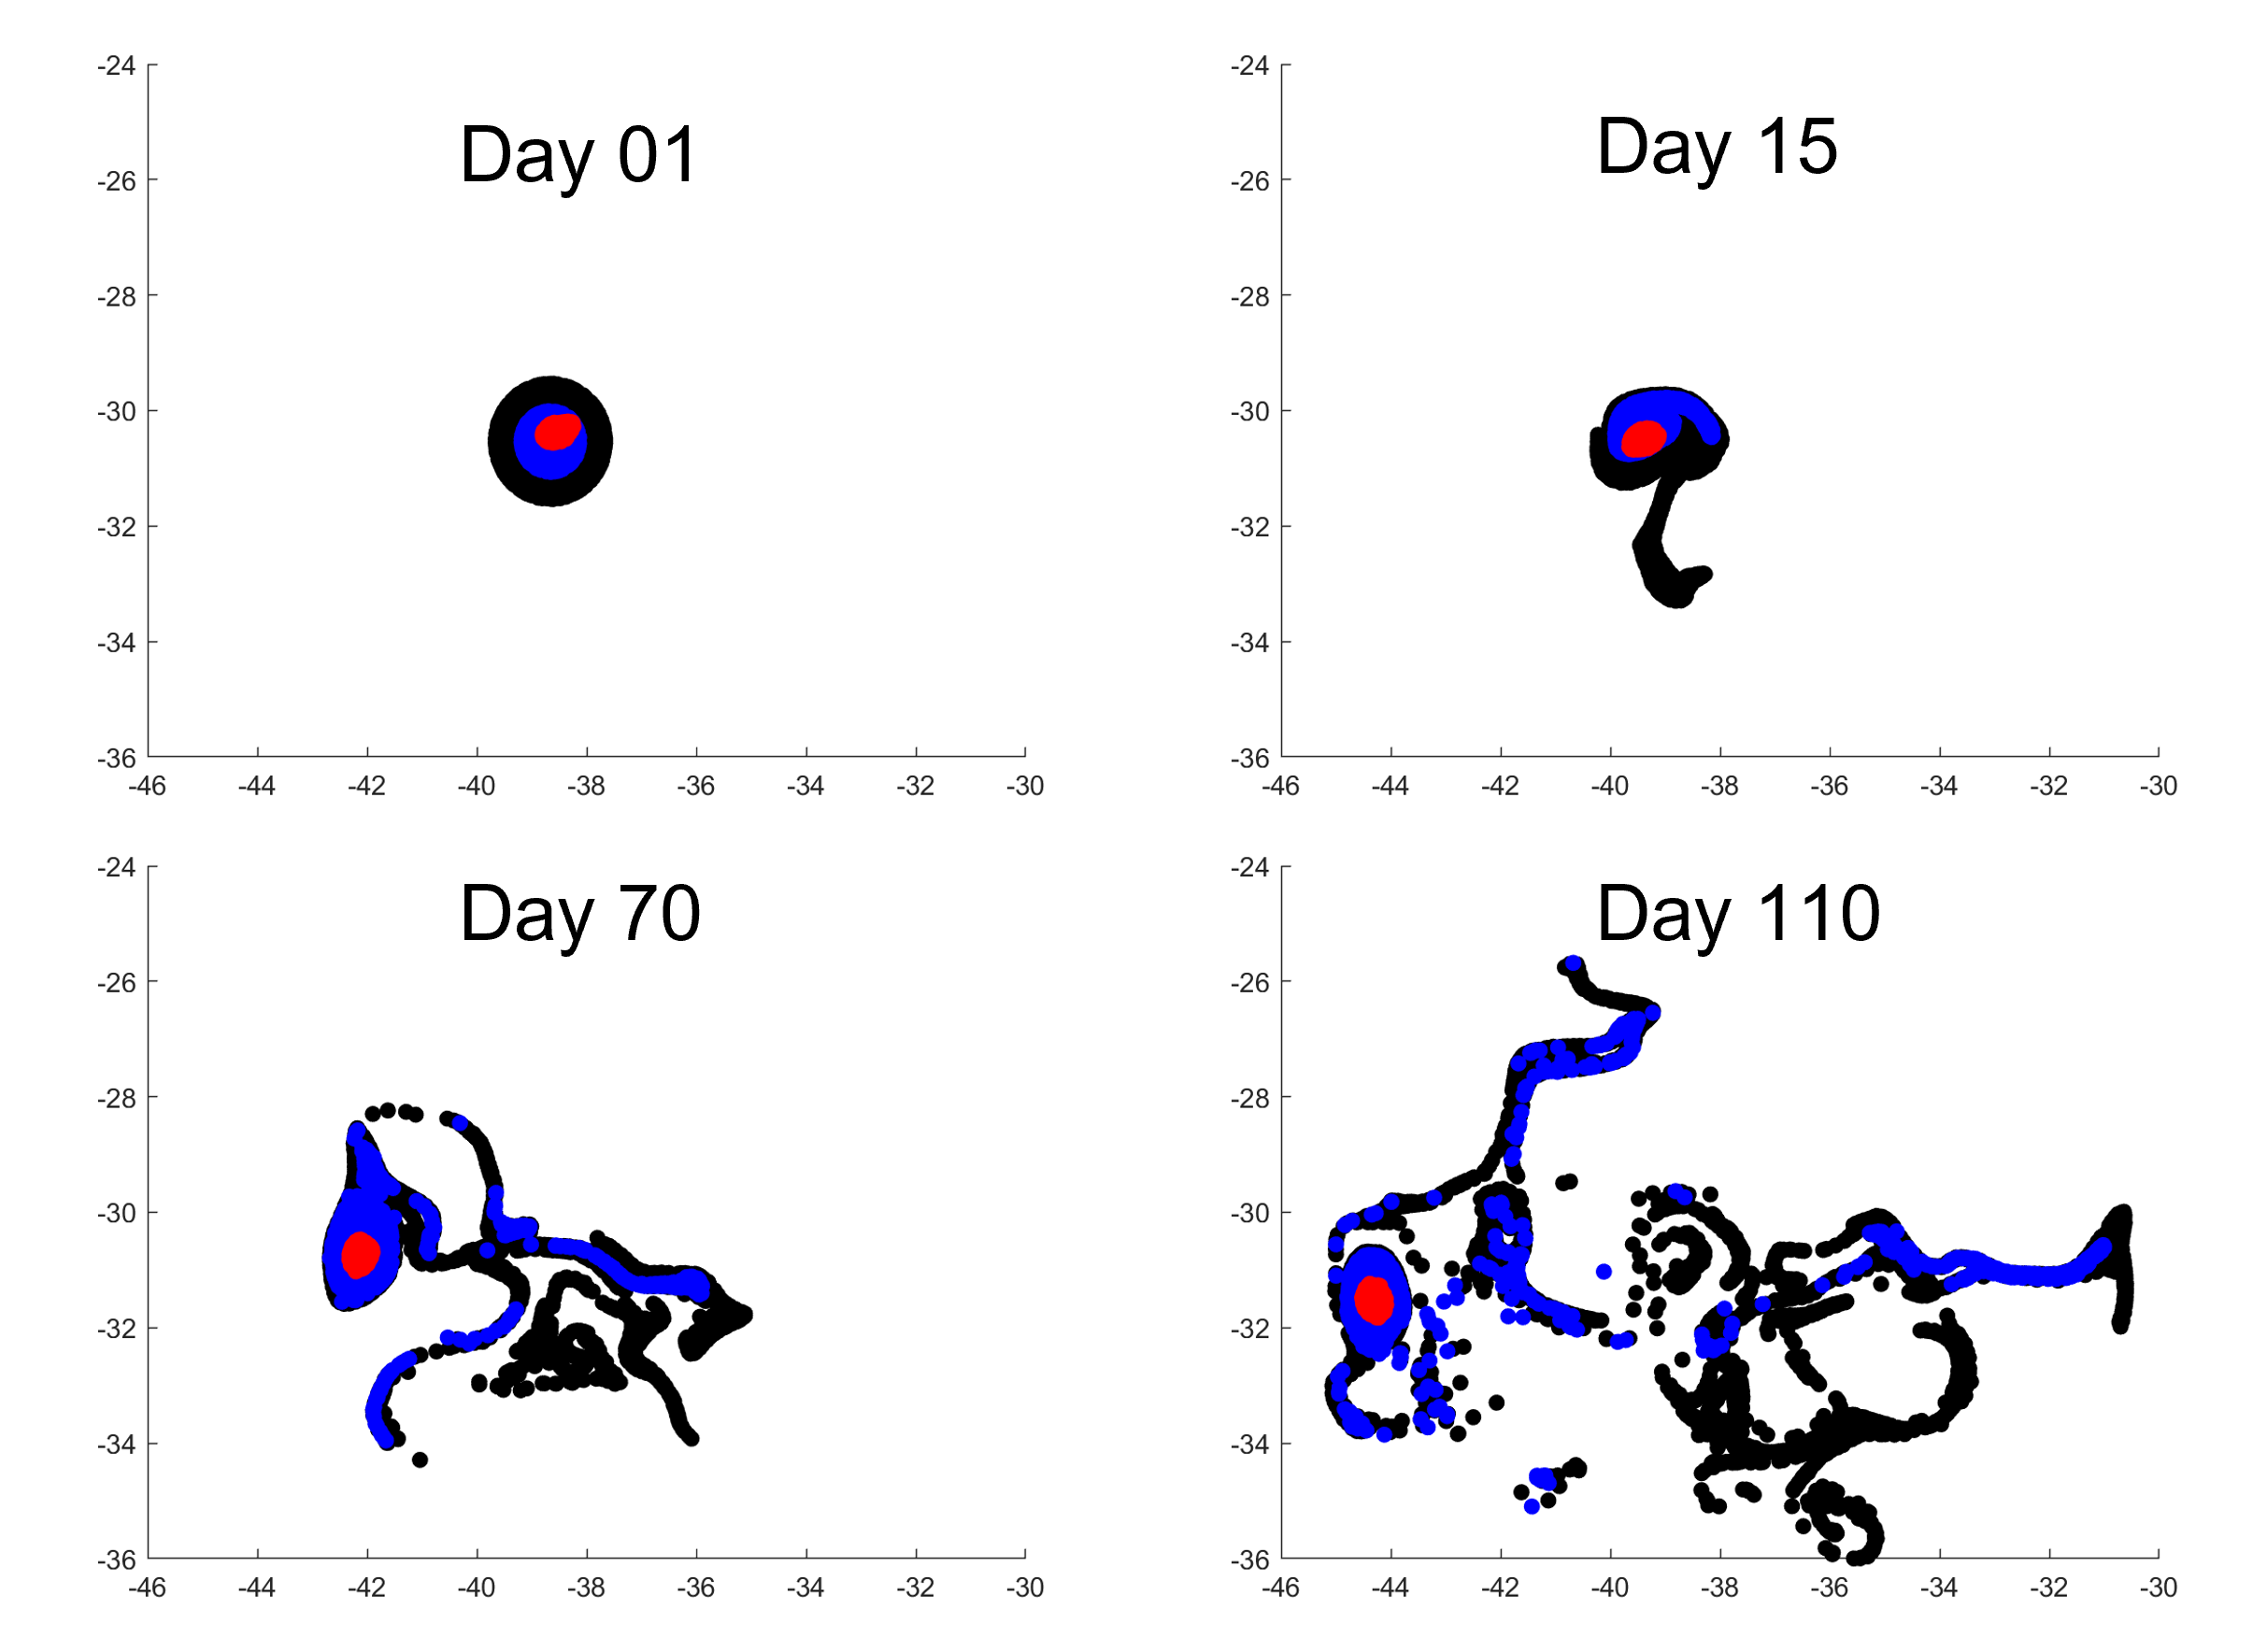
\includegraphics[width=1.0\textwidth]{chapter/figure/coherence of eddy.png}
  \caption
  {Evolution of one elected eddy}
  \label{coherence of eddy}
\end{figure}

Lagrangian eddies-detecting algorithms, thus, provide a convincing path to estimate eddies' number, size and carrying capacity for transporting a large amount of waters and particles both in oceanic model data and observational data.

\clearpage

\section{Conclusion}

In this chapter, we use SSHA Eulerian method to detect eddies in the same research area and research period. We have several findings as concluded below:

\begin{itemize}
  \item [1)] 
  The general appearance rules of the Eulerian eddy are quite the same as the Lagrangian eddy.
  \item [2)]
  Eulerian eddies tend to have a bigger size and the number of eddies counted using the Eulerian method outweighs the number in LAVD research.  

  \item [3)]
  A case study of one long-living eddy suggests the robustness of the Lagrangian coherent eddy's  transport capacity.

  \item[4)]
  30 days may be a reasonable choice for the detection period for oceanic eddy. 
\end{itemize}


\newpage


\chapter{Eddies features analysis} \label{Eddies features analysis}

In this chapter, we present statistical results of coherent Lagrangian eddies using LAVD method.



\section{Eddies statistics}\label{Eddies statistics}

This chapter includes a set of figures showing census statistics about the eddies detected and tracked by applying LAVD method to AVISO dataset. Over the period of 1993-2019, 6212 coherent eddies with radius larger than 20 km and coherence time of 30 days were detected.

The figure \ref{fig:eddy number} shows the monthly and yearly variation patterns of the eddy number. From the figure, we could infer that the number of eddies distributes unevenly in four seasons and shows a trend of increasing from 1993 to 2019. The average number of eddies per month is about 20 and it ranges from 10 to 40. Eddies' number rises to 41, and peaks in December 2014. The months with the fewest eddies were Feb 2000, Apr 2007, Jun 1994, and Oct 2010, and only 10 eddies were detected in those months as shown in section (c) of the figure \ref{fig:eddy number}.  

In December, around 600 eddies were detected from 1993 to 2019 while only 452 eddies were detected in June. Seasonal change of eddy number shows that eddy number peaks in summer, decreases rapidly, and reaches the minimum value in winter. From (b) part of the figure \ref{fig:eddy number}, we could come to a conclusion that eddies number increases over the last three decades, showing a hint of how global warming would increase the instability of the upper ocean and the increasing rate is 3/year.

\begin{figure}
    \centering
    \includegraphics[width = 15cm]{chapter/figure/Eddy number per month and per month.png}
    \caption{Eddy number per month and per month}
    \label{fig:eddy number}
\end{figure}

The average eddy radius is 32.98 km and the standard deviation is 11.31 km. From the eddy radius histogram as shown in section (c) of the figure \ref{Eddy radius map}, we could infer that most of the eddies fall within the range of 20-30 km. The frequency of eddy radius decreases exponentially with increasing radius. From section (b) of the figure \ref{Eddy radius map}, eddy radius does not show an upward or downward trend year by year. Eddies that were generated in 2019 show an average maximum value of 34.41 km while eddies reached the minimum value (31.3 and 31.5 km) in 1996 and 1997. The monthly change of eddy radius shows a minimum value in July and August and a maximum value in December.

Combining the information on eddy number and eddy radius, we may come to the conclusion that in winter, the number and radius of eddies will be reduced due to insufficient energy in the upper ocean.

\begin{figure}
    \centering
    \includegraphics[width =15cm]{chapter/figure/eddy radius2.png}
    \caption{Eddy radius frequency distribution histogram}
    \label{Eddy radius map}
\end{figure}

The figure \ref{radius vs latitude} shows how eddy's radius changes with latitude. From the figure, we could learn that eddies in high latitudes would tend to have a smaller radius, and eddies in lower latitudes would have a larger radius. We also calculated the stretching ratio between the initial eddy area and the final eddy area and the result is shown in figure \ref{enlargement vs latitude}. We infer that eddy would have an inclination to be compressed during the coherent period and the ratio reduces to 0.85 from  $-55^\circ$ S to $-60^\circ $ S, which suggests that the LAVD method may not be so robust in high latitude.

\begin{figure}
    \centering
    \includegraphics[width = 15cm]{chapter/figure/radius vs latitude.png}
    \caption{Relationship of vortex radius with latitude}
    \label{radius vs latitude}
\end{figure}

\begin{figure}
    \centering
    \includegraphics[width = 15cm]{chapter/figure/enlargement vs latitude.png}
    \caption{Relationship of vortex stretching ratio with latitude}
    \label{enlargement vs latitude}
\end{figure}

The figure \ref{velocity vs latitude} demonstrates how eddy propagates in the coherent period. The average propagation speed of the eddy is approximately 5km/day and eddies have the largest propagation speed (about 6.5 km/day) in the middle latitude ranging from $-50^\circ$ S to $-40^\circ$ S. However, the propagation speed will reduce to about 3.6 km/day in higher or lower latitude. There are many outliers for the vortex transport speed in the figure \ref{velocity vs latitude}, which implies the nonlinear effects and causes the vortex moves disorderly. What is more, in most of the cases, the eddy's zonal transport velocity outweighs its meridional component. As shown in figure \ref{Relationship of zonal and meridional velocity with latitude}, the maximum value of zonal velocity is 5.61 km/day near -45°S latitude while the maximum value of meridional velocity is 4.88 km/day at latitudes between -47°S and -50°S. They both show the trend of maximum at intermediate latitudes and decreasing at both low and high latitudes.


\begin{figure}
    \centering
    \includegraphics[width = 1.0\textwidth]{chapter/figure/velocity vs latitude.png}
    \caption{Relationship of eddy velocity (km) with latitude}
    \label{velocity vs latitude}
\end{figure}

\begin{figure}
    \centering
    \includegraphics[width = 15cm]{chapter/figure/eddy velocity vs latitude.png}
    \caption{Relationship of zonal and meridional velocity with latitude}
    \label{Relationship of zonal and meridional velocity with latitude}
\end{figure}

The geographical distribution of eddies from 1993 to 2019 is given in the figure \ref{Eddy polarity map}. Among the 6212 vortices, 3336 of them are cyclonic eddies while 2876 of them are anti-cyclonic, which means that cyclonic vortices outweigh anticyclonic ones by about $15\%$. Along the southwest edge of the Argentine Basin, the majority of eddies were cyclonic eddies. Eddies distribute evenly in the Southern Ocean region, while there are more eddies in the northeast part of the Argentine Basin. There is a vortex "vacuum" zone in the center of the Argentine Basin, with only a few vortices remaining there. In the shallow water areas near South America Continent, we detected more anticyclonic vortices. There are few eddies detected in the coastal region since the deviation of altimeter data near the coastline is rather high due to the influence of tides and coastal waves. In the water regions connecting the Southern Ocean and Argentine Basin, eddies distribute in a striped pattern.

\begin{figure}
    \centering
    \includegraphics[width = 15cm]{chapter/figure/eddy polarity map.png}
    \caption{Eddy polarity distribution map}
    \label{Eddy polarity map}
\end{figure}

The figure \ref{eddy number vs Polarity} shows annual variation and monthly variation of eddy number and vortex radius of cyclonic and anti-cyclonic eddies. Anti-cyclonic eddies have distinct seasonal variations while seasonal number differences of cyclonic eddies are small. In all months, the number of cyclonic vortices is higher than the anti-cyclonic ones. The average number of anti-cyclonic eddies appearing in June is 7.59, which is the lowest in all months. Anti-cyclonic eddy number reaches the minimum value in winter and it increases slowly and reaches a maximum in winter. Annual variation characteristics of vortex numbers tell us that in most of the years, cyclonic eddy numbers outweigh anti-cyclonic ones while the opposite rule was observed in 1995 and 1996. An average of 124 cyclonic vortices and 107 anti-cyclonic eddies are generated each year. Both the number of cyclonic eddies and anti-cyclonic eddies would increase, and the increasing trend of cyclonic eddies is more obvious. The maximum number of annual cyclonic eddies found in the Argentine Basin is 168 in 2019 while the maximum number of annual anti-cyclonic eddies is 133 in 2006.

\begin{figure}
    \centering
    \includegraphics[width = 15cm]{chapter/figure/eddy number vs Polarity.png}
    \caption{Monthly and annual patterns of eddy number of different polarities}
    \label{eddy number vs Polarity}
\end{figure}

Figure \ref{eddy radius vs type} shows how vortex polarity affects vortex size. Before 2010, the diameter of the anticyclonic vortex was more extensive than that of the cyclonic vortex. Since 2007, the radius of cyclonic vortex began to grow and has become bigger than anti-cyclonic ones. From the figure, we could learn that different types of eddies have different seasonal patterns. The average monthly minimum radius of cyclonic eddies is 31.52 km in September while the minimum monthly radius of anti-cyclonic vortices is about 32 km in June. They both show maximum value in December.

\begin{figure}
    \centering
    \includegraphics[width = 15cm]{chapter/figure/eddy radius vs type.png}
    \caption{Monthly and annual patterns of eddy radius of different polarities}
    \label{eddy radius vs type}
\end{figure}

In Figure \ref{eddy classification map_SNWE2}, we compared eddies' initial position and final position from 1993 to 2019 and the figure shows the direction of eddy propagation. About $59\%$ of the eddies would travel northward, and only $41\%$ would travel southward. Anticyclonic vortices are more inclined to transport to the poles. In the east-west direction, about $63\%$ of the eddies travel westward, and only $37\%$ of them travel to the east.

From the map, we could learn that even in the northern part of the Argentine Basin which is affected by the southward Brazil Current, most of the eddies would tend to travel northward, which suggests an opposite direction of the mean flow and eddy flow. Along the border connecting the shallow water region and Argentine Basin, we could learn that eddies in the northern part of the border have an inclination to travel southward and eddies in the southern part have a trend to travel northward. This is coincident with the southward Brazil Current and northward Malvinas Current. In the middle of the Argentine Basin, eddies' travel pattern agrees with the Zapiola Anticyclone.

In the Southern Ocean region, most of the observed eddies travel eastward because of the Antarctic Circumpolar Current. On the northern part of the Argentine Basin, the majority of the eddies propagate westward.
In the center of the basin, because of the Argentine Gyre and branch of the Brazil Current, we could see that at the southern edge of the basin, eddies would tend to move eastward while eddies would move to the west in the middle of the basin.

\begin{figure}
    \centering
    \includegraphics[width = 15cm]{chapter/figure/eddy classification map_SNWE2.png}
    \caption{Eddy travel direction map}
    \label{eddy classification map_SNWE2}
\end{figure}

Figure \ref{some vortex examples} shows some cases study of the  eddies transport path. As shown in section (a) of figure \ref{some vortex examples}, a cyclonic eddy propagates westward in the center of the Argentine Basin. Section b shows an anti-cyclonic eddy on the southern border of the basin and its travel direction is to the southeast. In Section C of the figure, one cyclonic eddy near South Georgia and the South Sandwich Islands goes north and it lost its coherence strongly during the last ten days of transport. Section d of the figure depicts a typical vortex going southward along the South American continental slope, the direction of which is the same as the mean flow thus, a considerable number of vortices are also transported this way.


\begin{figure}
    \centering
    \includegraphics[width = 0.9\textwidth]{chapter/figure/eddy map.png}
    \caption{Some vortex examples (orange for cyclonic eddy and blue for anti-cyclonic eddy)}
    \label{some vortex examples}
\end{figure}

% \section{Eddies morphology}

\section{Eddies coherence time}

In Chapter \ref{Eddies statistics}, we set the coherent time of 30-day and detect 6212 coherent eddies in the study period from 1993 to 2019. However, the properties of the coherent eddy are affected by the selection of time interval to a large extent \cite{xia2022global,vortmeyer2016detecting}.

In the context of the Eulerian detection method (SSHA), the vortex life cycle is defined as the time period of the process of a vortex from birth to death \cite{mccoy2020global,andrade2020genesis}.
According to the previous research, the life cycle of a vortex varies from 4 weeks to  16 weeks and the average life cycle is about 8-9 weeks.

The result is shown in figure \ref{eddy coherent}. From the figure, we could learn that there is a rapid decrease in eddy number when the coherent period is less than 90 days, but the trend slows down after 90 days, which means that an eddy with a life cycle larger than 90 days would tend to survive longer. We could also conclude that eddies with a coherent period of 90 days have the largest radius which suggests that an eddy with a larger radius, magnitude, and intensity will survive longer. 60-day eddies' radius is smaller than 30-day eddies' and 120-day eddies' radius is smaller than 60-day eddies', which 
shows that the time period has an impact on vortex coherence and if we track the eddy exceeding the period $\Delta t$, the outer part of the eddies would be deformed, stretched into filaments, and finally lose coherence.

From figure \ref{eddy type proportion}, we could learn that anticyclonic eddies tend to have larger coherent time. When the coherence period is 30-day, anti-cyclonic eddies only occupy $46\%$ of the total eddy number; while the proportion raise up to $64\%$ when the coherent interval is 120-day.

\begin{figure}[htbp]
    \centering
    \includegraphics[width = 15cm]{chapter/figure/eddy coherent.png}
    \caption{Eddy properties and their relationship with coherence time}
    \label{eddy coherent}
\end{figure}

\begin{figure}[htbp]
    \centering
    \includegraphics[width = 15cm]{chapter/figure/eddy type proportion.png}
    \caption{Eddy type proportion map}
    \label{eddy type proportion}
\end{figure}

Figure \ref{120-day eddies} shows three detected eddies with a coherent time of 120 days. In section (a) of the figure, the coherent time of the anti-cyclonic eddy originated in January 1998, the anti-cyclonic eddy shown in section (b) of the figure stemmed from September 2006 while the cyclonic eddy in section (c) was calculated using $t_0= September 2019$.In the figure, the initial position is marked with a black circle and the final position is marked in orange; anti-cyclonic eddy is indicated in red while cyclonic eddy is indicated in blue. They all show a westward propagation trend, carry water masses from the east to the west boundary, and finally the sea surface signal piles up at the west. 

\begin{figure}[htbp]
    \centering
    \includegraphics[width = 15cm]{chapter/figure/120-day eddies.png}
    \caption{Trajectories map of three 120-day vortices}
    \label{120-day eddies}
\end{figure}

\newpage

\section{Conclusion}

According to the criterion of the LAVD method, we have detected a total of 6212 coherent vortices, including 3336 cyclonic vortices and 2876 anticyclonic vortices from 1993 to 2019. There is an upward trend of eddies number. From the statistical results, there are obvious seasonal changes in the generation of anticyclonic vortices, which are more in spring and summer and less in autumn and winter.

Analysis of regional eddy statistics reveals hot spots of generation in the northeast part of the Argentine Basin and reveals the limitations of the LAVD method in high latitude regions and coastal shallow waters.

Lots of eddies have been observed in the southwest part of the Argentine Basin where Brazil Malvinas Confluence gives rise to baroclinic instabilities. The Center part of the Argentine Basin is associated with an eddy-free zone. The northern part of the Argentine Basin and connecting region between the Southern Ocean and the Argentine Basin are also the hot-spot of the oceanic eddy.

Eddies' radius decrease when the latitude is higher and the propagation speed is the largest in the middle latitude.

Vortex polarity has an effect on vortex properties: anticyclonic eddies are more stable and tend to have larger coherent time.






\chapter{Three-dimensional eddies structures}\label{Three-dimensional eddies structures}

In this chapter, we present statistical and descriptive results of the vertical structures of oceanic eddies from 2013 to 2018 from the SOSE model dataset. Vortex penetration depth, radius distribution in each layer, and different patterns of cyclonic and anticyclonic eddies are discussed here.

\section{Introduction}

Although a lot of studies focusing on surface altimetry have investigated the horizontal properties of the oceanic eddies, very few of them can answer the questions of what the vertical profile of the eddies looks like and how they will affect the estimate of the volume transport. What is worst, some of the previous studies put forward prior assumptions about the vertical shape of the eddies and the mathematics-derived result may not be so robust. Some researchers want to deduce the vertical structure from Argo float data. However, time lag between the time when a float reaches the surface and the time when it reports its location with the Argos positioning satellite, and positioning errors limited by the accuracy of the Argos positioning system may raise the uncertainty of the identification\cite{chaigneau2011vertical}.

Most of the past research or publications only focus on the two-dimensional plot of oceanic eddies, partly because only the ocean surface observations are available, and partly because the magnitude of vertical velocity is three-orders less than the horizontal velocity, yielding a lot of noise to produce three-dimensional analysis and construct the three-dimensional structure. Sparse distribution of the observational array can only capture a limited picture of eddies features and thus ocean model, which provides a three-dimensional panoramic view of the ocean, fills in the gap in our understanding of three-dimensional ocean state variable 

One feasible solution is using Lagrangian tools such as drifts or Argo floats, with the hope that drifts are located around the eddy cores and the selected interpolation scheme is suitable to estimate the real oceanic state around the eddies.

Questions still exist about the three-dimensional structure of oceanic eddies: (1) how do the eddies extend in the vertical direction; (2) how do eddies enhance the stirring and coupling of the upper ocean and deep ocean.

There is great concern about the understanding gap between the surface eddies and deep eddies. The ocean is divided into three zones in the vertical direction: a well-mixed surface region, rapidly varying ocean subsurface thermocline, and the stratified ocean interior. The ocean surface and ocean interior, with distinct features and separated by the thermocline, set up the questions about the relationship between surface eddies and deep eddies. Some eddies are constrained only to the surface, some will extend to the deep sea, while others subsurface eddies show no sign of the surface height signal. Worse still, it is rather difficult to extract Lagrangian
structures and elaborate their effect on mixing properties in unsteady 3-D flow due to the explosion of complexity \cite{aref2017frontiers}.  

\section{3D structure construction algorithms for an eddy}

In chapter \ref{Lagrangian eddies detection}, we show how to set up a computational process and detect eddy on the surface. Repeating the same process and using the flow field information at 42 layers in the numerical data, we could get the 3D structure of coherent eddy. As discussed in the previous paper, an eddy center would not drift by 1/4
of its radius when it goes down 50 m if it is still detectable \cite{dong2012three}.

Thus, the overall workflow of the detection would be as follows:

\begin{itemize}
  \item [1)] 
  Compute the LAVD field in each depth layer and extract eddies from the surface layer to the other below layers following the same process in Chapter \ref{data and methodology}.
  \item [2)]
  Group the extracted eddies according to their characteristics and then  select eddies based on judging criteria ``an eddy center would not drift by 1/4 of its radius when it goes down 50 m".
  \item [3)]
  If in the same depth level, more than one eddies were found, pick the vortex with the closest horizontal distance from the surface one.
\end{itemize}


\section{Eddies penetration depth and three-dimensional shape type}

To construct the vertical profile of the eddies, we use the velocity filed results generated from SOSE oceanic model. The horizontal resolution of SOSE dataset is $ \frac{1}{6}^{\circ} $ and SOSE dataset has 41 layers in the vertical direction in total, covering variables from the surface to 5km in depth.

We have detected 732 eddies in the surface layer from 2013 to 2018 and 566 ($77\%$) of them were found to have signals in the below layers and  used to construct the 3-D structure in the research, which suggests an amount of about $25\%$ of the eddies is quite shallow

From figure \ref{Depth Frequency.png}, we could find that about half of the eddies could still be detected at a depth of 2010 meters, about $20\%$ of the eddies have depths ranging from 1500 m to 1800 m, and about $18\%$ of them reach the depth of 1000m to 1500 m.

\begin{figure}[htbp]
    \centering
    \includegraphics[width =12cm]{chapter/figure/Depth Frequency.png}
    \caption{Histogram distribution map of vortex depth}
    \label{Depth Frequency.png}
\end{figure}

Among all the 566 3-D eddies, about $52\%$ of them (294) are cyclonic eddies and about $48\%$ of them are anticyclonic ones. The maximum vortex radius of the cyclonic eddies is placed at depth of around 826 meters while the maximum vortex radius of the anticyclonic eddies centers at depth of 659 meters or so. The average value of the maximum depth of the cyclonic vortices is about 1679 meters and the mean value of the maximum depth of the depth extension of anticyclonic eddies is 1496 meters. The above findings show us that cyclonic eddies tend to have a greater vertical extension and thus they have stronger transport capacity and could carry more volume of seawater.

According to existing papers, the eddy vertical shape of oceanic eddies could be classified into three kinds: eddies with the largest semidiameter on the surface like a bowl, cone-shaped vortices with the largest radius at the bottom layer, and lens-shaped eddies having the largest size in the middle \cite{dong2012three,lin2015three}.

In the Argentine basin, all those three types of eddies were found and lens-shaped eddies are the majority:  72 of the detected eddies were bowl-shaped, 412 of them are lens-shaped and 82 of the eddies are cone-shaped vortices. The following figures from \ref{bowl-shaped.png} to \ref{cone-shaped.png} show the vertical distribution of some selected eddies. Figure \ref{bowl-shaped.png} illustrates three bowl-shaped eddies having a maximum radius on the surface and then decreasing towards the bottom. Figure \ref{lens-shaped.png} shows three eddies having maximum radius in the intermediate layer and then becoming smaller with increasing depth. In figure \ref{cone-shaped.png}, eddies on the surface are the smallest, gradually get larger, and reach a maximum at the bottom. The vortex radius may be more stable in size in the intermediate layer.

\begin{figure}[htbp]
    \centering
    \includegraphics[width=1.0\textwidth]{chapter/figure/bowl-shaped.png}
    \caption{Three examples of bowl-shaped eddies}
    \label{bowl-shaped.png}
\end{figure}

\begin{figure}[htbp]
    \centering
    \includegraphics[width = 15cm]{chapter/figure/lens-shaped.png}
    \caption{Three examples of lens-shaped eddies }
    \label{lens-shaped.png}
\end{figure}

\begin{figure}[htbp]
    \centering
    \includegraphics[width = 15cm]{chapter/figure/cone-shaped.png}
    \caption{Three examples of cone-shaped eddies}
    \label{cone-shaped.png}
\end{figure}





\section{Case studies of oceanic eddies}

Figure \ref{cyclonic-3D.png} shows the vertical slice of salinity field and radius distribution of a cyclonic coherent eddy with $t_0 = 2014-01-01$. We could find that the subsurface vortex radius has a maximum value of and the eddy's size changes dramatically on the surface. In section (a) of the figure \ref{cyclonic-3D.png}, each slice represents the salinity distribution in each depth layer. The minimum value of the salinity is at the blue end of the color chart while the maximum value of the regional salinity is represented by the red color of the color chart; the color bar shown on the left side  only displays the salinity limit on the bottom layer. The surface eddy is the center of the negative anomalous envelope of salinity and in the below layers, the eddy is surrounded by high salinity contour. These findings suggest that cold and salty coherent cyclonic eddy may upwell the bottom water column into the subsurface layers. 

Figure \ref{2014-12-24_6.png} shows an anticyclonic eddy with maximum radius in the intermediate layer and $t_0 = 2014-12-01$. It has a warm core of the water in the center of the eddy. However, the area of the high-temperature contour is much bigger than the area enclosed by the eddy, which we could infer that coherent water transport capabilities carried by the coherent eddy may be much weaker than what we have expected in an Eulerian instantaneous field.  

However, in some of the cases, the extreme value of the background salinity ($S$) or temperature ($\theta$) field does not match the core of the coherent eddies. In some of the cases, the background extrema of $S$ or $\theta$ may shift a little bit from the eddy center. This asymmetry feature is more obvious in the vertical structure of anticyclonic eddies \cite{sandalyuk2021three}.

What is more, the above rules are not so robust in the surface layer, especially the first 100 meters, which suggests the other boundary layer mixing processes can significantly affect the character of the vortex.


\begin{figure}[htbp]
    \centering
    \includegraphics[width = 1\textwidth]{chapter/figure/cyclonic-3D.png}
    \caption{Vertical structure of a cyclonic eddy}
    \label{cyclonic-3D.png}
\end{figure}

\begin{figure}[htbp]
    \centering
    \includegraphics[width = 1\textwidth]{chapter/figure/2014-12-24_6.png}
    \caption{Vertical structure of an anticyclonic eddy}
    \label{2014-12-24_6.png}
\end{figure}

\clearpage

\section{Discussion and Conclusion}

Due to the limiting subsurface observational data, we build the three-dimensional structure of coherent eddies using model simulations. 

It is still questionable if we do capture the correct shape and penetration depth of coherent eddies and the visualization of propagation of three-dimensional eddies in the real oceanic flow is still on the way \cite{liu2018gulf}. We track surface eddies in this chapter and we attempt to trace the corresponding vortex signal in the subsurface. 

We have found three types of eddies in the study period (2013-2018), most of them are ens-shaped eddies having a maximum radius in the intermediate layer. Cyclonic eddies have the tendency to extend in the vertical direction. Eddies could alter the thermohaline properties of seawater: the cyclonic vortex is colder and saltier than the surrounding water column while the anticyclonic eddy is warmer and fresher.


\newpage

\chapter{Conclusion and prospect}\label{sec-conclusion}

\section{Statistics result of coherent eddies in the Argentine Basin}


There is an upward trend of eddies in the research domain. Lots of eddies have been observed in the southwest part of the AB and the center part of the AB is the 'Grave' of the Vortex. When we extend the coherence time, the percentage of anticyclonic eddies starts to become larger.

Eulerian eddy's radius is almost twice as large as a Lagrangian coherent eddy.

\section{Three-dimensional structure of coherent eddies}

There are three types of oceanic eddy and lens-shaped eddy is the most common type. Oceanic eddies can strongly affect the thermohaline properties of seawater. Cyclonic eddy is deeper than anticyclonic eddy.

\section{Future work plan}



Although some progress has been made in the work of this paper, there are still many issues that need to be studied and discussed further.

My future research plan mainly focuses on the dynamic mechanism that is related to the formation and temporal and spatial variation of eddies in the study region and how oceanic eddies modify water mass properties and have a far-reaching impact on the regional and global climate systems. The future work plans are as follows:

\begin{itemize}
  \item [1)] 
  Model data may have large differences in matching with satellite data, and there are limitations in constructing 3D eddies. In the future, we can have a more in-depth understanding of the 3D structure of eddies and the temperature and salt fields from continuous observations of field data such as Argo buoy profiles.
  \item [2)]
  The relationship between mesoscale eddies and the background flow field, and the characteristics of eddies under different climatic background conditions need further study.
  \item [3)]
  The transport capacity of vortex-induced heat, energy, and water masses on long-time scales needs to be studied in depth.
  \item[4)]
  Other relevant and interdisciplinary studies such as interactions and feedback processes between oceanic eddies and the atmosphere, effects of eddies on the marine ecosystem, application of extraction of the skeleton in the geophysical flow field, etc.
\end{itemize}




\newpage



%%%%%%%%%%%%%%%%%%%%%%%%%%%%%%%%%%%%%%%%%%%%%%%%%%%%%%%%%%%%%%%%%%%%%%%%%
%                                                                       %
%      9) BIBLIOGRAPHY                                                  %
%                                                                       %
% This example uses bibtex to generate the required Bibliography. Refer %
% to the % the file ustthesis_test.bib for the entries of the           %
% Bibliography. Note that only the cited entries are printed.           %
%                                                                       %
% If BibTeX is not used to typeset the bibliography, replace the        %
% following line with the \begin{thebibliography} and \end{bibliography}%
% commands (the "thebibliography" environment) to process the           %
% Bibliography.                                                         %
%                                                                       %
%%%%%%%%%%%%%%%%%%%%%%%%%%%%%%%%%%%%%%%%%%%%%%%%%%%%%%%%%%%%%%%%%%%%%%%%%

%%%%%%%%%%%%%%%%%%%%%%%%%%%%%%%%%%%%%%%%%%%%%%%%%%%%%%%%%%%%%%%%%%%%%%%%%
%                                                                       %
% The recommended bibliography style is the IEEE bibliography style.    %
% "ustbib" defines the IEEE bibliography standard with the added        %
% ability of sorting the items by name of author.                       %
%                                                                       %
% If you are not using BibTeX to process your Bibliography, comment out %
% the following line.                                                   %
%                                                                       %
%%%%%%%%%%%%%%%%%%%%%%%%%%%%%%%%%%%%%%%%%%%%%%%%%%%%%%%%%%%%%%%%%%%%%%%%%

\bibliographystyle{unsrt}

\bibliography{ref}
% Please run "bibtex ustthesis_test" before the bibliography can be
% included.

%%%%%%%%%%%%%%%%%%%%%%%%%%%%%%%%%%%%%%%%%%%%%%%%%%%%%%%%%%%%%%%%%%%%%%%%%
%                                                                       %
%     10) APPENDIX (If Any)                                              %
%                                                                       %
% \appendix command marks the beginning of the APPENDIX part of the     %
% Thesis. The usual \chapter command is used for the different chapters %
% of the Appendix.                                                      %
%                                                                       %
%%%%%%%%%%%%%%%%%%%%%%%%%%%%%%%%%%%%%%%%%%%%%%%%%%%%%%%%%%%%%%%%%%%%%%%%%


%%%%%%%%%%%%%%%%%%%%%%%%%%%%%%%%%%%%%%%%%%%%%%%%%%%%%%%%%%%%%%%%%%%%%%%%%
%                                                                       %
%     11) BIOGRAPHY (Optional)                                          %
%                                                                       %
% \biography and \endbiography are used to define the optional          %
% Biography of the author of the Thesis.                                %
%                                                                       %
%%%%%%%%%%%%%%%%%%%%%%%%%%%%%%%%%%%%%%%%%%%%%%%%%%%%%%%%%%%%%%%%%%%%%%%%%

% \biography
% The biography of the student is ALSO optional.
% \endbiography

\end{document}
